\documentclass[12pt,twoside]{article}
% Include packages
%%\usepackage[letterpaper]{geometry} 
\usepackage{amsmath,amssymb}
 \usepackage{graphicx}
 %\usepackage{pdfcomment}
 \usepackage{ifthen, comment}
% \usepackage{soul}
\usepackage{natbib} 
\usepackage{color}
\usepackage{fancyhdr}
\usepackage{hyperref}
%\hypersetup{pdftex, colorlinks=true, linkcolor=blue, citecolor=blue, filecolor=blue, urlcolor=blue, pdftitle=Stat216CoursePack, pdfauthor=Jim R-C, pdfsubject=, pdfkeywords=}

 \textwidth = 6.75 in
 \textheight = 9.75 in
 \oddsidemargin = 0.0 in
 \evensidemargin = 0.0 in
 \topmargin = -.4 in

\parskip = 0.2in
\parindent = 0.0in
\addtolength{\topmargin}{-.575in}
\addtolength{\oddsidemargin}{-.2in}
\addtolength{\evensidemargin}{-.275in}

\newcounter{alistctr}
\newenvironment{alist}{\begin{list}{\Alph{alistctr}.\ }
           {\usecounter{alistctr}}} {\end{list}}

\newsavebox{\fmbox}
\newenvironment{fmpage}[1]
{\begin{lrbox}{\fmbox}\begin{minipage}{#1}}
{\end{minipage}\end{lrbox}\fbox{\usebox{\fmbox}}}

%\input diagxy  
%\xyoption{curve}
% Spacing and displaystyle
\newcommand{\ds}{\displaystyle}
\newcommand{\vs}[1]{\vspace{#1in}}
\newcommand{\hs}[1]{\hspace{#1in}}
\newcommand\textstyleInternetlink[1]{\textcolor{blue}{#1}}
\newcommand{\xb}{\overline{x}}
\newcommand{\xbar}{\overline{x}}
\newcommand{\phat}{\widehat{p}}

\DeclareRobustCommand{\webAppURLFrst}{\url{http://shiny.math.montana.edu/stat216/IntroStatShinyApps}}
\DeclareRobustCommand{\webAppURLScnd}{\url{https://jimrc.shinyapps.io/Sp-IntRoStats}}

%\fancyhead[RE]{\textit{ \nouppercase{\leftmark}} }
%\fancyhead[LO]{\textit{ \nouppercase{\rightmark}} }

\fancypagestyle{plain}{ %
  \fancyhf{} % remove everything
  \renewcommand{\headrulewidth}{0pt} % remove lines as well
  \renewcommand{\footrulewidth}{0pt}
}
\includecomment{key}  
\includecomment{students} 
%% To make student version, uncomment this line:
\excludecomment{key}  
%% To run key, comment out this line instead:
%%\excludecomment{students} 

\begin{document}
 \begin{titlepage}
 \vspace*{1in}
 \begin{center}
 {\huge \sf   Stat 216 Course Pack Fall 2016}\\
\ \\
{ \LARGE \sf Activities and Notes }\\
  \ \\
  {\large\bf\  } \vspace{.2in}\\
  \ \\

\includegraphics[width=\linewidth]{../MSU2NEpanorama.jpg}\\
%%\hspace*{\fill} {\tiny Photo by Kelly Gorham}\hspace*{.8cm}
\ \vspace{.8in}

{\Large \sf
  Dr. Jim Robison-Cox\\
  Department of Mathematical Sciences\\
  Montana State University} \vfill 

{\small
 License: Creative Commons BY-SA 3.0
\url{https://creativecommons.org/licenses/by-sa/3.0/legalcode}  
}
\end{center}


 \end{titlepage}

\thispagestyle{empty}
\tableofcontents
\newpage

%\newpage
%\thispagestyle{empty}
%\thispagestyle{empty}

\begin{center}\tabcolsep=2pt
\vspace{-.5in}
{\LARGE \bf STAT 216 \hspace{.05in} Introduction to Statistics}
\\
{\Large \bf Spring 2016 Calendar of Topics}\\
for Sections  3, 6, 9, 11, 13, 15, 17, and 18  meeting Tuesdays and
Thursdays
\begin{tabular}{|c|c|} \hline
          &          \\
 \bf{TUESDAY} & \bf{THURSDAY} \\
\hspace{3.4in} & \hspace{2in}\\ \hline \hline
% Week 1
  & \bf{January}  \hfill\bf{14} \\
&Martian Alphabet \small{(1)}    \\
\multicolumn{2}{|c|}{\fbox{ \small\bf{Classes Begin January 13} }}  \\ \hline
% Week 2
  \hfill\bf{19} & \hfill\bf{21} \\
   Descriptive Stats \small{(2)} &
 \hfill      Sampling \small{(3)}\  \hfill \small{\sf B1} \\
\multicolumn{2}{|c|}{\fbox{  \small\bf{Jan 20: Last Day to Add
      On-Line} }}
 \\ \hline
% Week 3
  \hfill\bf{26} & \hfill\bf{28} \\
   Helper--Hinderer \small{(4)} &
 \hfill   Hyp Test 1 proportion(ESP) \small{(5)} \  \hfill  \small{\sf B2}  \\ 
\multicolumn{2}{|c|}{\fbox{  \small\bf{Jan 27: Last Day to Drop
      On-Line}}} \\ 
  \hline

% Week 4
   \bf{February}\hfill\bf{2} & \hfill\bf{4} \\
  Estimate 1 proportion \small{(6)}& 
 \hfill  What ``confidence'' means \small{(7)}\  \hfill \small{\sf B3} \\
\multicolumn{2}{|c|}{\fbox{  \small\bf{Feb 3: Last Day to Avoid a W} }}   \\
   \hline

% Week 5
  \hfill\bf{9} & \hfill\bf{11} \\
   MIT  \small{(8)} &  Unit  1 Review  \small{(9)}  \\ 
 \multicolumn{2}{|r|}{\fbox{\bf Feb 11: Common Hour Exam I 6:00 - 7:50
     pm  Rooms: TBA}}  \\
    \hline

% Week 6
  \hfill\bf{16}& \hfill\bf{18} \\
  Exp vs Obs study \small{(10)}& 
 \hfill  Textbook Cost -- CI for $\mu$  \small{(11)} \  \hfill  \small{\sf B4}\\ 
\hline 

% Week 7
  \hfill\bf{23} & \hfill\bf{25} \\
 Peanut Allergies \small{(12)} &  
 \hfill Weight Awareness $p_1 - p_2$ \small{(13)} \  \hfill \small{\sf B5}\\ 
 \hline

% Week 8
   \bf{March} \hfill\bf{1} & \hfill\bf{3} \\
 Energy Drinks $\mu_1 - \mu_2$ \small{(14)}&
 \hfill  Arsenic (Test $\mu_1$ )  \small{(15)}  \  \hfill  \small{\sf B6}\\
  &  (50 min class)\\
 \hline

%% Week 9
 \hfill\bf{8}  & \hfill\bf{10}  \\
  Types of Errors \small{(16)} & 
 \hfill  Correlation/slope \small{(17)}   \hfill  \small{\sf B7}\\
  (50 min class) & (50 min class)  
 \\ 
\hline

% Week 9
\multicolumn{2}{|c|}{\bf March 14-18 Spring Break}  %% 20
 \\ \hline

% Week 10
  \hfill\bf{22} & \hfill\bf{24} \\
    Regression test $\beta_1$ \small{(18)} & 
 \hfill    More regression   \small{(19)}    \hfill  \small{\sf B8}   
\\ \hline

% Week 11
  \hfill\bf{29} & \hfill\bf{31} \\
 Unit 2  Review   \small{(20)}&  
  No Class  %% Z and t intro
\\
 \multicolumn{2}{|l|}{\fbox{\bf March 29: Common Hour Exam II 6:00 -
     7:50 pm Rooms: TBA}} 
\\ \hline

% Week 12
{\bf April}    \hfill\bf{5} & \hfill\bf{7} \\
 Normal Distribution \small{(21)}  &
 \hfill  Z inference for p   \small{(22)}  \  \hfill \small{\sf B9}\\
 \hline

% Week 13
   \hfill\bf{12}  &  \hfill\bf{14}  \\
  Z inference for $p_1-p_2$  \small{(23)} &
 \hfill  t distributions - one mean  \small{(24)} \  \hfill  \small{\sf B10}
\\ & \hspace*{\fill}
  \fbox{ \small\bf{April 15: Last Day to Withdraw}} \\ \hline
 
% Week 14
 \hfill\bf{19} & \hfill\bf{21} \\
 t inference for $\mu_1- \mu_2$  \small{(25)} &
 \hfill Paired data \small{(26)}  \hfill  \small{\sf B11}
\\ \hline

% Week 15
 \hfill\bf{26} & \hfill\bf{28} \\
  Concussion Effects \small{(27)}
  & Review    \small{(28)}
\\
  &  \small\bf{ Last Day of Class}  \\ \hline

% Week 16
% Finals Week
  \multicolumn{2}{|c|}{\textbf{Final Exam Week: May 2 -- May 6 }} \\
  \multicolumn{2}{|c|}{\bf{ Common Hour Stat 216  Exam: 
      Wednesday, May 4, 10:00 -- 11:50 am Rooms: TBA}} \\
\hline

\end{tabular}
\vspace{.2in} \\
\end{center}




%\thispagestyle{empty}

\begin{center}\tabcolsep=2pt
\vspace{-.5in}
{\LARGE \bf STAT 216 \hspace{.05in} Introduction to Statistics}
\\
{\Large \bf Spring 2016 Calendar of Topics}\\
for Sections   1, 2, 4, 5, 7, 8, 10, 12, 14, and 16 meeting {\bf MWF}
\vspace{.1in}\\
\begin{tabular}{|c|c|c|} \hline
 && \\
  \bf{MONDAY} & \bf{WEDNESDAY} & \bf{FRIDAY}  \\
 \hline \hline
% Week 1
  & \bf{January}  \hfill\bf{13} &  \hfill\bf{15} \\
&Martian Alphabet \small{(1)}&   Descriptive Stats \small{(2)}   \\
& \small\bf{Classes Begin} &   \\ \hline
% Week 2
  \hfill\bf{18} & \hfill\bf{20} & \hfill\bf{22} \\
   MLK Jr day & 
     Sampling \small{(3)}&\\
\  \hfill \small{\sf Q1}  & \small\bf{ Last Day to Add On-Line} &  \\ \hline
% Week 3
  \hfill\bf{25} & \hfill\bf{27} & \hfill\bf{29} \\
 \hfill   Helper--Hinderer \small{(4)}   \hfill \small{\sf Q2}&
   Hyp Test 1 proportion(ESP) \small{(5)} &
   \\ 
 & \small\bf{Last Day to Drop On-Line} &  \\ 
  \hline
% Week 4
   \bf{February}\hfill\bf{1} & \hfill\bf{3} & \hfill\bf{5} \\
 \hfill  Estimate 1 proportion \small{(6)}\  \hfill \small{\sf Q3}& 
  What ``confidence'' means \small{(7)} & \\
  &\small\bf{ Last Day to Avoid a W} &   \\
   \hline
% Week 5
  \hfill\bf{8} & \hfill\bf{10} & \hfill\bf{12} \\
 \hfill   MIT  \small{(8)}\  \hfill \small{\sf Q4}&
   Unit  1 Review  \small{(9)} &
   Exp vs Obs Study\small{(10)} \\  
& \multicolumn{2}{|c|}{\fbox{\bf Feb 11: Common Hour Exam I 6:00 - 7:50 pm Rooms: TBA}}  \\
    \hline
% Week 6
  \hfill\bf{15}& \hfill\bf{17}& \hfill\bf{19} \\
  Presidents Day & 
  Textbook Cost -- CI for $\mu$  \small{(11)}
   &  \\ 
\hline 

% Week 7
  \hfill\bf{22} & \hfill\bf{24} & \hfill\bf{26} \\
 \hfill Peanut Allergies \small{(12)} \  \hfill \small{\sf Q5}&  
 Weight Awareness $p_1 - p_2$ \small{(13)}  &\\ 
 \hline

% Week 8
   \hfill\bf{29}& \bf{March} \hfill\bf{2} & \hfill\bf{4} \\
 \hfill  Energy Drinks $\mu_1 - \mu_2$ \small{(14)}\  \hfill \small{\sf Q6}
  & Arsenic (Test $\mu_1$ ) \small{(15)} 
  & \\
 \hline

%% Week 9
 \hfill\bf{7}  & \hfill\bf{9} & \hfill\bf{11}  \\   
 \hfill  Types of Errors \small{(16)} \  \hfill \small{\sf Q7}& 
  Correlation/slope \small{(17)} & 
 No Class
   \\ 
\hline

% Week 9
\multicolumn{3}{|c|}{\bf March 14-18 Spring Break}  %% 20
 \\ \hline
%% Energy Drinks, $\mu_1 - \mu_2$  \small{(13)}& 
% Week 10
  \hfill\bf{21} & \hfill\bf{23} & \hfill\bf{25} \\
 \hfill   Regression test $\beta_1$ \small{(18)}\  \hfill \small{\sf Q8}&
   More regression  \small{(19)} 
 & University Day
 \\ \hline
% Week 11
  \hfill\bf{28} & \hfill\bf{30}&{\bf April}  \hfill\bf{1} \\
 Unit 2  Review   \small{(20)}&  
  No Class &  Z and t intro  \small{(21)} 
\\
 \multicolumn{2}{|l|}{\fbox{\bf March 29: Common Hour Exam II 6:00 -
     7:50 pm Rooms: TBA}} & 
\\ \hline
% Week 12
   \hfill\bf{4} & \hfill\bf{6} & \hfill\bf{8} \\
 \hfill Normal Distribution \  \hfill \small{\sf Q9}&
  Z inference for p   \small{(22)} &
  \\
 \hline
% Week 13
   \hfill\bf{11}  &  \hfill\bf{13} &  \hfill\bf{15}  \\
 \hfill  Z inference for $p_1-p_2$  \small{(23)} \  \hfill \small{\sf Q10}&
  t distributions - one mean  \small{(24)} &
\\ & &
   \small\bf{Last Day to Withdraw} \\ \hline
 
% Week 14
 \hfill\bf{18} & \hfill\bf{20}  & \hfill\bf{22}\\
 \hfill t inference for $\mu_1- \mu_2$  \small{(25)}\  \hfill \small{\sf Q11} &
  Paired data \small{(26)}&
\\ \hline

% Week 15
 \hfill\bf{25} & \hfill\bf{27} & \hfill\bf{29} \\
 \hfill  Concussion Effects \small{(27)}\  \hfill \small{\sf Q12}
 &
 & Review    \small{(28)}
\\
  & & \small\bf{ Last Day of Class}  \\ \hline

% Week 16
% Finals Week
  \multicolumn{3}{|c|}{\textbf{Final Exam Week: May 2 -- May 6 }} \\
  \multicolumn{3}{|c|}{\bf{ Common Hour Stat 216  Exam: 
      Wednesday, May 4, 10:00 -- 11:50 am Rooms: TBA}} \\
\hline

\end{tabular}
\vspace{.2in} \\
\end{center}




 \textheight = 9.25 in

\def\theTopic{Syllabus }
\def\dayNum{1}
\def\unitNum{1}
\setcounter{page}{1}

\headheight = .75 in
\headsep = 0.2 in
\pagestyle{fancy}
\fancyhf{}
\fancyhead[LE,RO]{
   {\it \theTopic }\\
   {\it Unit \unitNum\  Activity \dayNum \ Page \thepage }
}
\setcounter{page}{1}
 \newpage
 
\def\theTopic{Intro \& Syllabus }
\def\dayNum{1}

\section{Stat 216 Intro and Syllabus Summer 2016}

\begin{center}
  {\bf People}
\end{center}
\begin{itemize}
\item Your Instructor: (Write contact info here) \vspace{5.5cm}
\item Student Success Coordinator:  Melinda Yager\\
     email: melinda.yager@montana.edu\hfill Office: Wilson 2-259 \hfill
     406-994-5344
%   \item Course Supervisor: Dr. Robison-Cox\\
%     email: jimrc@montana.edu \hfill  Office: Wilson 2-241 \hfill
%     406-994-5340
\end{itemize}


\begin{center}
  {\bf Course Materials}
\end{center}
  You need to buy the Stat 216  Course Pack from  the MSU
  Bookstore.  It will not work to use an old one from a friend.

  Other materials, such as readings and assignments 
  %D2Boxes (our word for  very important homeworks) 
  will be downloaded from D2L, so be
  sure you can log in to the MSU D2L (Brightspace) system:\\
   \url{https://ecat.montana.edu/}.  If you have problems, view the
   help on that page.

 There is a course web page
 \url{http://www.math.montana.edu/courses/s216/index.html} which contains
 \begin{itemize}
 \item this syllabus
 \item Web links \url{http://www.math.montana.edu/courses/s216/courseWebLinks.html}
 \item Data links \url{http://www.math.montana.edu/courses/s216/DataLinks.html}
 \end{itemize}

  {\bf Recommendation:}  In D2L you can click on your name, go to your
    account settings,  select  the ``Email'' tab, and set {\bf
      Forwarding Options} to send D2L mail to an account which you
    check more regularly.  We strongly recommend that you do this.  We
    might need to send out updates, and forwarding means you will not
    have to login in to D2L to get them.

  We will  use  online web applications,  so you need
  access to a computer.  You will work as a group of three and one of
  your group needs to bring a computer for each class meeting.\\
 
\newpage

 
{\bf Course Description }
 
Stat 216 is designed to engage you in statistics using a simulation
approach to inference based on web apps. Small group discussion
activities and daily assignments have been shown by the research to be
effective. Upon completion of this course, you should understand the
foundational concepts of data collection and of inference and you will
appreciate the fundamental role that statistics plays in all
disciplines.  In addition, statistical summaries and arguments are a
part of everyday life, and a basic understanding of statistical
thinking is critical to being an informed consumer of the numerical
information you will encounter on a daily basis.  You will be exposed
to numerous examples of real-world applications of statistics that are
designed to help you develop a conceptual understanding of statistics.
 
Note: this course will be a lot of work, and attendance every day is
{\bf really important} for your success. You will need to prepare for class
every day and to turn in assignments twice per week.

Please think seriously about this as you decide if this course is the
right fit for you.    

   \begin{center}
     {\bf Learning Outcomes for STAT 216 }
   \end{center}
   \begin{itemize}
   \item Understand how to describe the characteristics of a distribution.
   \item Understand how data can be collected, and how data collection
     dictates the choice of statistical method and appropriate
     statistical inference.
   \item Interpret and communicate  interval estimates and
     hypothesis tests in the context of a problem. We will cover tests
     and estimation in the contexts of: one proportion, one mean, two
     proportions, two means, and a regression slope.   
   \item Understand when we might make causal inference from a
     sample to a population.
   \item Understand how selection of a sample influences the
     group to which we might make inference.
   \end{itemize}
    
{\bf CORE 2.0}:  This course fulfills the Quantitative Reasoning (Q)
CORE 2.0 requirement because learning statistics allows us to
disentangle what's really happening in nature from ``noise'' inherent in
data collection. It allows us to evaluate claims from advertisements
and results of polls and builds critical thinking skills which form
the basis of statistical inference.   

{\bf Comments and concerns}: We are always looking for ways to improve
this class and we want students to be successful.  The first step is
to discuss your comments or concerns with your instructor.  If they
are not resolved, contact the Course Supervisor, Melinda Yager. 


\newpage
 
{\bf Prerequisites }
 
You should have completed  a 100-level math course (or equivalent) with
a grade of C- or better (Alternatives: a good score on Math portion
of SAT or ACT, or a 3.5 on the MPLEX exam).   
 You should have familiarity with computers and technology (e.g.,
Internet browsing, word processing, opening/saving files, converting
files to PDF format, sending and receiving e-mail, etc.). See the
Technology section of the syllabus for more details.  
 


{\bf Technology} \vspace{-.3in}
\begin{itemize}
\item {\bf Web Applets}  We will be utilizing web applets 
 at \webAppURLFrst\ or
 if those are unavailable use the site: \webAppURLScnd.\\
  These run in a web browser, but
  may have trouble with older versions of the Microsoft IE browser.
\item {\bf Technology Policy}:  This course utilizes technology
  extensively.  You will need at least one laptop within your group each
  day.
\item {\bf Appropriate Use}: We need to use web apps, but it is NOT OK
  to use other websites during class. {\bf You may not I-chat or text
    with friends or  use web sites other than those we direct you to
    during class.} Our class time is really limited. We need to use it
  for group work and for instructors to give intros, wrapups, and
  reviews.  Students who use technology inappropriately will lose
  attendance or RAT points for the day, and will have to  leave the
  room if they cannot stop such behavior.
\item {\bf Turn OFF your cell phone and put it away}.
\end{itemize}

{\bf Math Learning Center} in 1-112 Wilson Hall is a very important
resource providing  help on Stat 216 topics.
%spring:
 % It is open every day, into the evenings on MTWR, and closes early on
 % Friday.
% summer
 It is open from 9:00 am to 1:30 pm Monday through Thursday in summer. 


{\bf Assessment}\\
Your grade in this course will be based on the following: 
\begin{itemize}
\item  {\bf Assignments: 25\%} %{\bf D2Boxes: 15\%}  
  These assignments  will help you learn
  the course material and software through 
  reflection and practice and are essential preparation for the exam. 

  Format: Your instructors will tell you if you submit these as
  electronic files uploaded to a D2L Dropbox or as hard copies. If electronic,
  it needs to be in a format we can read.  Adobe pdf is our standard.
  Submissions we can't read will not count.

% \item {\bf D2Quizzes:  10\%} These are similar to the D2Box
%   assignments, but are graded automatically (mostly) on D2L.

\item {\bf Midterm Exam \  30\%}
  %Common Hour Exam I, February 11, 2016, 6:00 pm: \hfill 20\%}\\  
  Taken individually, not in groups. You may bring one handwritten
  page of notes.  

% \item {\bf Common Hour Exam II, March 29, 2016, 6:00 pm: \hfill    20\%}\\
%   Taken individually, not in groups. You may bring a one handwritten sheet
%   of notes. 

\item {\bf Final Exam %May  2016: \hfill 25\%}.\\
               \  35\%}.\\
  This exam will be cumulative in content. Again, you will be allowed
  to bring in one page of handwritten notes for the final exam.   
 
\item {\bf Attendance/Participation/Preparation:  10\%} . Class
  participation is an important part of learning, especially in
  courses like this one that involve group cooperation.    

  {\it Participation/Attendance}: Students can miss class/arrive
  late/leave early once (1 day) before they will be penalized for
  non-participation due to an absence.  For each day missed
  thereafter, the students’ overall grade will be reduced 1\% (up to
  5\%).   In addition to attending, it's critically important that
  each student participates in class. Lack of participation can result
  in the same penalty as absence.
 %%Summer only:

  Online students are expected to spend an equivalent amount of time
  in the course ``Chat Room''. 


  {\it Preparation}: The in-class activities and out-of-class assigned
  readings  and videos are the primary source of  information for this course.
  Take them seriously, work through them with care.
  As a way to provide further emphasis to the
  activities and readings, most classes will include a Readiness
  Assessment Test (RAT) with questions covering the previous class's
  activity and readings required for the class.   
\end{itemize}

{\it Late or Missed Work}:  If you cannot be in class, it is your 
responsibility to notify the instructor and your group members with as
much advance warning as possible. In general, make-up exams or late
homework assignments will not be allowed. Case-by-case exceptions may
be granted in only extreme cases at the discretion of the
instructor (daily work) or Student Success coordinator (exams). You
must provide documentation explaining your absence for 
the instructor to determine whether an exception should be granted. If
you fail to provide documentation as requested then you will not be
able to make-up missed work at all.   
 
  Letter grades will be assigned using a 10 point scale.
  As an approximation (which will be fine tuned at the end of the semester)
  94 - 100 = A,  90 to 93 = A-, 87 to 89 = B+, etc.
 
{\bf Planning Ahead:}  In our experience, it takes 6 to 9 hours per
week outside of class to achieve a good grade in Stat 216.  By ``good'' we
mean at least a C because a grade of C- or below does not
count toward fulfilling degree requirements.  Many of you set your
goals higher than just getting a C, and we fully support that.  You
need roughly nine hours per week to  review past activities, read
feedback on previous assignments, complete current assignments, and
prepare for the next day's class. 
\\ 
{\bf Summer} merits a special warning -- each week is like three weeks
of a spring or fall semester.  You really need to spend time with this
material -- at least 20 hours per week.  

The Math Sciences office cannot accept assignments and cannot provide
information about grades (you can check on D2L -- they can't).


\begin{center}
{\large\bf University Policies and Procedures }  
\end{center}

{\bf Behavioral Expectations }\\
Montana State University expects all students to conduct themselves as
honest, responsible and law-abiding members of the academic community
and to respect the rights of other students, members of the faculty
and staff and the public to use, enjoy and participate in the
University programs and facilities. For additional information
reference see MSU's Student Conduct Code at: 
\url{http://www2.montana.edu/policy/student_conduct/cg600.html} .
Behavioral expectations and student rights are further discussed at:
\url{http://www.montana.edu/wwwds/studentrights.html} . 
 

 {\bf Collaboration }\\
Discussing assignments with others (in your group for example) is a
good way to learn.  Giving others answers is not doing them a favor,
because then they aren't learning the material.  Copying from others
is cheating, and will not be tolerated.  
University policy states that, unless otherwise specified, students
may not collaborate on graded material. Any exceptions to this policy
will be stated explicitly for individual assignments. If you have any
questions about the limits of collaboration, you are expected to ask
for clarification. 


 {\bf Plagiarism  }\\
Paraphrasing or quoting anothers work without citing the source is a
form of academic misconduct. Even inadvertent or unintentional misuse
or appropriation of anothers work (such as relying heavily on source
material that is not expressly acknowledged) is considered
plagiarism. If you have any questions about using and citing sources,
you are expected to ask for clarification. 

 {\bf Academic Misconduct  }\\
Section 420 of the Student Conduct Code describes academic misconduct
as including but not limited to plagiarism, cheating, multiple
submissions, or facilitating others’ misconduct. Possible sanctions
for academic misconduct range from an oral reprimand to expulsion from
the university. 

Section 430 of the Student Code allows the instructor to impose the
following sanctions for academic misconduct: oral reprimand; written
reprimand; an assignment to repeat the work or an alternate
assignment; a lower or failing grade on the particular assignment or
test; or a lower grade or failing grade in the course.  

 {\bf Academic Expectations  }\\
Section 310.00 in the MSU Conduct Guidelines states that students
must:\vspace{-.15in}
\begin{list}{}{}
\item[A.] be prompt and regular in attending classes;
\item[B.] be well prepared for classes; 
\item[C.] submit required assignments in a timely manner;
\item[D.] take exams when scheduled;
\item[E.] act in a respectful manner toward other students and the
  instructor and in a way that does not detract from the learning
  experience; and 
\item[F.] make and keep appointments when necessary to meet with the
  instructor.  
In addition to the above items, students are expected to meet any
additional course and behavioral standards as defined by the
instructor. 
\end{list}

  {\bf Withdrawal Deadlines  }\\
% January 27, 2016 is the last day to withdraw without a ``W'' grade.
 University policy is explicit that the adviser and instructor must
 approve requests to withdraw from a course with a grade of ``W''. 
 Students who stop attending and stop doing the work are not
 automatically dropped.  Taking a ``W'' does not hurt your GPA but it
 is a sign that you are not making progress toward your degree, and
 could affect your financial aide or student loans. 

% \newpage

 {\bf Group Expectations }\\
 We have all been in groups which did not function well.  Hopefully,
 we've also all had good experiences with working in groups.  Our use
 of groups in this course is based on educational research which
 provides strong evidence that working in groups is effective and helps
 us learn.  By expressing your opinions and catching each others
 mistakes, you will learn to communicate statistical concepts.  These
 are partly ``common sense''
 ideas (for instance, gathering more data provides a better foundation
 for decision making),  but they are often  phrased in
 odd ways. We find it really helps to talk about them  with
 others. 

% Your instructors will assign groups and will lead you through an
% activity to get to know each other. We'd like your honest opinions
% about what you need from your group and what you fear about working
% with a group.


\newpage
 \def\theTopic{Martian Alphabet}


\subsection{  Martian Alphabet }


How well can humans distinguish one ``Martian'' letter from another?
In today's activity, we'll find out.
When shown the two Martian letters, kiki and bumba, write down whether
you think bumba is on the left or the right. \vspace{.5cm}


When your instructor  tells you which is correct, write down whether
you got it right or wrong. \vspace{.5cm}


\begin{enumerate}
\item  If humans really don't know Martian and are just guessing, what
  are the chances of getting it right? 
\begin{students}
  \vspace{1cm}
\end{students}    
\begin{key}
   {\it one-half.}
\end{key}
 
  \item We will assume that humans are just guessing. Discuss with
    your group: How can the three of you use  coins and the ``just
    guessing'' assumption to mimic  the number of people in a group
    of three who would get the right answer just by chance?
\begin{students}
  \vspace{1.5cm}
\end{students}    
\begin{key}
   {\it Each person flips a coin once (or 3 times) and we count the
     number of heads.}
\end{key}
 
\item  \label{flip3} We will now gather some data.  Each of you will
  flip a coin 3 times and record the number of Tails.  Sketch a plot
  of the numbers of Tails everyone got. The number of Tails will
  represent the number of right guesses of the Martian letters in
  three attempts.   
\begin{students}
  \vspace{3cm}
\end{students}    
\begin{key}
   {\it Probabilities for 0, 1, 2, 3 are 1/8, 3/8, 3/8, 1/8, so we
     hope to see that an outcome of 3 rights should happen about 1/8th
   of the time.}
\end{key}

\item Our class of thirty-some students might not give a clear picture
  of the distribution.  Your instructor will use a web app to get
  several 1000 trials.  Sketch the distribution here. 
\begin{students}
  \vspace{3cm}
\end{students}   

\item Now return to the `bumba' results and count the CORRECT bumba
  results in your group.  Is your group particularly good or bad at
  Martian? How do you tell?
\begin{students}
  \vspace{1cm}
\end{students}    
\begin{key}
   {\it good, we hope relative to the ``just guessing'' coin flips.}
\end{key}


  \item Let's collect more data, because just 3 people do not provide 
    much information.  We want to combine 3 or 4 groups (as instructed) to have
    9 or 12 of your responses. What will change from \# \ref{flip3} above? \\
    \begin{enumerate}
    \item Each flip a coin \underline{\hspace{.5in}} 
\begin{key}
   {\it \underline{9 or 12}}
\end{key}
        times to see
      what would happen under the ``just guessing'' scenario. 
    \item Change the spinner app to get the right  distribution.
\begin{students}
  \vspace{2cm}
\end{students}    
\begin{key}
   {\it Keep 2 outcomes: Success and Failure at 50/50 chance of each,
     but change [Last Spin] to 12. Run several 1000 trials. }
\end{key}
   

\item Sketch the distribution. Your instructor will pick 9 or 12 students
  to see how unusual their `bumba' answers are relative to the
  ``just guessing'' spinner results. Where does their number
  correct fall?
\begin{students}
  \vspace{3cm}
\end{students}    
\begin{key}
   {\it I got one 11 and no 12's out of 1000 spins. I expect students
     to get 11 or 12 correct.}
\end{key}
    \end{enumerate}


\item Finally, we'll use data from the whole class. 
    \begin{enumerate}
    \item How do we change the spinner app to get the correct
      distribution?  Sketch it here.
\begin{students}
  \vspace{4cm}
\end{students}    
\begin{key}
   {\it Keep 2 outcomes: Success and Failure at 50/50 chance of each,
     but change [Last Spin] to class size. Run several 1000 trials. }
\end{key}

\item  How unusual are the classes   answers relative to the ``just guessing'' spinner results?
\begin{students}
  \vspace{2cm}
\end{students}    
\begin{key}
   {\it Way out in the tail, I hope.}
\end{key}
\end{enumerate}
\item  Is it possible that we could see results this extreme just by
  chance?
\begin{students}
  \vspace{2cm}
\end{students}    
\begin{key}
   {\it Yes.}
\end{key}

\item Does this activity provide strong evidence that we were not just
  guessing at random?  If so, what do you think is going on here?
\begin{students}
  \vspace{2cm}
\end{students}    
\begin{key}
   {\it  Yes. View the TED talk to see why we can guess so well.}
\end{key}
  
\end{enumerate}


\begin{center}
  {\bf Take Home Messages}
\end{center}
  \begin{itemize}
  \item In this course we will learn how to evaluate a claim by
    comparing observed results (classes guesses) to a distribution.

  \item Blind guessing between two outcomes will be correct only
    about half the time. We can create data ( via computer simulation)
    to fit the assumption of blind guessing.

  \item Unusual results will make us doubt the assumptions used to
    create the distribution.  A large number correct is evidence that
    a person was not just blindly guessing.
  \end{itemize} \vspace{\fill}

{\bf Assignment}
\begin{itemize}
\item  Trade contact info with your group members.  Decide who will
  bring a computer to the next class.
\item   Purchase a copy of the course pack.
\item   Log in to this course on D2L. Set message forwarding to an
  account you read daily.
\item Watch videos assigned on D2L.
%\item View videos 1a through 1e posted on the Videos Link of D2L.
%\item Complete {\bf D2Quiz 1} on D2L by 11 pm Jan 18.  Note: you can
%  save a Quiz and work on it several times, but you may only submit it
%  once. %% Due Friday?
\item Read the Syllabus and ``Readings 1'' %on pages 1--5 and 9--12 
  for  the next class. You will be quizzed over them. 
\end{itemize}


Reference for ``Martian alphabet'' is a TED talk given by Vilayanur
Ramachandran in 2007. The synesthesia part begins at roughly 17:30 minutes.
\url{http://www.ted.com/talks/vilayanur_ramachandran_on_your_mind}  % pages 1 - 9.  Script:  pgs 7-9
 \newpage


\fancyhead[LE,RO]{
   {\it Notes }\\
   {\it Unit \unitNum\   \ Page \thepage }
}
%Intentionally left blank
\phantom{No text here}
\newpage


\fancyhead[LE,RO]{
   {\it \theTopic }\\
   {\it Unit \unitNum\   \ Page \thepage }
}


  \def\theTopic{Reading 1}

\section{Reading 1 -- Descriptive Statistics}


Data are everywhere.  We take for granted the fact that our smart
phones, smart TV's and other hi-tech gadgets store
huge amounts of data about us.  We have quickly become used to being
able to call up all sorts of information from the web. 
To handle data we first have to distinguish several types of data
which are handled and plotted differently.

As an example, suppose that we want to filter out spam messages before
they hit an email inbox.  We can keep track of several attributes
of an email, and each email will have its data on a single line in the
data file (one line is  called a ``{\bf case}'' or a  ``{\bf record}''). It
may look like this:

\begin{table}[ht]
\centering
\begin{tabular}{rrrrl}
  \hline
 spam & num\_char & line\_breaks & format & number \\ 
  \hline
   0 & 21.70 & 551 &html& small \\ 
   0 & 7.01 & 183 &html& big \\ 
   1 & 0.63 &  28 &text& none \\ 
   0 & 2.45 &  61 &text& small \\ 
   0 & 41.62 & 1088 &html& small \\ 
 \vdots&\vdots&\vdots&\vdots&\vdots\\
   0 & 15.83 & 242 &html& small \\ 
   \hline
\end{tabular}
\end{table}

Where the {\bf variable} in each column tells us:\vspace{-.8cm}
\begin{list}{}{}
  \item [spam] is 1 if the message is known to be spam, 0 otherwise.
  \item [num\_char] counts the length of the message in thousand characters.
  \item [line\_breaks] counts the number of lines of text.
  \item [format] is either ``html'' or ``text''.
  \item [number] is ``small'' if text contains a number $< 1 $ million,
    ``big'' if a number over 1 million is included, and ``none'' otherwise. 
\end{list}

We will divide variables into two main types:
\begin{list}{}{}
\item [\bf Categorical variables] tell us about some attribute of the
  case which is not numeric, for example: hair color or favorite
  sport.  The categories can be numeric (like zip codes) if it makes
  no sense to ``average'' them together.


\item [\bf Quantitative variables] are numbers which can be averaged
  together. They can be integers( like counts) or precise measurements like
  milliliters of beer in a stein.\vspace{1.5in} 
\end{list}


\subsection{  Data summaries vary with data type}


\begin{list}{}{}
\item [\bf Categorical variables] are summarized with tables like
  this:

\begin{tabular}{rrr}
 category & count & proportion\\
  \hline
html &  13 & 0.26\\ 
text &  37 & 0.74\\ 
   \hline
\end{tabular}

 which says that 13 of the messages were in html format, and 37 were
 plain text.  We could also say that 26\% ($= 13 / 50 \times 100\%$)
 of the emails were in html format. 

\item [\bf Quantitative] variables are summarized with measures of
  center (mean or median) and spread, and sometimes with quartiles.
  \begin{list}{}{}
  \item [mean] or ``average'' is found by summing all values and
    dividing by the size of the sample ( we label sample size as $n$).
    With a ``sample'' of values, we call the first one $x_1$, the
    second $x_2$, and so forth, and we call the mean ``x bar'' which
    is defined as
   $$\xb = \frac{x_1 + x_2 + \cdots x_n}{n}$$
  For the number of characters in the emails, we get 
   $$\xb = \frac{21.7 + 7.0 + \cdots + 15.8}{50} = 11.598.$$
  \item [median] is a number which has half the values below it and
    half above it.  It is not affected by extreme values in the way
    that the mean is.  The number of characters in an email has some
    large values which inflate the mean, but the median is smaller at
    6.89 thousand characters.
  \item [first quartile] labeled $Q_1$, has one fourth of the values
    below it and three-fourths above. It is also called the 25$^{th}$
    percentile. 
  \item [third quartile] labeled $Q_3$, has three fourths of the values
    below it and one-fourth above.  It is also called the 75$^{th}$
    percentile. 
  \item [Inter-Quartile Range] or IQR, is the distance between the
    first and third quartiles.  It is a measure of {\bf spread} of the
    values.  For the 'numbers of characters' data, $Q_1$ is 2.536 and $Q_3$ is
    15.411, so $IQR = 15.411 - 2.536 = 12.875$.
  \item [Standard Deviation] labeled $s$ is roughly the average
    distance from each point to the mean of the sample.  We do not
    expect you to compute it, but the formula is
      $$ s = \sqrt{\frac{(x_1-\xb)^2 + (x_2-\xb)^2 + \cdots+ (x_n-\xb)^2}{n-1}}$$
    which, for the data we are considering, is 13.125.\\
    It is an important measure of {\bf spread}.
  \end{list}
\end{list}
\newpage

\subsection {  Plotting Data}


 As with numeric summaries, the type of data determines the
 appropriate plot. \vspace{-.5cm}
\begin{list}{}{}
\item [\bf Categorical variables] are plotted using a bar
  chart. (Note, one could use a pie chart, but then it is much harder
  to compare two areas of the pie than with the bar chart.)
  For a more interesting example, we'll consider the admissions rate
  of applicants  to UC-Berkeley grad school in 1973 separated by
  gender. (Gender is categorical and so is ``admitted or  rejected'',
  so the plot allows us to compare one categorical variable split by
  another. This seems more interesting than just looking at one
  variable -- like admission rates for all applicants.)

  \begin{center}
  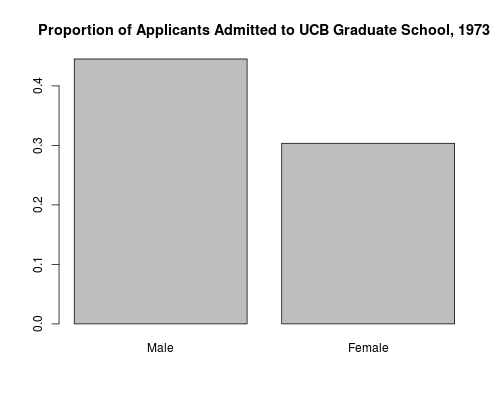
\includegraphics[width = .45\linewidth]{../plots/UCBadmissions.png}
  \end{center}
  
\item [\bf Quantitative variables] are plotted with dot plots, histograms,
  density plots, and boxplots.

  \begin{list}{}{}
  \item [\bf dot plots] represent each point with a dot above the number
    line. This works well with small sample sizes.  If the data are
    too close together to distinguish, we might stack them up to
    remove any overlap. \vspace{-1cm}
%% plot(x=email50$num_char, y = rep(1,50), xlab = "1000 Characters",
%% ylab = "", bty= "n",yaxt="n", cex = 2, pch = 16, col =
%% rgb(0,0,1,alpha = .3))
%% dev.copy(png,"plots/dotplotDemo1.png",height = 200, width = 500);dev.off()

  \begin{center}
  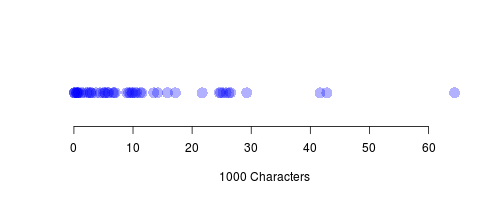
\includegraphics[width = .8\linewidth]{../plots/dotplotDemo1.png}
  \end{center}

  \item [\bf histograms] divide the axis into ``bins'' and count the
    numbers of points falling into each bin.  The height of each bin might
    show the count (frequency) of values in the bin or the proportion
    (relative frequency) for the bin.  These plots work with moderate
    to large sized data sets.  Choosing the best number of bins can be
    hard. \vspace{-.4cm}
%% hist(email50$num_char, xlab = "1000 Characters", main = "")
%% dev.copy(png,"histogramDemo1.png",height = 300, width = 500);dev.off()
  \begin{center}
  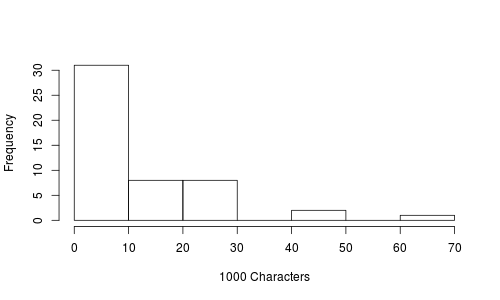
\includegraphics[width = .6\linewidth]{../plots/histogramDemo1.png}
  \end{center}


  \item [\bf density plots] are basically like smoothed off
        relative frequency histograms. \vspace{-.4cm}

%% plot(density(email50$num_char), xlab = "1000 Characters", main = "")
%% dev.copy(png,"densityDemo1.png",height = 300, width = 500);dev.off()
  \begin{center}
  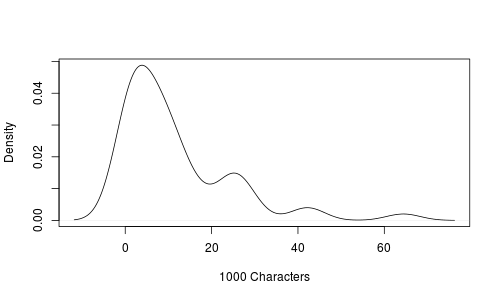
\includegraphics[width = .6\linewidth]{../plots/densityDemo1.png}
  \end{center}

   \item [\bf box-and-whisker plots] show the quartiles of the
     distribution, making a box from $Q_1$ to $Q_3$ (median is also $Q_2$), and
     then showing whiskers which extend to the minimum and maximum
     value. If those extremes are too far out, the whisker usually
     stops at the last point within 1.5 $\times$ IQR's of either
     $Q_1$ or $Q_3$ and flags points beyond 1.5 $\times$ IQR as
     ``outliers'', or unusual points.  
     Half of the data will be included in the box, and half will be
     outside the box. \vspace{-1cm}
%% boxplot(email50$num_char, horizontal = TRUE, xlab = "1000 Characters", main = "")
%% dev.copy(png,"boxplotDemo1.png",height = 200, width = 500);dev.off()
  \begin{center}
  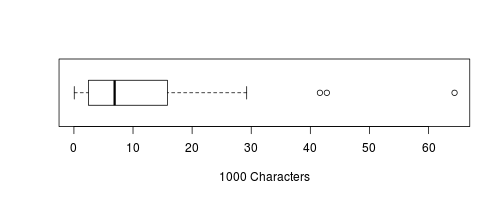
\includegraphics[width = .8\linewidth]{../plots/boxplotDemo1.png} \vspace{-.5cm}
  \end{center}

\end{list}
\end{list}

%%  barplot(prop.table(apply(UCBAdmissions,1:2,sum),2)[1,])
%% title("Proportion of Applicants Admitted to UCB Graduate School, 1973")
%% dev.copy(png,"classes/stat216/TR-F2015/coursePa/plots/UCBadmissions.png",height = 400, width = 500);dev.off()


One more idea is important in describing a sample of quantitative
values is the {\bf skew} of a distribution of values.  \\
  A distribution is skewed if the histogram tapers off to one
  side. For example, the num\_char variable above shows strong right
  skew because the histogram and density plots taper down to the
  right, and the boxplot has a long ``right tail'' (longer whisker to
  right and outliers to right).
\\
 If those same plots look roughly the same on each side, we say the
 data  are ``symmetrically distributed''.


 \begin{center}
   {\large\bf Important Points}
 \end{center}

 \begin{itemize}
    \item From the Syllabus (p 1-5) 
       What portion of your grade comes from D2Quizzes?\\
       from D2Boxes?\\
       from Attendance, Preparation, Participation?
    \item  What is your goal for a grade in this class?\\ \\
       Will you be able to spend 9 hours per week (outside of
       class) to achieve that goal?\\
     \item Who in your group will bring a laptop to the next class?\\

       From pages 10--13:
     \item What are the two main types of data mentioned in this
       reading?\\ \\
     \item What plots are used to display each type of data? \\ \\ \\
     \item How do we summarize each type of data?\\ \\ 

 \end{itemize}  %% buff  p 11 -- 16
  \newpage

\fancyhead[LE,RO]{
   {\it Notes }\\
   {\it Unit \unitNum\   \ Page \thepage }
}
%Intentionally left blank
\phantom{No text here}
\newpage


\fancyhead[LE,RO]{
   {\it \theTopic }\\
   {\it Unit \unitNum\  Activity \dayNum \ Page \thepage }
}
 \def\theTopic{Descriptive Stats }
\def\dayNum{2}

\section{ Got Data?}

Statistics is all about making sense of data, so we first need to pay
some attention to the main types of data we will be using.

\begin{enumerate}
  \item Which  variable is of a  different type?
    \begin{alist}
      \item  The cell phone carrier you use.
      \item  The monthly fee charged by your cell phone provider.
      \item  Whether your cell phone has buttons or touch screen.
      \item  The manufacturer of your cell phone.
    \end{alist}
     Circle the odd ball and explain why its different.
\begin{students}
    \vspace{1cm}    
\end{students}

\begin{key}
  {\it B.  It's numeric, not categorical.}       
\end{key}

\item Got it?  -- Let's just check again for the different data type.
  \begin{alist} \setcounter{alistctr}{4}
    \item Amount you spend on textbooks this term.
    \item Number of credits you're signed up for.
    \item How much student loan you'll take out this term.
    \item The area code of your phone number.
  \end{alist} Again circle one and explain.
\begin{students}
    \vspace{1cm}
\end{students}

\begin{key}
  {\it D.  Area code is categorical. Finding an average for the class
    makes sense for the others, but average area code is meaningless.}       
\end{key}
\end{enumerate}

\label{summry}One thing we need to be comfortable with is
  summarizing data.  As you read in the reading for today, we first
  have to identify the type of variable, then decide how to summarize it.
You've read about two main types of data:
\begin{list}{}{}
\item [\bf Quantitative] takes numeric values which we can average.
\item [\bf Categorical] falls into one of two or more categories.  The
  categories can have numeric labels (like zip codes), but it makes no
  sense to average them. (some call this ``Qualitative'', but we don't
  like to use two words starting with Q) 
\end{list}

\begin{enumerate} 
\setcounter{enumi}{3}
\item  For which variables on the previous page, A through H, would the
  {\bf mean} be informative?
\begin{students}
    \vspace{\fill}    
\end{students}

\begin{key}
  {\it B, E, F, G }
\end{key}
\end{enumerate}

   We also need to summarize categorical data, so we use proportions:
   the number in a certain category divided by the total number.

\begin{enumerate} 
\setcounter{enumi}{4}
\item  For which variables on the previous page, A through H would the
  {\bf proportions} be informative?
\begin{students}
    \vspace*{\fill}    
\end{students}

\begin{key}
  {\it A, C, D, H }
\end{key}
     
\end{enumerate}
  %\newpage
\subsection {Comparing Distributions} %\vspace{-.2in}


 Now we'll focus on quantitative data.    \vspace{-.3in}
 \begin{enumerate}
\setcounter{enumi}{5}
 \item \label{center}
   Suppose you are choosing which professors' class to enroll
     in.  You have three choices, and have data on the grade
     distribution for each shown as histograms.  
     Which class seems to have the best grade distribution? Explain. \\
  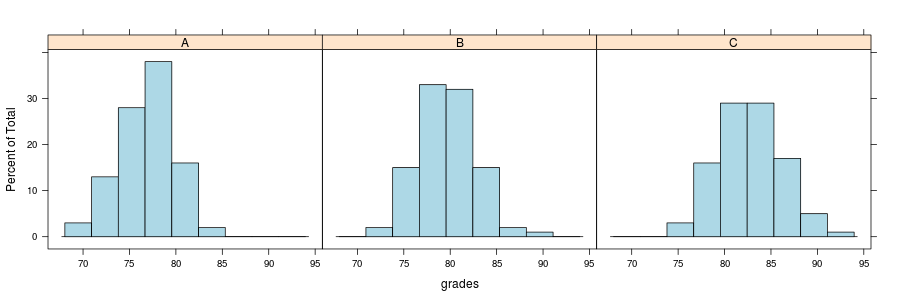
\includegraphics[width = .7\linewidth]{../plots/3classGradeCompareMn.png}
\begin{students}
    \vspace{2cm}    
\end{students}

\begin{key}
  {\it Class C has the largest mean and median, so most will vote for it. }
\end{key}

\item  \label{skew} Here are density plots of  another set of three
  distributions of exams scores. Which do you prefer?  Explain why. 

   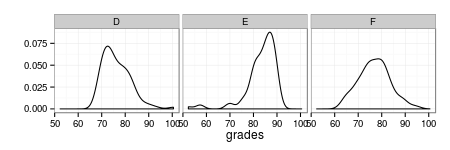
\includegraphics[width=.7\linewidth]{../plots/3classGradeCompareSkw.png}
\begin{students}
    \vspace{2cm}   
\end{students}

\begin{key}
  {\it Class H has more A's than C's, so it's the wise choice.  It
    seems evenly split to high and low grades, while G seems to have
    lots of low grades.}
\end{key}

    
   \item  \label{spread}And here's a third set as a dot plot. Each point is one
     student's exam score -- stacked up when several people have the
     same score.   Which class do you prefer?  Explain the
     differences.  
     
    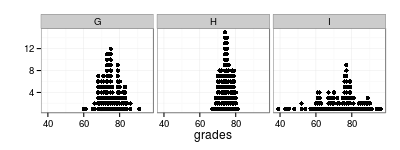
\includegraphics[width=.7\linewidth]{../plots/3classGradeCompareSD.png}
\begin{students}
    \vspace{2cm}
\end{students}

\begin{key}
  {\it The big difference here is in spread.  If you're an ``average''
  student, then you would choose E because almost everyone gets a C and
  there's little chance of flunking.  If you are a good student, then
  F is more attractive since more people get A's in this class.}
\end{key}


  \item  When comparing distributions there are several things to consider:
    \begin{itemize}
    \item  Comparing location or center (measured by mean or median)
      tells us which class did best ``on average''. 
    \item  Comparing spread (interquartile range or standard
      deviation) tells us which class is generally closest to its mean.
    \item  Comparing skew (could be left or right) to symmetric tells
      us which tail stretches out more.
      (Let's hope that there are more high grades than low ones.) 
    \end{itemize}
    In the three problems above, which comparison were you making?
    For each set of comparisons, fill in center, spread, or skew. \\
    (\ref{center} )
\begin{students}
\underline{\hspace*{3cm}}\hfill 
\end{students}
\begin{key}
  \underline{\hspace*{1cm}}  {\it  center} \underline{\hspace*{1cm}}\hfill 
\end{key} 
    (\ref{skew}) 
\begin{students}
   \underline{\hspace*{3cm}}\hfill 
\end{students}
\begin{key}
  \underline{\hspace*{1cm}}  {\it  skewness} \underline{\hspace*{1cm}}\hfill 
\end{key}
    (\ref{spread}) 
\begin{students}
  \underline{\hspace*{3cm}}\hfill 
\end{students}
\begin{key}
  \underline{\hspace*{1cm}}  {\it spread} \underline{\hspace*{1cm}}\hfill 
\end{key}
  \item   Of the three comparisons above, which was easiest and which
    was hardest? Explain. 
\begin{students}
    \newpage
\end{students}

\begin{key}
  {\it  Center is generally the easiest.  One could argue that spread
    is hard because you have to read the scales carefully, plus it
    depends on your amount of ambition for a good grade.  Skew is also
  hard because it require a close comparison of each tail. In this
  case, lots of A's are clearly preferred to an even spread or to more
D's.}
\end{key}



\item 
  You  have read about mean, median, standard deviation, IQR,
  boxplot and histograms.  Apply what you learned
  to these data on   2009 professor's salaries at a college in the US.

   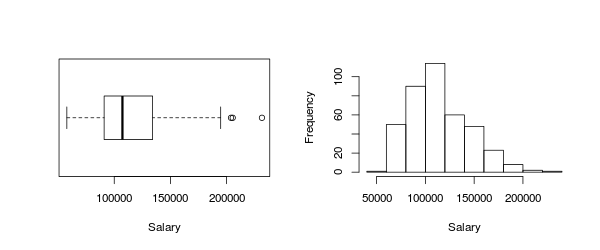
\includegraphics[width=.8\linewidth]{../plots/salaryBoxHist.png}
  \begin{enumerate}
    \item  Is salary skewed (if so which way?) or does it have a
      symmetric distribution? 
\begin{students}
    \vspace{1cm}    
\end{students}

\begin{key}
  {\it  right skewed}
\end{key}

    \item Are any points flagged as outliers?  If so, describe them. 
\begin{students}
    \vspace{1cm}    
\end{students}

\begin{key}
  {\it Three points with salary over \$200,000 are flagged as outliers.}
\end{key}
     \item  Give approximate values for the median and the first and
       third quartiles.  Also compute the IQR.
\begin{students}
    \vspace{1cm}    
\end{students}

\begin{key}
  {\it  Q1: \$90k, Median: \$110k, Q3: \$135K, IQR: \$25k}
\end{key}
    \item For these data, which is a better summary: mean and standard
      deviation?  or median and IQR? Why?
\begin{students}
    \vspace{1cm}    
\end{students}

\begin{key}
  {\it median and IQR -- due to skewness.}
\end{key}
    \end{enumerate}


  \item In Christian Rudder's book {\it Dataclysm} (2014) he shows
    plots of how men rate the attractiveness of women (data from the
    online dating site OKcupid) on a scale of 1 to 5 -- the solid line
    in this plot.  Y axis is the percentage of women who get this
    ranking. The line connects what would be the centers at the top of
    each bar of a histogram, (sometimes called a ``hollow
    Histograms'').  The dashed line was added by forcing in a
    perfectly symmetric distribution. Describe the skew of the solid
    line using the dashed line as a reference.


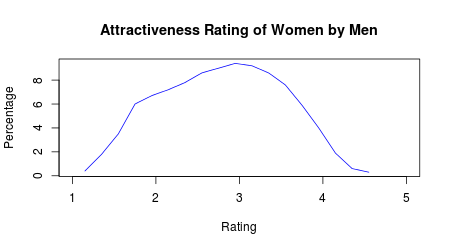
\includegraphics[width=.4\linewidth]{../plots/menRateWomen.png}

\begin{students}
   \   \vspace{2cm}    
\end{students}

\begin{key}
  {\it The solid line is slightly skewed to the right. If womens'
    looks are symmetrically distributed, then men are being a bit hard
  on them, pushing their scores a bit lower.}
\end{key}


\item So men have some ``biases'' about female attractiveness.  What
  if we go the other way and have women rate men?  Are the men using
  OKcupid really ugly?  Describe what's going on here.

 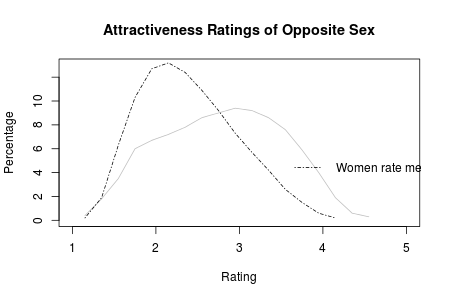
\includegraphics[width=.5\linewidth]{../plots/RateMenAndWomen.png}
\begin{students}
\vfill
\end{students}

\begin{key}
  {\it  Women have stricter standards in what they see as attractive?
     Or are women posting pictures that are showing themselves to
     better advantage than the pictures men choose?}
\end{key}
\end{enumerate}
  



\begin{center}
  {\bf Take Home Message:}
\end{center}
\begin{itemize}
\item To learn about the world, we collect data. Two main types:
  \begin{itemize}
  \item Categorical -- summarize with proportions
  \item Quantitative -- describe center (mean or median) spread (SD
    or IQR) and shape of distribution (symmetric, left-skewed,
    right-skewed). 
  \end{itemize}
\item Plots:
  \begin{itemize}
  \item Categorical -- use bar charts. Pie charts waste ink and are
    harder to read.
  \item Quantitative -- Dot plots, histograms, boxplots.\\
    We describe center (mean or median), spread, and shape based on
    these plots.
  \end{itemize}
\end{itemize} \vfill



{\bf Assignments}
\begin{itemize}
%\item  D2Quiz 1 on D2L by 11 pm Jan 18.
\item %{\bf D2Box 1} - Due 11 pm Jan 21.  
   A template for a ``Box'' assignment is posted on D2L.
  Your completed assignment must be exported as a pdf file and uploaded
  to the D2L dropbox folder  for D2Box \# 1.
\item Read Reading 2 for the next class.
\item View Video \# 2 listed in the videos link. 
\end{itemize}

 %% Descriptives - pgs 17 - 26
 \newpage


\fancyhead[LE,RO]{
   {\it Notes }\\
   {\it Unit \unitNum\   \ Page \thepage }
}
%Intentionally left blank
\phantom{No text here}
\newpage


\fancyhead[LE,RO]{
   {\it \theTopic }\\
   {\it Unit \unitNum\   \ Page \thepage }
}
  \def\theTopic{Reading 2}


 \section{ Population and Sample}


The science of statistics involves using a {\bf sample} to learn about
a {\bf population}.

{\bf Population}: all the units (people, stores, animals, ...) of
interest.

{\bf Sample}:  a subset of the population which gets measured or
observed in our study.

{\bf Cases}:  subjects or units on which information is collected.  

{\bf Variable}:  A quantity of interest which is measured or observed
on units.

{\bf Statistical  Inference}: making a statement about a
{\bf population parameter} based on a {\bf  sample statistic}.

{\bf Parameter}:  a number which describes a characteristic of the
population. These values are never completely known except for small
populations which can be enumerated. We will use:\\
  $\mu$ (pronounced mew) to represent the population mean.\\
  $\sigma$ (pronounced sigma) to represent the population's standard deviation
  (spread).\\
  $p$ (just plain pea) to represent a population proportion.\\
  $\rho$ (the Greek letter ``rho'' which sounds just like row) for
  correlation between two 
  quantitative variables in a population.\\
  $\beta_1$ (read it as beta-one) slope of a true
  linear relationship between  two 
  quantitative variables in a population.

{\bf Statistic}:  a number which describes a characteristic of the
sample and can be computed from the sample. We will use:\\
  $\xb$ (read it as ex--bar) to represent the sample mean (or average value).\\
  $s$  to represent the sample's standard deviation
  (spread).\\
  $\phat$ (read it as pea--hat) to represent a sample proportion.  (We
  often use a hat to  represent a statistic.)\\
  $r$  for correlation between two  quantitative variables in a sample.\\
  $\widehat{\beta}_1$ (beta--hat one) slope of the ``best fitting''
  line  between  two  quantitative variables in a sample.

In this Unit 1, we will focus on parameter $p$ and will use sample
statistic $\phat$ to estimate it.

\begin{center}
  {\bf Representative Samples}
\end{center}

Because we want the sample to provide information about the
population, it's very important that the sample be {\bf
  representative} of the population. \\
In other words: we want the statistic we get from our sample to be
{\bf unbiased}.  Bias creeps in in several ways:
\begin{itemize}
  \item Asking a leading question can bias results.  
  \item Missing a part of a population can bias results.  For example,
    it's very hard to sample the part of the US residents who have
    no home and no phone.
  \item When a web page or a newspaper asks for peoples' opinions, it
    is typically the people with strong opinions who take the time
    to respond. 
\end{itemize}

\begin{center}
  {\bf Sampling problems}:\vspace{-.5cm}
\end{center}
\begin{list}{}{}
\item [\bf Convenience Sample]  is made up of units which are easy to
  measure. For example, to assess people's opinions on federal college
  loan programs, we interview students on a university campus.  Or to
  assess the presence of noxious weeds in the state, we select only plots
  of ground which are within 100m of a secondary highway. 
\item [\bf Non-response bias:] If people refuse to answer questions
  for a phone survey, or do not return a mailed survey, we have a
  ``non-response.'' Non-responses cause bias in the results if those
  who fail to respond differ (in their response) from those who do
  respond. 
\end{list}

\begin{center}
  {\bf Ideal Samples}
\end{center}
 Ideally we will have a list of all units in the population and can
 select units {\bf at random} to be in our sample. 
Random selection assures us that the sample will generally be
representative of the population.\\ \\
 A {\bf simple random sample} is selected so that every sample of size
 $n$ has the same chance of being selected.  You can think of this as
 pulling names out of a hat (although it's better to use the computer
 to select samples since names in the hat might not be well mixed). 

  Simple random sampling is not the only way to get a random
  sample, and more complex schemes are possible.  If you run into a
  situation in which the population is divided into strata (for
  example university students live either on campus, in Greek houses,
  or non-Greek off campus housing, and you want to sample from each)
  you can use a {\bf stratified sample} which combines simple random
  samples from each level into one big sample.  We will only use simple random
  sampling (SRS) in this course, and suggest that you consult a
  statistician or take more statistics classes if you need more
  complexity. 

 Non-response bias can be addressed with more work.  We would have to
 do a second (or further) attempt to contact the non-responders, then 
 check to see if they differ (in some important way) from those who
 responded the first time.  Again, this is a situation in which you
 would need further statistical expertise.

 Bias can also result from the wording of a poll, so writing questions
 is a science in its own right.  People tend to try
 to please an interviewer, so they might, for example, soften their
 attitudes toward breathing second-hand smoke if they know the interviewer
 smokes. 
\newpage

 \begin{center}
   {\large\bf Important Points}
 \end{center}
 \begin{itemize}
 \item Know that we gather data from the {\bf sample} to learn about
   the {\bf population}.
   \begin{itemize}
   \item A number describing a population is called a  
\begin{students}
       \\ \\
\end{students}
\begin{key}
  {\bf parameter.}
\end{key}
   \item A number describing a sample is called a  
\begin{students}
       \\ \\
\end{students}
\begin{key}
  {\bf statistic.}
\end{key}
   \end{itemize}
 \item Why is a representative sample important?  
\begin{students}
       \\ \\
\end{students}
\begin{key}
  {\bf Because we want to learn about the entire population using our sample.}
\end{key}
 \item How can we be sure we are getting a representative sample? 
\begin{students}
       \\ \\
\end{students}
\begin{key}
  {\bf Use random selection.}
\end{key}
 \end{itemize}
   
                               %%  buff: 23 - 26
  \newpage

\fancyhead[LE,RO]{
   {\it Notes }\\
   {\it Unit \unitNum\   \ Page \thepage }
}
%Intentionally left blank
\phantom{No text here}
\newpage


\fancyhead[LE,RO]{
   {\it \theTopic }\\
   {\it Unit \unitNum\  Activity \dayNum \ Page \thepage }
}
 \def\theTopic{Sampling }
\def\dayNum{3}

\section{ Sampling}

If we can measure every unit in a {\bf population}, we then have a
{\bf census} of the population, and  we can 
compute a population {\bf parameter}, for instance a proportion, mean,
median , or measure of spread. However, often it costs too much
\vspace{-.4cm}
\begin{center}
  {\large\bf  time}\hspace{2cm} or\hspace{2cm} {\bf\large money}
\vspace{-.4cm}
\end{center}
      so we cannot take a census.  Instead we  sample from the
      population and compute a {\bf statistic} based on our {\bf
      sample}. The science of statistics is all about using data from
    the sample to make inferences about the population.\\
  This lesson focuses on how to  get a good sample.  We need a way to select
  samples which are representative of the population.
  \\
  The box below contains 241 words which we will treat as our
  population. (This is different from how we usually collect data. In
  practice we never have the entire population. Here we have created a 
  small population to learn how well our methods work.)  
  \begin{enumerate}
  \item  Circle ten words in the passage below which are
     a representative sample of the entire text. (Each person does
     this, not one per group).

   \fbox{ \sf
     \begin{minipage}{1.0\linewidth}
Four college friends were so confident that the weekend before finals,
they decided to go to a city several hours away to party with some
friends. They had a great time. However, after all the partying, they
slept all day Sunday and didn't make it back to school until early
Monday morning. 
 Rather than taking the final then, they decided to find their
 professor after the final and explain to him why they missed it. 
They explained that they had gone to the city for the weekend with the
plan to come back and study but, unfortunately, they had a flat tire
on the way back,  didn't have a spare, and couldn't get help for a
long time. As a result, they missed the final. 
The professor thought it over and then agreed they could make up the
final the following day. 
The four were elated and relieved. 
They studied that night and went in the next day at the time the
professor had told them. 
The professor placed them in separate rooms and handed each of them a test
booklet, and told them to begin. They looked at the first problem,
worth 5 points. It was something simple about exploratory data
analysis. 'Cool,' they thought at the same time, each one in his
separate room. 'This is going to be easy.' 
Each finished the problem and then turned the page. On the second page was written: For 95 points: Which tire?        
     \end{minipage}
}

Note:  Do this quickly.  Our goal will be to use the sample to
estimate average word length in the entire text, but do not try to
study the text too closely. Two minutes should be plenty of time to
select 10 words.  
 
\newpage
\item Did you use any strategy to select words at random?
\begin{students}
  \vspace{1cm}
\end{students}    
\begin{key}
   {\it Answers will vary.  Some will be more representative than others.}
\end{key}


\item Suppose we want to estimate the mean (average) length of all
  words in our population. Is that a parameter or a statistic?
\begin{students}
  \vspace{1cm}
\end{students}    
\begin{key}
   {\it parameter}
\end{key}
\item What is the average word length for your sample?
\begin{students}
  \vspace{1cm}
\end{students}    
\begin{key}
   {\it AWV}
\end{key}

  \begin{center}
    {\LARGE STOP!}\\
Give your sample means to your instructor.
  \end{center}

\item To evaluate a method of estimation, we need to know the true
  parameter and we need to run our method lots of times.  That's why
  we chose a small population which we know has mean word length of
  4.29 letters. (Where does 4.29 appear in the web app?).  You are
  giving your estimate to your instructor so that we can see how well
  your class does as a whole.  In particular we want to know if people
  tend to choose samples which are biased in some way. To see if a
  method is biased, we compare the distribution of the estimates to
  the true value.  We want our estimate to be
  \begin{center}
    {\large on target = unbiased.}\\
  Then the mean of the distribution matches our true parameter.
  \end{center}
  While we're waiting to collect everyone's sample mean we will look
  at another method:
 
    \subsection{ Simple Random Sampling}
 
  \begin{enumerate}
    \item Point your browser to \webAppURLFrst.

 Bookmark this page, as we'll come back here often.  

 Click on \fbox{One Quant.} because we are dealing with one
 quantitative variable -- word length -- and drop down to
 \fbox{Sampling Demo}.
     

   \item   The joke text should appear in the gray box. You can drag
     across this text and delete it if you want to paste other text
     into the box, but leave it there now.\\
     % Copy the word length data from D2L.  Select the entire file
       % with control-A, copy it to the clipboard with control-C (or use
       % the right mouse button to copy) and paste it into the applet's
       % data box (use control-V or the mouse option). 
       Click \fbox{Use This Text}.  You
       should see a plot of all word lengths with summary
       information.  This is our population of 242 words.
     \item  Set \fbox{Sample Size} to \fbox{10} and click \fbox{Draw
           one Sample}.   Write out the 10 words and their lengths.  
\begin{students}
  \vspace{2cm}
\end{students}    
\begin{key}
   {\it AWV }
\end{key}      
    \end{enumerate}
     \item  Record the average (mean) word length for the ten
       randomly sampled words. Remember, your sample average is an
       estimate of the average word length in the population.  
\begin{students}
  \vspace{1cm}
\end{students}    
\begin{key}
   {\it AWV}
\end{key}

     \item  Click  \fbox{Draw one Sample} again and record the next mean.
\begin{students}
  \vspace{1cm}
\end{students}    
\begin{key}
   {\it AWV}
\end{key}
       

     \item  Click the ``More Samples:'' choices to
       obtain at least \fbox{3000} more samples. Record the mean and
       standard deviation of all 
       the  sample means. (See upper right of the plot.)       
\begin{students}
  \vspace{1cm}
\end{students}    
\begin{key}
   {\it Should be close to 4.29 for mean, 0.60 for st.dev }
\end{key}
         

\item \label{3000SRSs} If the sampling method is unbiased, the
  estimates of the population average (one from each sample of size
  10) should be centered around the population average word length of
  4.29.
  Does this appear to be the case? \\
  Copy the plot here and describe what you see.
\begin{students}
  \vspace{3cm}
\end{students}    
\begin{key}
   {\it Should see a slightly right-skewed distribution with center
     close to 4.29.  Mine go from 2.6 to 6.8. }
\end{key}

     \item  Click on the leftmost blue dot. The ``Sample Words''
       change to show you the sample with the smallest average. How
       many one-letter words are in this sample?  Copy the sample and
       its mean here:
\begin{students}
  \vspace{1cm}
\end{students}    
\begin{key}
   {\it Only 1 {\sf a, at a with the the up to but the was}   Mean: 2.6}
\end{key}
     \item  Click on the rightmost blue dot. What is your longest
       word?   Copy  its mean here:
\begin{students}
  \vspace{1cm}
\end{students}    
\begin{key}
   {\it {\sf unfortunately} (13) Mean: 6.8}
\end{key}


     \item\label{classPlot} {\bf Class Samples} Now your instructor will
       display the  estimates from each person in the class. 
        Sketch the plot of all of the sample estimates. 
        Label the axes appropriately.       
\begin{students}
  \vspace{4cm}
\end{students}    
\begin{key}
   {\it Hope to see some bias here.  Discuss estimates close to
     4.29. Did they use a strategy?}
\end{key}

      \item  The actual population mean word length based on all 242
        words is 4.29 letters. Where does this value fall in the
        above plot? Were most of the sample estimates around the
        population mean? Explain. 
\begin{students}
  \vspace{1cm}
\end{students}    
\begin{key}
   {\it Expect them to say: No, we got fooled into picking the larger words.}
\end{key}     

     \item\label{medUnbiased} For how many of us did the sample
       estimate exceed the population mean? What proportion of the
       class is this?        
\begin{students}
  \vspace{1cm}
\end{students}    
\begin{key}
   {\it AWV, but more than half, I expect.}
\end{key}

     \item Based on your answer to question \ref{medUnbiased}, are 
       ``by eye'' sample estimates just as likely to be above the population
       average as  to be below the population average?  Explain.      
\begin{students}
  \vspace{1cm}
\end{students}    
\begin{key}
   {\it No, they are biased to generally be larger.}
\end{key}

     \item Compare the applet plot from question \ref{3000SRSs} with
       the plot from \ref{classPlot}.  Which method is closer to being {\bf
         unbiased}? Explain.
\begin{students}
  \vspace{3cm}
\end{students}    
\begin{key}
   {\it  Random sampling should win the day here.  It is unbiased.}
\end{key}
     
     \end{enumerate}
     
       \subsection{ Examining the Sampling Bias and Variation}

       To really examine the long-term patterns of this sampling
       method on the estimate, we use software to take many, many
       samples. {\bf Note}: in analyzing real data, we only get {\bf
         one} sample. This exercise is {\bf NOT} demonstrating how to
       analyze data. It is examining how well our methods work in the
       long run (with many repetitions), and is a special case when
       we know the right answer.

       We have a strong preference for unbiased methods, but even when
       we use an unbiased estimator, the particular sample we get
       could give a low or a high estimate.  The advantage of
       an unbiased method is {\bf not} that we get a great estimator
       every time we use it, but rather, a ``long run'' property when
       we consider using the method over and over.

       Above we saw that Simple Random Sampling gives
       unbiased estimates.  People picking a representative sample are
       often fooled into picking more long than short words.  Visual
       choice gives a biased estimator of the mean.

       Even when an unbiased sampling method, such as simple random
       sampling, is used to select a sample, you don't expect the
       estimate from each individual sample drawn to match the
       population mean exactly. We do expect to see half the estimates
       above and half below the true population parameter.

       If the sampling method is biased, inferences made about the
       population based on a sample estimate will not be valid. Random
       sampling avoids this problem.   Next we'll examine the role of
        sample size.  Larger samples do provide more
        information about our population (but they do not fix a problem
        with bias).

        \begin{center}
         {\large \sf Does changing the sample size impact whether the
           sample estimates are unbiased?} 
       \end{center}
     
     \begin{enumerate}
       \setcounter{enumi}{16}
     \item Back in the web app, change ``Sample Size'' from 10 to \fbox{25}. 
       Draw at least 3000 random samples of 25 words, and write down
       the mean and standard deviation of the sample means.
\begin{students}
  \vspace{1cm}
\end{students}    
\begin{key}
   {\it  AWV. Std Dev should be smaller.}
\end{key}

     \item \label{size25} Sketch the plot of the sample estimates based on the
       3000 samples drawn. Make sure to label the axis appropriately. 
       \begin{students}
  \vspace{3cm}
\end{students}    
\begin{key}
   {\it  AWV}
\end{key}

     \item  Does the sampling method still appear to be unbiased? Explain.
       \begin{students}
  \vspace{1cm}
\end{students}    
\begin{key}
   {\it  Yes, because the distribution is centered at the true mean.}
\end{key}

     \item  Compare and contrast the distribution of sample estimates
       for $n = 10$ and the distribution of sample estimates for $n =
       25$. How are they the same? How are they different?  
       \begin{students}
  \vspace{2cm}
\end{students}    
\begin{key}
   {\it  Same in that both are centered at 4.29.  Different in that
     the st.dev is larger for $n=10$ (it is 0.60) than for $n = 25$
     (0.38). }
\end{key}

     \item Compare the spreads of the plots in \ref{3000SRSs} and
       \ref{size25}.   You should see that in one plot all sample
       means are closer to the population mean than in the other.
       Which is it? Explain.
\begin{students}
  \vspace{1cm}
\end{students}    
\begin{key}
   {\it  Sample size 25.}
\end{key}

\item Using the evidence from your simulations, answer the following
  research questions. Does changing the sample size impact whether the
  sample estimates are unbiased?  Does changing the sample size impact
  the variability of sample estimates?  If you answer yes for either
  question, explain the impact.
       \begin{students}
  \vspace{2cm}
\end{students}    
\begin{key}
   {\it  Yes, as sample size gets bigger, the st.dev goes down.}
\end{key}
 
\begin{students}
  \newpage
\end{students}

%        \subsection  { Population Size}


%        Now we examine another question:
%        \begin{center}
%          {\sf  Does changing the size of the population impact whether
%            the sample estimates are unbiased?} 
%        \end{center}


%      \item  Increase the size of the population. 
%        Click  \fbox{Clone (double) the Text} under the data box {\bf
%        two times}. 
%        How large a population do you now have?  Does the mean change?
%        \begin{students}
%   \vspace{1cm}
% \end{students}    
% \begin{key}
%    {\it  968. mean (and SD) stay the same.}
% \end{key}

%      \item With sample size set to \fbox{25}, draw a few single
%        samples to see if they look similar, then 
%        draw 3000 or more random samples and record the average
%        (mean) of all the average word lengths.
%        \begin{students}
%   \vspace{1cm}
% \end{students}    
% \begin{key}
%    {\it  AWV. I got mean 4.286, SD = 0.382}
% \end{key}

%      \item  Sketch the plot of the sample estimates based on the 1000
%        samples drawn. Label the axis appropriately. 
%        \begin{students}
%   \vspace{3cm}
% \end{students}    
% \begin{key}
%    {\it  Hope to see center and spread have not changed much.}
% \end{key}

    %  \item  Record the mean and standard deviation of the sample averages.
%        \begin{students}
%   \vspace{2cm}
% \end{students}    
% \begin{key}
%    {\it  AWV}
% \end{key}

 %     \item  Does the sampling method still appear to be unbiased?
%        Explain.
%        \begin{students}
%   \vspace{3cm}
% \end{students}    
% \begin{key}
%    {\it  Yes.  It's centered at about 4.29.}
% \end{key}

%      \item Compare and contrast the distribution of sample estimates
%        for $n = 25$ now that you are sampling from a larger population
%        to the distribution of sample estimates for $n = 25$ from
%        before. How are they the same? How are they different?
%        \begin{students}
%   \vspace{3cm}
% \end{students}    
% \begin{key}
%    {\it  Means of the two distributions are essentially the same, std dev
%      also is the same.}
% \end{key}

%      \item Use the evidence collected from the simulation to answer
%        the research question: does changing the size of the population
%        impact whether the sample estimates are unbiased?
%        \begin{students}
%   \vspace{4cm}
% \end{students}    
% \begin{key}
%    {\it  No.  The sample mean for 25 observations has roughly the same
%      mean and st.dev as it did with 241 in the population.}
% \end{key}

     \item When we actually collect data, we only get a single sample.
       In this exercise, we started with a known population and
       generated many samples. How did we use many samples to learn
       about properties of random sampling?
\begin{students}
  \vspace{1.5in}
\end{students}    
\begin{key}
   {\it  We sampled over and over to see how variable our statistics
     will be.  We compared SE's for different sample sizes and
     population sizes. }
\end{key}

  \end{enumerate}

  A rather counter-intuitive, but  crucial fact is that when
  determining whether or not an estimator produced is unbiased, the
  size of the population does not matter. Also, the precision of the
  estimator is unaffected by the size of the population. For this
  reason, pollsters can  sample just 1,000-2,000 randomly selected
  respondents and draw conclusions about a huge population like all US
  voters. 

  \begin{center}
    {\bf Take Home Messages}
  \end{center}
 
  \begin{itemize}
  \item Even with large samples, we could be unlucky and get a
    statistic that is far from our parameter.
  \item A biased method is not improved by increasing the sample size.
    The Literary Digest poll:\\
    \url{http://en.wikipedia.org/wiki/The_Literary_Digest#Presidential_poll
    } of 2.4 million
    readers was way off in projecting the presidential winner because
    their sample was biased.
    If we take a random sample, then we can make inference back to the
    population. Otherwise, only back to the sample.

  \item Increasing sample size reduces variation.  Population size
    doesn't matter very  much as long as the population is large
    relative to the sample size (at least 10 times as large).
  \item Add your summary of the lesson.  What questions do you have?
  \end{itemize}\vspace{\fill}


 {\bf Assignment}
 \begin{itemize}
 %\item D2Box 1 due Jan 21  11 pm.
 \item %{\bf D2Quiz 2} due Jan 25th 11 pm. 
   For D2L QUizzes, remember: you can save and come
   back, but once you hit ``submit'' you cannot change any answers.
 \item Reading 3 on Helper--Hinderer research. 
 \item View Helper, Hinderer, and ``Ethics for Babies'' posted as 3a --
   3c  and video \# 4 in the videos link before  the next class.
 \end{itemize}

  %% sampling exercise  pgs 27 - 32
                               %% 
 \newpage

% \ \ \ \thispagestyle{empty}
% \newpage

\fancyhead[LE,RO]{
   {\it Notes }\\
   {\it Unit \unitNum\   \ Page \thepage }
}
%Intentionally left blank
\phantom{No text here}
\newpage


\fancyhead[LE,RO]{
   {\it \theTopic }\\
   {\it Unit \unitNum\   \ Page \thepage }
}
  \def\theTopic{Reading 3}


\section{ Ethical Instincts of Babies?}


Researchers at Yale University were interested in how soon in human
development children become aware of (and start to favor) activities
that help rather than hinder others.\\
Title: ``Social evaluation by preverbal infants''
\\
Authors: J. Kiley Hamlin, Karen Wynn \& Paul Bloom
\\
Journal: {\it Nature} 450, 557-559 (22 November 2007) 
\\
Abstract \vspace{-.5cm}
\begin{quotation}
  The capacity to evaluate other people is essential for navigating the
social world. Humans must be able to assess the actions and intentions
of the people around them, and make accurate decisions about who is
friend and who is foe, who is an appropriate social partner and who is
not. Indeed, all social animals benefit from the capacity to identify
individuals  that may help them, and to distinguish these
individuals from others that may harm them. Human adults evaluate
people rapidly and automatically on the basis of both behavior and
physical features, but the origins and
development of this capacity are not well understood. Here we show
that 6- and 10-month-old infants take into account an individual's
actions towards others in evaluating that individual as appealing or
aversive: infants prefer an individual who helps another to one who
hinders another, prefer a helping individual to a neutral individual,
and prefer a neutral individual to a hindering individual. These
findings constitute evidence that preverbal infants assess individuals
on the basis of their behavior towards others. This capacity may
serve as the foundation for moral thought and action, and its early
developmental emergence supports the view that social evaluation is a
biological adaptation. 



The following were randomized across subjects:
(1) color/shape of helper and hinderer; (2) order of helping and
hindering events; (3) order of choice and looking time
measures; and (4) positions of helper and hinderer. 
\end{quotation}

\begin{center}
        {\large\bf Strength of Evidence}
 \end{center}
      The observed result gets compared to the distribution from the
      simulation to gauge the evidence against $H_0$.  That's
      how the scientific method works.  We formulate a hypothesis
      which can be falsified, then see if the data collected argue
      against the hypothesis. Sometimes our result provides a lot of
      evidence against the null model  -- when the observed result is very
      unlikely -- while other times it has very little evidence against
      the null model -- when the observed result is likely under the null
      model. To explain to others  how likely or unlikely the
      observed result is under the null model, we  report the
      ``strength of evidence'' -- also called  the p-value.

       {\bf Definition:} The p-value is the probability of seeing the observed 
       result or something more  extreme if the null
       hypothesis is true. 
 
       We quantify the strength of evidence by answering the question:
       ``If $H_0$ is true, what proportion of the simulated results
       are as unusual as (or even more unusual than) the observed
       result?''  For example, consider the results from ``Martian
       Alphabet'' in Figure 1. A group of 12 humans had 9 correct
       matches and 3 incorrect. The simulation assumed $H_0: p = 0.5$,
       and counted the number of heads in 12 flips of a fair
       coin. (Head $\leftrightarrow$ Correct).  The whole process was
       simulated 1000 times and the number of outcomes at 9 or above
       on the plot are those as extreme or more extreme as the group's
       score. The chance is 74/1000 = 0.074 of getting a result this
       extreme when $H_0$ is true.  The p-value of 0.074 is the
       strength of evidence against $H_0$ for 9 correct matches. It is
       the probability of obtaining results as extreme or more extreme
       when $H_0$ true. 

 \begin{figure}[h]
   \centering
  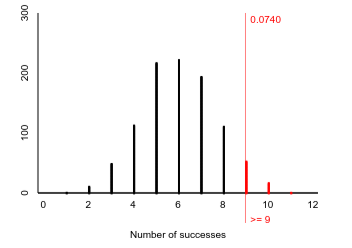
\includegraphics[width=.5\linewidth]{../plots/StrOfEvidence-12Guesses.png}

   \caption{ Simulation results obtained from the null model. The
      outcomes 9 and higher (74 out of 1000 trials) were as or more extreme
      as one group's number correct (of 12) and indicate the strength of
      evidence $=$ 0.074. }
   \label{fig:SOE-12}
 \end{figure}
  For this group of 12, we would say that there is some evidence that
  they can read Martian, but while an  event which can happen  7\% of
  the time is   fairly rare, it may not be totally convincing.  
  A p-value  of 0.07 is not really tiny, but is  a ``cautionary'' yellow
  light. 

 \begin{center}
   {\large\bf Important Points}
 \end{center}
 \begin{itemize}
 \item From the abstract, what was the research question?\vspace{1cm}
 \item What response was recorded? What type of variable is the
   response? \vspace{1cm}
 \item How was randomness utilized?\vspace{1cm}
 \item Would an outcome of 10 or of 8 provide stronger evidence
   against the null than our observed outcome of 9?\vfill
 \item Do smaller or larger p-values provide strong evidence against
   the null hypothesis? 
 \end{itemize}



  %% p 33- 36 buff
  \newpage

\fancyhead[LE,RO]{
   {\it Notes }\\
   {\it Unit \unitNum\   \ Page \thepage }
}
%Intentionally left blank
\phantom{No text here}
\newpage


\fancyhead[LE,RO]{
   {\it \theTopic }\\
   {\it Unit \unitNum\  Activity \dayNum \ Page \thepage }
}
 
\def\theTopic{Helper--Hinderer }
\def\dayNum{4}



 \section{ Helper -- Hinderer}


Do young children know the difference between helpful and unhelpful
behavior?  You read about a study in   {\it Nature}\footnote{ Hamlin, J. K.,
  Wynn, K., \& Bloom, P. (2007). Social evaluation by preverbal
  infants. {\it Nature}, 450, 557-559. } which
reported results from a simple study of infants which was intended to
check young kids' feelings about helpful and non-helpful behavior.  
  The research question is:
\begin{center}
  {\sf Are infants able to notice and react to helpful or hindering
    behavior observed in others?} 
\end{center}

{\bf Data}:  Of the 16 infants age 6 to 10 months, 14 chose the ``helper'' toy
and 2 chose the ``hinderer''.

{\bf Discuss with your group and fill in:	}\vspace{-.3cm}
\begin{enumerate}
  \item  What proportion of the infants chose the helper toy? Include
    the correct notation. ($p$ for a population proportion, or
    $\phat$ for the sample proportion.)
\begin{students}
     \vspace{1cm}
\end{students}

\begin{key}
     {\it  $\phat = 14/16 = 0.875$ }
\end{key}
\item  
     Suppose the infants really had no preference for one toy or the other,
     and the puppet show had no effect.  What sort of results
     (numbers) would     you expect to see?
\begin{students}
       \vspace{1cm}
\end{students}

\begin{key}
       {\it  Close to 1/2 picking the helper.}
\end{key}

   \item Think back to our ``Martian Alphabet'' activity on the first day of
     class.  What sort of evidence made us think that humans could
     decipher Martian script?  Note:  it depended not just on how many
     people in the class got it right, but also on 
     the ``background'' distribution from the coin flips or the spinner.
\begin{students}
  \vspace{2cm}
\end{students}

\begin{key}
       {\it   We saw that relative to the spinner, the the class got
         an unusually high number correct.}
\end{key}
 
   \item How could you use coin flips to model a child's choice of
     toy? For 16 kids?
\begin{students}
  \vspace{2cm}
\end{students}

\begin{key}
       {\it  For one kid, let Heads = ``Helper'', tails =
         ``Hinderer''.  Count the proportion of heads in 16 flips of a
         fair coin.} 
\end{key}
   \item In using the coin, what assumption are you making about the
     kids' preferences? 
\begin{students}
  \vspace*{2cm}
\end{students}

\begin{key}
       {\it   That they are just picking one toy at random with no
         real preference for the helper or hinderer.}
\end{key}

   \item In statistical language the idea of ``no preference'' is
     called the {\bf null hypothesis}  and it is written in terms of
     the population proportion, $p=$ the true proportion of infants
     who chose the helper toy, as
      $$ H_0:\ p = 0.5.$$
     We also have an {\bf alternative hypothesis}, labeled $H_a$,
     which tells us the direction the researchers would like to
     conclude is true.  For this situation, they think there might be
     a preference toward the helper, so they would like to conclude
     that $H_0$ is wrong, and that really 
       $$H_a: \ p > 0.5 \mbox{ is true.}$$

     Under $H_0$,  is it possible that 14 out of 16
      infants could have chosen the helper toy just by chance? 
\begin{students}
  \vspace{1cm}
\end{students}

\begin{key}
{\it Yes, it is possible to get 14 or more heads. Anything is
  possible in a random sequence, but it is not very likely. }
\end{key}

\item If infants had no real preference, would the observed result (14
  of 16 choosing the helper) be very surprising or somewhat
  surprising, or not so surprising? How strong do you believe the
  evidence is against the null hypothesis?
\begin{students}
  \vspace{2cm}
\end{students}

\begin{key}
{\it Pretty surprising, strong evidence against the null.}
\end{key}

%% Use a spinner here?

  \item         {\bf Carry Out the Simulation}\\
     To see that happen, use the
     \webAppURLFrst\  web app. Under
     the \fbox{One Categ} menu select \fbox{Spinner}.  Set the  
        Number of categories to \fbox{2}, Labels to \fbox{help, hinder},
        Percentages to \fbox{50,50}, Stop after \fbox{Fixed number of
          spins}, Last spin: \fbox{16}, and click \fbox{Run} to
        see a simulation of 16 kids choosing helper or hinderer when
        the two are equally likely. Record the number of ``helpers'',
        click \fbox{Run} again, and write down that number as well.
\begin{students}
  \vspace{1.5cm}
\end{students}

\begin{key}
{\it 12 in my first, 8 in my second }
\end{key}

    \item  Set  \fbox{1000} or more trials,  \fbox{Run}, and   
              sketch your plot of 1000 trial results. 
\begin{students}
  \vspace{4cm}
\end{students}

\begin{key}
    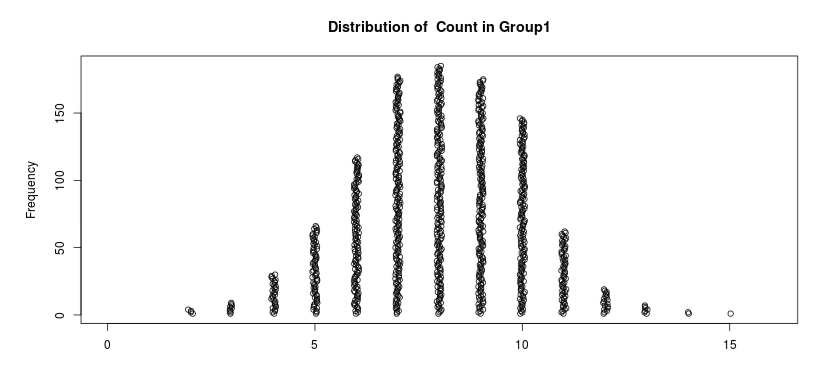
\includegraphics[width=.8\linewidth]{../plots/Helper16.png}
\end{key}
\item To see how unusual it is to get 14 or more ``helpers'' add the
  counts (for 14, 15, 16) in the table below the plot. Note: the
  direction we go from the observed 14 is toward higher values because
  the alternative, $H_a$ was defined as $p > 0.5$ with the inequality
  pointing to the right.  
   How many of yours are this extreme? Circle
  these dots on your plot above. Check with the other groups
  nearby. Do we all agree?
\begin{students}
  \vspace{1.5cm}
\end{students}

\begin{key}
{\it  AWV, typically zero to 5.
}
\end{key}
\item  Do you think that babies are just randomly choosing one of
      the toys? Explain.
\begin{students}
  \vspace{1.5cm}
\end{students}

\begin{key}
  {\it No, because it is unlikely that the observed result will pop up
    if  kids are really picking at random. }
\end{key}

  \end{enumerate}
  You read about p-value or ``Strength of evidence'' in the reading
  for today.   To help interpret strength of evidence, we offer this picture:
 \begin{figure}[h]
   \centering
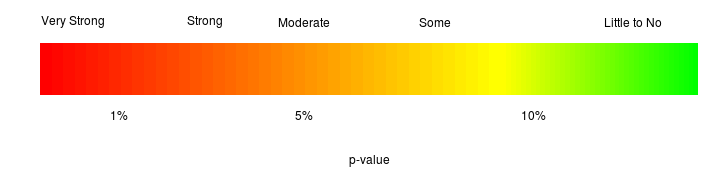
\includegraphics[width=\linewidth]{../plots/pvalueStrengths.png}
   \caption{Numeric p--value and strength of evidence}
   \label{fig:SOE-pvalue}
 \end{figure}

  The important point is that {\bf smaller} p--values (in red) provide {\bf
    stronger} evidence against $H_0$ and then $H_0$ gets a ``red
  light''. Red indicates that we don't believe it.  We will soon talk
  about actually rejecting $H_0$ when the evidence against it is
  strong.  Notation to watch:  strong evidence is always against the
  null. We never have strong evidence in favor of the null.  



\begin{enumerate}
  \setcounter{enumi}{11}

    \item  Use your plot from above to quantify the strength of
      evidence for the observed result 
      of 14 out of 16 infants choosing the helper toy. Give the
      numeric p--value  and a verbal description of the evidence it provides.
\begin{students}
  \vspace{1.5cm}
\end{students}

\begin{key}
{\it  1/1000 on my simulation which is ``Very Strong'' evidence
  against $H_0$.}
\end{key}

\item Explain in your own words why {\bf smaller} p-values provide
  {\bf stronger}   evidence against $H_0$.
\begin{students}
  \vspace{2cm}
\end{students}

\begin{key}
{\it AWV}
\end{key}

\item  What does this suggest about infants making their
      selections based only on random chance?
\begin{students}
  \vspace{2cm}
\end{students}

\begin{key}
{\it It suggests they do not make their choices based on random
 chance and do make decisions based on social interactions. }
\end{key}
\item Summarize how the p-value is computed.
\begin{students}
  \vspace{2cm}
\end{students}

\begin{key}
{\it By comparing the observed result to a distribution we get when
  $H_0$ is true. Take the points as or more extreme and divide by the
  number of points.}
\end{key}

\item  Put the following steps into their proper order:
 \begin{enumerate}
      \item  report strength of evidence 
\begin{key}
          {\it 5}
\end{key}
      \item  gather data 
\begin{key}
        {\it  2}
\end{key}

      \item  formulate a hypothesis 
\begin{key}
{\it 1   }
\end{key}


      \item  simulate a distribution 
\begin{key}
        {\it  3}
\end{key}
      \item  compare observed results to the distribution 
\begin{key}
        {\it  4}
\end{key}

  \end{enumerate}

\item Suppose another researcher had done similar study before this
  one and thinks that the proportion of all infants favoring helper is
  really 0.75.  Change the spinner app to reflect this new hypothesis,
   compute a new p-value, and report the strength of evidence
  against $p = 0.75$.  

\end{enumerate}

{\bf Take Home Messages}
\begin{itemize}
  \item Setting up null and alternative hypotheses is very
    important.\\
    They should be set in the planning stages of the study, not after
    looking at the data. 
    The equals sign always goes into $H_0$, but the value we set $ = p$ is not
    always .5.  The direction of the inequality in $H_a$ must match
    the researcher's ideas -- what they would like to show. It can be
    $<$, $>$, or $\neq$.  The latter means they are looking for a
    difference in either direction.
  \item It's important to know the definition of the p--value. We
    assume $H_0$ is true to compute it.  We  use a simulation based
    on the  value for $p$  in $H_0$ to calculate the p--value.    
  \item The idea of p--value is very important in statistics. It will
    follow us all the way through the course. Stronger evidence means
    {\bf smaller} p--value.  Large p--values mean the data are not
    unusual under $H_0$.
  \item In any hypothesis test, we report p--values to the reader.  
\end{itemize}\vfill

{\bf Assignment}
\begin{itemize}
%\item   D2Quiz 2 on D2L by 11 pm Jan 25.
%\item  {\bf D2Box 2} is due Jan 28.  Turn in as a pdf file to the D2L
%  drop box.
\item The last page of this course pack  is a review table. You should
  tear it out and fill it in as we go. You will be able to bring it
  with you to exams.  You can now fill in the top five boxes  in column 1.
\item Read the next two pages before the next class.
\item Watch video \#  5 on randomization distributions and
  hypothesis testing before class.  Review \# 4 as well.
 \item 
  Make your own summary of the lesson. \\
  Thinking back about the most important ideas of this lesson help
  cement them in your head and help you avoid cramming right before
  the exam.  Writing them here will make studying much easier.   
\end{itemize}


  %% helper-hinderer  pgs 37 - 40 
 \newpage

%
\fancyhead[LE,RO]{
   {\it Notes }\\
   {\it Unit \unitNum\   \ Page \thepage }
}
%Intentionally left blank
\phantom{No text here}
\newpage


\fancyhead[LE,RO]{
   {\it \theTopic }\\
   {\it Unit \unitNum\   \ Page \thepage } 
}
  \def\theTopic{Reading 4}


\section { Extra Sensory Perception}


In the next classroom activity, we will look at an experiment conducted to see
if a person could read another's mind. 

 In the 1930's Dr.~J.B.~Rhine at Duke University designed experiments
to see if some undergraduate students could tell which card (see the
five ``Zener'' cards below) a ``sender'' was looking at. The deck of
cards (5 of each type) was shuffled and a card drawn at random. After
each attempt, the card was returned to the deck and the deck was
reshuffled (we call this sampling with replacement).  Therefore each
of the five card types has an equal chance of occurring at any draw.
\begin{center}
  
\includegraphics[width=.5\linewidth]{../plots/Zener_cards.png}
\end{center}

 Rhine found one exceptional subject in his extrasensory perception
 (ESP) research, Adam Linzmayer, an economics undergraduate at Duke.
 Linzmayer went through the experiments in 1931, and correctly
 identified 36\% of 25 cards as the ``receiver'' in the study. 

We will use Rhine's data, but we want you to know that research into ESP
(also called the ``psi'' effect) has continued.

  Go to this blog and read the Skeptic's report on recent ESP
  research.\\
  \url{https://skeptoid.com/episodes/4348}\vspace{1cm}


  Pay particular attention to how the researchers designed the
  experiment to remove all possible forms of communication between the
  individuals.  \vspace{1cm}


  What is the ``file drawer'' effect?\vspace{1cm}

  What does the author find refreshing and unique about researchers
  studing the ganzfeld effect?\vspace{1cm}



\newpage

In the next activity, we will use a spinner to generate random outcomes. 

To prepare for that, We'd like you to use the circle below (divided
 into 25 equal parts) to  build a ``Wheel of Fortune'' (just like on
 the game show)  with the following chance of each outcome:

\begin{tabular}{l|r}
Outcome & Chance\\ \hline
\$2500  & .04\\
\$1000  & .08\\
\$900  & .12\\
\$800  & .08\\
\$700  & .12\\
\$650  & .08\\
\$600  & .08\\
\$550  & .08\\
\$350  & .08\\
\$100 & .04\\
\$1 million & .02\\
Bankrupt  & .10\\
free play & .04\\
Lose a turn& .04\\
\hline
\end{tabular}
\begin{minipage}{.70\linewidth}
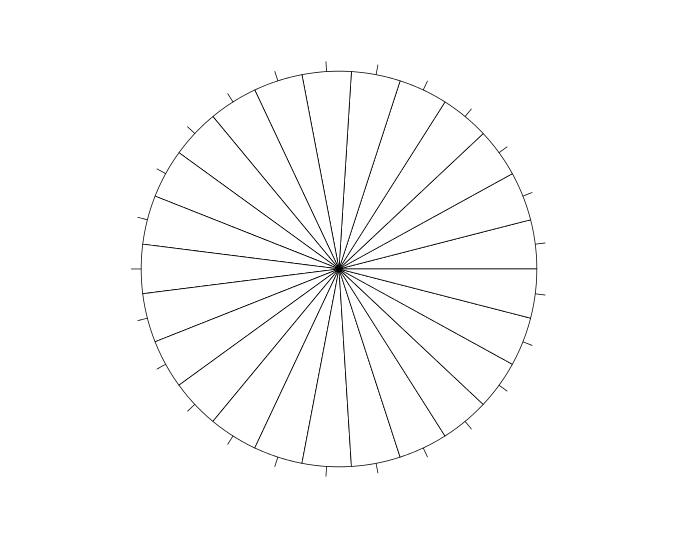
\includegraphics[width = 6in]{../plots/wheelOfFortune.png}
\end{minipage}

In the game show, they mix the outcomes up and give them different
colors. It's fine if you want to do that, but we really want you to
practice getting the right proportions, so putting, for example, all
the \$900 wedges together is fine.


\begin{center}
  {\large\bf Important Points}
\end{center}
\begin{enumerate}
\item How could the ganzfeld experiment go wrong if the scientists
  were not very careful? \vfill

\item What was the chance the subject would -- just by chance --  pick
  the right object (or video) when given the choices?\vfill 

\item On the real ``Wheel of Fortune'' do all outcomes have the same
  chance of getting picked by the pointer when the wheel stops?
\end{enumerate}


 %% p 41- 44 buff
  \newpage


\fancyhead[LE,RO]{
   {\it Notes }\\
   {\it Unit \unitNum\   \ Page \thepage }
}
%Intentionally left blank
\phantom{No text here}
\newpage


\fancyhead[LE,RO]{
   {\it \theTopic }\\ 
   {\it Unit \unitNum\  Activity \dayNum \ Page \thepage }
}
 \def\theTopic{ESP}
\def\dayNum{5}


\section { Can Humans Sense Each Others' Thoughts?}


  We will investigate the data from Adam Linzmayer who correctly
  identified 9 of 25 Zener cards.  Do these data show that
  Linzmayer had extrasensory perception?  More broadly, Rhine wanted
  to know if anyone can catch a signal sent from another's mind using
  no other form of communication.

{\bf Step 1. State the research question. }\\
1. Based on the description of the study, state the research question.
\begin{students}
  \vspace{2cm}
\end{students}

\begin{key}
{\it  Can any person tell what someone else is looking at with no
  other form of communication?.}
\end{key}



{\bf Step 2. Describe the study design and report the data collected.}\\
 Linzmayer was tested 25 times, and correctly identified the card 9
 times in one trial.\vspace{-.3cm}
 \begin{enumerate}
   \setcounter{enumi}{1}
   \item  What was recorded for each guess?
\begin{students}
  \vspace{1cm}
\end{students}

\begin{key}
{\it Right or Wrong}
\end{key}

\item Your answer above gives the outcomes of the variable of interest
  in the study.  Is this variable quantitative or categorical?
\begin{students}
  \vspace{1cm}
\end{students}

\begin{key}
{\it Categorical}
\end{key}
  
   \end{enumerate}
   
{\bf Step 3. Explore the data. }\\
With categorical data, we  report the number of ``successes''
or the proportion of successes as the ``statistic'' gathered from the
sample.  
 \begin{enumerate}
   \setcounter{enumi}{3}
   \item   What is the sample size in this study?  $n = $ 
\begin{students}
  \vspace{1cm}\\
  Hint: it is not the number of people tested (just Adam).
\end{students}

\begin{key}
{\it 25 guesses}
\end{key}

   \item  Determine the observed statistic and use correct notation to
     denote it. 
\begin{students}
  \vspace{1cm}
\end{students}

\begin{key}
 $\phat = 0.36$
\end{key}

   \item  Could Linzmayer have gotten 9 out of 25 correct even if he
     really didn't have ESP and so was randomly guessing between the
     five card types? 
\begin{students}
  \vspace{1cm}
\end{students}

\begin{key}
{\it Yes, it is possible to do that well just by chance.}
\end{key}

   \item  Do you think it is likely Linzmayer would have gotten 9 out of 25
     correct if he was just guessing randomly each time?  
\begin{students}
  \vspace{1cm}
\end{students}

\begin{key}
{\it No.}
\end{key}

   \end{enumerate}
   
{\bf Step 4. Draw inferences beyond the data. }\\
Two things could have happened:\vspace{-.5cm}
\begin{itemize}
\item He got over one third correct just by  random chance -- no
  special knowledge.  
\item He is doing something other than merely guessing and perhaps has ESP.
\end{itemize}

 \begin{enumerate}
   \setcounter{enumi}{7}
   \item   Of the two possibilities listed above, which was Rhine
     trying to demonstrate (the alternative hypothesis) and which corresponds to
     ``nothing happening'' (the null hypothesis)? 
\begin{students}
  \vspace{1cm}
\end{students}

\begin{key}
{\it Rhine hoped to show Linzmayer actually had ESP (alternative),
  rather than that he was just guessing (the null).}
\end{key}

\item\label{trueESP-p} What is the value of the {\bf true parameter} if
  Linzmayer is picking a card at random? Give a specific value and use
  correct notation to denote it. 
\begin{students}
  \vspace{1cm}
\end{students}

\begin{key}
$p = 1/5 = 0.20$
\end{key}


\item If Linzmayer is not just guessing and did have ESP, would you
  expect him to get a higher or lower proportion correct than the
  number from \# 9? Use correct notation (an interval in parentheses)
  to denote this range of values.
\begin{students}
  \vspace{1cm}
\end{students}

\begin{key}
$(0.20, 1.00)$
\end{key}
     Is the observed statistic (9/25) in this interval?
\begin{students}
  \vspace{0.4cm}
\end{students}

\begin{key}
{\it Yes}
\end{key}


   \item \label{ESP-hyps} When writing the null and alternative
     hypotheses, we may use words or we may use symbols.  Rewrite the
     null and alternative hypotheses in both words and notation by
     combining your answers
     from 8 -- 10.\\
     $H_0$:
\begin{students}
  \vspace{1.2cm}
\end{students}
\begin{key}
{\it $p = 0.20$}
\end{key}
\\
     $H_a$:
\begin{students}
  \vspace{1.2cm}
\end{students}
\begin{key}
{\it $p > 0.20$}
\end{key}
\\
     \item Think of a ``spinner'' on a game board. How would you
       subdivide and color it so that each spin would be equivalent to
       Linzmayer randomly guessing one card and getting it right/wrong
       with the null hypothesis probability.  (Hint: you do not need 5
       segments.) Sketch your spinner on the circle below and shade the area
       where he gets it right just by chance. Put a paper clip on the
       paper with a pen to hold one end at the center.  Spin 25 times
       and count the number of successes.

       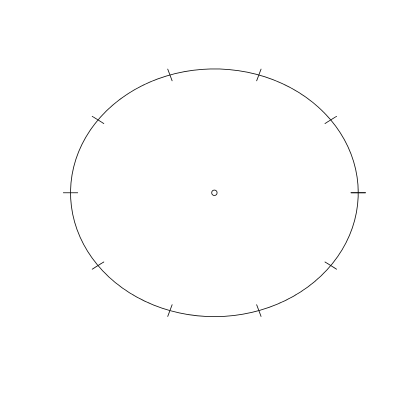
\includegraphics[width=4in, height = 4.2in]{../plots/spinnerCircle.png}
 % png("plots/spinnerCircle.png",height=400,width=400)
 % myValues <- seq(0, 2.01*pi, length = 100)
 % plot(cos(myValues),sin(myValues), type = "l", xlab = "", ylab = "", axes=FALSE, bty="n")
 % ticks <- 0:10 * pi/5
 % segments(.95*cos(ticks), .95*sin(ticks), 1.05*cos(ticks),  1.05*sin(ticks))
 % points(0,0)       ## abline(h=0); abline(v=0)
 % dev.off()
\vspace{-1cm}

  \item Now we'll use a web app to speed up the process.  Go to
     \webAppURLFrst and click \fbox{Test/Estimate} under the \fbox{One
       Categ} menu. 
       Enter the counts to show how many Linzmayer got right and got
       wrong. (These should add up to 25, but neither is 25.)
       Click ``Use These Data'' and record his proportion correct.

\begin{students}
  \vspace{1cm}
\end{students}
\begin{key}
{\it $\phat = 0.36$}
\end{key}

   \item Now  choose \fbox{Test}. and enter
     the value from \ref{trueESP-p} as the True Proportion.   Run 5000
     or more samples  and sketch the plot below.
\begin{students}
  \vspace{2cm}
\end{students}

\begin{key}
  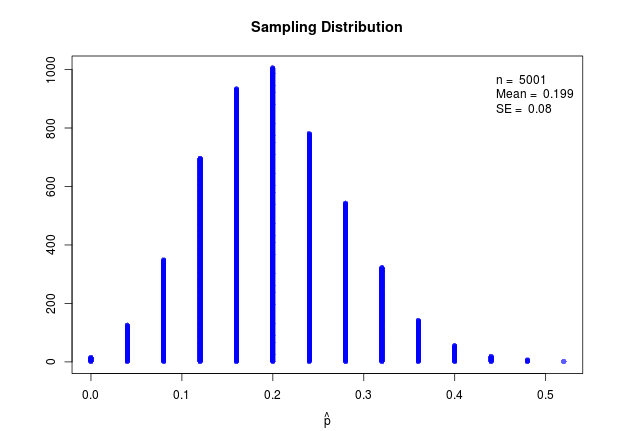
\includegraphics[width = .5\linewidth]{../plots/ESP-5001Draws.png}
\end{key}

     \item Check the summary statistics inside the plotting window.
       Does the mean agree with the null or alternative hypothesis?
       Explain why it should.
\begin{students}
  \vspace{1.2cm}
\end{students}
\begin{key}
{\it My mean is 0.199, which is darn close to 0.20. They should agree
  because the simulations were created by assuming $H_0$ is true.}
\end{key}
\\

     \item What proportion did Linzmayer get correct? \\
           Type that value in to the box just after ``than'' below the
           plot.  Select the direction (less, more extreme, or greater)
           based on the alternative hypothesis in
           \ref{ESP-hyps}. Click \fbox{Go} and record the proportion of
           times this occurred.\\  
           Would you consider this an unlikely result?
\begin{students}
  \vspace{1.2cm}
\end{students}
\begin{key}
{\it $\phat = 0.36$, I got 226 results of 5001 that
  were this extreme (p-value = 0.045), so doing this well is pretty unlikely.}
\end{key}
\\

     \item  Go back to figure \ref{fig:SOE-pvalue} on page
       \pageref{fig:SOE-pvalue}  to report the
       strength of evidence against $H_0$.  Give the numeric value and a
       verbal description of the strength of evidence.  
\begin{students}
  \vspace{1cm}
\end{students}
\begin{key}
{\it The p-value we observed is 0.045, which gives ``moderately
  strong'' evidence against $H_0$. }
\end{key}
\\
\end{enumerate}



% {\bf 3S Strategy for Measuring Strength of Evidence}\vspace{-.4cm}
% \begin{enumerate}
% \item  Statistic: Compute the statistic from the observed sample data. 
% \item  Simulate: Identify a ``by chance alone'' explanation for the
%   data. Repeatedly simulate values of the statistic that could have
%   happened when the chance model is true. 
% \item  Strength of evidence: Consider whether the value of the
%   observed statistic from the research study is unlikely to occur if
%   the chance model is true. If we decide the observed statistic is
%   unlikely to occur by chance alone, then we can conclude that the
%   observed data provide strong evidence against the plausibility of
%   the chance model. If not, then we consider the chance model to be a
%   plausible (believable) explanation for the observed data; in other
%   words what we observed could plausibly have happened just by random
%   chance. 
% \end{enumerate}


% Let’s review how we have already applied the 3S strategy to this study.
% \begin{enumerate}
% \setcounter{enumi}{17}
% \item Statistic. What is the statistic in this study?\vspace{.62cm} 
% \item  Simulate. Describe the three inputs we had to give the web app
%   and the results it returned. \vspace{2cm} 
% \item  Strength of evidence. What feature of the app's output gave the
%   p--value? \vspace{2cm} 

% \end{enumerate}

{\bf Step 5: Formulate conclusions.}\\
 Based on this analysis, do you believe  that Linzmayer was just
 guessing? Why or why not? 

\begin{students}
  \vspace{1.5cm}
\end{students}
\begin{key}
{\it This is fairly strong evidence that he was not just guessing.}
\end{key}

Are there ways other than ESP that a person could do well as a ``receiver''?
Explain. 

\begin{students}
  \vspace{1cm}
\end{students}
\begin{key}
{\it Yes, he could be cheating in some way.}
\end{key}


Another part of the scientific method is a reliance on replication.
Other scientists tried to replicate this study and could not find
another person like Linzmayer. 



{\bf Take Home Messages}\vspace{-.5cm}
\begin{itemize}
\item 
This activity was much like the previous one (Helper--Hinderer),
except that the null hypothesis value was not one-half. (Here ``at
random'' was 1 of 5, not 1 of 2)
\item 
Again note how $H_0$ is used to compute the p--value.  The alternative
comes into play only when we need to see which direction to count as
``more extreme''.
\item 
Both examples we've done so far have used a $>$ alternative, but that
is not always the case.
\item 
And finally: other reporting on Linzmayer suggests that he was
cheating, rather than reading minds.
 \item 
  Use the Notes page for any questions or your own summary of the
  lesson. \\
  
\end{itemize}

\noindent
{\bf Assignment}\vspace{-.5cm}
\begin{itemize}
%\item  D2Box 2 is due Jan 28.
\item 
%{\bf D2Quiz 3} is due Feb 1. Do it online. Recall, you can
%  save and keep working on it, but once you submit, it's gone.\\
  We strongly encourage you to get help in the Math Learning Center.
\item Watch videos assigned on D2L   
\item Read the next two pages.
\end{itemize}





  %% ESP   pgs 45 - 48
 \newpage

\fancyhead[LE,RO]{
   {\it Notes }\\
   {\it Unit \unitNum\   \ Page \thepage }
}
%Intentionally left blank
\phantom{No text here}
\newpage


\fancyhead[LE,RO]{
   {\it \theTopic }\\
   {\it Unit \unitNum\   \ Page \thepage }
}
  \def\theTopic{Reading 5}

\section{Do rats feel for others?}

Title:  ``Empathy and Pro-Social Behavior in Rats''

Authors: Inbal Ben-Ami Bartal, Jean Decety, Peggy Mason

Journal: {\it Science} {\bf 9} December 2011: Vol. 334 no. 6061 pp. 1427-1430 

ABSTRACT\\
\begin{quotation}
  Whereas human pro-social behavior is often driven by empathic concern
for another, it is unclear whether nonprimate mammals experience a
similar motivational state. To test for empathically motivated
pro-social behavior in rodents, we placed a free rat in an arena with
a cagemate trapped in a restrainer. After several sessions, the free
rat learned to intentionally and quickly open the restrainer and free
the cagemate. Rats did not open empty or object-containing
restrainers. They freed cagemates even when social contact was
prevented. When liberating a cagemate was pitted against chocolate
contained within a second restrainer, rats opened both restrainers and
typically shared the chocolate. Thus, rats behave pro-socially in
response to a conspecific’s distress, providing strong evidence for
biological roots of empathically motivated helping behavior. 
\end{quotation}

Watch this video:\\
\url{http://video.sciencemag.org/VideoLab/1310979895001/1/psychology}\vfill

Questions:
\begin{itemize}
\item What simple example of ``emotional contagion'' is mentioned? \vfill
 %  one baby cries -> all cry
\item What was the free rat's immediate reaction after first opening
  the cage door?  \vfill
\item What did both rats do when the caged rat was freed? (the first
  time). \vfill
\item How did the free rat's reaction change as it got used to the
  setup?  \vfill
\item Did the free rat open cages that contained:
  \begin{itemize}
  \item chocolates
  \item a toy rat
  \item nothing \vfill
  \end{itemize}
\item What does Peggy Mason conclude is ``in our brain''?\vspace*{\fill}
\end{itemize}
 %% p 49- 50 buff
  \newpage

\fancyhead[LE,RO]{
   {\it \theTopic }\\
   {\it Unit \unitNum\  Activity \dayNum \ Page \thepage } 
}
 
\def\theTopic{Interval Estimate }
\def\dayNum{6}

\section{ Interval Estimate for a Proportion}


If we call someone a ``rat'', we don't mean that they are nice to be
around, but rats might not deserve their bad reputation. Researchers
examining rat's capacity for empathy designed a study in which a pair
of rats were placed in the same cage.  One was trapped in a cramped
inner cage, while the other could move around much more, and could
also free the trapped rat if it chose to do so.  Of thirty pairs of
rats in the experiment, 23 of the free rats released the trapped
rat even though they then had to share the available food.

%% and 5 of 40 controls

\begin{center}
  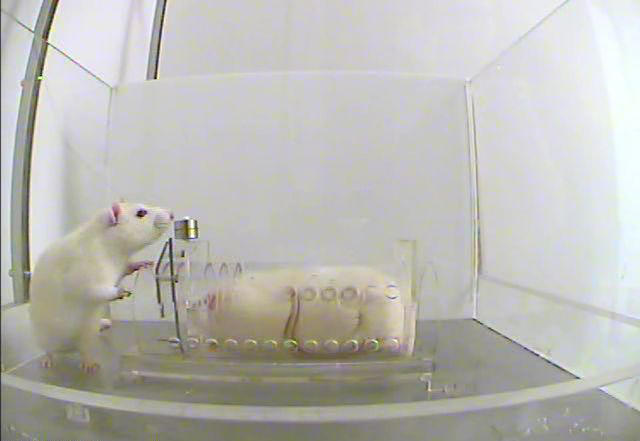
\includegraphics[width=.4\linewidth]{../plots/trappedRat.png}
\end{center}

The lab rats  used in the study are genetically identical to other
rats of the same strain, and can be assumed to be a ``representative
sample'' from the population of all rats of this strain.  Researchers
need a good estimate of the true proportion of these rats who would
free another rat trapped in the inner cage.

{\sf Step 1. State the research question.}\vspace{-.1in}
\begin{enumerate}
  \item Based on the description of the study, state the researcher's
   need as a question. 
\begin{students}
  \vspace{1cm}
\end{students}

\begin{key}
{\it How large is the proportion of rats of this strain who show
  ``compassion'' to a trapped rat?}
\end{key}

\end{enumerate}


{\sf Step 2. Design a study and collect data.}\vspace{-.1in}
\begin{enumerate}
  \setcounter{enumi}{1}
  \item \label{RatOptions} What actions of the free rat will be recorded? 
\begin{students}
  \vspace{1cm}
\end{students}

\begin{key}
{\it Free the trapped rat or leave it caged.}
\end{key}

  \item Your answer above gives the outcomes of the  variable of interest in the study.  Is this variable quantitative or categorical?
\begin{students}
  \vspace{1cm}
\end{students}

\begin{key}
{\it  categorical}
\end{key}

  \item  What is the parameter the researchers were interested in?
    Describe it in words and use proper notation to denote it. 
\begin{students}
  \vspace{1cm}
\end{students}

\begin{key}
{\it  $p$, the true proportion of rats of this strain who will free
  a fellow trapped rat.}
\end{key}
\end{enumerate}


{\sf Step 3. Explore and summarize the data.}\vspace{-.1in}
\begin{enumerate}
  \setcounter{enumi}{4}
  \item What is the sample size in this study?  $n = $
\begin{students}
  \vspace{1cm}
\end{students}
\begin{key}
{\it  30}
\end{key}

  \item \label{p.hat} Determine the observed statistic and use correct
    notation to  denote it.
\begin{students}
  \vspace{1cm}
\end{students}

\begin{key}
{\it  $\widehat{p} = 23/30 = 0.7667$}
\end{key}

  \item If the experiment were repeated with another 30 pairs of rats,
    do you think you would get exactly 23 who opened the cage again?
    Explain. 
\begin{students}
  \vspace{2.5cm}
\end{students}

\begin{key}
{\it  Not exactly, A few more or less than 23 would free the trapped
  rat. }
\end{key}
\end{enumerate}



{\sf Step 4. Draw inferences beyond the data. }\\

  The previous point is simple, but really important. When we repeat the
  same experiment, we do not get exactly the same results.   Why is
  that?  (Yes, you need to write an answer right here!  The future of
  the world -- no, I mean your success in this course -- depends on it.) 
\begin{students}
  \vspace{2.5cm}
\end{students}

\begin{key}
{\it  Rats differ from each other. We've seen that not all 30 rats
  make the same choice, so if we randomly grab another 30 rats, we
  expect either fewer or more to release the captives, not always 23. }
\end{key}


  We know exactly what proportion of rats in the sample showed
  empathy, and that number makes a good estimate of the same
  proportion of empathetic rats in the population.  However, the fact
  that not all rats, and not all samples are the same tells us we need
  to expect some variation in our sample proportion when we repeat the
  experiment. 

  A single number like the one you computed in
  \ref{p.hat} does not tell the whole story.  We want to let our
  reader know ``how good'' this estimate is.  One way to report the
  quality of an estimate is to give a range of values -- an interval
  estimate --  instead of a  single ``point estimate''.  

  Because we now have easy access to computers, we can run a {\bf
    simulation} to see how variable the statistic might be.  We only
  get one sample of real data, but we can create lots of simulated
  datasets which represent other values which might have been observed.

\begin{enumerate}
  \setcounter{enumi}{7}
\item \label{cards} Your group will get 30 cards on which you will
  write (or check that the previous class properly wrote) the
  observed outcomes from (\ref{RatOptions}) -- one for each of the 30
  pairs. We don't care about order, just that we get the right
  numbers of cards for each outcome.  Next we simulate another experiment on
  another sample of 30 rat pairs.  We can't actually get more rats and
  study them, so we ``recycle'' the numbers we have.
  \begin{enumerate}
  \item Shuffle your cards and draw one at random. Record the outcome
    for this pair.\\
  \item Replace the card into the deck, shuffle and draw a new card.
    This is a simple but powerful
    idea.  By sampling {\bf with replacement} we have the same
    conditions for every draw, and the probability of each outcome
    stays the same.  Record your second outcome.\\
  \item Repeat until you have 30 outcomes chosen at random.  What
    proportion of your rats were freed? \vspace{1cm}
  \end{enumerate}

  The process you just used is called {\bf bootstrapping} (which means
  to make something out of little or nothing), and the 30 outcomes are called a
  bootstrap {\bf resample}.  It's not a sample -- we only get one of
  those -- whereas we can repeat the resampling process many times.

  After collecting many resampled statistics, we'll use the
  {\bf percentile method} to compute a confidence interval.

  \item Reshuffling is slow, so we want to speed up the
    process by using the computer.  Our goal is to see what other
    outcomes we might have gotten for different samples of 30 rat
    pairs. We will again use  \fbox{Test or Estimate} under the
    \fbox{One Categ.} header in the  web app at
    \webAppURLFrst .
    Enter    the rat data to look like:\\
    \begin{tabular}{lr}
      \fbox{Freed}& \fbox{\  23\  }\\
      \fbox{Not} & \fbox{\  7 \  }
    \end{tabular}

    Then choose  \fbox{Estimate}. 
    What proportion of the rats were freed in your first resample?
    (Click the blue dot to see the resample.)
\begin{students}
  \vspace{1cm}
\end{students}

\begin{key}
{\it  AWV}
\end{key}

 \item Now resample several 1000 times and copy the picture you get here.
\begin{students}
  \vspace{4cm}
\end{students}

\begin{key}
  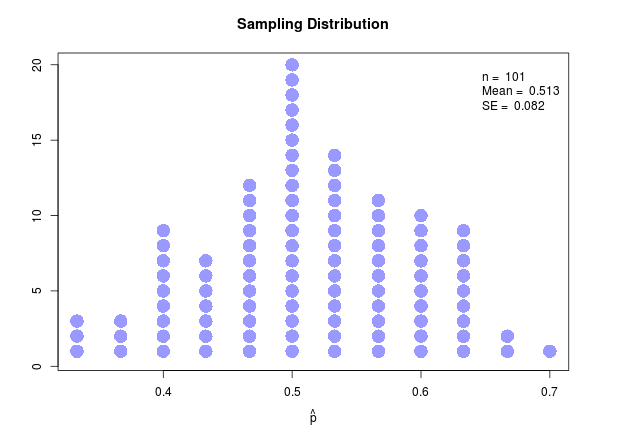
\includegraphics[width=.5\linewidth]{../plots/freeRats-101resamples.png}
\end{key} 

   Where is the distribution centered? (We are looking at the
   distribution of resampled $\phat$'s. The values in the corner of
   the plot are the mean and standard deviation of all blue dot values.) 
\begin{students}
  \vspace{.6cm}
\end{students}

\begin{key}
{\it  approx 0.77}
\end{key}

   How spread out are the sample outcomes? (SE stands for  standard
    error, which is the standard deviation of the resampled values.)
\begin{students}
  \vspace{.6cm}
\end{students}

\begin{key}
{\it  approx 0.078}
\end{key}

 \item The center should seem reasonable.  Why is the distribution
   centered at this value?
\begin{students}
  \vspace{1cm}
\end{students}

\begin{key}
{\it  The simulation is run assuming rats are freed with probability 0.77.}
\end{key}


 \item You should have several thousand blue dots and the plot should have
   stabilized so that adding another 1000 doesn't change the shape much.
   Below the plot we have options for confidence limits for our
   interval estimate.
   \begin{enumerate}
   \item Click \fbox{80} and count:   What proportion are red points
     in the left tail? 
\begin{key}
{\it  $N/10$}
\end{key}
     \\
      What proportion are red points in the right tail?
\begin{key}
{\it  $N/10$}
\end{key}
     \\
      What proportion are red points in the  middle?  \hfill Write the interval:
\begin{key}
{\it  80\}
\end{key}
     \\
   \item Click \fbox{90} and estimate: What proportion are red points in the left tail?
\begin{key}
{\it  5\%}
\end{key}
     \\
      What proportion are reds in the right tail?
\begin{key}
{\it  5\%}
\end{key}
     \\
      What proportion are blue points in the middle? \hfill Write the interval:
\begin{key}
{\it  91}
\end{key}
     \\
  \item Click \fbox{95} and count:   What proportion are red points in the left tail?
\begin{key}
{\it  3}
\end{key}
     \\
      What proportion are reds in the right tail?
\begin{key}
{\it  3}
\end{key}
     \\
      What proportion are blue points in the middle? \hfill Write the interval:
\begin{key}
{\it  95}
\end{key}
     \\
   \item Explain how the confidence limit is related to the number of
     blue points.
\begin{students}
  \vspace{1cm}
\end{students}

\begin{key}
{\it  With $N$ points, the percentage coverage matches the proportion of
  points left as blue in the middle.}
\end{key}


   \item Play with the ``Confidence Limit'' buttons more to explain:
    How are the endpoints of the interval estimate related to the
    colors of the points in the plot?\begin{students}
  \vspace{.8cm}
\end{students}

\begin{key}
{\it The endpoints are the values at which colors change from red to
blue or vice versa.}
\end{key}

  \item Predict: what will happen to the interval endpoints of
    a 90 \% interval, if we go from 5000 to 10000 resamples?
\begin{students}
  \vspace{.8cm}
\end{students}

\begin{key}
{\it  Tail counts should double, percentages stay the same; only
  slight change in interval endpoints.}
\end{key}

  \item Try it and see: were you right?
\begin{students}
  \vspace{.4cm}
\end{students}
    \end{enumerate}

  \item We need to spend more time on the meaning of ``Confidence'',
    but first let's review:  Explain
   how one dot in the plot was created.  (I suggest going back to how
   you did it manually in \ref{cards}.)
\begin{students}
  \vspace{6cm}
\end{students}

\begin{key}
{\it  We resampled from 30 cards containing 23 ``freed'' and 7 ``not
  freed'' values 30 times.  For each draw, record which type of card
  we get. Compute the proportion of ``freed'' rats in this resample. }
\end{key}
    
 \end{enumerate}


\begin{center}
  {\large \bf Take Home Message} \vspace{-.5cm}
\end{center}

Several very BIG ideas:\vspace{-.8cm}
\begin{itemize}
\item We only get one sample, but we can create many ``resamples''
  using sampling with replacement (also called bootstrapping).\\
  Because we are estimating (not assuming a null value), we must
  sample {\bf with replacement} to make each point come from the same
  distribution.  

\item Interval estimates are better than point estimates.
  \begin{itemize}
  \item They don't pretend to be exact. Any exact value is almost
    certainly wrong.
  \item By looking at the width of an interval we can evaluate the
    quality of the data.  Wide intervals are not very useful.  Skinny
    intervals are more informative.
  \item We can pretend that we know the true value of a parameter in
    order to test our methods.
  \item Our methods are not ``fail safe'', but are actually designed
    to have a certain error rate, for example, 5\% of the time our
    95\% confidence intervals will fail to cover the true parameter.
  \end{itemize}
% \item Our confidence in a particular interval is actually in the
%   process used to create the interval.  We know that using this
%   process over and over again (go out and collect a new random sample
%   for each time) gives intervals which will usually
%   cover the true value.\\
%    We cannot know if a particular interval covered or not, so you have
%    to be tolerant of some uncertainty.  We will explore this more in
%    your next class period.
 \item 
  Any questions? \vfill
\end{itemize}


\noindent
{\bf Assignment}\vspace{-.5cm}
\begin{itemize}
%\item   D2Quiz 3 due Feb 1.
%\item {\bf D2Box 3} is due Feb 4th. Turn in as a pdf file to the D2L drop box.
%  We strongly encourage you to get help in the Math Learning Center.
 \item Watch videos  \# 7 and 8  before the next class.
\item Fill in the simulation confidence interval box in column 1 of
  the Review Table.

\item Read  the  next reading.
\end{itemize}






  %% Rats - CI   pgs 51 - 56
 \newpage


\fancyhead[LE,RO]{
   {\it Notes }\\
   {\it Unit \unitNum\   \ Page \thepage }
}
%Intentionally left blank
\phantom{No text here}
\newpage

    

\fancyhead[LE,RO]{
   {\it \theTopic }\\
   {\it Unit \unitNum\   \ Page \thepage }
}
  \def\theTopic{Reading 6}

\section { What Does ``Confidence'' Mean?}

Mark Twain said:
\begin{quotation}
All you need in this life is ignorance and confidence, and then
success is sure.   
\end{quotation}

 from quarterback Joe Namath:
\begin{quotation}
When you have confidence, you can have a lot of fun. And when you have fun, you can do amazing things.  
\end{quotation}

and from scientist Marie Curie:
\begin{quotation}
  Life is not easy for any of us. But what of that? We must have
  perseverance and above all confidence in ourselves. We must believe
  that we are gifted for something and that this thing must be
  attained. 
\end{quotation}

The above quotes (from brainyquote.com) refer to  ``self confidence''
which is certainly important in any endeavor.
In statistics, the word ``confidence'' is best summarized as {\bf
  faith in the process} by which an estimate (in our case, an interval
estimate) was created.  A confidence interval carries information
about the {\bf location} of the parameter of interest, and tells us a lot
about the {\bf precision} of the estimate through the interval
length. 


In the news, interval estimates are often reported as a point value
and a {\bf margin of error}. 

\begin{quotation}
  71\% of Democrats and independents who lean to the Democratic Party
  say the Earth is warming due to human activity, compared with 27\%
  among their Republican counterparts (a difference of 44 percentage
  points). This report shows that these differences hold even when
  taking into account the differing characteristics of Democrats and
  Republicans, such as their different age and racial profiles. 
\end{quotation}

  Read the explanation from the  Pew Research Center  of how they
  conducted the poll,
\url{http://www.pewinternet.org/2015/07/01/appendix-a-about-the-general-public-survey-2/}.
 The margin of error they give is for what confidence level?
  \vfill

 How large is the margin of error for Republican/lean Republican?
\begin{students}
\vspace{.8cm}
\end{students}

\begin{key}
  {\em 5.1\%}
\end{key}

 For  Democrat/lean Democrat?
\begin{students}
\vspace{.8cm}
\end{students}

\begin{key}
  {\em 4.5\%}
\end{key}

\newpage

\subsection{ Plus or Minus Confidence Intervals}


In the web app used in previous activities, we clicked on a confidence
level and the web app colored in the right number of dots as red to
put our selected percentage of sampled proportions in the center
(these stayed blue) and split the remainder into the two tails,
turning these more extreme points red.  We call this a ``percentile''
method because, for example, a 90\% CI has lower endpoint of the 5th
percentile and upper endpoint of the 95th percentile.

Another common way of building a 95\% confidence interval is to take
the estimated value and add and subtract twice the standard error of
the statistic.  A 95\% confidence interval for $p$ is then
 $$ \phat \pm 2 SE(\phat)$$
where $SE(\phat)$ is a number coming from the plot on the web app.
Why 2?  Well, it's easy to remember, and with a symmetric
distribution, 95\% of the data will fall within 2 SD's (standard
deviations) of the mean.

Margin of error is then the amount we add and subtract.  In this case,
it is twice $SE(\phat)$.  (Note: the parentheses do not mean
multiplication, say of SE times $\phat$. They indicate that $SE$ is a
function of $\phat$, in the same way we use $\log(x)$ or
$\sin(\theta)$.)\\
Open the web app: \webAppURLFrst .

\begin{enumerate}
\item Go back to the rat data from Activity 6 where 23 rats opened the
  cage and 7 did not.  Reenter the data in the \fbox{One Categ} part
  of the web app, and select \fbox{Estimate}. 
  \begin{enumerate}
  \item Generate 5000 to 10,000 resamples and click 95\%. Record the
    interval here:
\begin{students}
\vspace{1.5cm}
\end{students}

\begin{key}
  {\em (0.60, 0.90)}
\end{key}
\item Now write down the SE shown near the top right corner of the
  plot.  (We will not use the mean of the plotted values).
\begin{students}
\vspace{1.5cm}
\end{students}

\begin{key}
  {\em 0.077}
\end{key}
\item Add and subtract $2SE$ from the original proportion given in the
  box at left ( {\bf Do not} use the mean from the plot.) and write it
  in interval notation.

\begin{students}
\vspace{1.5cm}
\end{students}

\begin{key}
  {$ 0.77 \pm 2\times 0.077 =  (0.63, 0.91)$}
\end{key}
\item Compare the two intervals.  Is one wider? Is there a shift?

\begin{students}
\vspace{1.5cm}
\end{students}

\begin{key}
  {\em The percentile CI is shifted slightly to the left and is
    slightly wider.}
\end{key}

  \end{enumerate}
\end{enumerate}
 %% p 57- 58 buff
  \newpage
  
\fancyhead[LE,RO]{ 
   {\it \theTopic }\\
   {\it Unit \unitNum\  Activity \dayNum \ Page \thepage }
}
 
\def\theTopic{Confidence }
\def\dayNum{7}


\section{ Meaning of ``Confidence'' -- Activity}

To understand the meaning of the term ``confidence'', you have to step
back from the data at hand and look at the process we use to create
the interval.
\begin{itemize}
  \item Select a random sample from a population, measure each unit,
    and compute a  statistic like $\phat$ from it.
  \item Resample based on the statistic to create the interval.
  \end{itemize}

  \begin{center}
    {\large \bf Simulation}
  \end{center}

To check to see how well the techniques work, we have to take a
 special case where we actually know the true parameter value.
 Obviously, if we know the value, we don't need to estimate it, but we
 have another purpose in mind: we will use the true value to generate
 many samples, then use each sample to estimate the parameter, and
 finally, we can check to see how well the confidence interval
 procedure worked by looking at the proportion of intervals which
 succeed in capturing the parameter value we started with.

 Again go to \webAppURLFrst \ 
 and select \\
  \fbox{Confidence Interval Demo} from the \fbox{One Categ} menu.
 
 The first slider on this page allows us to set the sample size --
 like the number of units or subjects in the experiment.  Let's start with
 \fbox{40}.\\
 The second slider sets the true proportion of successes for each
 trial or spin (one trial).  Let's set that at \fbox{0.75} or 75\%
 which is close to the observed $\phat$ of the rat study.\\
 You can then choose the number of times to repeat the process -- gather
 new data and build a confidence interval: (10, 100, 1000 or 10K
 times) and the level of confidence you want (80, 90, 95, or 99\%). 
 We'll start with \fbox{100} simulations of a \fbox{90}\% CI.

  The upper plot shows 100  $\phat$'s -- one from each of the 100 simulations.
  \\
  The second plot shows the interval estimate we get from each
  $\phat$.  These  are stacked up to put smallest estimates on the
  bottom, largest on top. The vertical axis has no real meaning. 

  \begin{enumerate}
      \item   Click on a point in the first plot to see its corresponding CI in
  the second plot.  Especially try the largest and smallest points.
  Which intervals do they create (in terms of left or right position)?
\begin{students}
  \vspace{1cm}
\end{students}
\begin{key}
  {\it lowest and highest CI's, resp.}
\end{key}
\item How does the center of the green (or red)  interval relate to the $\phat$
  you've clicked?  
\begin{students}
  \vspace{1cm}
\end{students}
\begin{key}
  {\it It's the center}
\end{key}
\item There is a light gray vertical line in the center of the lower
  plot. What is the value (on the $x$ axis) for this plot and why is
  it marked?
\begin{students}
  \vspace{1cm}
\end{students}
\begin{key}
  {\it It is the true parameter value: 0.75 if you followed the directions.}
\end{key}
\item What color are the intervals which do not cross the vertical
  line? \\How many are there?
\begin{students}
  \vspace{1cm}
\end{students}

\begin{key}
  {\it red, AWV about 10}
\end{key}

\item What color are the intervals which cross over the vertical
  line? \\How many are there?
\begin{students}
  \vspace{1cm}
\end{students}

\begin{key}
  {\it green, AWV about 90}
\end{key}

\item Change the confidence level to \fbox{95}\%. Does the upper plot
  change?  Does the lower plot?  Describe any changes.
\begin{students}
  \vspace{1cm}
\end{students}
\begin{key}
  {\it Upper plot should not change. Each interval in the lower plot
    gets longer, so some that were red may turn green now.}
\end{key}


\item If you want an interval which is stronger for confidence
  (has a higher level), what will happen to its width?
\begin{students}
  \vspace{.6cm}
\end{students}
\begin{key}
  {\it it must be wider}
\end{key}

  \item Go up to 1000 or more intervals, try each confidence level in
    turn and record the coverage rate   (under plot 2) for each.\\
    \begin{tabular}{|r|r|r|r|} \hline
      {\large 80} &  {\large 90} &  {\large 95} &  {\large 99}\\ \hline
   {\large  \phantom{90000} } & {\large \phantom{90000}  } &  {\large
     \phantom{90000} } &  {\large  \phantom{90000} } \\
       & & & \\ \hline
    \end{tabular}


    \begin{center}
      {\large\bf Data Analysis}
    \end{center}
  \item Now back to the Pew study you read about for today. Of the 2002 people
    they contacted, 737 were classified as Republican (or Independents
    voting Rep) voters and 959 as Democrats (or Indep leaning Dem).
    \begin{enumerate}
    \item What integer number is closest to 27\% of the Republicans?
      Enter that value as the first count  in the \fbox{Test or
        Estimate} option under the \fbox{One Categ} menu   and the balance
      of those 737 in the bottom box. Relabel the
      categories, then click \fbox{Use These Data}  Check that the
      proportion on the summary page is  close to 0.27. 
      \begin{enumerate}
      \item What is your proportion of Republicans who think global
        warming is caused by human activity?
\begin{students}
\vspace{.8cm}
\end{students}

\begin{key}
  {\em 199 ``successes'', 538 ``Failures'', $\phat = $0.27}
\end{key}
      \item Click \fbox{Estimate}  and run several 1000
        samples. What is the SE?
\begin{students}
\vspace{.8cm}
\end{students}

\begin{key}
  {\em 0.016}
\end{key}
      \item Find the ``margin of error'' for a 95\% Confidence
        interval and create the interval.

\begin{students}
\vspace{.8cm}
\end{students}

\begin{key}
  {\em ME = 0.032, 95\% CI: 0.27$\pm 0.032 = (0.38, 0.302)$}
\end{key}
  \item Are the endpoints close to those we get from the web app?
\begin{students}
\vspace{.8cm}
\end{students}

\begin{key}
  {\em almost identical: ( 0.237 , 0.303 )}
\end{key}
      \end{enumerate}
    \item Repeat for the Democrats:
      \begin{enumerate}
      \item Numbers of ``successes'' and ``failures''.
\begin{students}
\vspace{.8cm}
\end{students}

\begin{key}
  {\em 700, 259 }
\end{key}
      \item Margin of error and 95\% CI related to it.
\begin{students}
\vspace{.8cm}
\end{students}

\begin{key}
  {\em 0.028, (0.702, 0.758)}
\end{key}
      \item Percentile interval and comparison.
\begin{students}
\vspace{.8cm}
\end{students}

\begin{key}
  {\em (0.701, 0.758), again very close. }
\end{key}
      \end{enumerate}
    \item Explain what we mean by ``confidence'' in these intervals we
      created.
\begin{students}
\vspace{3.8cm}
\end{students}

\begin{key}
  {\em We are 95\% confident that the true }
\end{key}

\item What can we say about the proportion of Republicans and the
  proportion of Democrats on this issue? Is it conceivable that the
  overall proportion is the same?  Explain.
\begin{students}
\\ \vspace{1cm}
\end{students}
\begin{key}
  {\em The intervals do not come close to overlapping, so we have to
    think that there is a strong difference of opinion between these
    two groups. I am ``quite confident'' of that.}
\end{key}
    \end{enumerate}
  \end{enumerate}

\begin{center}
  {\large \bf Take Home Message \vspace{-.2in}} 
\end{center}

\begin{itemize}
\item Interval estimates are better than point estimates.
\item Our confidence in a particular interval is actually in the
  process used to create the interval.  We know that using this
  process over and over again (go out and collect a new random sample
  for each time) gives intervals which will usually
  cover the true value.\\
   We cannot know if a particular interval covered or not, so we have
   to  tolerate some uncertainty.
 % \item 
 %  Any questions? How would you  summarize this  lesson?
\end{itemize}





\noindent
{\bf Assignment}
\begin{itemize}
%\item D2Box 3 is due Feb 4.
%\item {\bf D2Quiz 4} is due Feb 8. Do it online. Recall, you can
%  save and keep working on it, but once you submit, it's gone.
%%  We strongly encourage you to get help in the Math Learning Center.
\item Watch videos assigned on D2L   
\item Read the next two pages.
\end{itemize}

  %%  CI - meaning   pgs 59- 62
 \newpage


\fancyhead[LE,RO]{
   {\it Notes }\\
   {\it Unit \unitNum\   \ Page \thepage }
}
%Intentionally left blank
\phantom{No text here}
\newpage


\fancyhead[LE,RO]{ 
   {\it \theTopic }\\
   {\it Unit \unitNum\   \ Page \thepage }
}
  \def\theTopic{Reading 9}

\section{ The Sampling Distribution}


 Statistical inference is based on simple ideas of random treatment
 assignment, random selection, and random sampling.   {\bf RANDOM} 
 means that the outcome we will get cannot be known, but the
 distribution of possible outcomes can be known. 


\subsection{ Sampling Distribution for $\phat$}

 Consider selecting a random sample of 100 people with season passes
 to a local ski run and asking if they snow board more than they ski.
 Our sample will produce a sample  proportion -- a number which we
 cannot know ahead of time.  We will only select 
 one sample, and will only get to see one sample proportion, but we
 can think about the process of random selection and consider all the
 sample proportions we might have obtained.  This is a powerful way to
 think abstractly about the random selection process:
 \begin{itemize}
 \item We observe one sample.
 \item What else might we have observed?
 \end{itemize}
  The {\bf sampling distribution} is a description of all possible
  outcomes and the probabilities of obtaining each outcome.  If, for
  example, actually 48.7\%  of season pass holders board, then we
  could use a spinner to simulate the sampling distribution and would
  get a picture like this:

  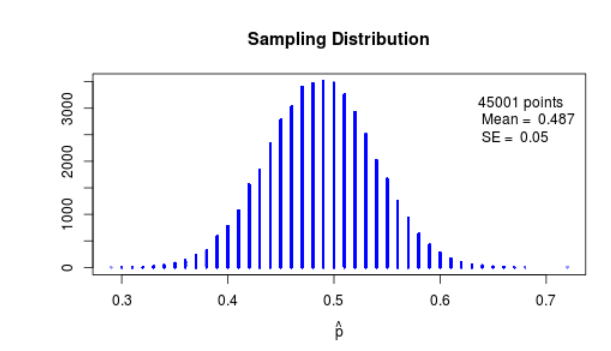
\includegraphics[width=.5\linewidth]{../plots/SampDistnofPhat-100.png}

It is centered at the true value, 0.487 as the proportion of boarders,
and has spread indicated by $SE(\phat) = 0.05$. 
%  If we decide to
% increase the sample size to 1000, the center will stay the same, but
% the spread will get smaller.
It would be very useful to know the sampling distribution so that we
could find the center part of the distribution for a confidence
interval.  

Sampling distribution for $\phat$ depends on two things: the true
parameter $p$ (unknown), and the sample size, $n$. As sample size
increases, spread gets smaller. \vspace{1in}

\subsection{ Sampling Distribution for $\xbar$}

 Now suppose we are interested in the average age of season pass
 holders in a sample of size 100. The sampling distribution  for the
 sample mean age, $\xbar$, 
 again depends on the  unknown parameter which is now $\mu$, the true
 mean age in the population,  and sample size, $n$,
 but it also depends on the spread in the original distribution,
 $\sigma$.  
 The left hand pair of plots below is for individual season pass
 holders created (not real data) under two different assumed values
 for spread, either $\sigma = 5.5$ or $\sigma = 8$.

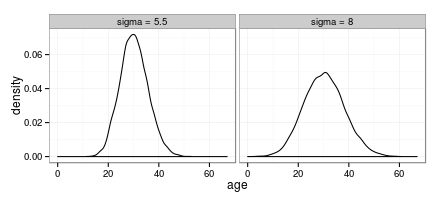
\includegraphics[width =.48\linewidth]{plots/twoSampDensities4x.png}
\hfill
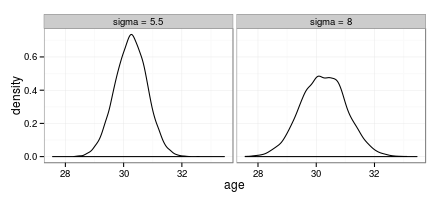
\includegraphics[width =.48\linewidth]{plots/twoSampDensities4xbar.png}\\

 The right hand pair of plots  shows the distributions of {\bf MEAN ages of 100
   season pass holders.} 

 A common confusion is to think that means will have the same
 distribution as the individuals. The two distributions will have the
 same centers, but when we average to get means, we pull in the
 extreme points.  The distribution on the right has more younger and
 older ages, but still, when averaged over 100 people (top plot) we
 rarely see a sample average as low as 28.

 Our point is that even though the distributions shown have the same
 means $\mu$, and the same $n =  100$ the different values for
 $\sigma$ change the sampling distributions for $\xbar$, the sample mean. 



 

{\bf Important Points}
\begin{itemize}
\item What does it mean to say that an outcome is ``random''?\vfill
\item Why does a plot of a sampling distribution show many points, not
  just one? After all, there is just one sample, right?\vfill
\item Sampling distributions of $\phat$ and of $\xbar$ both depend on:
  \vfill
\item Additionally, the sampling distribution for $\xbar$ depends
  on:\vfill
\item Why is the sampling distribution for $\xbar$ less spread out
  than the distribution of the original data?
\end{itemize}


%% R code
% require(ggplot2)
% sample1 <- apply(matrix(rpois(1000000,30.25), nrow=100),2,mean)
% sample2 <- apply(matrix(rpois(1000000,60.25)-30, nrow=100),2,mean)
%  sampMeanFrame <- data.frame(age = c(sample1, sample2), sample = gl(2,
%  10000, labels = c("sigma = 5.5", "sigma = 8")))
%  qplot( x = age,  facets =  ~ sample, data = sampMeanFrame, geom = "density") + theme_bw()
% dev.copy(png,file = "plots/twoSampDensities4xbar.png",height = 200,
% width = 440);dev.off()

%  sample1 <- rpois(10000,30.25)
%  sample2 <- rpois(10000,64.25)-34
%   sampXFrame <- data.frame(age = c(sample1, sample2), sample = gl(2,
%   10000, labels = c("sigma = 5.5", "sigma = 8")))
%   qplot( x = age,  facets =  ~ sample, data = sampXFrame, geom =
%   "density", adjust = 1)  + theme_bw()
%  dev.copy(png,file = "plots/twoSampDensities4x.png",height = 200, width = 440);dev.off()  %% p 63-64  buff
%%  Reordering for summer 2016 renumbered 9 as 7
  \newpage


\fancyhead[LE,RO]{
   {\it Notes }\\
   {\it Unit \unitNum\   \ Page \thepage }
}
%Intentionally left blank
\phantom{No text here}
\newpage


\fancyhead[LE,RO]{
   {\it \theTopic }\\
   {\it Unit \unitNum\  Activity \dayNum \ Page \thepage }
}
 \def\theTopic{Textbook Costs}
\def\dayNum{8 }
 %% was 11 in Spring 2016

\section{Bootstrap  Confidence Interval for $\mu$}


We would like to know how much the ``typical'' MSU students spends on
books each semester.  Is this a question we can answer by testing?
  We need an estimate, and as you now know, we like interval
estimates because they include some information about uncertainty.

So far, the tools we have for working with a mean have allowed us to
test a pre-specified value, not estimate an unknown parameter.
We have a point estimate: a sample mean, $\xb$, but we don't know how
variable it is because we don't know $\sigma$, the true standard
deviation of the data points. 

{\bf Problem}:\\
We need to know the sampling distribution to know how far away our
statistic might be from our parameter.  We know the sampling
distribution of $ \xb$ is centered at the population mean, $\mu$, and
we know some things about its spread and shape.   However, the sampling
distribution  of $\xb$ depends on the unknown parameters $\mu$ and $\sigma$. How
can we estimate $\mu$?  


{\bf Solution}:\\Use the ``Resampling'' or Bootstrap distribution as a
substitute for the unknown sampling distribution.
\vspace{-.2in}
\begin{center}
	{\bf\sf	We only draw {\bf one} sample from the population!}
\end{center}

Hang onto that idea, because we will use our one sample  in an almost
magical way to generate something very much like the sampling
distribution.   

% When a computer ``boots up'' it goes from a dead state with no
% electrons moving through it to a live state where it's ready to accept
% instruction.  The word ``boot'' comes from ``bootstrap'' and a silly
% tale about Baron Munchausen who got himself out of quicksand by
% pulling on his bootstraps.  In statistics our objective is to take our
% one sample and create many samples from it. That seems a bit
% impossible, but computer scientists figured how to make a computer
% boot up, and similarly, statisticians have figured out how to measure
% sampling variation when we have only a single sample. 

  A {\bf bootstrap resample} is the same size as the original data, and
  consists of data points from the original data.  The only difference
  is that the resampling is done ``with replacement'' so a bootstrap
  resample typically contains several replicates of some values and is
  missing other values completely.  We can repeat this process many
  times and store the statistics generated from each resample.  The
  result is a bootstrap distribution (or a resampling distribution)
  which can be used as a replacement for the unknown sampling
  distribution.  In particular, we can use the spread (standard error)
  of the bootstrapped sample statistics as a substitute for the spread
  (standard error) of our statistic.  

   

Go to  the applet:\\
\webAppURLFrst and 
select \fbox{Bootstrap Demo}under  \fbox{One Quant}.
\vspace{-.2in}
\begin{enumerate}
  \item  The counts shown are all the values in the ``population'', which
    are amounts (in 10's of dollars) stat students in a prior semester
    spent on textbooks.  We will pretend that this is the entire
    population in order to see how well our methods work.
    \begin{enumerate}
    \item  Click \fbox{Sample} and we'll get a random sample of size
      8 from this population.  The population then disappears because
      we never can observe an entire population. Some of your numbers
      might be the same, but they came from different individuals in
      the population.  Click \fbox{Get New Sample} at the bottom of
      the page, and you'll get a new sample.  How many samples do 
       we collect in one study?
\begin{students}
        \vspace{1cm}        
\end{students}
\begin{key}
   {\it AWV. just one. }
\end{key}
    \item  Click \fbox{1 Resample} and watch what happens. Click
      \fbox{slower} 1 or 2 times and watch it again.  What is this
      button doing?
\begin{students}
        \vspace{1cm}        
\end{students}
\begin{key}
   {\it It selects 8 values from the sample with replacement, pulls
    each down to the next line, and leaves a colored spot on each one
    it grabbed.  The resample then gets combined (averaged) to a
    single value and that is plotted on the dotplot scale.}
\end{key}
    \item  Slow it down to where you can answer these questions: For
      one resample, which of the original eight values got used more
      than once? which not at all?
\begin{students}
        \vspace{1cm}        
\end{students}
\begin{key}
   {\it AWV.}
\end{key}
    \item Get 8 cards from your instructor and write each of the 8 values in
      your sample on a card.  Create your own bootstrap resample to
      mimic what the computer does.  Which of these methods works?
      (Circle one.)
      \begin{enumerate}
      \item Select one card at random, leave it out, and select
        another card.  Continue until you use all the cards.
      \item Select one card at random and write down its
        value. Replace it, reshuffle, and select another.  Continue
        until you've written down eight  values. 
      \end{enumerate}
      % Explain which technique copies what the computer does when it
      % collects one resample.
\begin{students}
        \vspace{.2cm}        
\end{students}
\begin{key}
\ \  \\
  {\it The second -- sampling With Replacement is what we are doing
    on the computer. The first way always gives the same resample
    mean -- they just change order. The second lets the resample mean vary.}
\end{key}

\item What statistic are we interested in (from the sample)?  Compute
  it for the resample. 
\begin{students}
        \vspace{1cm}        
\end{students}
\begin{key}
  \\{\it mean, $\xb$, AWV}
\end{key}

\item  Click \fbox{100}  in the ``Many Resamples'' choices.
  \begin{enumerate}
  \item  Explain  what values are being plotted.  
\begin{students}
        \vspace{2cm}        
\end{students}
\begin{key}
  \\{\it It takes  100 resamples, computes the mean of
    each, and plots the 100 resample means. }
\end{key}
  \item A common quiz/exam question is ``What does one dot
    represent?''. Explain where the values came from and what
    statistic was computed to make one dot. 
\begin{students}
        \vspace{2.5cm}        
\end{students}
\begin{key}
  \\{\it One dot is the mean of one resample which was found by
    randomly selecting 8  values from the sample with replacement. We
    then average them     together.}
\end{key}
\end{enumerate}

\item  Click \fbox{500}  in the ``Many Resamples'' choices.
 Write down the interval estimate.  Count
      (approximately) how many circles are outside the red
      lines at the left and at the right.
\begin{students}
        \vspace{1cm}        
\end{students}
\begin{key}
  \\{\it (16.4, 55.4)  I see about 12 circles below and  12 above the interval.}
\end{key}
\\
  Repeat twice more. Write down each confidence interval and guess how
  many points fall outside each.
\begin{students}
        \vspace{1cm}        
\end{students}
\begin{key}
{\it AWV. I got (18.1, 54.9), (18.3, 54.9)}
\end{key}

\item Click  1000,  5000,and 10000 in turn. Write down
  three CI's for each.  Compare the CI's.  Are some groups off-center compared
  to others?  More variable?

\begin{students}
\vspace{4cm}
\end{students}
\begin{key}
  {\it The smaller numbers of resamples give more variability in
    CI. Centers don't change.}
\end{key}


\item Go back to 500 resamples.  What happens to length of intervals
  when we change confidence levels?  Hint: choose a different
  confidence level with the buttons, then click \fbox{500} again
  to obtain the interval.\\
\begin{students}
{\large \tt
\begin{tabular}{rc}
from 95\% to 99\% --	&	intervals  \underline{\hspace*{2in}}\\
from 95\% to 90\% --	&	intervals \underline{\hspace*{2in}}\\
\end{tabular}
}
\end{students}
\begin{key}
going from 95\% to 99\%  confidence 	intervals get longer\\
going from 95\% to 90\%  confidence 	intervals get shorter
\end{key}
    \end{enumerate}


\item When we started, we saw the whole population of counts
    which has true mean  $\mu = 34.5$ (\$345).
    \begin{enumerate}
    \item  Look back at the 90\% interval you wrote down. Did it
      contain the true value? Write ``Hit'' or ``Miss''.
\begin{students}
        \vspace{1cm}        
\end{students}
\begin{key}
  {\it AWV. All of mine did.}
\end{key}

\item  We'll now pretend that we can grab new samples and we will
  build two 90\% CI's from each as a check of consistency.
 For each row of the table, click \fbox{Get New Sample} once, then
 click \fbox{1000} to get a 90\% CI for $\mu$.  Record whether your
 first interval covers 34.5 (Hits) or not (Misses). Click  \fbox{1000}
 again, and write  ``missed'' or ``hit'' in the third column.\vspace{.5cm}\\
\begin{students}
  \begin{tabular}{l|c|c|c|}
   Click \fbox{New Sample} & \fbox{1000} Hit or Missed?&  \fbox{1000}
   Hit or Missed?& Same?\\ 
    \hline
1   \ \ & \ \ & \ \ & \ \\ 
   \ \ & \ \ & \ \ & \ \\   \hline
2   \ \ & \ \ & \ \ & \ \\ 
   \ \ & \ \ & \ \ & \ \\   \hline
3   \ \ & \ \ & \ \ & \ \\ 
   \ \ & \ \ & \ \ & \ \\   \hline
4   \ \ & \ \ & \ \ & \  \\ 
   \ \ & \ \ & \ \ & \ \\   \hline
5   \ \ & \ \ & \ \ & \  \\ 
   \ \ & \ \ & \ \ & \ \\   \hline
 \end{tabular}

  \begin{tabular}{l|c|c|c|}
   Click \fbox{New Sample} & \fbox{1000} Hit or Missed?&  \fbox{1000}
   Hit or Missed?& Same?\\ 
    \hline
6   \ \ & \ \ & \ \ & \  \\ 
   \ \ & \ \ & \ \ & \ \\   \hline
7   \ \ & \ \ & \ \ & \ \\ 
   \ \ & \ \ & \ \ & \ \\   \hline
8   \ \ & \ \ & \ \ & \ \\ 
   \ \ & \ \ & \ \ & \ \\   \hline
9   \ \ & \ \ & \ \ & \  \\ 
   \ \ & \ \ & \ \ & \  \\   \hline
10   \ \ & \ \ & \ \ & \  \\ 
   \ \ & \ \ & \ \ & \  \\   \hline
  \end{tabular}
\end{students}

   In each line above put a check in the last column if the 2
   intervals agreed (both hit or both missed). 
   Does coverage depend more on the sample or on the particular resample?

\begin{students}
        \vspace{2cm}        
\end{students}
\begin{key}
 {\it The sample.  This is just like the simulation we did for
    proportions, but the method for computing the confidence interval
    is different.  We can get a ``good'' or ``bad'' sample, but given
    the sample, the method is consistent.  }
\end{key}
\end{enumerate}
\item With proportions we used $\widehat{p} \pm 2 SE$ as our
  confidence interval.  For means, we have extra variation from not
  knowing the spread, $\sigma$, so the correct multiplier depends on
  sample size as well as confidence level.  For sample size $n=8$, the
  multiplier is $t_7^* = 2.36$ for 95\% confidence, 3.50 for 99\%
  confidence, and 1.89 for 90\% confidence.  The web app shows
  standard error of the resampled means as SD, so we use this as our
  SE.  Build 90, 95, and 99\% CI's using the $\xb \pm t^* SE$ method.
  Also write the bootstrap intervals to compare.\\
  \begin{enumerate} 
  \item Compute the mean of your sample (from the 8 values, not the
    ``Mean'' printed) \\ $\xb =$ 
\begin{key} 
 {\it AWV, mine is 24.125}
\end{key}
\item a 90\% CI for $\mu$ is (show work)
\begin{students}
        \vspace{1cm}        
\end{students}
\begin{key}
 {\it AWV, $24.125 \pm  1.89 \times 5.25 = (14.2, 34.1)$\\
     Bootstrap: (15.4, 32.5)}
\end{key}
\item a 95\% CI for $\mu$ is (show work)
\begin{students}
        \vspace{1cm}        
\end{students}
\begin{key}
 {\it AWV, $24.125 \pm  2.36 \times 5.39 = (11.4, 36.8)$\\
     Bootstrap: (13.8, 35)}
\end{key}
\item a 99\% CI for $\mu$ is (show work)
\begin{students}
        \vspace{1cm}        
\end{students}
\begin{key}
 {\it AWV, $24.125 \pm  3.50 \times 5.31 = ( 5.5, 42.7)$\\
     Bootstrap: (11.3, 36.9)}
\end{key}
\end{enumerate}
\item Is there a pattern when you compare the two methods?  Are
  bootstrap percentile methods always wider? shifted? relative to the 
 $\xb \pm t^* SE$ intervals?
\begin{students}
        \vspace{3cm}        
\end{students}
\begin{key}
  \\ {\it Bootstrap intervals are narrower.  There is a tendency for
    the $\xb \pm t^* SE$ intervals to be   too symmetric. }
\end{key}

\item Challenge: based on what you've seen so far in this course what
  will happen to our interval estimates if we 
  change  sample size from 8 to  4?  From 8 to 16?\\
   Will smaller sample size shift the center?
\begin{students}
        \vspace{.5cm}        \\
\end{students}
\begin{key}
{\it No, both are unbiased.}
\end{key}

Will smaller sample size change the width?
\begin{students}
        \vspace{.5cm}        
\end{students}
\begin{key}
\\{\it Yes, width should increase.}
\end{key}

   Will larger sample size shift the center?
\begin{students}
        \vspace{.5cm}        
\end{students}
\begin{key}
\\{\it No, both are unbiased.}
\end{key}

   Will larger sample size  change the width?\\
\begin{students}
        \vspace{.5cm}        
\end{students}
\begin{key}
\\ {\it Yes, width should shrink.}
\end{key}

   Try it and record what happens to center and spread.  (Yes, it is
   important to write it down. It will show up on the exam.)  Using
   just one sample may not give you a good comparison.  Try several
   samples at each sample size. 
   \vfill
\end{enumerate}

\begin{center}
  {\bf Take Home Messages}
\end{center}
\begin{itemize}
  \item   We only get one SAMPLE, but from it we can generate many
    resamples.
  \item We can use the resampling distribution to see how much
    samples vary. It is a substitute for the unknown sampling
    distribution.
  \item Whether the interval includes the parameter or not
    depends mainly on our luck in sampling.  Most samples give statistics
    close to the parameter, but some can be farther away.
  \item We can use the bootstrap information in two ways:
    \begin{itemize}
    \item to compute the SE of the statistic
    \item to find percentiles of the resampling distribution.
    \end{itemize}
   Either method can give a confidence interval.  With symmetric data, the
   two should agree well.  These data are skewed to the right, and the
   bootstrap percentile intervals are preferred.
 \item 
  Questions?  What is not clear?\vfill
  \end{itemize}
  

\noindent
{\bf Assignment} \vspace{-.2in}
\begin{itemize}
%\item D2Box 4 is due Feb 18. 
%\item {\bf D2Quiz 5} is due Feb 22.  Fill it in online.
 %%  We strongly encourage you to get help in the Math Learning Center.
% \item View the video on Bootstrap - \# 3 under Unit 2.
\item Watch videos assigned on D2L.
 \item Fill in the top three boxes of column 2 in the Review
   Table. Skip testing and fill in the bootstrap confidence interval. 
\item Read the next two pages before your next class.
\end{itemize}

  %%   pgs  67 -- 72
%%  Reordering for summer 2016 renumbered 11 as 8
  \newpage

\fancyhead[LE,RO]{
   {\it Notes }\\
   {\it Unit \unitNum\   \ Page \thepage }
}
%Intentionally left blank
\phantom{No text here}
\newpage


\fancyhead[LE,RO]{ 
   {\it \theTopic }\\
   {\it Unit \unitNum\   \ Page \thepage }
}
  \def\theTopic{Reading 8}
 %% was 7 in Spring 2016

\section{ MIT -- the Male Idiot Theory - Reading}


The usually  serious {\em British Medical Journal} enjoys a bit
of fun in each Christmas issue.  In December 2014 they
published a study of the MIT -- ``Males are Idiots Theory'' based on
data collected from the Darwin Awards.

``Winners of the Darwin Award must die in such an idiotic
manner that `their action ensures the long-term survival of the
species, by selectively allowing one less idiot to survive.'$^{20}$ The
Darwin Awards Committee attempts to make a clear distinction
between idiotic deaths and accidental deaths. For instance,
Darwin Awards are unlikely to be awarded to individuals who
shoot themselves in the head while demonstrating that a gun is
unloaded. This occurs too often and is classed as an accident.
In contrast, candidates shooting themselves in the head to
demonstrate that a gun is loaded may be eligible for a Darwin
Award--such as the man who shot himself in the head with a
`spy pen' weapon to show his friend that it was real.$^{18}$
To qualify, nominees must improve the gene pool by eliminating
themselves from the human race using astonishingly stupid
methods. Northcutt cites a number of worthy candidates.$^{12-21}$
These include the thief attempting to purloin a steel hawser from
a lift shaft, who unbolted the hawser while standing in the lift,
which then plummeted to the ground, killing its occupant; the
man stealing a ride home by hitching a shopping trolley to the
back of a train, only to be dragged two miles to his death before
the train was able to stop; and the terrorist who posted a letter
bomb with insufficient postage stamps and who, on its return,
unthinkingly opened his own letter.''\footnote{Lendrem, B. A. D.,
  Lendrem, D. W., Gray, A., \& Isaacs, J. D. (2014). The Darwin
  Awards: sex differences in idiotic behaviour. BMJ, 349, g7094.} 

The authors examined 20 years of data on the awards, removing awards
given to couples ``usually in compromising positions'' so that each
remaining winner was either male or female. Of the 318 remaining
awards, 282 were given to males and 36 were awarded to females.

They ask the question: ``If we look only at  people who do really
stupid things, what is the gender breakdown?''  or ``Are idiots more
than half male?''

\begin{center}
  {\large\bf Questions} 
\end{center}
\begin{enumerate}
\item What population is  represented by these winners of the
     Darwin Awards?
\begin{students}
    \vspace*{5cm}    
\end{students}
\begin{key}
  {\it One could answer that winners of the award are their own small
    population, and we have a census of all Darwin Award
    winners. However, there are other idiots who have not yet won this
    competition, but seem to be working toward proving themselves. I
    would say that the sample observed represents a population of people who
    take risks which should be avoided.} 
\end{key}
\item Rephrase the researchers' question in your own words.
\begin{students}
    \vspace{2cm}    
\end{students}
\begin{key}
  {\it What proportion of really idiotic humans are male?} 
\end{key}

\item What parameter would answer that question?
\begin{students}
    \vspace{1cm}    
\end{students}
\begin{key} 
  {\it $p$ = the proportion of all idiots who are male.}
\end{key}
\item What statistic gives us information about the parameter?  What
  is its value? (Use correct notation.)
\begin{students}
    \vspace*{2cm}    \\
\end{students}
\begin{key} 
   { $\widehat{p} = \frac{282}{318} = 0.887$ \it is the
    proportion of the sample which is male.}
\end{key}

\item Would the question be better answered with a confidence interval
  or a hypothesis test? Why?
\begin{students}
    \vspace*{2cm}    \\
\end{students}
\begin{key} 
   {\it  Could go either way. CI if they focused on estimating $p$,
     or a test if they focus on ``are idiots more than half male?''.}
\end{key}

\end{enumerate}
  %% p 71-74  buff
%%  Reordering for summer 2016 renumbered 7 as 8
  \newpage

%
\fancyhead[LE,RO]{
   {\it Notes }\\
   {\it Unit \unitNum\   \ Page \thepage }
}
%Intentionally left blank
\phantom{No text here}
\newpage



\fancyhead[LE,RO]{
   {\it \theTopic }\\
   {\it Unit \unitNum\  Activity \dayNum \ Page \thepage }
}
 \def\theTopic{Inference on Proportions }
\def\dayNum{8}


\section{ MIT -- the Male Idiot Theory - Activity}

\begin{enumerate}
   \item  What is the parameter of interest?
\begin{students}
    \vspace{1cm}    
\end{students}
\begin{key} 
  {\it $p$ = the proportion of all idiots who are male.}
\end{key}
  \item \label{MIT.phat} What statistic do we obtain from the sample?
    Give proper notation, the statistic's value, and explain it in words.
\begin{students}
    \vspace*{2cm}    \\
\end{students}
\begin{key} 
   { $\widehat{p} = \frac{282}{318} = 0.887$ \it is the
    proportion of the sample which is male.}
\end{key}
\item Looking at the research question, ``Is the group of idiots in the world
  more than half male?'',   we set
  up the null hypothesis to assume ``just half'' and the alternative to be
  ``more than half'' male.
    \begin{enumerate}
    \item State null and alternative hypotheses in symbols and
      words.\\
      $H_0:$ 
\begin{students}
    \vspace{1.5cm}    \\
\end{students}
\begin{key} 
{\it $p = .5$.  Half of all idiots are male.}
\end{key}
$H_a:$
\begin{students}
    \vspace{1cm}    \\
\end{students}
\begin{key} 
{\it $p > .5$.  More than half of all idiots are male.}
\end{key}
    \item How would you mark cards and randomly draw from them (or use
      another random method) to
      obtain one simulated proportion drawn from the distribution when
      $H_0$ is true?
\begin{students}
    \vspace{3cm}    
\end{students}
\begin{key} 
  {\it Take an even number of cards (could be 318, but a
    smaller number will also work). Mark half of them male, half
    female. Shuffle and draw one. Record the gender. Return the card
    to the deck, repeat 317 more times and divide the total number of
    males by 318 to get one sample proportion.}
\end{key}
    \item Input the data under \fbox{One Categ} in 
      \webAppURLFrst\ 
      and then select the  \fbox{Test} page.  Do we need to change the
      ``Null value'' for $p$?\\ \ \\
      Click \fbox{1000} several times to get a distribution of sample
      proportions under $H_0$. 
      Sketch the picture you get here.
\begin{students}
    \vspace{5cm}    
\end{students}
\begin{key}
\ \  \\ 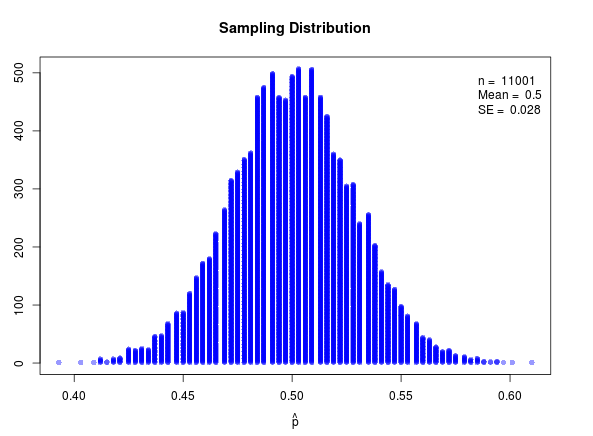
\includegraphics[width=.3\linewidth]{../plots/MIT-null.png}
\end{key}
  \item How unusual is the sample statistic from \ref{MIT.phat}
    relative to the distribution you created?  Explain in words where
    it falls relative to the plotted points.
\begin{students}
    \vspace{3cm}    
\end{students}

\begin{key}
{\it It's much bigger than any of the points I generated. The largest
  one I got was 0.585 or 186 males out of 318.}
\end{key} 
\item  How strong is the evidence against the null hypothesis?  What
  do you think about the idea that idiots are half male?
\begin{students}
    \vspace{2cm}    
\end{students}

\begin{key}
  {\it Extremely strong evidence, the p-value is less than 1 in
    1000. The null hypothesis of only half males is not 
    supported by these data. I conclude that there are more male idiots
  than female idiots.  } 
\end{key}


\end{enumerate}

\item Instead of considering a test of the true population proportion, we
  will switch gears and now estimate it.
  \begin{enumerate}
    \item What is our ``point'' estimate of the
      true proportion of idiots who are male (the sample statistic)?
\begin{students}
    \vspace{.4cm}    
\end{students}

\begin{key}
$\widehat{p} = 0.887$
\end{key}
    \item In order to generate simulated data,
      \begin{enumerate}
        \item How many individual ``idiots'' do we generate for one
          resample?
\begin{students}
    \vspace{.8cm}    
\end{students}

\begin{key} 
$318$
\end{key}
       \item Explain how you would mark 318 cards and use them to
         simulate the gender of one individual, and then another.
\begin{students}
    \vspace{2.5cm}    
\end{students}

\begin{key} 
  {\it Mark 26 ``Female'' and 282 ``Male''.  Shuffle them and draw one
  at random.  Replace the card, remix, and draw again for the second
  person.} 
\end{key}
       \item What probability of being male is used?
\begin{students}
    \vspace{.5cm}    
\end{students}

\begin{key} 
  {$0.887$}
\end{key}
       \item After resampling 318 individuals, what number do you compute?
\begin{students}
    \vspace{1.2cm}    
\end{students}

\begin{key} 
  {\it  The proportion of the 318 new draws which are male.}
\end{key}
     \end{enumerate}
     \item Use the  web applet to create  1000 or more
       resamples from the original data. 
       \begin{enumerate}
         \item Where is this distribution centered?
\begin{students}
    \vspace{.7cm}    
\end{students}

\begin{key} 
  {\it  0.887}
\end{key}
         \item What is the spread of the distribution of resampled proportions?
\begin{students}
    \vspace{.7cm}    
\end{students}

\begin{key} 
  {\it SE =  0.018}
\end{key}
         \end{enumerate}
     \item Find a 95\% confidence interval for the true proportion of
       idiots who are male.
\begin{students}
    \vspace{1.2cm}    
\end{students}

\begin{key} 
  $  (0.852, 0.925)$
\end{key}
     \item \label{longRun}Explain what the word ``confidence'' means for this
       confidence interval.
\begin{students}
    \vspace{3cm}    
\end{students}

\begin{key} 
  {\it Our confidence is in the process, not in just one interval. If
    we repeat the process (gather a new random sample) over and over,
    95\% of the intervals we create will include the true parameter of
  interest.}
\end{key}

  \end{enumerate}
\item Interpret this confidence interval.
\begin{students}
    \vspace{2cm}    
\end{students}

\begin{key} 
  {\it We are 95\% confident that the true percentage of idiots who
    are male is between 85.2\% and 92.5\%.}
\end{key}


\item Compare results from the hypothesis test and the interval
  estimate.  If the null hypothesis is true, what value should be
  included in the 95\% CI?  Explain. Do the two methods agree to some
  extent? 
\begin{students}
    \vspace{2.5cm}    
\end{students}

\begin{key} 
  {\it  If $H_0$ is true, then the interval should contain 0.50.  It
    does not, so the two inferences agree that one--half is not
    consistent with the data.} 
\end{key}
\end{enumerate}


\begin{center}
  {\bf Take Home Message:} \vspace{-.3in}
\end{center}
\begin{itemize}
  \item You just did two inferences on the same parameter.  First, we
    tested the null hypothesis that half the world's idiots are
    male.\\
      You should have reported very strong evidence against that null
      hypothesis (less than 1/1000). We can feel quite confident that
      the true proportion 
      of males in this exclusive group is more than one half.

  \item Secondly, we computed a 95\% confidence interval for the true
    proportion of idiots who are male and you interpreted the
    interval.  In \ref{longRun} you should have explained the
    long--run coverage property of the method.
  \item   There is a correspondence
    between testing and estimating.  The values inside the interval
    you found are consistent with the data, or {\bf plausible}.  Because
    0.50 is not in the interval, it is not a plausible value for this
    parameter. 
 \item 
  Questions? Make your own summary of the  lesson. 
\end{itemize}

%% Not yet using `reject the null' terminology.



\noindent
{\bf Assignment}
\begin{itemize}
%%\item D2Quiz 4 is due Feb 8.
\item Review for the exam.
\item Read  the first two pages of Unit 2 before the next class
  after the exam.  
\end{itemize}
  %% Male idiot  pgs  75 -- 77
%%  Reordering for summer 2016 renumbered 8 as 9
  \newpage

 
\def\theTopic{Unit 1 Review }
\def\dayNum{9}


\section{ Unit 1 Review }
 
  {\bf Vocabulary} Define each term:
\begin{itemize}
\item sample
\item population
\item statistic
\item parameter
\item types of variables
\item measures of center
\item measures of spread
\item sampling bias
\item $p$
\item $\phat$
 \item Null hypothesis 
 \item Alternative hypothesis
\item Strength of evidence 
\begin{key}
{\it
    The probability (proportion of simulations) of results as or
    more extreme as the observed result.}
\end{key}
\item Confidence interval\\
     Interpretation in context\\
     Meaning of ``confidence''
\item Margin of error
\item Sampling with replacement
\end{itemize}
\begin{students}
\newpage
\end{students}


\begin{center}
{\bf  Simulation}
\end{center}
\begin{enumerate}
\item If we repeat the ``Helper -- Hinderer'' study and  10 of
    the 16 infants chose the helper (6 chose hinderer):
    \begin{enumerate}
    \item How would you assess the strength of evidence using the same
      simulation we already performed?
\begin{students}
        \vspace{3.5cm}
\end{students}

\begin{key}
{\it
      Because only the observed result and nothing in the model
      actually changed, there is no reason to re-do the model.  We
      just skip to step 4 and compare the observed result to the
      null distribution. }
\end{key}
\item What strength of evidence against the null hypothesis
      does this new data provide?
\begin{students}
        \vspace{3.5cm}
\end{students}

\begin{key}
{\it
      In my simulation of 1000, there were 238 trials with 10 or
      more picking the helper, which gives a strength of evidence
      of .238 = 23.8\%}
\end{key}
\item If 13 kids chose the helper toy, what is the strength of evidence
  against the null hypothesis? 
\begin{students}
        \vspace{3.5cm}
\end{students}

\begin{key}
{\it
       With a strength of evidence of 9/1000 = .009 = .9\%, I have
      strong evidence against the null model and can conclude that
      infants do in fact use social interactions to pick a toy. }
\end{key}
\item If we redid the study with 8 infants, and 7 chose the
      helper, is this stronger, weaker, or the same amount of evidence
      against the null hypothesis?      
\begin{students}
        \vspace{3.5cm}
\end{students}
\begin{key}
{\it
      The fraction is the same, but because the sample size is
      smaller, it is less unusual to see 7 of 8 picking helper than
      to see 14 of 16.}
\end{key}
\item Explain how you would rerun the simulation for only 8 infants.
\begin{students}
        \vspace{2cm}
\end{students}
      
\begin{key}
{\it
      Change the number of trials to
      8 instead of 16.   }
\end{key}
\item Perform the simulation for 8 infants and compare the
      strength of evidence provided by 7 choosing the helper.  Was your
      hunch correct?  Explain any differences.      
\begin{students}
        \vspace{3.5cm}
\end{students}

\begin{key}
{\it
      If they said: the same, then a response might be:
      The simulation showed my answer was wrong.  There is less
      spread when the trial size was 16 than when it was 8.  Due to
      the greater spread in trial size 8, there were more trials
      with 7 or more helpers chosen (approximately 40/1000) than
      there were trials with 14 or more helpers chosen out of 16
      (approximately 1/1000). }
\end{key}
\end{enumerate}


\item A German bio-psychologist, Onur G\"{u}nt\"{u}rk\"{u}n, was
  curious whether the human tendency for right-sidedness (e.g.,
  right-handed, right-footed, right-eyed), manifested itself in other
  situations as well. In trying to understand why human brains
  function asymmetrically, with each side controlling different
  abilities, he investigated whether kissing couples were more likely
  to lean their heads to the right than to the left.  He and his
  researchers observed 124 couples (estimated ages 13 to 70 years, not
  holding any other objects like luggage that might influence their
  behavior) in public places such as airports, train stations,
  beaches, and parks in the United States, Germany, and Turkey, of
  which 80 leaned their heads to the right when kissing.
  \begin{enumerate}
    \item  What parameter is of interest?
\begin{students}
    \vspace{1.4cm}    
\end{students}
\begin{key} 
  {\it $p$ = the proportion of all couples who lean right when kissing.}
\end{key}
  \item \label{kiss.phat} What statistic do we obtain from the sample?
    Give proper notation, the statistic's value, and explain it in words.
\begin{students}
    \vspace{2cm}    \\
\end{students}
\begin{key} 
   { $\widehat{p} = \frac{80}{124} = 0.645$ \it is the
    proportion of couples leaning right.}
\end{key}
\item We can set the null hypothesis as we have before, but don't know
  before collecting data whether the alternative should be greater or
  less than one half. We therefore use a ``two-sided'' alternative
  with a $\neq$ sign.
    \begin{enumerate}
    \item State null and alternative hypotheses in symbols and
      words.\\
      $H_0:$ 
\begin{students}
    \vspace{1.5cm}    \\
\end{students}
\begin{key} 
{\it $p = .5$.  Half of all couples lean right when kissing.}
\end{key}
$H_a:$
\begin{students}
    \vspace{1cm}    \\
\end{students}
\begin{key} 
{\it $p \neq .5$.  The true proportion of couples leaning right when
  kissing is not one half.}
\end{key}
    \item How would you mark cards and randomly draw from them to
      obtain one simulated proportion drawn from the distribution when
      $H_0$ is true?
\begin{students}
    \vspace{3cm}    
\end{students}
\begin{key} 
{\it Take an even number of cards (could be 124, but a
    smaller number will also work). Mark half of them right, half
    left. Shuffle and draw one. Record the lean. Return the card
    to the deck, repeat 123 more times and divide the total number of
    right's by 124 to get one sample proportion.}
\end{key}
    \item Use the  \fbox{One Categ} -- \fbox{Test} applet to obtain
      the distribution of 1000 or more sample proportions under $H_0$.
      Sketch the picture you get here.
\begin{students}
    \vspace{5cm}    
\end{students}
\begin{key}
\ \  \\ 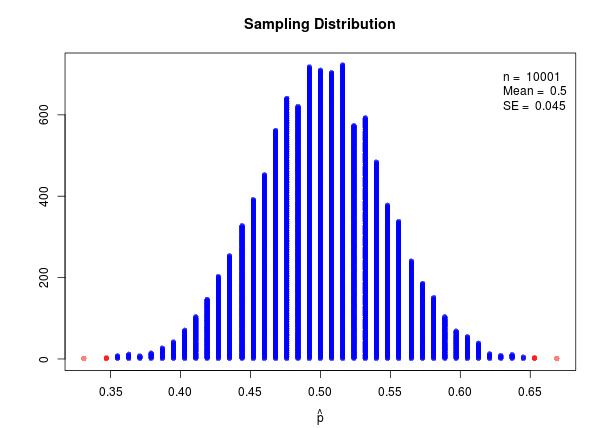
\includegraphics[width=.3\linewidth]{../plots/kissing-null.png}
\end{key}
  \item How unusual is the sample statistic from \ref{kiss.phat}
    relative to the distribution you created?  Explain in words where
    it falls relative to the plotted points.
\begin{students}
    \vspace{3cm}    
\end{students}

\begin{key}
{\it Only 8 of the 10000 points I generated are this extreme.}
\end{key} 
\item  How strong is the evidence against the null hypothesis?  What
  do you think about the idea that only half of couples lean right
  when kissing?
\begin{students}
    \vspace{2cm}    
\end{students}

\begin{key}
  {\it Extremely strong evidence, the p-value is 0.0008 which is less than 1 in
    1000. The null hypothesis of half leaning right is not consistent
    with these data. I conclude that  more than half of kissing
    couples lean to the right.  } 
\end{key}


\end{enumerate}

\item Now estimate the true population proportion.
  \begin{enumerate}
    \item What is our ``point'' estimate of the
      true proportion of couples who lean right?
\begin{students}
    \vspace{.4cm}    
\end{students}

\begin{key}
$\widehat{p} = 0.645$
\end{key}
    \item In order to generate simulated data,
      \begin{enumerate}
        \item How many couples do we generate for one resample?
\begin{students}
    \vspace{.8cm}    
\end{students}

\begin{key} 
$124$
\end{key}
       \item Explain how you would mark 124 cards and use them to
         simulate the lean of one couple, and then another.
\begin{students}
    \vspace{1.5cm}    
\end{students}

\begin{key} 
  {\it Mark 44 ``Left'' and 80 ``Right''.  Shuffle them and draw one at
    random and write down the lean on the selected card.  Replace the
    card, remix, and draw again for the second person.}
\end{key}
       \item Each couple leans right with what probability?
\begin{students}
    \vspace{.5cm}    
\end{students}

\begin{key} 
  {$0.645$}
\end{key}
       \item After resampling 124 individuals, what number would you compute?
\begin{students}
    \vspace{3.2cm}    
\end{students}

\begin{key} 
  {\it  The proportion of the 124 new draws which are right.}
\end{key}
     \end{enumerate}
     \item Use the  web applet to create  1000 or more
       resamples from the original data.
       \begin{enumerate}
         \item Where is this distribution centered?
\begin{students}
    \vspace{.7cm}    
\end{students}

\begin{key} 
  {\it  0.645}
\end{key}
         \item What number describes the spread of the distribution?
\begin{students}
    \vspace{.7cm}    
\end{students}

\begin{key} 
  {\it SE =  0.045}
\end{key}
         \end{enumerate}
%      \item   How large is the
%        margin of error for this interval?
% \begin{students}
%     \vspace{1.2cm}    
% \end{students}

% \begin{key} 
%   $ 2 * 0.045 = 0.09$
% \end{key}
     \item Compute a 99\% confidence interval.
\begin{students}
    \vspace{2.2cm}    
\end{students}

\begin{key} 
  $  (0.532, 0.742)$
\end{key}
     \item Explain what the word ``confidence'' means for this
       situation.
\begin{students}
\vspace{2cm}
\end{students}

\begin{key} 
  {\it Our confidence is in the process, not in just one interval. If
    we repeat the process (gather a new random sample) over and over,
    99\% of the intervals we create will include the true parameter of
  interest.}
\end{key}

  \end{enumerate}
\item Compare results from the hypothesis test and the interval
  estimate.  If the null hypothesis is true, what value should be
  included in the 99\% CI?  Explain. Do the two methods agree to some
  extent? 
\begin{students}
    \vspace{3.2cm}    
\end{students}

\begin{key} 
  {\it  If $H_0$ is true, then the interval should contain 0.50.  It
    does not, so the two inferences agree that one--half is not
    consistent with the data.} 
\end{key}

    \end{enumerate}
  \end{enumerate}
  

  %% Review  pgs 78 - 83
%%  Reordering for summer 2016 renumbered 9 as 10

  %% This was the ordering for Spring 2016
%   \def\theTopic{Reading 8}
 %% was 7 in Spring 2016

\section{ MIT -- the Male Idiot Theory - Reading}


The usually  serious {\em British Medical Journal} enjoys a bit
of fun in each Christmas issue.  In December 2014 they
published a study of the MIT -- ``Males are Idiots Theory'' based on
data collected from the Darwin Awards.

``Winners of the Darwin Award must die in such an idiotic
manner that `their action ensures the long-term survival of the
species, by selectively allowing one less idiot to survive.'$^{20}$ The
Darwin Awards Committee attempts to make a clear distinction
between idiotic deaths and accidental deaths. For instance,
Darwin Awards are unlikely to be awarded to individuals who
shoot themselves in the head while demonstrating that a gun is
unloaded. This occurs too often and is classed as an accident.
In contrast, candidates shooting themselves in the head to
demonstrate that a gun is loaded may be eligible for a Darwin
Award--such as the man who shot himself in the head with a
`spy pen' weapon to show his friend that it was real.$^{18}$
To qualify, nominees must improve the gene pool by eliminating
themselves from the human race using astonishingly stupid
methods. Northcutt cites a number of worthy candidates.$^{12-21}$
These include the thief attempting to purloin a steel hawser from
a lift shaft, who unbolted the hawser while standing in the lift,
which then plummeted to the ground, killing its occupant; the
man stealing a ride home by hitching a shopping trolley to the
back of a train, only to be dragged two miles to his death before
the train was able to stop; and the terrorist who posted a letter
bomb with insufficient postage stamps and who, on its return,
unthinkingly opened his own letter.''\footnote{Lendrem, B. A. D.,
  Lendrem, D. W., Gray, A., \& Isaacs, J. D. (2014). The Darwin
  Awards: sex differences in idiotic behaviour. BMJ, 349, g7094.} 

The authors examined 20 years of data on the awards, removing awards
given to couples ``usually in compromising positions'' so that each
remaining winner was either male or female. Of the 318 remaining
awards, 282 were given to males and 36 were awarded to females.

They ask the question: ``If we look only at  people who do really
stupid things, what is the gender breakdown?''  or ``Are idiots more
than half male?''

\begin{center}
  {\large\bf Questions} 
\end{center}
\begin{enumerate}
\item What population is  represented by these winners of the
     Darwin Awards?
\begin{students}
    \vspace*{5cm}    
\end{students}
\begin{key}
  {\it One could answer that winners of the award are their own small
    population, and we have a census of all Darwin Award
    winners. However, there are other idiots who have not yet won this
    competition, but seem to be working toward proving themselves. I
    would say that the sample observed represents a population of people who
    take risks which should be avoided.} 
\end{key}
\item Rephrase the researchers' question in your own words.
\begin{students}
    \vspace{2cm}    
\end{students}
\begin{key}
  {\it What proportion of really idiotic humans are male?} 
\end{key}

\item What parameter would answer that question?
\begin{students}
    \vspace{1cm}    
\end{students}
\begin{key} 
  {\it $p$ = the proportion of all idiots who are male.}
\end{key}
\item What statistic gives us information about the parameter?  What
  is its value? (Use correct notation.)
\begin{students}
    \vspace*{2cm}    \\
\end{students}
\begin{key} 
   { $\widehat{p} = \frac{282}{318} = 0.887$ \it is the
    proportion of the sample which is male.}
\end{key}

\item Would the question be better answered with a confidence interval
  or a hypothesis test? Why?
\begin{students}
    \vspace*{2cm}    \\
\end{students}
\begin{key} 
   {\it  Could go either way. CI if they focused on estimating $p$,
     or a test if they focus on ``are idiots more than half male?''.}
\end{key}

\end{enumerate}
  %% p 63-64  buff
%   \newpage

% \fancyhead[LE,RO]{
%    {\it \theTopic }\\
%    {\it Unit \unitNum\  Activity \dayNum \ Page \thepage }
% }
%  \def\theTopic{Inference on Proportions }
\def\dayNum{8}


\section{ MIT -- the Male Idiot Theory - Activity}

\begin{enumerate}
   \item  What is the parameter of interest?
\begin{students}
    \vspace{1cm}    
\end{students}
\begin{key} 
  {\it $p$ = the proportion of all idiots who are male.}
\end{key}
  \item \label{MIT.phat} What statistic do we obtain from the sample?
    Give proper notation, the statistic's value, and explain it in words.
\begin{students}
    \vspace*{2cm}    \\
\end{students}
\begin{key} 
   { $\widehat{p} = \frac{282}{318} = 0.887$ \it is the
    proportion of the sample which is male.}
\end{key}
\item Looking at the research question, ``Is the group of idiots in the world
  more than half male?'',   we set
  up the null hypothesis to assume ``just half'' and the alternative to be
  ``more than half'' male.
    \begin{enumerate}
    \item State null and alternative hypotheses in symbols and
      words.\\
      $H_0:$ 
\begin{students}
    \vspace{1.5cm}    \\
\end{students}
\begin{key} 
{\it $p = .5$.  Half of all idiots are male.}
\end{key}
$H_a:$
\begin{students}
    \vspace{1cm}    \\
\end{students}
\begin{key} 
{\it $p > .5$.  More than half of all idiots are male.}
\end{key}
    \item How would you mark cards and randomly draw from them (or use
      another random method) to
      obtain one simulated proportion drawn from the distribution when
      $H_0$ is true?
\begin{students}
    \vspace{3cm}    
\end{students}
\begin{key} 
  {\it Take an even number of cards (could be 318, but a
    smaller number will also work). Mark half of them male, half
    female. Shuffle and draw one. Record the gender. Return the card
    to the deck, repeat 317 more times and divide the total number of
    males by 318 to get one sample proportion.}
\end{key}
    \item Input the data under \fbox{One Categ} in 
      \webAppURLFrst\ 
      and then select the  \fbox{Test} page.  Do we need to change the
      ``Null value'' for $p$?\\ \ \\
      Click \fbox{1000} several times to get a distribution of sample
      proportions under $H_0$. 
      Sketch the picture you get here.
\begin{students}
    \vspace{5cm}    
\end{students}
\begin{key}
\ \  \\ 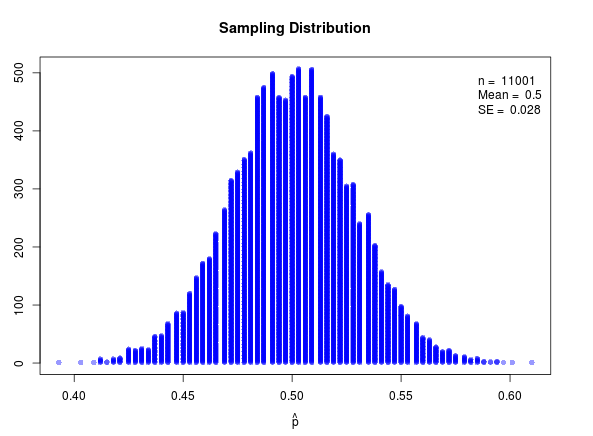
\includegraphics[width=.3\linewidth]{../plots/MIT-null.png}
\end{key}
  \item How unusual is the sample statistic from \ref{MIT.phat}
    relative to the distribution you created?  Explain in words where
    it falls relative to the plotted points.
\begin{students}
    \vspace{3cm}    
\end{students}

\begin{key}
{\it It's much bigger than any of the points I generated. The largest
  one I got was 0.585 or 186 males out of 318.}
\end{key} 
\item  How strong is the evidence against the null hypothesis?  What
  do you think about the idea that idiots are half male?
\begin{students}
    \vspace{2cm}    
\end{students}

\begin{key}
  {\it Extremely strong evidence, the p-value is less than 1 in
    1000. The null hypothesis of only half males is not 
    supported by these data. I conclude that there are more male idiots
  than female idiots.  } 
\end{key}


\end{enumerate}

\item Instead of considering a test of the true population proportion, we
  will switch gears and now estimate it.
  \begin{enumerate}
    \item What is our ``point'' estimate of the
      true proportion of idiots who are male (the sample statistic)?
\begin{students}
    \vspace{.4cm}    
\end{students}

\begin{key}
$\widehat{p} = 0.887$
\end{key}
    \item In order to generate simulated data,
      \begin{enumerate}
        \item How many individual ``idiots'' do we generate for one
          resample?
\begin{students}
    \vspace{.8cm}    
\end{students}

\begin{key} 
$318$
\end{key}
       \item Explain how you would mark 318 cards and use them to
         simulate the gender of one individual, and then another.
\begin{students}
    \vspace{2.5cm}    
\end{students}

\begin{key} 
  {\it Mark 26 ``Female'' and 282 ``Male''.  Shuffle them and draw one
  at random.  Replace the card, remix, and draw again for the second
  person.} 
\end{key}
       \item What probability of being male is used?
\begin{students}
    \vspace{.5cm}    
\end{students}

\begin{key} 
  {$0.887$}
\end{key}
       \item After resampling 318 individuals, what number do you compute?
\begin{students}
    \vspace{1.2cm}    
\end{students}

\begin{key} 
  {\it  The proportion of the 318 new draws which are male.}
\end{key}
     \end{enumerate}
     \item Use the  web applet to create  1000 or more
       resamples from the original data. 
       \begin{enumerate}
         \item Where is this distribution centered?
\begin{students}
    \vspace{.7cm}    
\end{students}

\begin{key} 
  {\it  0.887}
\end{key}
         \item What is the spread of the distribution of resampled proportions?
\begin{students}
    \vspace{.7cm}    
\end{students}

\begin{key} 
  {\it SE =  0.018}
\end{key}
         \end{enumerate}
     \item Find a 95\% confidence interval for the true proportion of
       idiots who are male.
\begin{students}
    \vspace{1.2cm}    
\end{students}

\begin{key} 
  $  (0.852, 0.925)$
\end{key}
     \item \label{longRun}Explain what the word ``confidence'' means for this
       confidence interval.
\begin{students}
    \vspace{3cm}    
\end{students}

\begin{key} 
  {\it Our confidence is in the process, not in just one interval. If
    we repeat the process (gather a new random sample) over and over,
    95\% of the intervals we create will include the true parameter of
  interest.}
\end{key}

  \end{enumerate}
\item Interpret this confidence interval.
\begin{students}
    \vspace{2cm}    
\end{students}

\begin{key} 
  {\it We are 95\% confident that the true percentage of idiots who
    are male is between 85.2\% and 92.5\%.}
\end{key}


\item Compare results from the hypothesis test and the interval
  estimate.  If the null hypothesis is true, what value should be
  included in the 95\% CI?  Explain. Do the two methods agree to some
  extent? 
\begin{students}
    \vspace{2.5cm}    
\end{students}

\begin{key} 
  {\it  If $H_0$ is true, then the interval should contain 0.50.  It
    does not, so the two inferences agree that one--half is not
    consistent with the data.} 
\end{key}
\end{enumerate}


\begin{center}
  {\bf Take Home Message:} \vspace{-.3in}
\end{center}
\begin{itemize}
  \item You just did two inferences on the same parameter.  First, we
    tested the null hypothesis that half the world's idiots are
    male.\\
      You should have reported very strong evidence against that null
      hypothesis (less than 1/1000). We can feel quite confident that
      the true proportion 
      of males in this exclusive group is more than one half.

  \item Secondly, we computed a 95\% confidence interval for the true
    proportion of idiots who are male and you interpreted the
    interval.  In \ref{longRun} you should have explained the
    long--run coverage property of the method.
  \item   There is a correspondence
    between testing and estimating.  The values inside the interval
    you found are consistent with the data, or {\bf plausible}.  Because
    0.50 is not in the interval, it is not a plausible value for this
    parameter. 
 \item 
  Questions? Make your own summary of the  lesson. 
\end{itemize}

%% Not yet using `reject the null' terminology.



\noindent
{\bf Assignment}
\begin{itemize}
%%\item D2Quiz 4 is due Feb 8.
\item Review for the exam.
\item Read  the first two pages of Unit 2 before the next class
  after the exam.  
\end{itemize}
  %% Male idiot  pgs  65 -- 67
%   \newpage
%  
\def\theTopic{Unit 1 Review }
\def\dayNum{9}


\section{ Unit 1 Review }
 
  {\bf Vocabulary} Define each term:
\begin{itemize}
\item sample
\item population
\item statistic
\item parameter
\item types of variables
\item measures of center
\item measures of spread
\item sampling bias
\item $p$
\item $\phat$
 \item Null hypothesis 
 \item Alternative hypothesis
\item Strength of evidence 
\begin{key}
{\it
    The probability (proportion of simulations) of results as or
    more extreme as the observed result.}
\end{key}
\item Confidence interval\\
     Interpretation in context\\
     Meaning of ``confidence''
\item Margin of error
\item Sampling with replacement
\end{itemize}
\begin{students}
\newpage
\end{students}


\begin{center}
{\bf  Simulation}
\end{center}
\begin{enumerate}
\item If we repeat the ``Helper -- Hinderer'' study and  10 of
    the 16 infants chose the helper (6 chose hinderer):
    \begin{enumerate}
    \item How would you assess the strength of evidence using the same
      simulation we already performed?
\begin{students}
        \vspace{3.5cm}
\end{students}

\begin{key}
{\it
      Because only the observed result and nothing in the model
      actually changed, there is no reason to re-do the model.  We
      just skip to step 4 and compare the observed result to the
      null distribution. }
\end{key}
\item What strength of evidence against the null hypothesis
      does this new data provide?
\begin{students}
        \vspace{3.5cm}
\end{students}

\begin{key}
{\it
      In my simulation of 1000, there were 238 trials with 10 or
      more picking the helper, which gives a strength of evidence
      of .238 = 23.8\%}
\end{key}
\item If 13 kids chose the helper toy, what is the strength of evidence
  against the null hypothesis? 
\begin{students}
        \vspace{3.5cm}
\end{students}

\begin{key}
{\it
       With a strength of evidence of 9/1000 = .009 = .9\%, I have
      strong evidence against the null model and can conclude that
      infants do in fact use social interactions to pick a toy. }
\end{key}
\item If we redid the study with 8 infants, and 7 chose the
      helper, is this stronger, weaker, or the same amount of evidence
      against the null hypothesis?      
\begin{students}
        \vspace{3.5cm}
\end{students}
\begin{key}
{\it
      The fraction is the same, but because the sample size is
      smaller, it is less unusual to see 7 of 8 picking helper than
      to see 14 of 16.}
\end{key}
\item Explain how you would rerun the simulation for only 8 infants.
\begin{students}
        \vspace{2cm}
\end{students}
      
\begin{key}
{\it
      Change the number of trials to
      8 instead of 16.   }
\end{key}
\item Perform the simulation for 8 infants and compare the
      strength of evidence provided by 7 choosing the helper.  Was your
      hunch correct?  Explain any differences.      
\begin{students}
        \vspace{3.5cm}
\end{students}

\begin{key}
{\it
      If they said: the same, then a response might be:
      The simulation showed my answer was wrong.  There is less
      spread when the trial size was 16 than when it was 8.  Due to
      the greater spread in trial size 8, there were more trials
      with 7 or more helpers chosen (approximately 40/1000) than
      there were trials with 14 or more helpers chosen out of 16
      (approximately 1/1000). }
\end{key}
\end{enumerate}


\item A German bio-psychologist, Onur G\"{u}nt\"{u}rk\"{u}n, was
  curious whether the human tendency for right-sidedness (e.g.,
  right-handed, right-footed, right-eyed), manifested itself in other
  situations as well. In trying to understand why human brains
  function asymmetrically, with each side controlling different
  abilities, he investigated whether kissing couples were more likely
  to lean their heads to the right than to the left.  He and his
  researchers observed 124 couples (estimated ages 13 to 70 years, not
  holding any other objects like luggage that might influence their
  behavior) in public places such as airports, train stations,
  beaches, and parks in the United States, Germany, and Turkey, of
  which 80 leaned their heads to the right when kissing.
  \begin{enumerate}
    \item  What parameter is of interest?
\begin{students}
    \vspace{1.4cm}    
\end{students}
\begin{key} 
  {\it $p$ = the proportion of all couples who lean right when kissing.}
\end{key}
  \item \label{kiss.phat} What statistic do we obtain from the sample?
    Give proper notation, the statistic's value, and explain it in words.
\begin{students}
    \vspace{2cm}    \\
\end{students}
\begin{key} 
   { $\widehat{p} = \frac{80}{124} = 0.645$ \it is the
    proportion of couples leaning right.}
\end{key}
\item We can set the null hypothesis as we have before, but don't know
  before collecting data whether the alternative should be greater or
  less than one half. We therefore use a ``two-sided'' alternative
  with a $\neq$ sign.
    \begin{enumerate}
    \item State null and alternative hypotheses in symbols and
      words.\\
      $H_0:$ 
\begin{students}
    \vspace{1.5cm}    \\
\end{students}
\begin{key} 
{\it $p = .5$.  Half of all couples lean right when kissing.}
\end{key}
$H_a:$
\begin{students}
    \vspace{1cm}    \\
\end{students}
\begin{key} 
{\it $p \neq .5$.  The true proportion of couples leaning right when
  kissing is not one half.}
\end{key}
    \item How would you mark cards and randomly draw from them to
      obtain one simulated proportion drawn from the distribution when
      $H_0$ is true?
\begin{students}
    \vspace{3cm}    
\end{students}
\begin{key} 
{\it Take an even number of cards (could be 124, but a
    smaller number will also work). Mark half of them right, half
    left. Shuffle and draw one. Record the lean. Return the card
    to the deck, repeat 123 more times and divide the total number of
    right's by 124 to get one sample proportion.}
\end{key}
    \item Use the  \fbox{One Categ} -- \fbox{Test} applet to obtain
      the distribution of 1000 or more sample proportions under $H_0$.
      Sketch the picture you get here.
\begin{students}
    \vspace{5cm}    
\end{students}
\begin{key}
\ \  \\ 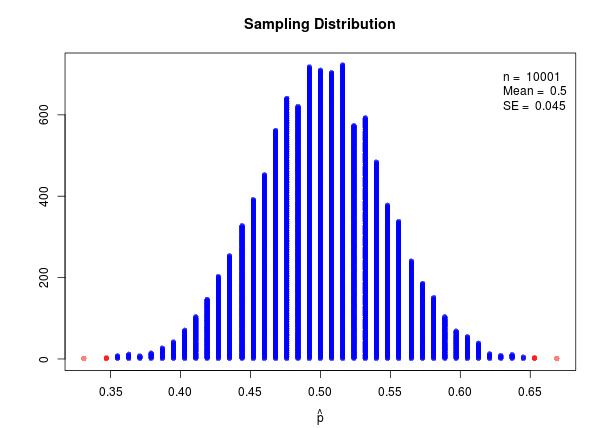
\includegraphics[width=.3\linewidth]{../plots/kissing-null.png}
\end{key}
  \item How unusual is the sample statistic from \ref{kiss.phat}
    relative to the distribution you created?  Explain in words where
    it falls relative to the plotted points.
\begin{students}
    \vspace{3cm}    
\end{students}

\begin{key}
{\it Only 8 of the 10000 points I generated are this extreme.}
\end{key} 
\item  How strong is the evidence against the null hypothesis?  What
  do you think about the idea that only half of couples lean right
  when kissing?
\begin{students}
    \vspace{2cm}    
\end{students}

\begin{key}
  {\it Extremely strong evidence, the p-value is 0.0008 which is less than 1 in
    1000. The null hypothesis of half leaning right is not consistent
    with these data. I conclude that  more than half of kissing
    couples lean to the right.  } 
\end{key}


\end{enumerate}

\item Now estimate the true population proportion.
  \begin{enumerate}
    \item What is our ``point'' estimate of the
      true proportion of couples who lean right?
\begin{students}
    \vspace{.4cm}    
\end{students}

\begin{key}
$\widehat{p} = 0.645$
\end{key}
    \item In order to generate simulated data,
      \begin{enumerate}
        \item How many couples do we generate for one resample?
\begin{students}
    \vspace{.8cm}    
\end{students}

\begin{key} 
$124$
\end{key}
       \item Explain how you would mark 124 cards and use them to
         simulate the lean of one couple, and then another.
\begin{students}
    \vspace{1.5cm}    
\end{students}

\begin{key} 
  {\it Mark 44 ``Left'' and 80 ``Right''.  Shuffle them and draw one at
    random and write down the lean on the selected card.  Replace the
    card, remix, and draw again for the second person.}
\end{key}
       \item Each couple leans right with what probability?
\begin{students}
    \vspace{.5cm}    
\end{students}

\begin{key} 
  {$0.645$}
\end{key}
       \item After resampling 124 individuals, what number would you compute?
\begin{students}
    \vspace{3.2cm}    
\end{students}

\begin{key} 
  {\it  The proportion of the 124 new draws which are right.}
\end{key}
     \end{enumerate}
     \item Use the  web applet to create  1000 or more
       resamples from the original data.
       \begin{enumerate}
         \item Where is this distribution centered?
\begin{students}
    \vspace{.7cm}    
\end{students}

\begin{key} 
  {\it  0.645}
\end{key}
         \item What number describes the spread of the distribution?
\begin{students}
    \vspace{.7cm}    
\end{students}

\begin{key} 
  {\it SE =  0.045}
\end{key}
         \end{enumerate}
%      \item   How large is the
%        margin of error for this interval?
% \begin{students}
%     \vspace{1.2cm}    
% \end{students}

% \begin{key} 
%   $ 2 * 0.045 = 0.09$
% \end{key}
     \item Compute a 99\% confidence interval.
\begin{students}
    \vspace{2.2cm}    
\end{students}

\begin{key} 
  $  (0.532, 0.742)$
\end{key}
     \item Explain what the word ``confidence'' means for this
       situation.
\begin{students}
\vspace{2cm}
\end{students}

\begin{key} 
  {\it Our confidence is in the process, not in just one interval. If
    we repeat the process (gather a new random sample) over and over,
    99\% of the intervals we create will include the true parameter of
  interest.}
\end{key}

  \end{enumerate}
\item Compare results from the hypothesis test and the interval
  estimate.  If the null hypothesis is true, what value should be
  included in the 99\% CI?  Explain. Do the two methods agree to some
  extent? 
\begin{students}
    \vspace{3.2cm}    
\end{students}

\begin{key} 
  {\it  If $H_0$ is true, then the interval should contain 0.50.  It
    does not, so the two inferences agree that one--half is not
    consistent with the data.} 
\end{key}

    \end{enumerate}
  \end{enumerate}
  

  %% Review  pgs 68 - 73

\newpage
 % \ \ \ \thispagestyle{empty}  %% p  blank white
 % \newpage

\def\unitNum{2} 
 \thispagestyle{empty}
 \vspace*{\fill}
 \begin{center}
   {\huge Unit 2}   %% p 83 - 84 blue
 \end{center}
 \vspace*{\fill}
 \newpage
 \ \ \ \thispagestyle{empty}  %% p 84 blank blue
 \newpage

\fancyhead[LE,RO]{
   {\it \theTopic }\\
   {\it Unit \unitNum\   \ Page \thepage }
}
  \def\theTopic{Reading 9}
%%  Reordering for summer 2016 renumbered 8 as 9

\section{ Experiments and Observational Studies}

\subsection{ More Types of Variables}


Sometimes a change in one variable causes another variable to change. 
For example, \vspace{-.18in}
\begin{itemize}
\item hours spent studying might affect a person's
grade in statistics
\item weight of a car might affect the gallons of fuel needed to go 100 miles
\item major in college might affect ``employment in field'' six months
  after graduation. It might also affect starting salary.
\end{itemize}
In these cases, we have an {\bf explanatory} variable which has an
effect on a  {\bf response} variable.  \\
In other cases, variables are simply {\bf associated}.  For example: \vspace{-.18in}
\begin{itemize}
\item weight and length of Rainbow trout
\item population of a city and the amount of taxes collected
\item number of beds  and  number of patient deaths per year
  in  hospitals
\item cultivated acres and annual agricultural income  in  counties
\end{itemize}
Another variable might be causing changes in both (for example the age
of the trout would affect both weight and length), or the connection might be
more complex.  Throughout this course we will be looking for
associations and trying to determine if one variable is {\bf causing}
changes in the other.  \\
{\bf Caution:} We will often find that variables are associated (or
  not), but {\bf Association does not imply causation!}   You may have
  heard people say: ``Correlation does not imply causation.''  They
  are trying to say the same thing, but in statistics, correlation has
  a very specific meaning. It is the strength (and direction) of a
  linear relationship between two quantitative variables and should
  not be used when one variable is (or both are) categorical.  For now
  just say ``association'' instead. We will get to correlation in a
  few weeks.\\
For the following scenarios, circle any explanatory variable (if there
is one) and draw an arrow to the response variable (if there is
one). % If neither affects the other, put a rectangle around each.
\begin{enumerate}
\item Textbooks:  cost, type of binding, number of pages\\
\item Chickens:  breed, diet,  weight gain\\
\item Test Scores:  Exam 1, Exam 2, Exam 3\\
\end{enumerate}


\subsection{ Types of Studies}

  Because we do often want to say that changing one variable causes
  changes in another, we need to distinguish carefully between two
  types of studies. One will allow us to conclude that there is a causal
  link;   others will not.

  {\bf Experiments} are studies in which treatments are assigned to
  the units of the study. Units (or cases) can be people -- called
  subjects -- or things like animals, plants, plots of ground.  A
  treatment variable has {\bf levels} like different drugs or dosages
  or times or oven temperatures, so it is a categorical variable. \\
  {\bf Randomized Experiments} are those in which treatments are {\bf
    randomly} assigned.  These are very special -- we'll keep an eye
  out for them.


  {\bf Observational Studies} are studies in which no variables are
  set, but each is simply observed, or measured, on the units (or
  cases). The variables could be categorical or quantitative and the
  units, as with experiments, can be subjects (people), animals,
  schools, stores, or any other entity that we can measure. 

  The next activity will discuss the differences between experiments
  and observational studies.  You'll need a bit more information about
  how experiments are set up.

 \subsection { Four Principles of Experimental Design}

  {\bf Control}.  We want the different treatments used to be as
  similar as possible.  If one group is getting a pill, then we give
  a ``control'' group a {\bf placebo} pill which is intended to have no
  physical effect.  The placebo may have a very real psychological effect 
  because often subjects who believe that they are getting a drug 
  do actually improve.  To avoid these complexities, it is also
  important that subjects be ``{\bf blind}'' to treatment -- that they
  not be told which treatment they were assigned, and, in cases where
  measurements are subjective, that the raters also not know who
  received which treatment (a double--blind study is when neither
  subject nor rater knows which treatment was assigned).  
  \\
  In an agricultural experiment which involves spraying a fertilizer
  or an herbicide, the ``control'' plots would also be sprayed, but just
  with water. 

  {\bf Randomization}.  When doctors first started applying treatments,
  they thought that they should choose which treatment was given to each
  patient. We'll soon see that such choices lead to biased results, and
  that randomization is a better strategy because it makes treatment
  and control groups most similar in the long run.  Statisticians
  recommend that we randomize whenever possible, for example, we like
  to randomize the order in which we make measurements.

  {\bf Replication}. Larger sample sizes give more accurate results,
  so we do want to make studies as large as we can afford them to
  be. Additionally, a principle of science is that  whole
  studies should be replicated.  With people, one study most often uses a
  very narrow slice of the human population, so it's a very good idea
  to run it again in a different country.  The Skeptic reading from
  page \pageref{skeptoid} mentioned ``meta analysis'' which combines results from
  multiple ESP experiments to broaden the inferences we can make about
  ESP. 

  {\bf Blocking}. Agronomists comparing yields of different wheat
  varieties (treatments), have to worry about the fact that in any
  field there are patches which are more (or less) productive than
  others. Instead of randomly assigning varieties to plots across a
  large field, they split the field into ``blocks'' which contain more
  uniform plots, and randomly assign varieties within each block. \\
  In a comparison of a new surgical technique with an old one, doctors
  might split patients into three different risk levels and assign
  treatments randomly within each group (block).  Then each treatment
  group has roughly the same number of high, medium, and low risk
  patients, and we will get a comparison of the treatments which is
  not ``confounded'' with risk level.  Studies are often blocked by
  gender or age, as well.\\
  Two variables are ``confounded'' if their effects cannot be
  separated.  For example, the first times we offered this curriculum,
  students taking a Tuesday--Thursday class all had the new curriculum
  in TEAL rooms, and the students taking MWF classes all had the old
  curriculum in non-TEAL rooms.  We saw a large improvement in average
  test scores, but could not separate the effects of ``day of week'',
  curriculum, and room type.


{\bf Important Points}:
\begin{itemize}
\item Know the difference between an explanatory variable and a
  response.\vfill
\item What is the difference between an experiment and an
  observational study?\vfill
\item How could MSU run a randomized experiment to compare two different
  types of STAT 216 curriculum?  How would we  set that up?\vfill
\item Why do clinical trials expect doctors to use a double-blind protocol?\vfill
\item What are two ways in which replication is used? \vfill
\item Suppose we want to compare two weight reduction plans.  How
  would blocking on gender change the set up of the experiment?    \vspace*{\fill}
\end{itemize}
  %% 85-88 buff 
%%  Reordering for summer 2016 renumbered 8 as 9
  \newpage


\fancyhead[LE,RO]{
   {\it Notes }\\
   {\it Unit \unitNum\   \ Page \thepage }
}
%Intentionally left blank
\phantom{No text here}
\newpage


 
\fancyhead[LE,RO]{
   {\it \theTopic }\\
   {\it Unit \unitNum\  Activity \dayNum \ Page \thepage }
}

  \def\theTopic{ Music for Studying }
\def\dayNum{11}
  %% was A10 in Sp 2016

\begin{center}
\vspace*{.1in}
{\bf {\large Does Music Help Us Study?}}\\
\end{center}
\vspace{-.1in}


Suppose you have a big test tomorrow and need to spend several hours
tonight preparing.  You'll be reviewing class notes, rereading  parts
of the textbook, going over old homework -- you know the drill.
\begin{enumerate}
\item  Which works better for you: turn on music, or study in silence? 
  Circle one:
  \begin{alist}
    \item With music
    \item In silence
  \end{alist}
  %Share answers with your group.  
  If you like to study with music (at least some times) describe:
  \begin{enumerate}
  \item what volume?\\
  \item with lyrics? or instrumental?\\
  \item what general category do you prefer?\\
  \end{enumerate}
% \item Does your group all agree?   (We doubt that.)  Do you use music
%   differently depending on the task?  Explain three or four factors
%   which influence your decision to pick a type of (or no) music.
% \begin{students}
%         \vspace{4cm}
% \end{students}
% \begin{key}
%   \\ {\it We hope that they list characteristics like
%     lyrics/instrumental, tempo, genre, mood of music.}
% \end{key}

\item A researcher wants to know if some types of music  improve or
  hurt the effectiveness of studying.  Suppose we want to address
  this question by getting college students to fill out a survey.
  \begin{enumerate}
  \item \label{response1} The survey will ask for details on the music
    type each student
    prefers for studying, but we will also need a way to measure how
    effective their studying is.  How could we measure a {\bf
      response} to use for comparison --  to see how much people are
    learning while studying?
\begin{students}
        \vspace{3cm}
\end{students}
\begin{key}
  \\ {\it This is tough. We want them to wrestle with questions of how
  much subjects knew before studying, how good a student they are, etc.
  (more in next question).  Good responses:  a post-test
  minus pre-test difference or we pick a topic which
  people don't generally know about before they study.}
\end{key}
     \item\label{lurking} In discussing the response, you probably
       found difficulties which make it hard to compare people.  What
       differences in students 
       make it hard to get a clear comparison between different music
       types?  List at least three variables that we should consider.
       For each: is it categorical or quantitative?  Focus in on
       one categorical and one quantitative variable.
\begin{students}
        \vspace{5cm}
\end{students}
\begin{key}
  \\ {\it Some students are just smarter than others (IQ is
    quantitative). The subject area of the test they are studying for (anatomy
    versus philosophy?) -- categorical. Years of musical training
    (quantitative). Surroundings (dorm room versus library) -
    categorical. Age (quantitative.) }
\end{key}
  \end{enumerate}
\item In a 2014  study of the effect of music type on studying 
  treatments were assigned.\\
   Perham, N. and Currie, H (2014). Does listening to preferred music
   improve reading comprehension performance? {\em Applied Cognitive
     Psychology} {\bf 28}:279--284.

  
   They used four levels of the variable \verb|sound|: ``disliked
   lyrical music (DLYR), liked lyrical music (LLYR), non--lyrical
   music (NLYR) and quiet (Q)'' and each subject chose music they
   liked with lyrics (LLYR), while the instrumental music (NLYR) was
   picked by the researchers, and subjects were screened to be sure they
   did not enjoy ``thrash'' music, which was used for DLYR.  Subjects
   were told to ignore the music, and had to read 70 lines of text,
   then answer four multiple choice questions about the reading (taken
   from SAT exams). They repeated the task for three more readings
   (with 4 questions each), and the proportion correct was recorded.

  \begin{enumerate}
    \item  Is use of the SAT questions an improvement over your choice
      of response in \ref{response1}?  Explain why or why not.
\begin{students}
        \vspace{4cm}
\end{students}
\begin{key}
  \\ {\it SAT will generally be better because it allows us to use a
    comparable measure across all subjects, and it is immediately
    following the music treatment.}
\end{key}
   \item   Is use of the four \verb|sound| treatments an improvement
     over asking students how they study?  Explain why or why not.
\begin{students}
        \vspace{4cm}
\end{students}
\begin{key}
  \\ {\it The four treatment levels are generally be better because
    they take away many of the options people have when choosing music.
      We can then get a direct comparison of music versus no music and
      of lyrical versus instrumental music.}
\end{key}
  
  \end{enumerate}

\item  Looking back at  the studies in 2 and 3 above, which was an experiment?
\begin{students}
        \vspace{1cm}\\
\end{students}
\begin{key}
  \\ {\it  The second one from the article by Perham and Currie.}\\
\end{key}
  Which was an observational study?  Explain how you know this.
\begin{students}
        \vspace{1cm}\\
\end{students}
\begin{key}
  \\ {\it  The survey would be observational, because music levels are
    not assigned.}
\end{key}

\end{enumerate}


\begin{center}
  {\bf Advantages of Randomized Experiments}
\end{center}

To make sure we're all thinking of the same response for our study on
the effect of music while studying, we'll focus on using the SAT
reading comprehension scores as our response.  Music (or quiet) will
be played while our subjects read and answer the questions.

\begin{enumerate}
  \setcounter{enumi}{4}
  \item In \ref{lurking}, above you mentioned several attributes of
    people which would indicate who does better on a test.  One such
    variable would be IQ.  Smarter people tend to get higher scores on
    the SAT.  
    \\ We refer to a variable like IQ as a {\bf lurking} variable when
    we do not measure it and take it into account.  What other lurking
    variables did you identify in \ref{lurking} (or add some here to
    get at least three)
    which would cause some people to do better on SAT than others?
\begin{students}
        \vspace{1cm}\\
\end{students}
\begin{key}
  \\ {\it  AWV}
\end{key}
  \item  If we don't measure IQ and don't adjust for it, we won't be
    able to tell whether one group did better because it had higher
    mean IQ, or because they were assigned the more effective treatment.  
    Let's see what happens to mean IQ (and another variable - SAT
    prep) if we randomly separate 12
    people into treatment (music) and  control (quiet) groups of 6 each.

    
\begin{tabular}{|r|c|c||r|c|c|}\hline
      \multicolumn{3}{|c||}{Treatment} &\multicolumn{3}{|c|}{Control}\\
  Name  & IQ & SAT prep & Name & IQ &SAT prep \\
\hline
Andy & 104 & Y &Peter &106 &Y\\
\hline
Ben  & 118 & Y & Maria & 90 &N\\
\hline
Betty & 79 & N & Marti & 97 &N \\
\hline
Jorge & 94 & Y & Mikaela& 98 &N\\
\hline
 Kate  & 106&N &  Patty &89 &N\\
\hline
Russ  &  88 &Y & Shawn &85 &Y\\ \hline
\end{tabular} \hfill
\begin{minipage}{.40\linewidth}
  Mean IQ of treatment group: 98.2

  Mean IQ of control group: 93.8

  Difference in means:  4.4
\end{minipage}

Write Name, IQ, and whether or not they took an SAT prep class (Yes or
No) for each person on an index card.
(If the cards are already started, check that you have the right
names and values.)  
   \begin{enumerate}
   \item Mix the cards thoroughly, and deal them into two piles of six
     each, labeling one ``T'' and the other ``C''.
     Compute the mean IQ for each group and take the difference
     ($\xb_T - \xb_C)$.\vspace{1cm}
   \item Plot your difference as instructed by your teacher. \vspace{1cm} 
\end{enumerate}

\item As with many techniques in statistics, we want to see what
  happens when we repeat the process many times.  Doing this by hand
  many times gets tedious, so we will use the computer to shuffle and
  compute means for us. \\ Go to:
  \url{https://jimrc.shinyapps.io/Sp-IntRoStats} and click
   \fbox{Lurking Demo} under \fbox{One Quant}.
   Select \fbox{IQ}. It gives you a bigger sample -- 25 IQ's in each
   group. (newly generated at random from a symmetric distribution
   with mean 100 and SD = 15).
   \begin{enumerate}
   \item Write down the means for each group in the first shuffle and
     their difference.
\begin{students}
 \vspace{1cm}
\end{students}

\begin{key}
 {\it AWV}
\end{key}

   \item Write down the means for each group in the second shuffle and
     their difference.
\begin{students}
 \vspace{1cm}
\end{students}

\begin{key}
 {\it AWV}
\end{key}
\item Compare your answers with another group's answers.  Can you
  identify a pattern?
\begin{students}
 \vspace{1cm}
\end{students}

\begin{key}
 {\it centered about zero?}
\end{key}
\end{enumerate}

\item As we said above, we need to think about repeating the shuffling
  process over and over.  Create at least  \fbox{5000} repeats and sketch the
  right-hand plot (above).  Describe the center,
  spread, and shape of this distribution.
  \begin{list}{}{}
  \item[center]
\begin{students}
 \ \  \\
\end{students}
\begin{key}
  {\it  Near 0   }
\end{key}
  \item [shape]\ 
\begin{students}
 \ \  \\
\end{students}
\begin{key}
  {\it  Symmetric  }
\end{key}
  \item [spread]\
\begin{students}
 \ \  \vspace{2cm}
\end{students}
\begin{key}
  {\it  SD $\approx 3.7$}
\end{key}
  \end{list}

\item Do we get the same pattern in the right hand plot if we run
  another batch of shuffles, say 10,000 this time?    Do
  center, shape, and/or spread change?
\begin{students}
        \vspace{2cm}\\
\end{students}
\begin{key}
  \\ {\it  No, all remain about the same.}
\end{key}


\item Note that some differences are not close to zero.  What are the
  largest and smallest values you obtained in 10,000 shuffles?
\begin{students}
        \vspace{.8cm}\\
\end{students}

\begin{key}
   {\it $\pm 12$?}
\end{key}

\item  Does randomization always make mean IQs the same
  between the two treatment groups? Explain. 
\begin{students}
 \vspace{3cm} 
\end{students}

\begin{key}
  {\it  Not  every single trial though on average (over many
    shuffles) the groups are   equivalent.  }
\end{key}
  
\item  Does randomization tend to balance out mean IQ in the long
  run, after many trials? Explain. 
\begin{students}
 \vspace{3cm} 
\end{students}

\begin{key}
  {\it  Yes, because the distribution of the difference between the two
   group means is centered at 0. }
\end{key}


  
\item {\bf Very Important Question:}  In general, how similar are
  group mean IQs when we randomly assign people into two groups?
\begin{students}
        \vspace{4cm}\\
\end{students}
\begin{key}
  \\ {\it  The difference in mean IQ between two randomized groups
    will be close to zero most of the time.  There is no guarantee for
  any one sample, but in general randomization makes the groups very
  similar.} 
\end{key}

% \item If we randomly assign levels of sound -- for simplicity, just
% LLYR or Q -- to subjects, and then find that the Q group had a much
% higher mean score on the SAT questions than the LLYR group, might 

\item Another lurking variable would be the fact that some people have
  taken a short course as an SAT prep and others haven't.  If the
  course does what it claims, then it could be the reason for one
  group to score higher than the other. We will look at the
  proportions who have taken an SAT prep course in the treatment and
  control groups.  
  \begin{enumerate}
  \item Is ``took SAT prep course'' a categorical or quantitative
    variable? 
\begin{students}
        \vspace{1cm}\\
\end{students}
\begin{key}
  \\ {\it categorical}
\end{key}

    \item Compute proportion of ``Y''s in the two groups of cards you
      had shuffled, and subtract.  Write the proportions and the
      difference here.
\begin{students}
        \vspace{1cm}\\
\end{students}
\begin{key}
  \\ {\it  AWV}
\end{key}

    \item Again go to the  web app and click \fbox{Lurking Demo}, but
      this time under \fbox{One Categ.} header.  Change {\sf A}
      to {\sf Prep} and {\sf B} to {\sf No prep} and enter the
      numbers observed in each group.  Then click \fbox{Use These
        Data}.  Run 5000 shuffles and record the mean and 
      SE of the differences $\phat_1 - \phat_2$.
\begin{students}
        \vspace{1cm}\\
\end{students}
\begin{key}
  \\ {\it AWV, but mean will be quite close to 0, SE about 0.3}
\end{key}
    \item You will have a few shuffles that give -1 or 1.  How could
      that happen? 
\begin{students}
        \vspace{1cm}\\
\end{students}
\begin{key}
  \\ {\it  One group got all the Prep people, the other group got none.}
\end{key}
 
\item The plot gets more interesting with larger counts. Suppose 
      we are randomly assigning 100 people to our two groups, and that
      28 of them have taken SAT prep, 72 have not. You can split the 28 evenly
      between Control and Treatment in the first row, and split the 72
      evenly in the bottom row. We should them have 50  Controls and
      50 in treatment. Click \fbox{Use These Data}. 
      What proportions of ``Prep'' in treatment and what differences
      do you get for the first two randomizations? 
\begin{students}
        \vspace{1cm}\\
\end{students}
\begin{key}
  \\ {\it .26, .28, differences: -0.04 and 0.00}
\end{key}
       \item Run 5000 randomizations.  Sketch your plot here.
\begin{students}
        \vspace{4cm}\\
\end{students}
\begin{key}
  
   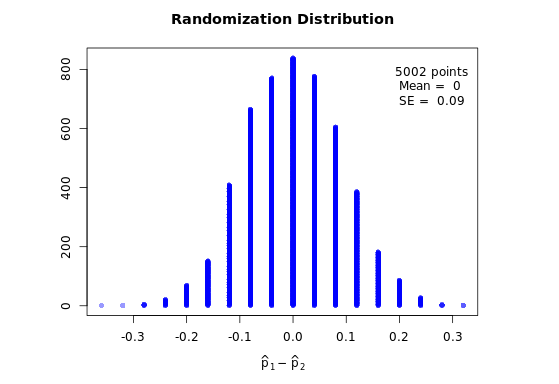
\includegraphics[width=.4\linewidth]{../plots/SATprep-shuffles.png}
\end{key}
     \item Compare with other groups.  Do the pictures look the
       same? What are its:
\begin{key}
  {\it  Yes. }
\end{key}

  \begin{list}{}{}
  \item[center?]
\begin{students}
 \ \  \\
\end{students}
\begin{key}
  {\it  Near 0 (0.00).   }
\end{key}
  \item [shape?]\ 
\begin{students}
 \ \  \\
\end{students}
\begin{key}
  {\it  Symmetric  }
\end{key}
  \item [spread?]\
\begin{students}
 \ \  \vspace{2cm}
\end{students}
\begin{key}
  {\it  around 0.09}
\end{key}
  \end{list}

\end{enumerate}

\item When we randomly assign people to two groups:
  \begin{enumerate}
  \item Is it possible for a categorical lurking variable like SAT prep
    to be imbalanced across the two groups?  Explain.
\begin{students}
    \vspace{1.5cm}\\
\end{students}
\begin{key}
  \\ {\it Yes, the proportions might differ by as much as 0.3.} 
\end{key}
  \item Will the lurking SAT variable ``usually'' be poorly balanced
    across the two groups?  Explain.
\begin{students}
        \vspace{1.5cm}\\
\end{students}
\begin{key}
  \\ {\it  No. For most of the randomizations, we get a difference in
    proportion which is close to zero, which says that about the same
    proportion of treatment people as control people have taken SAT prep. } 
\end{key}
  \end{enumerate}

\item In general, how similar is the proportion of people who have
  taken SAT prep in the treatment group to the same proportion in the
  control group? 
\begin{students}
        \vspace{3cm}\\
\end{students}
\begin{key}
  \\ {\it  The difference in proportion with SAT prep between two
    randomized groups will be close to zero most of the time.  There
    is no guarantee for any one sample, but in general randomization
    makes the groups very similar.} 
\end{key}
\item If you ran an experiment where you randomly assigned people to
  either listen to music or silence, would you have to worry about the effect
  of SAT prep courses on the results?  Explain. 
\begin{students}
        \vspace{\fill}\\
\end{students}
\begin{key}
  \\ {\it We can be pretty sure that the two randomized groups have
    similar proportions of people in them who took the SAT prep.
    Therefore, it's not a problem, and we can make out conclusions on
    the effects of music without worry about lurking variables.}
\end{key} 
\end{enumerate}


\begin{center}
  {\bf Take Home Messages}
\end{center}
  \begin{itemize}
  \item Vocabulary:  response variable, explanatory variable,
    experiment, randomized experiment, observational study, lurking
    variable.
  \item This lesson is critical for understanding how experiments
    differ from observational studies.  When we assign treatments at
    random, we ``even out'' any lurking variables, so we can say that
    differences we observe are caused by the explanatory variable (the
    treatment). We call this {\bf causal inference}.
  \item  Our use of the web app today was to see what happens to means
    of a lurking variable when we randomly split people into two
    groups. You should have concluded that the means tend to be
    approximately equal (difference in means is centered at zero), and
    that the distribution of the difference in means is symmetric. Any
    positive value has a negative counterpart which just involves
    swapping the labels (T $\longleftrightarrow$ C).

 \item 
  Any questions? 
  \end{itemize}


  
\noindent
{\bf Assignment} \vspace{-.2in}
\begin{itemize}
%\item {\bf D2Box 4} is due Feb 18. 
%    Turn it in as a pdf file in the Drop Box on D2L.
 %%  We strongly encourage you to get help in the Math Learning Center.
 % \item Watch videos \# 1 (experiments and Observational Studies) and
 %   \# 2 (Scope of Inference)  under Unit 2 before the next class. 
\item Watch videos assigned on D2L.
\item Read the next two pages before your next class.
\end{itemize}




 % means <- c(.38, .54, .37, .61)
 % sds <- c(.04, .05, .04, .05)
 % sound <- c("DLYR","noLYR","LLYR","Quiet")
 % (.61-.54)/sqrt(2*.05^2/8)
 % trt iqs
 %  t 104
 %  t 118
 %  t  79
 %  t  94
 %  t 104
 %  t  90
 %  c  97
 %  c  98
 %  c  88
 %  c 106
 %  c  89
 %  c  85
 %% Music to study by? Experiments pgs 89-96
  \newpage


\fancyhead[LE,RO]{
   {\it Notes }\\
   {\it Unit \unitNum\   \ Page \thepage }
}
%Intentionally left blank
\phantom{No text here}
\newpage


\fancyhead[LE,RO]{
   {\it \theTopic }\\
   {\it Unit \unitNum\   \ Page \thepage }
}

%%  Moved up sooner for summer
%   \def\theTopic{Reading 9}

\section{ The Sampling Distribution}


 Statistical inference is based on simple ideas of random treatment
 assignment, random selection, and random sampling.   {\bf RANDOM} 
 means that the outcome we will get cannot be known, but the
 distribution of possible outcomes can be known. 


\subsection{ Sampling Distribution for $\phat$}

 Consider selecting a random sample of 100 people with season passes
 to a local ski run and asking if they snow board more than they ski.
 Our sample will produce a sample  proportion -- a number which we
 cannot know ahead of time.  We will only select 
 one sample, and will only get to see one sample proportion, but we
 can think about the process of random selection and consider all the
 sample proportions we might have obtained.  This is a powerful way to
 think abstractly about the random selection process:
 \begin{itemize}
 \item We observe one sample.
 \item What else might we have observed?
 \end{itemize}
  The {\bf sampling distribution} is a description of all possible
  outcomes and the probabilities of obtaining each outcome.  If, for
  example, actually 48.7\%  of season pass holders board, then we
  could use a spinner to simulate the sampling distribution and would
  get a picture like this:

  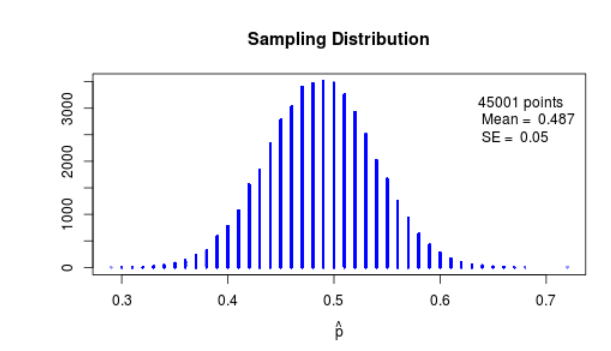
\includegraphics[width=.5\linewidth]{../plots/SampDistnofPhat-100.png}

It is centered at the true value, 0.487 as the proportion of boarders,
and has spread indicated by $SE(\phat) = 0.05$. 
%  If we decide to
% increase the sample size to 1000, the center will stay the same, but
% the spread will get smaller.
It would be very useful to know the sampling distribution so that we
could find the center part of the distribution for a confidence
interval.  

Sampling distribution for $\phat$ depends on two things: the true
parameter $p$ (unknown), and the sample size, $n$. As sample size
increases, spread gets smaller. \vspace{1in}

\subsection{ Sampling Distribution for $\xbar$}

 Now suppose we are interested in the average age of season pass
 holders in a sample of size 100. The sampling distribution  for the
 sample mean age, $\xbar$, 
 again depends on the  unknown parameter which is now $\mu$, the true
 mean age in the population,  and sample size, $n$,
 but it also depends on the spread in the original distribution,
 $\sigma$.  
 The left hand pair of plots below is for individual season pass
 holders created (not real data) under two different assumed values
 for spread, either $\sigma = 5.5$ or $\sigma = 8$.

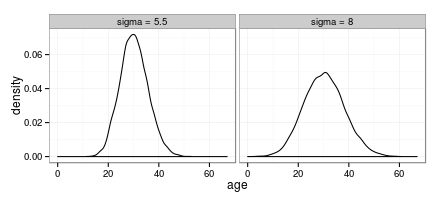
\includegraphics[width =.48\linewidth]{plots/twoSampDensities4x.png}
\hfill
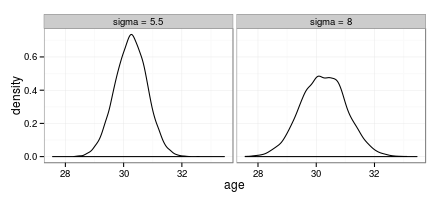
\includegraphics[width =.48\linewidth]{plots/twoSampDensities4xbar.png}\\

 The right hand pair of plots  shows the distributions of {\bf MEAN ages of 100
   season pass holders.} 

 A common confusion is to think that means will have the same
 distribution as the individuals. The two distributions will have the
 same centers, but when we average to get means, we pull in the
 extreme points.  The distribution on the right has more younger and
 older ages, but still, when averaged over 100 people (top plot) we
 rarely see a sample average as low as 28.

 Our point is that even though the distributions shown have the same
 means $\mu$, and the same $n =  100$ the different values for
 $\sigma$ change the sampling distributions for $\xbar$, the sample mean. 



 

{\bf Important Points}
\begin{itemize}
\item What does it mean to say that an outcome is ``random''?\vfill
\item Why does a plot of a sampling distribution show many points, not
  just one? After all, there is just one sample, right?\vfill
\item Sampling distributions of $\phat$ and of $\xbar$ both depend on:
  \vfill
\item Additionally, the sampling distribution for $\xbar$ depends
  on:\vfill
\item Why is the sampling distribution for $\xbar$ less spread out
  than the distribution of the original data?
\end{itemize}


%% R code
% require(ggplot2)
% sample1 <- apply(matrix(rpois(1000000,30.25), nrow=100),2,mean)
% sample2 <- apply(matrix(rpois(1000000,60.25)-30, nrow=100),2,mean)
%  sampMeanFrame <- data.frame(age = c(sample1, sample2), sample = gl(2,
%  10000, labels = c("sigma = 5.5", "sigma = 8")))
%  qplot( x = age,  facets =  ~ sample, data = sampMeanFrame, geom = "density") + theme_bw()
% dev.copy(png,file = "plots/twoSampDensities4xbar.png",height = 200,
% width = 440);dev.off()

%  sample1 <- rpois(10000,30.25)
%  sample2 <- rpois(10000,64.25)-34
%   sampXFrame <- data.frame(age = c(sample1, sample2), sample = gl(2,
%   10000, labels = c("sigma = 5.5", "sigma = 8")))
%   qplot( x = age,  facets =  ~ sample, data = sampXFrame, geom =
%   "density", adjust = 1)  + theme_bw()
%  dev.copy(png,file = "plots/twoSampDensities4x.png",height = 200, width = 440);dev.off()    %% sampling dist'n for xbar pgs 89-90 buff
%   \newpage

% \fancyhead[LE,RO]{
%    {\it \theTopic }\\
%    {\it Unit \unitNum\  Activity \dayNum \ Page \thepage }
% }
%  \def\theTopic{Textbook Costs}
\def\dayNum{8 }
 %% was 11 in Spring 2016

\section{Bootstrap  Confidence Interval for $\mu$}


We would like to know how much the ``typical'' MSU students spends on
books each semester.  Is this a question we can answer by testing?
  We need an estimate, and as you now know, we like interval
estimates because they include some information about uncertainty.

So far, the tools we have for working with a mean have allowed us to
test a pre-specified value, not estimate an unknown parameter.
We have a point estimate: a sample mean, $\xb$, but we don't know how
variable it is because we don't know $\sigma$, the true standard
deviation of the data points. 

{\bf Problem}:\\
We need to know the sampling distribution to know how far away our
statistic might be from our parameter.  We know the sampling
distribution of $ \xb$ is centered at the population mean, $\mu$, and
we know some things about its spread and shape.   However, the sampling
distribution  of $\xb$ depends on the unknown parameters $\mu$ and $\sigma$. How
can we estimate $\mu$?  


{\bf Solution}:\\Use the ``Resampling'' or Bootstrap distribution as a
substitute for the unknown sampling distribution.
\vspace{-.2in}
\begin{center}
	{\bf\sf	We only draw {\bf one} sample from the population!}
\end{center}

Hang onto that idea, because we will use our one sample  in an almost
magical way to generate something very much like the sampling
distribution.   

% When a computer ``boots up'' it goes from a dead state with no
% electrons moving through it to a live state where it's ready to accept
% instruction.  The word ``boot'' comes from ``bootstrap'' and a silly
% tale about Baron Munchausen who got himself out of quicksand by
% pulling on his bootstraps.  In statistics our objective is to take our
% one sample and create many samples from it. That seems a bit
% impossible, but computer scientists figured how to make a computer
% boot up, and similarly, statisticians have figured out how to measure
% sampling variation when we have only a single sample. 

  A {\bf bootstrap resample} is the same size as the original data, and
  consists of data points from the original data.  The only difference
  is that the resampling is done ``with replacement'' so a bootstrap
  resample typically contains several replicates of some values and is
  missing other values completely.  We can repeat this process many
  times and store the statistics generated from each resample.  The
  result is a bootstrap distribution (or a resampling distribution)
  which can be used as a replacement for the unknown sampling
  distribution.  In particular, we can use the spread (standard error)
  of the bootstrapped sample statistics as a substitute for the spread
  (standard error) of our statistic.  

   

Go to  the applet:\\
\webAppURLFrst and 
select \fbox{Bootstrap Demo}under  \fbox{One Quant}.
\vspace{-.2in}
\begin{enumerate}
  \item  The counts shown are all the values in the ``population'', which
    are amounts (in 10's of dollars) stat students in a prior semester
    spent on textbooks.  We will pretend that this is the entire
    population in order to see how well our methods work.
    \begin{enumerate}
    \item  Click \fbox{Sample} and we'll get a random sample of size
      8 from this population.  The population then disappears because
      we never can observe an entire population. Some of your numbers
      might be the same, but they came from different individuals in
      the population.  Click \fbox{Get New Sample} at the bottom of
      the page, and you'll get a new sample.  How many samples do 
       we collect in one study?
\begin{students}
        \vspace{1cm}        
\end{students}
\begin{key}
   {\it AWV. just one. }
\end{key}
    \item  Click \fbox{1 Resample} and watch what happens. Click
      \fbox{slower} 1 or 2 times and watch it again.  What is this
      button doing?
\begin{students}
        \vspace{1cm}        
\end{students}
\begin{key}
   {\it It selects 8 values from the sample with replacement, pulls
    each down to the next line, and leaves a colored spot on each one
    it grabbed.  The resample then gets combined (averaged) to a
    single value and that is plotted on the dotplot scale.}
\end{key}
    \item  Slow it down to where you can answer these questions: For
      one resample, which of the original eight values got used more
      than once? which not at all?
\begin{students}
        \vspace{1cm}        
\end{students}
\begin{key}
   {\it AWV.}
\end{key}
    \item Get 8 cards from your instructor and write each of the 8 values in
      your sample on a card.  Create your own bootstrap resample to
      mimic what the computer does.  Which of these methods works?
      (Circle one.)
      \begin{enumerate}
      \item Select one card at random, leave it out, and select
        another card.  Continue until you use all the cards.
      \item Select one card at random and write down its
        value. Replace it, reshuffle, and select another.  Continue
        until you've written down eight  values. 
      \end{enumerate}
      % Explain which technique copies what the computer does when it
      % collects one resample.
\begin{students}
        \vspace{.2cm}        
\end{students}
\begin{key}
\ \  \\
  {\it The second -- sampling With Replacement is what we are doing
    on the computer. The first way always gives the same resample
    mean -- they just change order. The second lets the resample mean vary.}
\end{key}

\item What statistic are we interested in (from the sample)?  Compute
  it for the resample. 
\begin{students}
        \vspace{1cm}        
\end{students}
\begin{key}
  \\{\it mean, $\xb$, AWV}
\end{key}

\item  Click \fbox{100}  in the ``Many Resamples'' choices.
  \begin{enumerate}
  \item  Explain  what values are being plotted.  
\begin{students}
        \vspace{2cm}        
\end{students}
\begin{key}
  \\{\it It takes  100 resamples, computes the mean of
    each, and plots the 100 resample means. }
\end{key}
  \item A common quiz/exam question is ``What does one dot
    represent?''. Explain where the values came from and what
    statistic was computed to make one dot. 
\begin{students}
        \vspace{2.5cm}        
\end{students}
\begin{key}
  \\{\it One dot is the mean of one resample which was found by
    randomly selecting 8  values from the sample with replacement. We
    then average them     together.}
\end{key}
\end{enumerate}

\item  Click \fbox{500}  in the ``Many Resamples'' choices.
 Write down the interval estimate.  Count
      (approximately) how many circles are outside the red
      lines at the left and at the right.
\begin{students}
        \vspace{1cm}        
\end{students}
\begin{key}
  \\{\it (16.4, 55.4)  I see about 12 circles below and  12 above the interval.}
\end{key}
\\
  Repeat twice more. Write down each confidence interval and guess how
  many points fall outside each.
\begin{students}
        \vspace{1cm}        
\end{students}
\begin{key}
{\it AWV. I got (18.1, 54.9), (18.3, 54.9)}
\end{key}

\item Click  1000,  5000,and 10000 in turn. Write down
  three CI's for each.  Compare the CI's.  Are some groups off-center compared
  to others?  More variable?

\begin{students}
\vspace{4cm}
\end{students}
\begin{key}
  {\it The smaller numbers of resamples give more variability in
    CI. Centers don't change.}
\end{key}


\item Go back to 500 resamples.  What happens to length of intervals
  when we change confidence levels?  Hint: choose a different
  confidence level with the buttons, then click \fbox{500} again
  to obtain the interval.\\
\begin{students}
{\large \tt
\begin{tabular}{rc}
from 95\% to 99\% --	&	intervals  \underline{\hspace*{2in}}\\
from 95\% to 90\% --	&	intervals \underline{\hspace*{2in}}\\
\end{tabular}
}
\end{students}
\begin{key}
going from 95\% to 99\%  confidence 	intervals get longer\\
going from 95\% to 90\%  confidence 	intervals get shorter
\end{key}
    \end{enumerate}


\item When we started, we saw the whole population of counts
    which has true mean  $\mu = 34.5$ (\$345).
    \begin{enumerate}
    \item  Look back at the 90\% interval you wrote down. Did it
      contain the true value? Write ``Hit'' or ``Miss''.
\begin{students}
        \vspace{1cm}        
\end{students}
\begin{key}
  {\it AWV. All of mine did.}
\end{key}

\item  We'll now pretend that we can grab new samples and we will
  build two 90\% CI's from each as a check of consistency.
 For each row of the table, click \fbox{Get New Sample} once, then
 click \fbox{1000} to get a 90\% CI for $\mu$.  Record whether your
 first interval covers 34.5 (Hits) or not (Misses). Click  \fbox{1000}
 again, and write  ``missed'' or ``hit'' in the third column.\vspace{.5cm}\\
\begin{students}
  \begin{tabular}{l|c|c|c|}
   Click \fbox{New Sample} & \fbox{1000} Hit or Missed?&  \fbox{1000}
   Hit or Missed?& Same?\\ 
    \hline
1   \ \ & \ \ & \ \ & \ \\ 
   \ \ & \ \ & \ \ & \ \\   \hline
2   \ \ & \ \ & \ \ & \ \\ 
   \ \ & \ \ & \ \ & \ \\   \hline
3   \ \ & \ \ & \ \ & \ \\ 
   \ \ & \ \ & \ \ & \ \\   \hline
4   \ \ & \ \ & \ \ & \  \\ 
   \ \ & \ \ & \ \ & \ \\   \hline
5   \ \ & \ \ & \ \ & \  \\ 
   \ \ & \ \ & \ \ & \ \\   \hline
 \end{tabular}

  \begin{tabular}{l|c|c|c|}
   Click \fbox{New Sample} & \fbox{1000} Hit or Missed?&  \fbox{1000}
   Hit or Missed?& Same?\\ 
    \hline
6   \ \ & \ \ & \ \ & \  \\ 
   \ \ & \ \ & \ \ & \ \\   \hline
7   \ \ & \ \ & \ \ & \ \\ 
   \ \ & \ \ & \ \ & \ \\   \hline
8   \ \ & \ \ & \ \ & \ \\ 
   \ \ & \ \ & \ \ & \ \\   \hline
9   \ \ & \ \ & \ \ & \  \\ 
   \ \ & \ \ & \ \ & \  \\   \hline
10   \ \ & \ \ & \ \ & \  \\ 
   \ \ & \ \ & \ \ & \  \\   \hline
  \end{tabular}
\end{students}

   In each line above put a check in the last column if the 2
   intervals agreed (both hit or both missed). 
   Does coverage depend more on the sample or on the particular resample?

\begin{students}
        \vspace{2cm}        
\end{students}
\begin{key}
 {\it The sample.  This is just like the simulation we did for
    proportions, but the method for computing the confidence interval
    is different.  We can get a ``good'' or ``bad'' sample, but given
    the sample, the method is consistent.  }
\end{key}
\end{enumerate}
\item With proportions we used $\widehat{p} \pm 2 SE$ as our
  confidence interval.  For means, we have extra variation from not
  knowing the spread, $\sigma$, so the correct multiplier depends on
  sample size as well as confidence level.  For sample size $n=8$, the
  multiplier is $t_7^* = 2.36$ for 95\% confidence, 3.50 for 99\%
  confidence, and 1.89 for 90\% confidence.  The web app shows
  standard error of the resampled means as SD, so we use this as our
  SE.  Build 90, 95, and 99\% CI's using the $\xb \pm t^* SE$ method.
  Also write the bootstrap intervals to compare.\\
  \begin{enumerate} 
  \item Compute the mean of your sample (from the 8 values, not the
    ``Mean'' printed) \\ $\xb =$ 
\begin{key} 
 {\it AWV, mine is 24.125}
\end{key}
\item a 90\% CI for $\mu$ is (show work)
\begin{students}
        \vspace{1cm}        
\end{students}
\begin{key}
 {\it AWV, $24.125 \pm  1.89 \times 5.25 = (14.2, 34.1)$\\
     Bootstrap: (15.4, 32.5)}
\end{key}
\item a 95\% CI for $\mu$ is (show work)
\begin{students}
        \vspace{1cm}        
\end{students}
\begin{key}
 {\it AWV, $24.125 \pm  2.36 \times 5.39 = (11.4, 36.8)$\\
     Bootstrap: (13.8, 35)}
\end{key}
\item a 99\% CI for $\mu$ is (show work)
\begin{students}
        \vspace{1cm}        
\end{students}
\begin{key}
 {\it AWV, $24.125 \pm  3.50 \times 5.31 = ( 5.5, 42.7)$\\
     Bootstrap: (11.3, 36.9)}
\end{key}
\end{enumerate}
\item Is there a pattern when you compare the two methods?  Are
  bootstrap percentile methods always wider? shifted? relative to the 
 $\xb \pm t^* SE$ intervals?
\begin{students}
        \vspace{3cm}        
\end{students}
\begin{key}
  \\ {\it Bootstrap intervals are narrower.  There is a tendency for
    the $\xb \pm t^* SE$ intervals to be   too symmetric. }
\end{key}

\item Challenge: based on what you've seen so far in this course what
  will happen to our interval estimates if we 
  change  sample size from 8 to  4?  From 8 to 16?\\
   Will smaller sample size shift the center?
\begin{students}
        \vspace{.5cm}        \\
\end{students}
\begin{key}
{\it No, both are unbiased.}
\end{key}

Will smaller sample size change the width?
\begin{students}
        \vspace{.5cm}        
\end{students}
\begin{key}
\\{\it Yes, width should increase.}
\end{key}

   Will larger sample size shift the center?
\begin{students}
        \vspace{.5cm}        
\end{students}
\begin{key}
\\{\it No, both are unbiased.}
\end{key}

   Will larger sample size  change the width?\\
\begin{students}
        \vspace{.5cm}        
\end{students}
\begin{key}
\\ {\it Yes, width should shrink.}
\end{key}

   Try it and record what happens to center and spread.  (Yes, it is
   important to write it down. It will show up on the exam.)  Using
   just one sample may not give you a good comparison.  Try several
   samples at each sample size. 
   \vfill
\end{enumerate}

\begin{center}
  {\bf Take Home Messages}
\end{center}
\begin{itemize}
  \item   We only get one SAMPLE, but from it we can generate many
    resamples.
  \item We can use the resampling distribution to see how much
    samples vary. It is a substitute for the unknown sampling
    distribution.
  \item Whether the interval includes the parameter or not
    depends mainly on our luck in sampling.  Most samples give statistics
    close to the parameter, but some can be farther away.
  \item We can use the bootstrap information in two ways:
    \begin{itemize}
    \item to compute the SE of the statistic
    \item to find percentiles of the resampling distribution.
    \end{itemize}
   Either method can give a confidence interval.  With symmetric data, the
   two should agree well.  These data are skewed to the right, and the
   bootstrap percentile intervals are preferred.
 \item 
  Questions?  What is not clear?\vfill
  \end{itemize}
  

\noindent
{\bf Assignment} \vspace{-.2in}
\begin{itemize}
%\item D2Box 4 is due Feb 18. 
%\item {\bf D2Quiz 5} is due Feb 22.  Fill it in online.
 %%  We strongly encourage you to get help in the Math Learning Center.
% \item View the video on Bootstrap - \# 3 under Unit 2.
\item Watch videos assigned on D2L.
 \item Fill in the top three boxes of column 2 in the Review
   Table. Skip testing and fill in the bootstrap confidence interval. 
\item Read the next two pages before your next class.
\end{itemize}

 %% book costs bootstrap mean CI   pgs 91-95  
%                                                              %% p 96 blank
%  \newpage


\fancyhead[LE,RO]{
   {\it \theTopic }\\
   {\it Unit \unitNum\   \ Page \thepage }
}
  \def\theTopic{Reading 10}

\section{ Comparative Studies}

  With the textbook cost we combined all MSU students together and did
  not try to compare parameter values across groups.  In many
  situation, however, the point of a study is to compare two or more
  groups. Here are some such example studies for you to consider. 

\begin{enumerate}
  \item  Depression is a serious problem which affects millions of
    people each year. Suppose that you are asked to 
    design a survey to compare answers of men and women to this question:\\
    {\sf If you were feeling depressed, would you visit MSU Counseling Services?}
    \begin{enumerate}
    \item How would you select male and female MSU students to
      interview?
\begin{students}
        \vfill
\end{students}
\begin{key}
 {\it AWV. They should try to get a representative sample.}
\end{key}
\item What are the variables you would collect in each interview?
      Are they categorical or quantitative? Is one explanatory? Is one a response?
\begin{students}
        \vfill
\end{students}
\begin{key}
 {\it Gender (Categorical -- possibly explanatory) and would you use
   the MSU SHS (categorical -- the response).}
\end{key}
    \item The statistical inference tools you learned in Unit 1 do not
      quite apply to this situation.  Why not? 
\begin{students}
        \vfill
\end{students}
\begin{key}
 {\it So far we've only dealt with a single proportion, and have not
   compared two groups. }
\end{key}
    \item Would this be an experiment or an observational study?
\begin{students}
        \vfill
\end{students}
\begin{key}
 {\it Observational study}
\end{key}
    \item What would be your scope of inference?
\begin{students}
        \vfill
\end{students}
\begin{key}
 {\it We will not be able to say that gender causes who would seek
   help at MSU SHS because we did not randomly assign gender.  If you
   randomly selected students from the MSU population, then we can
   extend the inference back to the population. Otherwise, it's just
   valid within the sample.}
\end{key}

    \end{enumerate}

  \item In a clinical trial 183 patients with chronic asthma were
    randomly assigned  to either placebo (n = 92) or budesonide (n = 91). After 12 weeks
    of treatment, doctors measured their lung function (Forced
    Expiration Volume in 1 second, FEV$_1$) in cc's.      
   \begin{enumerate}
    \item How do you think these patients were selected to be in the
      study? Is there a larger population they were drawn from?
\begin{students}
        \vspace*{\fill} \newpage
\end{students}
\begin{key}
 {\it They must have been referred to the study by a doctor, so they
   were not chosen at random.}
\end{key}

    \item What are the variables mentioned?
      Are they categorical or quantitative? Is one explanatory? Is one a response?
\begin{students}
        \vfill
\end{students}
\begin{key}
 {\it FEV is a quantitative response. Treatment (placebo or
   budesonide) is the categorical explanatory variable. }
\end{key}

    \item Would it be appropriate to ``block'' the patients before
      randomly assigning treatments?\begin{students}
        \vfill
\end{students}
\begin{key}
 {\it Yes, it would be good to use a pretest on FEV in order to be
   sure we have similar numbers of poor, medium, and healthy}
\end{key}

    \item What parameters would you compare between treatment and
      control groups?
\begin{students}
        \vfill
\end{students}
\begin{key}
 {\it Compare $\mu_{control}$ to $\mu_{treated}$.}
\end{key}

    \item Was this  an experiment or an observational study? 
\begin{students}
        \vfill
\end{students}
\begin{key}
 {\it a randomized experiment}
\end{key}

    \item What would be the scope of inference?
 \begin{students}
        \vfill
\end{students}
\begin{key}
 {\it We can make causal inference about the effect of the new drug on
 asthma symptoms in the sample.}
\end{key}

    \end{enumerate}
  \item Key Points:  What are two main differences between studies 1
    and 2, and how do they affect the ``Scope of inference'' for each
    study? \vfill
  \item In the last 10 years, the proportion of children who are
    allergic to peanuts has doubled in Western countries. However,
    the allergy is  not very common in some other countries where peanut
    protein is an important part of peoples' diets.   \\
     The LEAP randomized trial, reported by  Du Toit, et.al in the
     {\it  New England Journal of  Medicine} in February 2015
     identified over 500 children ages 4 to 10 months who showed some
     sensitivity to peanut protein. They randomly assigned them to two
     groups:
     \begin{itemize}
     \item Peanut avoiders: parents were told to not give their kids
       any food which contained peanuts, and
     \item Peanut eaters: parents were given a snack containing 
       peanut protein and told to feed it to their child several times
       per week (target dose was at least  6g of peanut protein per week).
     \end{itemize}
      At age 5 years, children were tested with a standard skin prick
      to see if they had an allergic reaction to peanut protein (yes
      or no).
      \begin{enumerate}
      \item What variables were measured? 
      Are they categorical or quantitative? Is one explanatory? Is one
      a response?
\begin{students}
        \vfill
\end{students}
\begin{key}
 {\it Peanut consumer or avoider (categorical, explanatory) and
   Allergic or not (categorical response).}
\end{key}

    \item Was this an experiment? was it randomized? were subjects
      blinded to the treatment?
\begin{students}
        \vspace*{\fill}
\end{students}
\begin{key}
 {\it Randomized experiment. Subject could not be blinded because of
   the diets involved.}
\end{key}

      \end{enumerate}

\end{enumerate}    %% comparative studies  pages 97-98  buff
  \newpage

\fancyhead[LE,RO]{
   {\it \theTopic }\\
   {\it Unit \unitNum\  Activity \dayNum \ Page \thepage }
}
 \def\theTopic{Peanut Allergies}
\def\dayNum{12 }

\section{ Peanut Allergies}


In the reading for today you learned about the LEAP study of peanut
allergies. 

The researchers want to answer this question:
\begin{center}
  {\large\sf  Does feeding children peanut protein prevent peanut allergies?} 
\end{center}
{\bf
Discuss the following questions	in your groups:}
\begin{enumerate}
  \item  Is there a treatment condition in this study? (If so, what?)
\begin{students}
\vspace{2cm}
\end{students}

\begin{key}
  {\it Yes, feeding an infant 6 g per week of peanut protein or avoiding
    peanut protein. }
\end{key}


  \item  What is the response variable in this study?
\begin{students}
\vspace{2cm}
\end{students}

\begin{key}
  {\it  Peanut Allergy at age 5 years. }
\end{key}

  \item  Are the variables above quantitative or categorical?
\begin{students}
\vspace{2cm}
\end{students}

\begin{key}
  {\it  Both are categorical. }
\end{key}


Results: 5 of the 245 infants getting peanut protein,  (2\%)  showed
allergic symptoms to peanuts, whereas in the peanut
avoidance group, 35 (13.7\%) of 255 infants developed allergic
symptoms to peanuts. (The two groups started with equal, somewhat
larger numbers of infants, but there were dropouts who are assumed
ignorable. )


  \item \label{PnutTable} Organize the results into a 2 by 2 table
\begin{students}

{\Large
    \begin{tabular}[c]{|l|c|c|c|} \hline
        &Peanuts (1) & Avoiders (2) & total \\ \hline
Allergic    &   &   & \\ \hline
Not Allergic&   &   & \\ \hline
Total & & & \\ \hline
    \end{tabular} 
}
\end{students}
\begin{key}

\begin{tabular}[c]{|l|c|c|c|} \hline
        &Peanuts & Avoiders & total \\ \hline
Allergic& 5  & 35  &  40\\ \hline
Not Allergic& 240  &  220 &460 \\ \hline
Total & 245  &  255 & 500\\ \hline
\end{tabular}
\end{key}

\item Of the 245 subjects assigned to the eat peanuts group, what proportion
  developed allergies? We will label this 
     $\widehat{p}_1$ because it is an estimate of $p_1$,  the true proportion
     who would become allergic if all infants ate peanut protein.  As
     in the notes for Activity 4,  we ornament $p$ with a ``hat'' on top to
     show that this is an estimate (or 
     a statistic) computed from the observed sample.  Finally, the ``1''
     subscript is to demark the first (treatment) group.
\begin{students}
\vspace{2cm}
\end{students}

\begin{key}
  {\it $\widehat{p}_1 = 5/245 = 0.02$ }
\end{key}



   \item  Of the 255 subjects assigned to the control condition, what
     proportion developed allergies? We'll call this $\widehat{p}_2$, using a ``2''
     for the control group. 
\begin{students}
\vspace{2cm}
\end{students}

\begin{key}
  {\it  $\widehat{p}_2 = 35/255 = 0.137$}
\end{key}



   \item Find the difference between the proportion of subjects
     assigned to the ``eat peanuts'' condition that became allergic and the
     proportion of subjects assigned to the control condition that
     became allergic.  $\widehat{p}_1 - \widehat{p}_2$ = 
\begin{students}
\vspace{2cm}
\end{students}

\begin{key}
  {\it  $0.02 - 0.137 = -0.117$}
\end{key}

   \item What proportion of all 500 subjects developed allergies?  This is called
     a marginal proportion because it just uses totals (the margins of
     the table, not the numbers in the middle of the table).  If the
     treatment has no effect, then this will be a good estimate of the
     true overall probability that any infant will develop peanut
     allergy, so label it $\widehat{p}_T$ where $T$ goes with ``Total''.
\begin{students}
\vspace{2cm}
\end{students}

\begin{key}
  {\it $\widehat{p}_T = 40/500 = 0.08$ }
\end{key}


   \item  Write a few sentences summarizing the results in the
     sample. This summary should include a summary of what the data
     suggest about: (1) the overall risk of becoming allergic to
     peanuts in these  subjects; (2) the differences between the two
     treatment groups; 
     and (3) whether or not the data appear to support the claim that
     peanut eating is effective. 
\begin{students}
\vspace{4cm}
\end{students}

\begin{key}
  {\it       The data suggests that overall approximately 8\% of
     participants developed peanut allergies, but the difference
     between the proportions who became allergic in the two treatment
     groups  was -11.7\%.  This appears to be a large difference which
     supports the idea that eating peanuts early helps infants avoid
     peanut allergies.}
\end{key}

   \end{enumerate}
   
   In statistics, we use data from a sample to generalize back to a
   population.  Here are some {\bf critical questions}:
   \begin{itemize}
   \item Does the higher allergy rate in the control group provide
     convincing evidence that the peanut eating is effective?
   \item Is it possible that there is no difference between the two
     treatments and that the difference observed could have arisen
     just from the random nature of putting the 500 subjects into
     groups (i.e., the luck of the draw)?
   \item Is it reasonable to believe the random assignment alone could
     have led to this large of a difference?
   \item Just by chance did they happen to assign
     more of the subjects who were going to developed allergies into the peanut
     treatment group than the control group?
   \end{itemize}
 
   To examine these questions, think about what you would generally see if 
   40 of the 500 kids were going to develop the allergy (the number of
   infants  who did in our sample) regardless of whether they ate
   peanuts or not. Under that assumption (the null), you would expect, on
   average, about 20 of those subjects to end up in each group. 

   \begin{center}
     Next we will {\bf Write out the hypotheses}
   \end{center}
  Reminder: hypotheses are always about parameters. Never use a ``hat''
   on the $p$'s in the hypothesis.  As before, the direction of the
   alternative depends on what the research is intended to show: no
   difference (could go either way, so use $\neq$), less than, or
   greater than.  You must specify which proportion is being
   subtracted from the other, because it will change the direction of
   the alternative.
 
 \begin{enumerate}
  \setcounter{enumi}{9}
   \item  The null hypothesis is: $H_0:\  p_1 = p_2$  or $H_0:\  p_1 -
     p_2 = 0$ or $p_{treat} =   p_{control}$. Is the researcher's question looking
     for an increase, decrease, or change in either direction?  Fill
     in the blank with $<$, $>$, or $\neq$ for the alternative
     hypothesis:  

\begin{students}
     $H_A:  p_{treat}$  \underline{\hspace{2cm}}   $p_{control}$
\end{students}
\begin{key}
   $H_A:  p_{treat} < p_{control}$
\end{key}     
\end{enumerate}

   We will use a {\bf permutation} test to compute our strength of
   evidence. ``Permutation''  just means that we are mixing up, or
   permuting, the group assignments.  In physical terms, it's
   shuffling the cards (40 ``allergy'' cards and 460 ``no allergy''
   cards)  and redealing them into two groups (treatment and control).
   Because  this is a randomized experiment, it's also fine to call this a
   ``randomization'' test.  We are looking at what might have happened
   if treatments were equally effective, and we reassigned individuals
   to (possibly different) groups.
 \begin{enumerate}
  \setcounter{enumi}{10}
   \item Go to the  web page:   \webAppURLFrst\ 
   and select \fbox{Enter Data} under  \fbox{\sf Two Categ}.
   Enter the numbers and labels from the table in \ref{PnutTable}.
   The proportions should agree with those above, but let's check:
   \begin{enumerate}
   \item 
     The proportion of infants in Peanut group who became allergic: \\ 
\begin{key}
 0.02       
\end{key}
   \item The proportion of infants in Control group who became allergic: \\ 
\begin{key}
 0.137       
\end{key}
\item The difference in proportions between the two groups: 
\begin{students}
\vspace{1cm}
\end{students}

\begin{key}
  {\it $ \pm 0.117$ }
\end{key}
\end{enumerate}

   \item  Click \fbox{Test} under \fbox{Two Categ},  generate  1000
     shuffles and sketch the plot below. 
\begin{students}
\vspace{4cm}
\end{students}

\begin{key}
  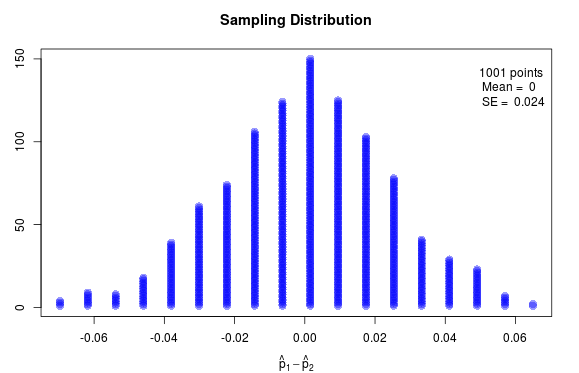
\includegraphics[width=.6\linewidth]{../plots/peanutTest-1000.png}
\end{key}

   \item  Where is the plot of the results centered (at which value)?
     Explain why this makes sense. 
\begin{students}
\vspace{2cm}
\end{students}

\begin{key}
  {\it       It is centered at 0 because 
     the null hypothesis is that the treatment has no effect on
     allergy development in which case we should see the same proportion of
     allergic kids in both groups (or the difference in
     proportions should be 0). We are assuming $H_0$ is true. }
\end{key}

   \item  
     Report the approximate p--value (i.e., strength of evidence) based
     on the observed result. (Reminder: we did this in the helper --
     hinderer study on Activity 6.)
\begin{students}
\vspace{1cm}
\end{students}

\begin{key}
  {\it  I got $0/10000 < 0.0001$}
\end{key}

       Go back to \fbox{Enter Data} and click \fbox{Use Data} to clear
       the plot. Generate another 5000 random shuffles. How  much does
       the strength of evidence change?
\begin{students}
 \vspace{1cm}
\end{students}

\begin{key}
  {\it I got $63/5000 =0.0126$. Little to no change. }
\end{key}
\vspace{1cm} 


    \item  Based on the p--value, how strong would you consider the
      evidence against the null model?  
\begin{students}
\vspace{1cm}
\end{students}

\begin{key}
  {\it    strong}
\end{key}


 
    \item  Based on the p--value, provide an answer to the research
      question.  
\begin{students}
\vspace{2cm}
\end{students}
\begin{key}
  {\it        With a p--value of 0.001, there is very  strong evidence to
      reject the null hypothesis.  We can conclude that in the
     group of infants from which these were drawn, eating peanut
     protein as an infant caused a reduction in prevalence of peanut
     allergy as evidenced by a lower proportion
      of allergic kids in the treatment group over the
      control group. }
\end{key}

    \item   Another study on the effects of a different therapy had a
      p--value of 0.25.  How would you report those results? 
\begin{students}
\vspace{3cm}
\end{students}

\begin{key}
  {\it       With a p--value of 0.25, there is little to no evidence
      against the null hypothesis.  We cannot conclude that
     the treatment prevents allergic reactions.  }
\end{key}



    \item  A third study computed p--value to be 0.73. How would you
      report those results?   
\begin{students}
\vspace*{3cm}
\end{students}

\begin{key}
  {\it        With a p--value of 0.73, there is  no evidence
      against the null hypothesis.  We cannot conclude that
      the treatment is therapeutic for patients. }
\end{key}


    \item \label{reportBullets} Write up  the pertinent
      results from the analysis. When reporting the
      results of a permutation test the following must be included:
      \begin{itemize}
      \item The type of test used in the analysis (including the
        number of trials [shuffles]);\vspace{2cm}
      \item The null model assumed in the test;\vspace{2cm}
      \item The observed result based on the data;\vspace{2cm}
      \item The p--value and strength of evidence of the test and your
        conclusion; and\vspace{2cm}
      \item The appropriate scope of inference based on the p--value
        and the study design.  Include:
        \begin{itemize}
        \item How were the subjects selected?  If they are a random
          sample from some population, then our inference goes back to
          the population.\vspace{2cm}
        \item Were treatments assigned?  If treatments were assigned
          at random, then we can state a causal conclusion.\vspace{2cm}
        \end{itemize}
      \end{itemize}
\begin{key}
 {\it      A randomization test for a difference in proportions with
      5000 trials was used to test the null hypothesis that eating
      peanut protein has no effect on whether or not an infant will
      develop peanut allergy.  In 500 participants randomly split 
      into 245 treated and 255 control babies, 40 developed peanut
      allergies: 5 in the treatment group and 35  in the control
      group.  This gave an observed difference in
      proportion of allergic kids between the treatment and
      control group of -0.117 (peanut proportion minus control).  This
      resulted in a p--value of $< 0.0001$, which constitutes  strong
      evidence against the null hypothesis.  Since participants
      were randomly assigned to groups and are representative 
      of all infants in the UK, we can
      conclude that in all UK babies, attainment's caused a lower
      proportion of infants to develop a peanut allergy as compared to a
      control group.   
     }  
\end{key}

\end{enumerate}


\begin{center}
  {\bf Take Home Messages}
\end{center}
  \begin{itemize}
  \item We are conducting a permutation test which simply mixes up the
    labels.  Because of random treatment assignment, this is also a
    randomization test. 
  \item We tested to see if  two proportions were
    equal. This is much like what we did in Unit 1 with a single
    proportion, except that the null hypothesis states that the two
    population proportions are equal (instead of one proportion coming
    from ``blind guessing'').
  \item Question \ref{reportBullets} asks you to write up results.
    Communicating 
    and reading statistical results is a very important skill.  We
    will keep doing this though the rest of the semester.  We hope you
    can dive right into the task, but if you have any questions,
    please ask.  You need to get this skill down -- the sooner the
    better. 
 \item 
 Any questions?\vfill
  \end{itemize}





\noindent
{\bf Assignment} \vspace{-.2in}
\begin{itemize}
 \item D2Box 5 is due Oct 3.
 \item {\bf D2Quiz 5} is due Oct 6.
%     Turn it in as a pdf file in the Drop Box on D2L.
 %%  We strongly encourage you to get help in the Math Learning
 %%  Center.
  \item Watch videos assigned on D2L.
  \item Fill in the top five boxes in column 3 of the Review Table.
  \item Read the next two pages before your next class.
\end{itemize}


%% Peanut Experiment  pgs 99-104
 \newpage 

\fancyhead[LE,RO]{
   {\it Notes }\\
   {\it Unit \unitNum\   \ Page \thepage }
}
%Intentionally left blank
\phantom{No text here}
\newpage


 
\fancyhead[LE,RO]{ 
   {\it \theTopic }\\
   {\it Unit \unitNum\   \ Page \thepage } 
}
  \def\theTopic{Reading 11}


\section{ Statistical Significance}

Disclaimer:  Most statisticians prefer to just report p-value as the
``strength of evidence'' and let readers evaluate the evidence against
$H_0$ for themselves.  Furthermore, if evidence from a study could be
summarized with a confidence interval, then that is a good way to
report results, too.  However, you will see results from many studies
summarized as ``statistically significant''  or as ``not statistically
significant'', so we need to talk about the meaning of those phrases.

{\bf Statistical significance} means
\begin{enumerate}
\item that researchers decided to use a  cutoff level for their study,
  typically 0.10 or 0.05 or 0.01, and
\item the p-value for the study was smaller (stronger evidence) than
  the chosen cutoff level.
\item researchers rejected the null hypothesis at the given $\alpha$
  level. 
\end{enumerate}

{\bf Significance level}, $\alpha$ is the chosen cutoff. The three
values listed above are most commonly used, but there is no reason
(other than an ingrained habit) that we could not use other levels.\\
How does one choose a significance level?
\begin{itemize}
  \item If very strong evidence is required (lives are at stake, or
    the null hypothesis has very strong support) then a small $\alpha$
    like 0.01 would be used.
  \item If we are just exploring a new area or the null hypothesis is
    not something people believe in, then weak evidence would be all
    that is needed to reject it, and we could use $\alpha = 0.10$,
\end{itemize}
 Note that people will have different opinions on the above.  That's
 why we would rather let a reader decide how strong the evidence needs
 to be.  In reports of results, we still want you to report the
 p-value. 

 {\bf Problems with fixed $\alpha$ significance testing}
 \begin{itemize}
 \item Suppose we decide to use $\alpha = 0.01$ and the p-value is
   0.0103.  We then ``Fail to reject'' at our set $\alpha$ level.  But
   someone else might repeat the study, get very similar results, and
   a p-value of 0.0098 which is less than $\alpha$, so they reject
   $H_0$.  If we just reported the p-value and let readers look at the
   strength of evidence, we would be able to say that the studies
   pretty much agree. With fixed level testing, we make quite
   different conclusions from very similar results.  That is a disturbing {\bf
     inconsistency}.
 \item P-values are strongly related to {\bf sample size}. Whether we
   ``reject'' or ``fail to reject'' depends as much on the sample size
   as it does   on the true state of nature. \\
   For example, the LEAP study of peanut allergies in the last
   activity used sample sizes of 245 and 255 infants and we had a
   p-value $< 0.0001$.  What if they had used one tenth the sample
   size as here:\\
\begin{tabular}[c]{|l|c|c|c|} \hline
        &Peanuts & Avoiders & total \\ \hline
Allergic&      0  &   4 &  4\\ \hline
Not Allergic& 24  &  22 &46 \\ \hline
Total &       24  &  26 & 50\\ \hline
\end{tabular}\\
   The proportions are almost the same, the difference in proportions
   is  $-0.15$ but the p-value is 0.066.\\
   Lessons: The researchers were smart to use a large sample
   size. However, if there was only a little difference in the two
   groups and they used a huge sample size, they would reject $p_1 =
   p_2$ when the difference in proportions allergic is very
   small. Which leads to our third point:
 \item Obtaining ``Statistical significance'' does not tell us
   anything about ``{\bf practical importance}''.  In common usage,
   the word significance  means something like ``importance''. For
   example, we talk about ``significant events'' in history. Consider
   these examples: 
   \begin{itemize}
   \item YouTube carefully examines how people navigate their web
     site.  Suppose they test two  web page designs (assigned at random) on 
     large groups of randomly selected viewers and find that there is
     a ``significant'' difference in mean time spent on their site
     (between the two designs) of 0.56 seconds ($\alpha$ was set to
     0.05). Is that an {\bf important}  difference?
\begin{key}
       \\ {\it It might be if it convinces advertisers to invest more
         in YouTube ads}.
\end{key}
   \item  Many businesses use a call center to answer questions from
     their customers.  They have to decide how many staff to have on
     hand to answer questions during business hours.  If they have too
     few people, wait times get long, and customers hang up without
     getting to a support team member. Suppose they have
     to decide between having 6 or 8 people and they do a test to
     measure the proportion of individuals who hang up before getting
     help. With 6 people the hangup proportion is 0.34 and with 8
     people it is 0.33.  Because they gathered data on several
     thousand customers, the p-value for the test is very small,
     0.002 which is ``statistically significant'' at the $\alpha =
     0.05$ level. Is a difference of 1\% of practical importance?
\begin{key}
       \\ {\it I would think not -- that they should look for other
         ways to improve service -- but it might seem important to the company.}
\end{key}
 
   \end{itemize}\vfill
 \end{itemize}



{\bf Important Points}
\begin{itemize}
\item Remember: smaller p-values provide stronger evidence against the
  null.  When we set a {\bf significance level}, we reject $H_0$ for
  p-values {\bf smaller} than $\alpha$.
\item Still report p-values.
\item Statistical significance $\neq$ practical importance.
\item When we do use a fixed $\alpha$ significance level, we will say
  either that we ``reject $H_0$'' (because p-value  $ \leq \alpha$) or
  that we ``Fail to reject $H_0$'' (when p-value $> \alpha$). We never
  accept the null hypothesis, but we can reject it.  
\end{itemize}
  %% p 105-108  buff
  \newpage

\fancyhead[LE,RO]{
   {\it Notes }\\
   {\it Unit \unitNum\   \ Page \thepage }
}
%Intentionally left blank
\phantom{No text here}
\newpage


\fancyhead[LE,RO]{ 
   {\it \theTopic }\\
   {\it Unit \unitNum\  Activity \dayNum \ Page \thepage }
}

 \def\theTopic{Weight Awareness}
\def\dayNum{13 }

\section{ What's Wrong With Your Weight?}


A study\footnote{Chang, V. W., \& Christakis,
  N. A. (2003). Self-perception of weight appropriateness in the
  United States. American Journal of Preventive Medicine, 24(4),
  332-339.}  in the {\em American Journal of Preventative Medicine},
  2003 looked at the self perception people have of their own weight.
  The participants in the {\em National Health and Nutrition
    Examination Survey} (NHNES) of the Center for Disease Control were
  asked  if they thought themselves underweight, overweight, or about
  the right weight.  Body Mass Index was also computed based on
  physical measurements, and the self--rating was compared to their
  actual classification.  The NHNES is a survey of about 5000 people each year
  which is representative of the entire US population.  The authors
  looked at data from 1999 when people were asked for their own
  perception of their weight. Interestingly, about the same
  proportion of men were wrong as women, but the way in which they
  were wrong might have a different pattern.  This table shows a
  random subsample taken from only the
  {\bf people who were wrong} in their self-perception.

  \begin{tabular}{|l|r|r|} \hline
       & \multicolumn{2}{|c|}{Gender} \\
Self Perception &Female  & Male \\ \hline
Over Estimated  &  50&  10  \\ \hline
Under Estimated &  20  & 59  \\ \hline
Total  &  70 & 69\\ \hline
  \end{tabular}
  
  The parameter of interest is $p_1 - p_2$, the true difference in
  proportions who over-estimate their weight between women and men. 
  We want to estimate how large the difference is, but first, as a
  review (as in Peanut Allergies), we'll do a test to see if the two
  proportions are equal. 
  \vspace{-.2in}
  \begin{enumerate}

  \item  State the null and alternative hypotheses in proper notation
    and in words.\\ \ 
    $H_0$
\begin{students}
 \ \   \vspace{1cm}\\
\end{students}
\begin{key}
  {\it $p_1 = p_2$  (NO HATS!) The true proportions of people who over
    estimate their weight (versus underestimate it) is zero.}
    \\
\end{key}
    $H_a$
\begin{students}
 \ \   \vspace{1cm}\\
\end{students}
\begin{key}
  {\it $p_1 \neq p_2$  (NO HATS!) The true proportions of people who over
    estimate their weight (versus underestimate it) are not equal. 
    } \\
\end{key}
    \item \label{testWeight}
   Go to the  web apps page:
   \url{https://jimrc.shinyapps.io/Sp-IntRoStats}
   and select \fbox{ Two Categ}, \fbox{Test or Estimate}.  Type our numbers into
   their cells so that \fbox{Success} is  ``over''--estimate,  \fbox{Group 1} is
   Female and change the other labels accordingly.  
   \begin{enumerate}
     \item \label{refWeights} What proportion of women who are wrong
       about their weight overestimate  (rather than underestimate) in this
       sample?  What proportion of men?  Take the difference between the two. 
\begin{students}
 \ \   \vspace*{2cm}\\
\end{students}
\begin{key}
  {\it Females: $\widehat{p}_1 = 0.714$, Males: $\widehat{p}_2 =
    0.145$,  Difference: $\widehat{p}_1  - \widehat{p}_2 =    0.569$,
    } 
\end{key}

   \item After checking the data, select \fbox{Test}, and generate  1000
     shuffles. Describe what the  computer does for a single
     ``shuffle''. 
\begin{students}
 \ \   \vspace*{3cm}\\
\end{students}
\begin{key}
  {\it  It randomly shuffles the 60 successes and 79 failures into
    fake Female and Male categories (70 females, and 69 males).}
\end{key}
% \item What does one little
%      rectangle in the histogram represent?
% \begin{students}
%  \ \   \vspace{2cm}\\
% \end{students}
% \begin{key}
%   {\it The value plotted is the difference in proportions between
%     success proportions for the fake Women and Men it created in one
%     random shuffle.}
% \end{key}

\item Why is the plot centered where it is centered?
\begin{students}
 \ \   \vspace{2cm}\\
\end{students}
\begin{key}
  {\it  Because the shuffling assumes $H_0$ is true, and that $p_1-p_2
    = 0$}
\end{key}



   \item Enter the observed difference in proportions, select the
     correct direction for the alternative, and write down the
     p--value   and strength of evidence. 
\begin{students}
 \\   \vspace{2cm}\\
\end{students}
\begin{key}
  {\it In 10000 shuffles my largest difference was 0.30, so on the
    upper side I get less than 1 in 10000. This is a two-sided
    alternative, so we have to double the one-sided count. Still the p--value
    is less than 2 in 10000 and a difference of 0.569 is enormously strong 
  evidence against the null hypothesis.    } \\
\end{key}

   \item  Which is the more plausible explanation:
     \begin{itemize}
     \item 
     These results   occurred just by chance (We just got unlucky and
     saw something weird) or
   \item 
     Men and Women who don't know what their weight is really do
     differ in their self-perception of being over versus under weight.
\begin{students}
       \vspace{2cm}
\end{students}
\begin{key}
 \\  {\it Men tend to underestimate and women to overestimate their
     weight relative to ``ideal'' weight.}  
\end{key}
     \end{itemize}
                    %%%  The S word  %%%%%%%%%%%%

    \item%  A shorthand report of statistical results often does not
      % report p--value and strength of evidence, but instead might say
      % ``the results were statistically significant at the 0.01
      % level''.  This means that the researchers determined before
      % collecting data that they wanted very strong evidence for any
      % effect, and that they would decide to ``reject $H_0$'' if the
      % p-value was less than 0.01, and that the p-value they computed
      % did turn out to be less than 0.01.  Here's a summary of the
      % steps:
      % \begin{itemize}
      % \item Decide what significance level ($\alpha$) to use,
      %   typically 0.10, 0.05 (most common) or 0.01, before collecting
      %   data.
      % \item Collect and analyze data to get a p--value.
      % \item Reject $H_o$ if the p--value $< \alpha$.  Note: we never
      %   ``accept'' $H_0$. If p--value $>\alpha$, we say that we ``Fail
      %   to reject $H_0$''.  The testing procedure can provide evidence
      %   that $H_0$ is false, but it is not intended to show that $H_0$
      %   is true.  It's like in our justice system when a defendant is
      %   found to be ``not guilty'' rather than ``innocent''.  The jury
      %   is saying that the evidence is not strong enough to
      %   ``demonstrate beyond a reasonable doubt'' that the defendant
      %   committed the crime.
      % \item If $H_0$ is rejected, some might report ``the results were
      %   statistically significant at the $\alpha$ significance
      %   level.'' (They should specify $\alpha$, but if they don't,
      %   we'd guess they used 0.05, the most common level.)
      %   This is not as informative as reporting the p--value, but you
      %   will read this in research articles, and need to know what it
      %   means. Reports for STAT 216  must contain the actual p--value.
      % \end{itemize}
      Suppose we had set $\alpha = .01$ prior to data collection. What
      is your ``decision'' about $H_0: p_1 = p_2$?  (Either reject or
      fail to reject) 
\begin{students}
 \ \   \vspace*{1cm}\\
\end{students}
\begin{key}
      \\ {\it Reject $H_0$.}\\
\end{key}
       State your conclusion about $H_0$ in the context of this
       situation. Be as specific   as possible about the true
       proportions overestimating their weight.
\begin{students}
 \ \   \vspace*{2cm}\\
\end{students}
\begin{key}
   {\it We conclude that when people are wrong about their weight, a
     much larger proportion of women than men say they are over,
     rather than under weight.}
\end{key}
\end{enumerate}

\item Now we will estimate the difference.  You might want to look
   back at Activity 7 to review the reasons we like interval estimates
   instead of point estimates.

   To build confidence intervals for a difference in proportions, we
   use the same app and data, just pick \fbox{Estimate}.

    \begin{enumerate}
      \item    \label{phatDiff} What is the point estimate for the
       difference in population    proportions? Use proper notation.
\begin{students}
 \ \   \vspace*{1cm}\\
\end{students}
\begin{key}
   $\widehat{p}_1  - \widehat{p}_2 =    0.569$
\end{key}

\item The output shows results from 1 resample of the data.
       They have generated  70 ``Female'' responses using $\phat_1 =
       50/70$ and 69 ``Male'' responses using $\phat_2 = 10/69$. What
       is the difference in proportions (over) for this one sample?
\begin{students}
 \ \   \vspace*{1cm}\\
\end{students}
\begin{key}
   \\ {\it AWV. (0.40 to 0.74) }  
\end{key}

       \item  Unlike the {\bf test} we did above, there is no assumption
         that proportions are the same for men and women.  Instead we
         use a bootstrap resample of the data on women and another bootstrap
         resample of the data on men to get an estimate of the
         sampling distribution. 
            \\  Generate more resamples until you are sure that you
            understand how they are created. For the 70 women in one
            resample, what is the probability that each will 
            ``OverEstimate'' her weight? 
\begin{students}
 \ \   \vspace*{1cm}\\
\end{students}
\begin{key}
  {\it Women: 0.714}\\
\end{key}  
For each man being resampled? 
\begin{students}
 \ \   \vspace*{1cm}\\
\end{students}
\begin{key}
  {\it  Men: 0.145}\\
\end{key} 

         How would you  resample from the women using 70 index cards?  Explain
         what to write on each card and how to randomly draw a card
         for each woman.
\begin{students}
 \ \   \vspace*{1cm}\\
\end{students}
\begin{key}
  {\it For Women, write ``Over'' on 50 cards, ``Under'' on 20  (or 5
    and 2) for 7 cards total). 
    Shuffle, draw one and record success if it's ``Over''.  Replace
    the card, shuffle, and draw the 2nd result. Continue til you get
    70 results and count up the number of ``Overs''.}
\end{key} 

        \item When you're sure you know what it is doing, click
          \fbox{\sf 1000} several times. Note that it
          adds more rather than getting rid of the old ones.
          Record center and SE of this distribution (upper right
          corner of plot).
\begin{students}
 \ \   \vspace*{1cm}\\
\end{students}
\begin{key}
   {\it I got mean$ = 0.569, SD = 0.068$}
\end{key}

\item Obtain four confidence intervals, one for each confidence
      level and write them here.
\begin{students}
 \ \   \vspace*{1cm}\\
\end{students}
\begin{key}
  \begin{tabular}{|r|c|}
    \hline
  Level & Interval \\
  80\%& (0.483, 0.656) \\
  90\% & (0.454, 0.684) \\
  95\% &(0.427, 0.699) \\
  99\% & (0.396, 0.742)
  \end{tabular}
\end{key}

\item Also compute the approximate 95\% CI using the $\pm 2 SE$ method.
   
\begin{students}
 \ \   \vspace*{1cm}\\
\end{students}
\begin{key}
   $ 0.57 \pm 2 * 0.069) =  (0.43, 0.71) $  
\end{key}
\item Compare the two 95\% intervals you created.
\begin{students}
 \ \   \vspace*{2cm}\\
\end{students}
\begin{key}
   {\it they should be quite close to each other.}\\
\end{key}

 \item Based on the 95\% CI, is it plausible that $p_1 = p_2$?
   Explain your answer by referring to your CI.
\begin{students}
 \ \   \vspace{2cm}\\
\end{students}
\begin{key}
  {\it The 95\% CI for $p_1 - p_2$ does not contain zero, so it is not
    plausible that $p_1 = p_2$. There is strong evidence that women
    tend to overestimate their weight when they are wrong, and men
    tend to underestimate.}
\end{key}
\item Interpret the meaning of this confidence interval in the context
  of this problem.  What do we mean when we say ``confidence''? 
\begin{students}
 \ \   \vspace{2cm}\\
\end{students}
\begin{key}
 {\it  We are 95\% confident that the difference in  true proportions
   (women's proportion minus men's) of people who are not in the range
   of ``ideal'' weights, but mistakenly think they are over weight is
   in the interval  (0.43, 0.71).  Our confidence is in the process, which we
   know captures the true mean 95\% of the time.}
\end{key}
    \end{enumerate}


\item Summarize the hypothesis test results in a report as in 
   question \ref{reportBullets} of the Activity 12.  Include all five
   bulleted points. 

  Note: This study did not randomly assign gender to people, it just
  observed whether they were male or female. The proper name for the
  test in \ref{testWeight} then is ``permutation'', not
  ``randomization'', and it was not 
  an experiment.  You may assume that the samples of men and women are
  representative of populations of people who are wrong about their
  weight status relative to ideal weight.\vspace{3in}

\end{enumerate}

\begin{center}
  {\bf Take Home Messages}
\end{center}
  \begin{itemize}
  \item With observational studies we can still conduct a permutation
    test, but it is not  a randomization test.
  \item As in Activity 12, we tested to see if  two proportions were
    equal. We had very strong evidence of a difference in proportions,
    but because we don't randomly assign gender, we can only say that
    we observed an {\bf association} between gender and over/under
    estimation, not that gender causes this to happen.
  \item The new part of this assignment is the confidence interval for
    the difference in proportions. 
  % \item Just reporting ``statistical significance'' has many problems.
  %   \begin{itemize}
  %   \item Statistical significance is not the same as {\bf importance}
  %     of the results.  Results could be very important, yet the
  %     p--value might not be very small, also small p--values could be
  %     attached to unimportant results.

  %   \item Journals must filter articles so that they only publish high quality
  %     research. For years, many journals thought that small p--values
  %     were an indicator of quality, but using p--values as a filter
  %     cuts out some important results. 

  %   \item By increasing sample size, we shrink the spread of the
  %     sampling distribution which tends to make p--values
  %     smaller. It's important to have large enough sample size to
  %     get a good view of the true parameter, but a really large sample
  %     lets us ``split hairs'' and label unimportant results as
  %     ``statistically significant''.

  %   \item The choice of a significance level must depend on the amount
  %     of evidence required before we're willing to give up $H_0$.  It
  %     is not the same for all situations.  The values commonly used are
  %     just based on tradition and are not especially useful.  
  %     A study with p--value 0.051 is not really different from a study
  %     of the same question which gives a p-value of 0.049.
      
  %   \end{itemize}
  \item We have just used confidence intervals 
    to estimate the difference between two proportions.  Recall from
    Activity 7: our confidence is in the process used to create the
    interval.  When used over and over on many random samples, 95\% of
    the intervals created will cover the true parameter of interest
    (here $p_1 - p_2$) and 5\% will miss the true parameter.

  \item When testing, we assume $H_0$ is true and the distribution is
    centered at 0.  When computing a bootstrap confidence interval, we
    are centered at the statistic, or point estimate, $\widehat{p}_1 -
    \widehat{p}_2$. 
 \item 
  Questions? What do you see as the key points of the lesson? \vfill

  \end{itemize}






\noindent
{\bf Assignment} \vspace{-.2in}
\begin{itemize}
\item  D2Box 5 is due Feb 25.
\item {\bf D2Quiz 6} is due Feb 29.  Fill it in online.
 %%  We strongly encourage you to get help in the Math Learning
 %%  Center.
\item Watch video 4 under Unit 2 Examples.
\item Fill in the Simulation Confidence Interval box in column 3 of
  the Review Table. 
\item Read the next two pages before your next class.
\end{itemize}

 %%  ` Wrong weight`  pgs 109-114
 \newpage


\fancyhead[LE,RO]{
   {\it Notes }\\
   {\it Unit \unitNum\   \ Page \thepage }
}
%Intentionally left blank
\phantom{No text here}
\newpage


\fancyhead[LE,RO]{
   {\it \theTopic }\\
   {\it Unit \unitNum\   \ Page \thepage }
}
  \def\theTopic{Reading 12}

\section{Energy Drinks - Reading}

In the next activity, we will use data  from this study:\\

 Curry K, Stasio MJ.  (2009). The effects of energy drinks alone and with
 alcohol on neuropsychological functioning. {\it Human  Psychopharmacology}.
{\bf 24}(6):473-81. 

Researchers used 27 volunteer college students from a private college
in the US. All were women because the college has 3 times as many
women as men, and the researchers thought it would be too hard (take
too long)  to get enough of both sexes. They advertised for
volunteers, obtained consent to drinking beverages with alcohol and or
caffiene, and were told that the study involved measuring creativity
effects. \\
The abstract says:

\begin{quotation}
  In a double-blind, placebo-controlled design, 27
  non-caffeine-deprived female participants were randomly assigned to
  consume a caffeinated energy drink alone (RED), one containing
  alcohol (RED+A), or a non-alcoholic, non-caffeinated control
  beverage. Pre- and post-test assessments were conducted using
  alternate forms of the Repeatable Battery for the Assessment of
  Neuropsychological Status (RBANS).
\end{quotation}

RBANS comes in two forms (A and B) which have been shown to give the
same scores to people in terms of cognitive status.  One form of the
test was administered several days before the subjects were given the
treatment, and another was given 30 minutes after they had drunk the
assigned beverage.  The response we will look at is the change in
RBANS scores (post score minus pre score). Initially we'll compare
only the control and RED+A groups.

The RBANS test is called a ``battery'' because it is intended to measure
many aspects of human cognition including: Immediate memory,
Visuospatial/constructional, Language, Attention, and  Delayed
memory. The scores we will examine are combined (Total scale) across
all those dimensions.  

Two of the drinks were commercial products: RED = Green Monster
(caffienated) and RED+A = Orange Sparks (6\% alcohol and caffiene)
while the control was colored Diet 7-Up.
\newpage
Questions:
\begin{enumerate}
\item What does ``double-blind'' mean for this study? \vfill
\item What are the variables of interest? What type are they?\vfill
\item Was this an experiment or an observational study?\vfill
\item Were subjects randomly chosen from some larger population of
  people?\vfill
\item If we find strong evidence of an association between the drinks
  and the ``change in RBANS'' response, what will the scope of
  inference be?  (Clearly explain and include your reasoning.)
\end{enumerate}
\normalsize   %% pages  115-116  buff
  \newpage

\fancyhead[LE,RO]{
   {\it \theTopic }\\
   {\it Unit \unitNum\  Activity \dayNum \ Page \thepage }
}

 \def\theTopic{Energy Drinks }
\def\dayNum{14}

\section{ Energy Drinks}

From Red Bull to Monster to -- you name it -- in the last few years
we've seen a large increase in the availability of so called ``Energy
Drinks''. 

{\bf Share and discuss your responses to each of the following
  questions with your group. }
\begin{enumerate}
  \item  Why are energy drinks popular? 
\begin{students}
    \vspace{4cm}    
\end{students}

\begin{key}
  {\it  AWV}
\end{key}

  \item  What claims are made in the advertising of energy drinks?
\begin{students}
     \vspace{5cm}    
\end{students}

\begin{key}
  {\it  AWV }
\end{key}

  \item  How do energy drinks interact with alcohol?
\begin{students}
    \vspace{5cm}    
\end{students}

\begin{key}
  {\it  AWV}
\end{key}

\item An experiment tried to compare the effects of energy drinks with
  and without alcohol on human subjects.  Pharmacology is the study of
  how drugs affect the body, and ``psychopharmacology'' studies
  effects of drugs on the nervous system. An article in {\it Human
    Psychopharmacology} in 2009 reported on an experiment intended to
  tease out some of the effects and to compare an energy drink without
  alcohol to one with alcohol and to a non-energy drink.  The research
  question is:

  {\sf
    Does neuropsychological performance (as measured on the RBANS
    test) change after drinking an energy drink?  After drinking an
    energy drink with alcohol? }

   Higher RBANs scores indicate better memory skills. 

Go to the site:\\
  \webAppURLFrst\ 
  Select \fbox{Test or Estimate} under \fbox{\sf One of
    Each}. Select \fbox{PreLoaded Data} as the data entry method, and
  select \fbox{REDAvsCntrl} and \fbox{Use These Data} to load today's
  data. 
 
 % \begin{fmpage}{.3\linewidth}
 % {\footnotesize
 % \begin{verbatim}
 % treatment RBAN
 % REDA	6.84
 % REDA	-9.83
 % REDA	-0.02
 % REDA	-9.12
 % REDA	-10.07
 % REDA	-19.34
 % REDA	3.97
 % REDA	-16.37
 % REDA	-21.02
 % Control	6.33
 % Control	1.65
 % Control	-3.58
 % Control	3.3
 % Control	-6.6
 % Control	3.29
 % Control	1.8
 % Control	1.8
 % Control	2.98
 % \end{verbatim}
 % }
 % \end{fmpage}
 % \hfill
% \begin{minipage}{.6\linewidth}

   Examine the boxplots and dotplots. Describe any differences in the
   response (Change in RBANS) you see  between Red+A and Control groups. \\

   Center
\begin{students}
    \vspace{1cm}    
\end{students}

\begin{key}
  {\it Mean of RED+A is clearly  lower (-8.3), Control  (1.2)\\
  Similarly, median for RED+A is -9.8; median for Control is 1.8 }
\end{key}

   Spread  (SD and IQR)
\begin{students}
    \vspace{1cm}    
\end{students}

\begin{key}
  {\it      Control has smaller spread (SD = 3.9, IQR = 1.64)
     compared to  RED+A (SD = 10.0, IQR = 10) 
}
\end{key}


   Shape
\begin{students}
    \vspace{1cm}    
\end{students}

\begin{key}
  {\it            RED+A seems most symmetric (boxplot), Cotrol
         has some outliers.
}
\end{key}
%\end{minipage}


The researchers used a computer randomization to assign the 
subjects into the groups. We'll shuffle cards instead. 

\item Here are the data in the way the experiment was run.

  \begin{tabular}{l|rrrrrrrrrr} \hline
Control&6.33&1.65&-3.58&3.30&-6.60&3.29&1.80&1.80&2.98&\\ \hline
RED+A & 6.84&-9.83&-0.02&-9.12&-10.07&-19.34&3.97&-16.37&-21.02&\\ \hline
\end{tabular}

Use the web app to find the means of these groups and subtract to find
the difference.  (Control mean minus REDA mean.) 
\begin{students}
    \vspace{1cm}    
\end{students}

\begin{key}
  {\it   $\xb_1 = -8.33$, $\xb_2 = 1.22$ ,  $\xb_1 -\xb_2 = 9.55$ }
\end{key}


\item  
We want to test the hypothesis that the means are equal:\\
  $H_0: \mu_1 = \mu_2$  (no difference in mean 'change in RBANS score'
  between REDA and control groups.)  versus:\\
  $H_a:  \mu_1 \neq \mu_2$ \hfill Consider this important question:
  \\
{\bf \sf
If the treatments have no effect on RBANS scores, then where do the
observed differences in distributions and in means come from?
}\vspace*{.2cm} \\
   Discuss this within your group and write down your answer.
  Don't say that it has anything to do with the drink they were given
  because we are assuming the drinks are all having the same effect. 
  (Give this about 2 minutes of serious discussion, then go on.
   If you get stuck here, we  won't have time to finish the activity.)
\begin{students}
    \vspace{2cm}    
\end{students}

\begin{key}
  {\it   Random variation}
\end{key}


\item  How would you use cards to reassign these 18 women into new
  treatment and control groups, and then obtain means and a new
  difference in means?
\begin{students}
    \vspace{3cm}    
\end{students}

\begin{key}
  {\it Turn the index cards over and slide them around or shuffle by
  some other method, until you think they are thoroughly mixed up.
  Line up the shuffled cards (turned face up again) in 2 rows of 9 and
  compute the mean of each row.   The means should be similar but not
  exactly the same, so the  difference in means should be about 0.}
\end{key}


\item  Suppose the first persons' change in RBANs was going to be
  6.824 no matter which drink she was given, that the second would
  always be -9.83, and so on to the last person's score of 2.98.  If
  we re-shuffle the people and deal them into two groups of 9 again
  and label then  RED+A and Control, why do the means change? (You
  are describing a model of how the data are generated) 
\begin{students}
    \vspace{2.5cm}    
\end{students}

\begin{key}
  {\it     The scores within each group change so the means change.  The person
  from RED+A no longer has to be in RED+A, etc.  Who was in which
  treatment group is randomized. 
}
\end{key}


 \item  Go back to the applet and select \fbox{Test} under \fbox{One of Each}.
   \begin{enumerate}
   \item 
   Do the means and SD's in the summary table match what we had
   earlier?  Did they subtract in the same order as we did?
\begin{students}
    \vspace{1cm}    
\end{students}

\begin{key}
  {\it  They should! If it's reversed, swap the order in the data.}
\end{key}

    \item  What are the means for control and RED+A in the
      reshuffled version?  The difference?
\begin{students}
    \vspace{1cm}    
\end{students}

\begin{key}
  {\it  AWV, but difference should be closer to 0.}
\end{key}



 \item Explain how our shuffling the cards is like what the computer does to
   the data.
\begin{students}
    \vspace{3cm}    
\end{students}

\begin{key}
  {\it  The computer just randomized which group each score came from
   similar to shuffling the scores and replacing them into different
   groups.  }
\end{key}

 \item Click \fbox{\sf 1000}   three times.  Where is the plot
   centered?   Why is it centered there?
\begin{students}
    \vspace{1.5cm}    
\end{students}

\begin{key}
  {\it     Centered close to 0 because the null is that treatment has no
   effect (i.e. the means are the same). }
\end{key}
%\vspace{3cm}


 \item  Below the plot, keep  \fbox{\sf more extreme}  and  enter the
   {\bf observed difference in means from the original data} in the
   last box.  Click \fbox{Go}. What proportion of the samples are this
   extreme?   
\begin{students}
    \vspace{1cm}    
\end{students}

\begin{key}
  {\it 0.008 in my sample. }
\end{key}

   \end{enumerate}

 \item  There are other reasons that one person might show more change
   in RBANS than another person.  Write down at least one. (Again,
   don't get stuck here.) 
\begin{students}
    \vspace{2.2cm}    
\end{students}

\begin{key}
  {\it   Genetic differences, difference in education levels, difference
     in amount of sleep the previous night, etc. 
}
\end{key}


 \item  Lurking variables were discussed on Activity 10.  When we
   randomly assign treatments, how should the groups compare on any
   lurking variable? 
\begin{students}
    \vspace{1.5cm}    
\end{students}

\begin{key}
  {\it  The should be approximately equivalent in the long run (or on average). }
\end{key}
   
 \item  Are you willing to conclude that the differences we see
   between the two groups are caused by REDA?  Explain
   your reasoning. 
\begin{students}
    \vspace{4cm}    
\end{students}

\begin{key}
  {\it  
   Most will say probably no because of the lurking variables or
   sample size (?) but we {\bf can} since we have random assignment.
 }
\end{key}
   \item We will also estimate the difference in the true
     mean RBANS change (REDA versus control) using the web app.  Select
     the \fbox{\sf  Estimate} option under \fbox{One of Each}.
      Click \fbox{10} and mouse over the extreme dots in the plot.
       Notice how the lower boxplots, the lower summary table and the
       difference in means change.  The app is creating a  
       bootstrap resample from the 9 REDA values and a bootstrap
       resample from the 9 Control values, finding the mean of each,
       and subtracting to get a difference in means which shows up in
       the plot.  Click again until you are positive you know what it
       is doing. For your last  resample, write the two bootstrap
       means and their difference. 
\begin{students}
    \vspace{2cm}    
\end{students}

\begin{key}
  {\it  I got 1.09 for Control, -7.97 for REDA with difference = -9.06.  }
\end{key}
    \item Obtain a 95\% bootstrap percentile interval based on several
      1000 resamples and write it here.
\begin{students}
    \vspace{2cm}    
\end{students}

\begin{key}
  {\it (2.84, 16.01)  }
\end{key}
    \item Write your interpretation of this interval.
\begin{students}
    \vspace{4cm}    
\end{students}

\begin{key}
  {\it  We are 95\% confident that the true mean ``change in RBANS score''
  is  2.8 to 16.01 points lower when people drink REDA than when they
   drink the control beverage. Be sure to indicate which one is higher
 (or lower). } 
\end{key}
\item Build a 95\% confidence interval using ``estimate $\pm t^*$SE'' where the
  estimate is the observed difference in means, $t^* = 2.12$, and
  using the SE the plot.  Does it contain zero?
 \begin{students}
    \vspace{2cm}    
\end{students}

\begin{key}
  {\it (2.45, 16.65 )  No.}
\end{key}


\item Write up the results of the hypothesis test as a report using
  the five elements from Activity 12.  Be sure to refer to the response
  variable as ``change in RBANS'', not just RBANS score. \\ 

\begin{students}
 \newpage 
\end{students}

\begin{key}
  {\it 
We performed a randomization (permutation) test of 5000 simulations
from the null distribution which assumed equal means for REDA and
control groups change in RBANS scores.\\
We observed a control mean (for 9 women) which was 9.55 points higher
than the REDA mean.\\
The simulated p-value was less than 1/5000 which provides very strong
evidence against the null hypothesis, so we can reject the null (at
any commonly used $\alpha$ level and conclude that the true REDA mean
change in RBANS is lower than the true Control mean.\\
We did not start with a random sample of college women, but treatments
were randomly assigned, so we can infer that REDA causes a decrease in
mean change in RBANS scores in this sample of women.
}
\end{key}


 \end{enumerate}


{\sf\bf Take Home Messages:}
\begin{itemize}
  \item 
  If there is no treatment effect, then differences in distribution
  are just due to the random assignment of treatments.  This
  corresponds to a ``null hypothesis'' of no difference between
  treatment groups.
\item  By randomly applying treatments, we are creating groups that
  should be very similar because differences between groups (age,
  reaction to alcohol, memory) are “evened out” by the random group
  allocation. If we see a difference between groups, then we doubt the
  null hypothesis that treatments don't matter.  Any difference
  between groups is caused by the treatment applied.  Random
  assignment is a very powerful tool.  When reading a study, it's one
  of the key points to look for. 
 \item When we report results about a difference in means, we {\bf
     must} specify the direction of subtraction. 
 \item 
  Questions? Summarize  the  lesson. \vfill

\end{itemize}



\noindent
{\bf Assignment} \vspace{-.2in}
\begin{itemize}
\item D2Box 6 is due Oct 10.
\item {\bf D2Quiz 6} is due Oct 13.
%    Turn it in as a pdf file in the Drop Box on D2L.
 %%  We strongly encourage you to get help in the Math Learning
 %%  Center.
\item Watch videos assigned on D2L.
%  \item Watch videos 5 and 6 under Unit 2 Examples.
\item Fill in the top six  boxes in column 4 (one  of each type) of
  the Review Table.   
\item Read the next page before your next class.
\end{itemize}


{\sf\bf Reference}
\\
 Curry K, Stasio MJ.  (2009). The effects of energy drinks alone and with
 alcohol on neuropsychological functioning. {\it Human  Psychopharmacology}.
{\bf 24}(6):473-81. doi: 10.1002/hup.1045. 


  %% Energy Drinks 6 pgs 117-122
 \newpage

\fancyhead[LE,RO]{
   {\it Notes }\\
   {\it Unit \unitNum\   \ Page \thepage }
}
%Intentionally left blank
\phantom{No text here}
\newpage


\fancyhead[LE,RO]{
   {\it \theTopic }\\
   {\it Unit \unitNum\   \ Page \thepage }
}
  \def\theTopic{Reading 13}

\section{ Hypothesis Test for a Single Mean}

Watch the video: Hypothesis Test for a Single Mean found:\\
\url{??}

{\bf Questions}:
\begin{itemize}
  \item Why might people care about average snow depth in the
    mountains around Bozeman and whether or not it has changed
    recently?\vspace{2cm}
  \item Over the 30 years before 2011, what was average snow depth at
    Arch Falls?\vspace{2cm} %% 38 in
  \item Over the past 5 years, what has average snow depth at Arch
    Falls been? \vspace{2cm}%%34.7
  \item What variable is of interest? Is it quantitative or
    categorical? What statistic will we use to summarize it?\vspace{2cm}
  \item What are the null and alternative hypotheses?\vspace{2cm}
  \item Step 2 -- to create the null distribution -- uses a technique
    you've never seen before, and it's a bit weird. We'll work on it
    in the next class activity, so if you don't get it from the video,
    that's OK.\vspace{2cm}
  \item Aside from getting the simulated distribution, everything else
    should seem familiar. Why do we want the distribution to have the
    center it does?\vspace{2cm}
  \item How do we determine the p-value in this case? What is
    it?\vspace{2cm}  
  \item What do we conclude?\vspace*{\fill}
\end{itemize}


   %% pages 123-126  buff
  \newpage

\fancyhead[LE,RO]{
   {\it Notes }\\
   {\it Unit \unitNum\   \ Page \thepage }
}
%Intentionally left blank
\phantom{No text here}
\newpage



\fancyhead[LE,RO]{
   {\it \theTopic }\\
   {\it Unit \unitNum\  Activity \dayNum \ Page \thepage }
}

 \def\theTopic{Arsenic}
\def\dayNum{15 }

\section { Arsenic in Toenails}

 Symptoms of low--level  arsenic poisoning
include headaches, confusion, severe diarrhea and
drowsiness.  When the poisoning becomes acute, symptoms include
vomiting, blood in the urine, hair loss, convulsions, and even death.
A 2007 study by Peter Ravenscroft found that over 137 million people
in more than 70 countries are probably affected by arsenic poisoning
from drinking water.\footnote{Ravenscroft, P. (2007). The global
  dimensions of arsenic pollution of groundwater. {\em Tropical
    Agriculture Association}, {\bf 3}.}

Scientists can assay toe nail clippings to measure a person's arsenic
level in parts per million (ppm).  They did this assay on 19 randomly selected 
individuals who drink from private wells in New Hampshire (data in the
table below). They want to know  the mean arsenic 
concentration for New Hampshire residents drinking from private wells.

 An arsenic level greater than 0.150 ppm is considered
hazardous. A secondary question is, ``Is there evidence that people
drinking the ground water in New Hampshire are suffering from arsenic
poisoning?''


\begin{center}
\begin{tabular}{|r|r|r|r|r|r|r|r|r|r|} \hline
0.119& 0.118& 0.099& 0.118& 0.275& 0.358& 0.080& 0.158& 0.310& 0.105
\\ \hline
0.073& 0.832& 0.517& 0.851& 0.269& 0.433& 0.141& 0.135& 0.175 & \\ \hline
\end{tabular}  
\end{center}


{\bf Step 1. State the research question. }
\begin{enumerate}
\item  \label{researchQs}Based on the description of the study, state the two research
  questions to be answered.

\begin{key}
  {\it 
    \begin{enumerate}
    \item How high is the mean arsenic level for New Hampshire residents
 drinking from a private well?
    \item Is there evidence that people drinking the ground water in New
 Hampshire are building up a hazardous  level (over 0.15 on average)
 of arsenic concentration? 

    \end{enumerate}
}
\end{key}
  

\item  Which research question should be answered using a hypothesis
  test and which should be answered using a confidence interval? 

\begin{students}
  \vspace{1.5cm}
\end{students}

\begin{key}
  {\it The first should be answered with a CI because we are trying to
    estimate the parameter,  and the second with a test (is there evidence?)}
\end{key}
\end{enumerate}

{\bf Step 2. Design a study and collect data. }
  \begin{enumerate}
  \setcounter{enumi}{2}
   \item  What is the variable in the study?  Is this variable quantitative
     or categorical?
\begin{students}
  \vspace{2.5cm}
\end{students}

\begin{key}
  {\it Arsenic concentration in toenails (ppm), quantitative.}
\end{key}

\item 
Define the parameter of interest in the context of the study.  What
notation should be used to denote it?
\begin{students}
  \vspace{1cm}
\end{students}

\begin{key}
  {\it notation: $\mu$, is mean arsenic concentration in toenails for New Hampshire residents with a private well.}
\end{key}
\end{enumerate}

{\bf Step 3. Explore the data. }\\
With quantitative data, we typically report and study the average value, or the mean.
\begin{enumerate}
\setcounter{enumi}{4}
\item  What is the sample size in this study?  n = \begin{key}
  {\it 19}
\end{key}

\item \label{xbar} Calculate the observed statistic and use correct notation to
  denote it (check your answer with another  group!).
\begin{students}
  \vspace{1cm}
\end{students}
\begin{key}
   $ \xb =   0.272$. 
\end{key}
\item  Could your answer to \ref{xbar} have happened if the arsenic
  concentrations in New Hampshire residents are not hazardous? 
\begin{students}
  \vspace{1cm}
\end{students}
\begin{key}
   {\it Yes, pretty much anything is possible if at least a few people
     have high arsenic levels.}  
\end{key}
\item  Do you think it is likely to have observed a mean like the one
  you got in \ref{xbar} if the arsenic concentrations in New Hampshire
  residents are not hazardous?
  
\begin{students}
  \vspace{1cm}
\end{students}
\begin{key}
   {\it Not sure.  Depends on how variable arsenic concentrations are!
}
\end{key}
\end{enumerate}


{\bf Step 4. Draw inferences beyond the data. }\\
We'll start with the first research question asked because we have
done confidence intervals for a single mean back in Activity 11. 

{\bf The First Research Question}: How high is the mean arsenic level
for New Hampshire residents with a private well? 

\begin{enumerate}
 \setcounter{enumi}{8}
\item  Explain why this question is better answered using a confidence
  interval than by conducting a hypothesis test. 
\begin{students}
  \vspace{1cm}
\end{students}
\begin{key}
  {\it  Because we want to estimate the parameter (how high?), not
    compare it to some value.}
\end{key}

\item  Explain how you can use a deck of 19 cards to create the
  bootstrap distribution. (Go back to Activity 11 if you don't remember.)
\begin{students}
  \vspace{1cm}
\end{students}
\begin{key}
  {\it Write the original data on the cards, then sample with replacement 19
    times.}
\end{key}

\item Use the \fbox{One Quant} option in the web applet
  \url{https://jimrc.shinyapps.io/Sp-IntRoStats} to use the pre-loaded
  data (arsenic) and then generate a bootstrap distribution with 5000
  or more bootstrap statistics.  Draw the plot below and record the
  summary statistics.  % Show where your value from
 % the previous question falls on the plot. 
\begin{students}
  \vspace{4cm}
\end{students}
\begin{key}
  {\it 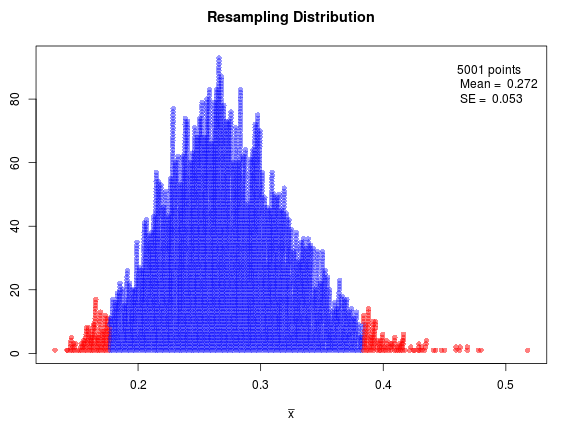
\includegraphics[width=.5\linewidth]{../plots/arsenicCIplot.png}}
\end{key}

Explain how one dot on the plot was created and what it represents in
the context of the problem.
\begin{students}
  \vspace{1cm}
\end{students}
\begin{key}
  {\it One dot was created by sampling with replacement from the
    original data 19 times.  The mean level of arsenic concentration
    in the toenails of the resample is plotted.}
\end{key}

\item \label{SE2ci} Create a 95\% confidence interval using margin of
  error $ME =  2.11  \times SE$.
\begin{students}
  \vspace{1cm}
\end{students}

\begin{key}
  {\it $ 0.272 \pm 2.11(0.053) = (0.16, 0.38)$ ppm}
\end{key}

\item  \label{percentile95} Create a 95\% confidence interval using
  the bootstrap   Percentile Method.
\begin{students}
  \vspace{1cm}
\end{students}

\begin{key}
  {\it $ (0.177, 0.383)$ ppm}
\end{key}

\item  How similar are the confidence intervals in \ref{percentile95}
  and \ref{SE2ci}?
\begin{students}
  \vspace{1cm}
\end{students}

\begin{key}
  {\it Pretty close, the percentile one is a bit higher on both ends
    than the 2.1SE interval.}
\end{key}


\item \label{percentile90}Would you expect a 90\% confidence interval
  to be wider or narrower?  Explain, then give a 90\% (percentile)
  confidence interval.
\begin{students}
  \vspace{2cm}
\end{students}

\begin{key}
  {\it Narrower, we need to capture fewer dots, so we can move in.
    (0.191, 0.365)} 
\end{key}

\item  Interpret the 90\% confidence interval from \ref{percentile90}.
\begin{students}
  \vspace{2cm}
\end{students}

\begin{key}
  {\it We are 90\% confident the true average arsenic level in
    toenails for new Hampshire residents  with a private well is
    between 0.191 and 0.365 ppm. }
\end{key}
\end{enumerate}


{\bf The Second Research Question}: Is the mean arsenic level
for New Hampshire residents with a private well above the 0.15 threshold? 


  There are two possibilities for why the sample average
was 0.272.  List them here and label them as the null and alternative
hypotheses also write the null and alternative in notation.\\
$H_0:$ 
\begin{students}
  \vspace{1cm}
\end{students}
\begin{key}
  {\it   $ \mu = 0.15$:  The water is, on average safe, so we've just
  observed an unusually high sample.}
\end{key}

$H_a:$
\begin{students}
  \vspace{1cm}
\end{students}
\begin{key}

  {\it  $ \mu > 0.15$  The water is, on average, dangerously high in arsenic.}
\end{key}

Is the alternative hypothesis right-tail, left-tail, or two-tail?
\begin{students}
  \vspace{1cm}
\end{students}

\begin{key}
  {\it Right tailed.}
\end{key}

We can simulate the behavior of arsenic concentrations in New
Hampshire ground water if we assume the null hypothesis which gives a
specific value for the mean.  The two key ideas when creating the
reference distribution are:
\begin{itemize}
\item 
 The resamples must be consistent with the null hypothesis.
\item 
 The resamples must be based on the sample data.
\end{itemize}

  We can use cards like we did for the CI above,
but we have to change the values so that they are consistent with the
null, $\mu = 0.15$.

\begin{enumerate}
\setcounter{enumi}{16}
\item How you could modify the sample data so as to force the null
  hypothesis to be true without changing the spread?  (Do not spend
  more than 2 minutes on this question.)
\begin{students}
  \vspace{2cm}
\end{students}

\begin{key}
  {\it  AWV, but if they have read/if you have lectured on this, they
    should know to shift the data to be centered on the null value,
    then resample.} 
\end{key}

% \item Next we will simulate one repetition of the 19 toenail values
%   collected by creating a deck of 19 cards to simulate what the data
%   would look like {\bf if the null hypothesis} were true.
%     \begin{enumerate}
%     \item  What is the null value in this study?
% \begin{students}
%   \vspace{2cm}
% \end{students}

% \begin{key}
%   {\it 0.15}
% \end{key}
\item  \label{shift}How far is the sample mean from this null value?
\begin{students}
  \vspace{2cm}
\end{students}

\begin{key}
  {\it 0.272 – 0.15 = 0.122 above the mean}
\end{key}

\item We need to shift the original data so that is it centered on the null
      value. 
      Subtract the value from (b) from each of the data numbers to
      get:


\begin{center}
\begin{tabular}{|r|r|r|r|r|r|r|r|r|r|} \hline
-0.003 &-0.004 &-0.023 &-0.004 &0.153 &0.236 &-0.042 &0.036 &0.188 &-0.017
\\ \hline
-0.049 &0.710 &0.395 &0.729 &0.147 &0.311 &0.019 &0.013 &0.053
& \\ \hline
\end{tabular}  
\end{center}
      What is the mean of the above values? Why do we want this
      to be the mean?
\begin{students}
  \vspace{1cm}
\end{students}

\begin{key}
  {\it 0.15, because this is the null value. }
\end{key}



\item Now we want to resample the shifted values. To speed up the
  process, we use \fbox{ Test} option under \fbox{One Quant} at
  \webAppURLFrst . You should have already loaded the data, but if
not, go back to \fbox{Input Data} and select the preloaded
\fbox{Arsenic} data.

  \begin{itemize}
    \item Above the main plot, {\bf change the value for the null
      hypothesis} to the one in our null.  (the just barely safe level)
      The software will shift the data to have this mean.
   \end{itemize}

    Look at the box on the left labeled {\sf Original Sample}.
       Does the mean match your answer to \ref{xbar}?  If not, consult
       with your instructor! 
\begin{students}
  \vspace{1cm}
\end{students}

\begin{key}
  {\it Look for data entry errors. }
\end{key}

\item   What is the statistic from the first  resample? (Click the
  blue dot  to see.)
\begin{students}
  \vspace{1cm}
\end{students}

\begin{key}
  {\it AWV}
\end{key}



\item Explain in the context of the problem what the one dot on the
  main plot represents. 
\begin{students}
  \vspace{1cm}
\end{students}

\begin{key}
  {\it The (resample) mean arsenic concentration in toe nails of 19
    New Hampshire residents who use a private well if the true arsenic
    concentration is 0.15 (right at the edge of being  hazardous) }
\end{key}
\item Generate 5000 or more randomization samples.  Copy the summary statistics and
the plot of the randomization distribution below
\begin{students}
  \vspace{4cm}
\end{students}

\begin{key}
  {\it 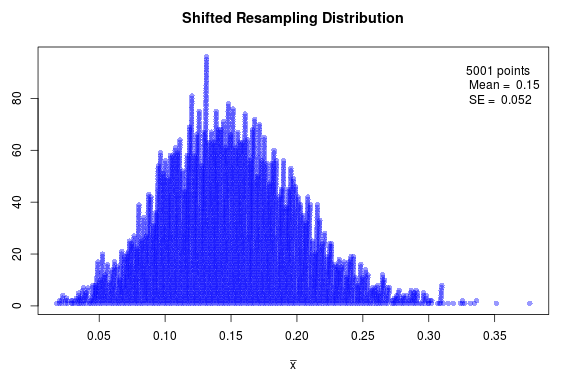
\includegraphics[width=.5\linewidth]{../plots/arsenicNullDistn.png}}
\end{key}


\item 
 Where is the distribution centered?  Why does that make sense?
\begin{students}
  \vspace{1cm}
\end{students}
\begin{key}
  {\it Again, centered at 0.15, because this is the null value. }
\end{key}

Remember why we conducted this simulation: to assess whether the
observed result (mean of 0.272) would be unlikely to occur by chance
alone if the ground water in New Hampshire is not hazardous. 

\item Locate the observed result on the randomization distribution.
  Does it appear to be likely or unlikely to occur under the null
  hypothesis?  Explain your reasoning.
\begin{students}
  \vspace{1cm}
\end{students}

\begin{key}
  {\it Pretty fair in the right tail.  Appears unlikely to occur under
    the null hypothesis. } 
\end{key}

\item \label{pval13}Just how unlikely is the observed result?  Calculate your
  p-value using the web app and the appropriate direction and cutoff value.
\begin{students}
  \vspace{1cm}
\end{students}

\begin{key}
  {\it Right tail p-value = 0.016}
\end{key}

 How many  resamples had a mean at least as extreme as the
 observed result?  
\begin{students}
  \vspace{1cm}
\end{students}

\begin{key}
  {\it AWV}
\end{key}

\item How strong is the evidence against the null hypothesis?  Look back to
  the guidelines for assessing strength of evidence using p-values
  given on page \pageref{fig:SOE-pvalue}.
\begin{students}
  \vspace{1cm}
\end{students}

\begin{key}
  {\it p-value = 0.016, which is strong to very strong evidence
    against the null.}
\end{key}
 

{\bf Step 5: Formulate conclusions.}


\item Based on this analysis, what is your conclusion about the
  residents in New Hampshire who own a private well based on this
  study?
\begin{students}
  \vspace{2cm}
\end{students}

\begin{key}
  {\it We have strong evidence that the true mean arsenic level in
    toenails of NH residents drinking from wells is greater than the
    hazardous threshold of 0.15 ppm.} 
\end{key}
\item Can you extend your results to all of New Hampshire residents?
  All New Hampshire residents with a private well?  Explain your
  reasoning.
\begin{students}
  \vspace{4cm}
\end{students}

\begin{key}
  {\it Our evidence does not extend to all NH residents drinking from
    wells because we don't know that this is a representative sample.
   The data does not include people on municipal water systems, so it
   certainly does not extend to all NH residents.} 
\end{key}

\end{enumerate}

\begin{center}
  {\bf Take Home Messages}\vspace{-.1in}
\end{center}

\begin{itemize}
\item We first reviewed building a CI for a single mean.
\item You need to know when to discuss means versus proportions.  If
  the response has two categories, then we deal with proportions.  If
  the response is quantitative, then we estimate and test means.
\item The new twist today was to do a simulation for testing $H_0: \mu
  = \mu_o$ that the mean is some particular value.  We had to modify
  the data to make $H_0$ true, shifting it from its center at $\xb$ to
  be centered at $\mu_o$.  Then we resampled it as if for a bootstrap
  confidence interval, and located the observed statistic ($\xb$) to
  see how far out in the tails it was (the p--value).

 \item 
Questions? What is your summary of this  lesson? \vfill

\end{itemize}



\noindent
{\bf Assignment} \vspace{-.2in}
\begin{itemize}
% \item D2Box 6 is due March 3.
% \item {\bf D2Quiz 7} is due March 7.  Fill it in online.
 %%  We strongly encourage you to get help in the Math Learning Center.
\item Fill in the simulation confidence interval box in column 2 of
  the Review Table.
\item Watch the ``Types of Errors'' video (\# 4 under Unit 2) and Example 8 under Unit 2.
\item Read the next two pages before your next class.
\end{itemize}
  %% Arsenic test of 1 mean  pgs 127-132
 \newpage

\fancyhead[LE,RO]{
   {\it Notes }\\
   {\it Unit \unitNum\   \ Page \thepage }
}
%Intentionally left blank
\phantom{No text here}
\newpage

\fancyhead[LE,RO]{
   {\it \theTopic }\\
   {\it Unit \unitNum\   \ Page \thepage }
}
  \def\theTopic{Reading 14}

\section{Decisions and Justice}

 Read this article about the justice system and the errors that are
 possible when trying a suspect.\\
\url{http://www.intuitor.com/statistics/T1T2Errors.html}  

\begin{center}
  {\bf Important points}
\end{center}

\begin{itemize}
  \item Assumption:
        \begin{itemize}
        \item In the justice system, what assumption is made about a
          defendant's guilt (or innocence)?\vfill
        \item The web page points out the similarities between the
          justice system and statistical hypothesis testing. What is
          the usual assumption in hypothesis testing (which parallels
          the justice system assumption above)?\vfill
        \end{itemize}
  \item Rejecting the assumption:
    \begin{itemize}
      \item In the justice system, what information causes a jury to
      reject the assumption they start with?  What is the standard for
      them to decide to reject it?\vfill
      \item In hypothesis testing, what information is used to reject
        the assumption?  How do we set the acceptable error rate? \vfill
      \end{itemize}
    \item Conclusions:
      \begin{itemize}
      \item In the justice system, if the jury decides it can reject
        the assumption, they find that the defendant is: \vspace{.8cm}
      \item In hypothesis testing that is equivalent to:\vspace{1cm}
      \item If the jury decides to {\bf not} reject the original
        assumption, they find the defendant: \vspace{.8cm}
      \item In hypothesis testing that is equivalent to:\vspace{1cm}
      \end{itemize}
  \end{itemize}
\newpage
    Their quality control example uses the assumption that a batch of
    some product is ``not defective''. Someone would test the batch to
    see if it has any problems, in which case the whole batch would be
    rejected. 

   We have not yet used the normal distribution which they show.  You
   can instead think of the distributions of dots from simulations you
   have seen in our web app. The idea of p-value is the same --
   that a statistic further out in the tail of the distribution gives
   a smaller p-value and is stronger evidence against $H_0$.

   \begin{itemize}
   \item Stronger evidence. Near the bottom of the web page they
     mention two ways we can reduce the chance of both type I and type
     II error. Here they are for the justice example.  Fill in the
     same ideas for the hypothesis testing situation.  
     \begin{itemize}
     \item More witnesses \vspace{1in}
     \item Higher quality testimony. \vspace{1in}
     \end{itemize}
   \end{itemize}
 
 You might like their applet which illustrates how we can reduce the
 chances of error, but it requires java which is not supported on Mac
 devices.    %% pages 133 -136 buff
  \newpage

\fancyhead[LE,RO]{
   {\it Notes }\\
   {\it Unit \unitNum\   \ Page \thepage }
}
%Intentionally left blank
\phantom{No text here}
\newpage


\fancyhead[LE,RO]{
   {\it \theTopic }\\
   {\it Unit \unitNum\  Activity \dayNum \ Page \thepage }
}

 \def\theTopic{Errors }
\def\dayNum{16 }

\section{ On Being Wrong 5\% of the Time}


Our confidence in a 95\% confidence interval comes from the fact that,
in the long run, the technique works 95\% of the time to capture the
unknown parameter.  This leads to an old cheap joke:

{\sf Statisticians are people who require themselves to be wrong 5\%
  of the time.}

We hope that's not really true, but decision making leads to a dilemma:\\
  If you want to never be wrong, you have to always put off decisions
  and collect more data.

Statistics allows us to make decisions based on partial data  while
controlling our error rates.\\
Discuss these situations and decide which error would be worse:\vspace{-.6cm}
\begin{enumerate}
\item A criminal jury will make an error if
      they let a guilty defendant go free, or if
      they convict an innocent defendant.
     Which is worse? Why?
\begin{students}
  \vspace{1.5cm}
\end{students}

\item The doctor gives patients a test designed to detect pancreatic
  cancer (which is usually quite serious).  The test is wrong if:
  it says a healthy patient has cancer (a false positive), or if
  it says a patient with cancer is healthy (a false negative).  Which
  is worse?  Why? 
\begin{students}
  \vspace{1.5cm}
\end{students}

\item  An FAA weather forecaster has to decide if it is too dangerous
   (due to storms or potential icing conditions) to allow planes to
   take off.  What is the cost of grounding a flight? What could
   happen if a flight should have been kept on the ground, but wasn't?  
\begin{students}
  \vspace{2.5cm}
\end{students}



\item  Large chain stores are always looking for locations into which
  they can expand -- perhaps into Bozeman. 
  When would a  decision to open a store in Bozeman  be wrong?\\
  When would a decision to {\bf not} open a store in Bozeman  be
  wrong?\\
  What are the trade-offs?  
\begin{students}
  \vspace{3cm}
\end{students}

\end{enumerate}

\subsection{ Two Types of Error }

Definitions:\vspace{-.6cm}
\begin{itemize}
  \item To reject $H_0$ when it is true is called a Type I error.
  \item To fail to reject $H_0$ when it is false is called a Type II error.
\vspace{-.6cm}
\end{itemize}
To remember which is which: we start a hypothesis test by assuming
$H_0$ is true, so Type I goes with $H_0$ being true. 

This table also helps us stay organized: \hfill
\begin{tabular}{|l|c|c|}\hline
   & \multicolumn{2}{|c|}{Decision:} \\
$H_0$ is:  & Reject $H_0$ & Do not reject $H_0$\\\hline
true & {\em Type I Error} & Correct  \\ \hline
false& Correct & {\em Type II error}   \\ \hline\hline
\end{tabular}



{\bf Which is worse?}

The setup for hypothesis testing assumes that we really need to
control the rate of Type I error.  We can do this by setting our
 significance level, $\alpha$.  If, for example, $\alpha = 0.01$, then
 when we reject $H_0$ we are making an error less than 1\% of the time.
So $\alpha$ is the probability of making an error when $H_0$ is true.

There is also a symbol for the probability of a Type II error,
$\beta$, but it changes depending on which alternative parameter
value is correct. Instead of focusing on the negative (error), we
more often talk about the {\bf power} of a test to detect an effect
which is really present.  Power = $1-\beta$ is the probability of
rejecting $H_0$ when it is false (that's a good thing, so we want
power to be high). 



\begin{center}
  {\bf Justice System and Errors }
\end{center}

In both the justice system and in statistics, we can make errors. In
statistics the only way to avoid making errors is to not state any
conclusion without measuring or polling the entire population.  That's
expensive and time consuming, so we instead try to control the chances
of making an error.  
 

For a scientist, committing a Type I error means we could report a
big discovery when in fact, nothing is going on. (How embarrassing!)
This is considered to be more critical than a Type II error, which happens if
the scientist does a research project and finds no ``effect'' when, in
fact, there is one. Type I error rate is controlled by setting
$\alpha$, the significance level, and only rejecting $H_0$ when the
p-value is less than $\alpha$. 


Type II error is harder to control because it depends on these things:
\vspace{-.2cm}
\begin{itemize}
\item  Sample size.  P--values are strongly affected by sample
  size. With a big sample we can detect small differences.  With small
  samples, only coarse or obvious ones.
\item  Significance level.  The fence, or $\alpha$ (alpha), is
  usually set at .10, .05 or .01 with smaller values requiring
  stronger evidence before we reject the null hypothesis and thus
  lower probability of error.  
\item  The null hypothesis has to be wrong, but it could be wrong just
  by a small amount or by a large amount.  For example if 
   we did not reject the null hypothesis that treatment and
  control  were equally effective,  we could be making a type II
  error.  If in fact,  there was a small difference, it would be
  hard to detect, and if the treatment was far better, it would
  be easy to detect.  This is called the effect size, which is
  [difference between null model mean and an alternative mean] divided
  by standard error.
\end{itemize}


The Power Demo web app lets us try different values to see what size
power we get.  Go to 
\webAppURLFrst\  and click
\fbox{Power Demo} under \fbox{One Quant}.

\begin{center}
  {\bf Try different sample sizes.}
\end{center}
\begin{enumerate}
  \setcounter{enumi}{4}
  \item  Set SD to 2, Alternative Mean to 1.5, and
    Significance Level to 0.01. Find the power and the effect size for
    each sample size:\\ 
\begin{students}
  \begin{tabular}{ |l|r|r|}\hline
    n & power& effect size\\ \hline
    {\large 4} &&\\ \hline
    {\large 8} &&\\ \hline
    {\large 16} &&\\ \hline
    {\large 32} &&\\ \hline
    {\large 48} &&\\ \hline
  \end{tabular}
\end{students}

\begin{key}
  \begin{tabular}{ |l|r|r|}\hline
    n & power& effect size\\ \hline
     4 &0.085& 0.75\\ \hline
     8 &0.274& 0.75\\ \hline
     16 &0.656& 0.75\\ \hline
     32 &0.958 &0.75\\ \hline
     48 &0.997 &0.75\\ \hline
  \end{tabular}
\end{key}
\item      What happens to power as you increase sample size? Explain why.
\begin{students}
\vspace{2cm} %% 
\end{students}

\begin{key}
  {\it It appears that the distribution under the null and the
    alternative mean get further apart.  In fact, variance decreases
    as sample size increases. }
\end{key}

\begin{center}
  {\bf Try different standard deviations.}
\end{center}

  \item  Set sample size to 16, Alternative Mean to 1.5, and
    Significance Level to 0.01. Find the power and the effect size for
    each Standard Deviation (SD). This SD is the spread of individual
    data points within our sample.\\ 
\begin{students}
  \begin{tabular}{ |l|r|r|}\hline
    SD & power& effect size\\ \hline
    {\large 0.4} && \\ \hline
    {\large 1} &&\\ \hline
    {\large 2} &&\\ \hline
    {\large 3} &&\\ \hline
    {\large 4} &&\\ \hline
  \end{tabular}
\end{students}

\begin{key}
  \begin{tabular}{ |l|r|r|}\hline
     SD & power& effect size\\ \hline
    {\large 0.4}&1.00& 3.75\\ \hline
    {\large 1}  &0.999&1.5\\ \hline
    {\large 1.5}&0.856&0.938\\ \hline
    {\large 2}  &0.656&0.75\\ \hline
    {\large 3}  &0.307&0.5\\ \hline
  \end{tabular}
\end{key}
\item      What happens to power as you increase standard deviation? Explain why.
\begin{students}
\vspace{2cm} %% 
\end{students}

\begin{key}
  {\it It appears that the distribution under the null and the
    alternative mean get closer together.  In fact, variance increases
    as SD increases. }
\end{key}


\begin{center}
  {\bf Try different alternative means.}
\end{center}

  \item  Set sample size to 16, SD to 2, and
    Significance Level to 0.01. Find the power and the effect size for
    each Alternative Mean.\\ 
\begin{students}
  \begin{tabular}{ |l|r|r|}\hline
    Alternative Mean & power& effect size\\ \hline
    {\large 0.4} && \\ \hline
    {\large 0.8} &&\\ \hline
    {\large 1.2} &&\\ \hline
    {\large 1.6} &&\\ \hline
    {\large 2.4} &&\\ \hline
  \end{tabular}
\end{students}

\begin{key}
  \begin{tabular}{ |l|r|r|}\hline
     Alt. Mean & power& effect size\\ \hline
    {\large 0.4} &0.079& 0.25\\ \hline
    {\large 0.8} &0.307&0.5\\ \hline
    {\large 1.2}&0.656 &0.75\\ \hline
    {\large 1.6}&0.903 &1.00\\ \hline
    {\large 2.4}&0.999 &1.5\\ \hline
  \end{tabular}
\end{key}
\item      What happens to power as you increase the alternative mean? Explain why.
\begin{students}
\vspace{2cm} %% 
\end{students}

\begin{key}
  {\it As the alternative mean increases, it gets easier to
    distinguish the two means, and hence easier to reject $H_0$ which
    implies greater power.  }
\end{key}

\item Look at the effect sizes in the last two tables.
    How do SD and Alternative Mean work together to determine power? 
\begin{students}
 \vspace{2cm}
\end{students}

\begin{key}
  {\it     Larger effect for same SD means more power, lower SD for same
    effect means more power.  In general, larger effect and lower
    SD means more power. A given effect size has the same power (for
    fixed $n$) no matter what SD and Alternative Mean we have.}
\end{key}


\begin{center}
  {\bf Try different significance levels.}
\end{center}

  \item  Set sample size to 16, SD to 3, and
    Alternative mean to 1. Find the power and the effect size for
    each significance level ($\alpha$).\\ 
\begin{students}\hline
  \begin{tabular}{ |l|r|r|}\hline
    $\alpha$ & power& effect size\\ \hline
    {\large 0.01} && \\ \hline
    {\large 0.03} &&\\ \hline
    {\large 0.05} &&\\ \hline
    {\large 0.07} &&\\ \hline
    {\large 0.10} &&\\ \hline
  \end{tabular}
\end{students}

\begin{key}
  \begin{tabular}{ |l|r|r|}\hline
    $\alpha$ & power& effect size\\ \hline
    {\large 0.01}&0.54 & 0.667\\ \hline
    {\large 0.03}&0.734 &0.667\\ \hline
    {\large 0.05}&0.816 &0.667\\ \hline
    {\large 0.07}&0.862 &0.667\\ \hline
    {\large 0.10}&0.905 &0.667\\ \hline
  \end{tabular}
\end{key}

  \item    In which direction does power change when we increase the
    significance level?  
\begin{students}
 \vspace{3cm}
\end{students}

\begin{key}
  {\it     It would increase (power and significance level change in the
    same direction). }
\end{key}

\begin{center}
  {\bf Planning a new study}
\end{center}
  \item   Suppose that we are planning to do a study of how energy
    drinks effect RBAN scores similar to the study we read about in
    Activity 14.  From previous data, we have an estimate of standard
    deviation of 3.8. We plan to use a significance level of $\alpha =
    .05$, and want to be able to detect an increase in mean RBAN score
    of 2 with 90\% power.   How large must our sample size be?
\begin{students}
 \vspace{1cm} %%
\end{students}

\begin{key}
  {\it  33}
\end{key}


      If we choose $\alpha = .01$, how large a sample is needed?
\begin{students}
 \vspace{1cm}
\end{students}
\begin{key}
\ \ \   {\it 50}
\end{key}

  \item  Now suppose that we are using a memory test used to study
    sleep deprivation.  Historical data 
    provides an estimate of SD = 13.  We want to use $\alpha = .05$ and
    need to detect a decrease in mean score (when people are sleep
    deprived) of 6 with 80\% power.  
    How large a sample is needed? 
\begin{students}
 \vspace{1cm} %%
\end{students}

\begin{key}
  {\it  31}
\end{key}


    If we want to limit the chance of Type II error to 10\% or less,
    how large a sample size is needed? 
\begin{students}
 \vspace{1cm}\\
\end{students}

\begin{key}
  {\it  Type II = 1--power so we want more than 90\% power.  Need 43
      people. }
\end{key}
\item Suppose we do another study on energy drinks with alcohol using
  Control and REDA.  This time we test hand-eye coordination using
  $H_0:\ \mu_{control} = \mu_{REDA}$ versus alternative  $H_a:\
  \mu_{control} > \mu_{REDA}$.
  \begin{enumerate}
  \item What would be a Type I error in this context? 
\begin{students}
 \vspace{3cm}\\
\end{students}

\begin{key}
  {\it   To conclude that there is a difference in mean coordination between the
    two treatments when, in fact, REDA has no effect on coordination scores. }
\end{key}
  \item What would be a Type II error in this context? 
\begin{students}
 \vspace{5cm}\\
\end{students}

\begin{key}
  {\it  To fail to find a difference in mean coordination between the
    two treatments when, in fact, REDA lowers coordination scores. }
\end{key}
  \end{enumerate}

\end{enumerate}


\begin{center}
  {\bf Take Home Message} \vspace{-.6cm}
\end{center}
\begin{itemize}
  \item Errors happen.  Use of statistics does not prevent all errors,
    but it does limit them to a level we can tolerate. We have labels
    for two types of error.
  \item The talk about probability of  error is based on the sampling
    distribution assuming random assignment of treatments or random
    sampling. It's really a ``best case'' scenario, because there
    could be other sources of error we have not considered.  For
    example, we could have not sampled from some part of the
    population, or we could have errors in our measuring tools.
  \item If you are designing a study, you might need to consult a
    statistician to help determine how large a sample size is
    needed. You'll need to decide what $\alpha$ to use, what the
    underlying variation is ($\sigma$), and how large a difference you
    need to detect with a certain level of power.
 \item 
  Questions? Summarize the  lesson. 
\end{itemize}\vfill



\noindent
{\bf Assignment} \vspace{-.2in}
\begin{itemize}
% \item  D2Quiz 7 is due March 7. 
% \item {\bf D2Box 7} is due March 10.
%     Turn it in as a pdf file in the Drop Box on D2L.
 %%  We strongly encourage you to get help in the Math Learning Center.
\item Read the next two pages before your next class.
\item Watch the ``Correlation and Regression'' video (\# 5 under Unit 2).
\end{itemize}
  %% Errors pgs 137-142
 \newpage

\fancyhead[LE,RO]{
   {\it Notes }\\
   {\it Unit \unitNum\   \ Page \thepage }
}
%Intentionally left blank
\phantom{No text here}
\newpage

\fancyhead[LE,RO]{
   {\it \theTopic }\\
   {\it Unit \unitNum\   \ Page \thepage }
}
  \def\theTopic{Reading 15}

\section{Correlation and Regression - Reading}

Watch the ``Correlation and Regression'' video at ??


\begin{center}
  {\bf Important Points}
\end{center}

\begin{itemize}
\item What type of plot is used to show the relationship between two
  quantitative variables?\vspace{2cm}
\item What does correlation measure?\vspace{2cm}
\item What are possible values for correlation?  \vspace{2cm}
\item What symbol is used for population correlation?  for sample
  correlation? \vspace{2cm}  
\item What values for correlation indicate strong (weak) linear
  association?\vspace{2cm} 
\item  What symbols are used for the true parameters: intercept and
  slope in a regression model?\vspace{2cm}
\item  What symbols are used for the sample statistics: intercept and
  slope of the least squares line? \vspace{2cm}
\item  What is a residual? Which residuals are negative? positive?\vspace{2cm}
\item  We found the estimated least squares line to be
      $\widehat{mpg} = 51.6-0.0073 \times{weight}$ 
      \begin{itemize}
      \item Interpret the slope.\vspace{2cm}
      \item What is the predicted MPG if of a car weighing 2350 pounds? \vspace{2cm}
      \item What is the residual if $y = 46$ and $x = 2350$?\vspace{2cm}  
      \end{itemize}
\item Is it possible to have a negative slope and a positive
  correlation between two quantitative variables? Explain.\vspace*{\fill}
\end{itemize}
   %%  p 143-146  buff
  \newpage

\fancyhead[LE,RO]{
   {\it Notes }\\
   {\it Unit \unitNum\   \ Page \thepage }
}
%Intentionally left blank
\phantom{No text here}
\newpage


\fancyhead[LE,RO]{
   {\it \theTopic }\\
   {\it Unit \unitNum\  Activity \dayNum \ Page \thepage }
}
 \def\theTopic{Correlation/Slope }
\def\dayNum{17 }


\section{Attraction and Age}

\begin{center}
{\bf {Or: Who Looks Good to You?}}
\end{center}


Christian Rudder works for the dating web site OKcupid, and has
written a book, {\it Dataclysm} about some surprising data 
collected from the web site.

As an example, here are plots he gives for women and for men.
The horizontal axis is the age of the man or woman being
interviewed. The vertical axis is the age which they think looks most
attractive in the opposite sex.\vspace{-.5cm}

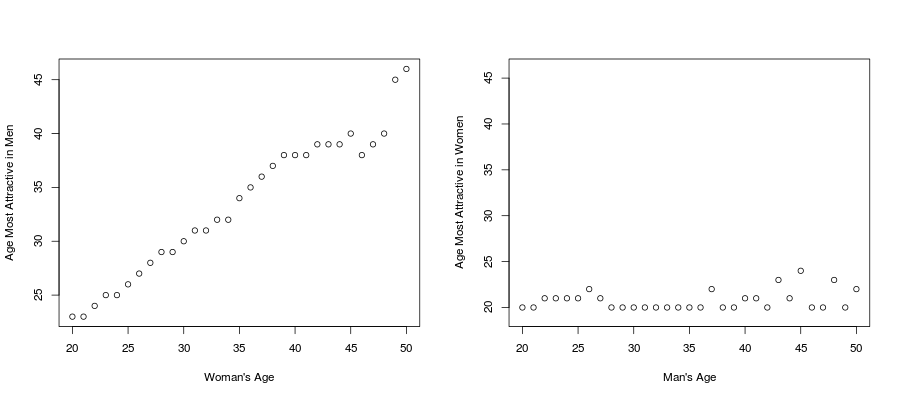
\includegraphics[width=\linewidth]{../plots/attractiveAges.png}

There are clearly big differences between men and women, so we want to
describe them with statistics.\vspace{-.5cm}
\begin{enumerate}
  \item Suppose you're talking to a friend over the telephone, and
    you need to explain  that the same two variables
    have a different relationship for women than for men. How would you
    describe the two plots? 
\begin{students}
 \vspace{2cm}      
\end{students}

\begin{key}
  {\it  I'm hoping for some talk about fitting a line or about slope
    or correlation.}
\end{key}

\item What statistical summaries differ in the two plots?
\begin{students}
 \vspace{2cm}      
\end{students}

\begin{key}
  {\it  Means of the y variable certainly differ,  but again I hope
    they think of slope  or correlation. }
\end{key}



\item As a review, in Algebra class you would have learned an equation
  for a linear relationship between $x$ and $y$.  What letters did you
  use for slope and intercept?  What does ``slope'' mean?  What does
  ``intercept'' mean?
\begin{students}
 \vspace{2cm}      
\end{students}

\begin{key}
  {\it $m$ for slope = rise over run?, $b$ for intercept = $y$ value
    when $x=0$. Other answers are possible.}
\end{key}


  In Statistics, we use the following equation for a ``true'' regression  line:
  $$ y = \beta_0 + \beta_1 x + \epsilon  $$
  and when we estimate the line we add hats to the parameters,
  $\beta_0$ and $\beta_1$, and also to the left side to say we have an
  estimated response, $\hat{y}$.
  $$ \hat{y} = \hat{\beta}_0 + \hat{\beta}_1 x$$
\item Estimate the  slopes for the two plots above.\\
     Hint: For each plot take a nice range of ages on the x axis, say
    from 20 to 40, and guess how much the line changes from the lower
    $x$ value to the upper one.  The change in $y$ over change in $x$
    gives the slope estimate.
\begin{students}
 \vspace{2cm}      
\end{students}

\begin{key}
  {\it Women: as x goes from 20 to 45, I'd guess y goes from 25 to 40,
    so slope is roughly 15/25 = .6\\
        Men: going from 20 to 50 might raise the $y$ value by 2 so
        slope estimate could be 2/30 = 0.067  }
\end{key}

\item Interpret your estimated slopes.
\begin{students}
 \vspace{2cm}      
\end{students}

\begin{key}
  {\it  As women's age goes up one year, the age of her most
    attractive man increases by about 0.67 years.  For men, as his age
  increases by one year, the age of his most attractive woman goes up
  by 0.07 years.}
\end{key}



\subsection { Slope}


\item  In Algebra, a line is a collection of points satisfying an
     equation. In Statistics we start with data and have to find a good
     line to represent the relationship between two variables.  When
     there is a lot of scatter in the points, many lines look
     reasonable.  Go to 
     \url{http://www.rossmanchance.com/applets/RegShuffle.htm}
     to see data on people's foot length versus height.
     \begin{enumerate}
     \item Is this a linear relationship? \\
     \item Positive or Negative? \\
     \item Strong, Moderate, or Weak? \\
     \item Guess the correlation, then check with the button below the
       plot.
     \end{enumerate}
\begin{key}
 Linear, positive, moderately strong.      $ r = .71$  
\end{key}

   We'll use this app for the rest of this activity.

\item Click {\sf Show Movable Line:} \fbox{$\surd$} and move the
  center by dragging the large green square in the middle and adjust
  the slope by dragging either end of the line up or down.  Get the
  line which you think best fits, write its equation here:
  $$ \widehat{\mbox{height}} = \_\_\_\_ + \_\_\_\_ \times \mbox{footlength}$$
\begin{students}
 \vspace{.2cm}      
\end{students}

\begin{key}
  {\it I got intercept 40.5, slope = 0.94}
\end{key}
\item Click {\sf Show Regression Line:} \fbox{$\surd$} and write the
  equation here:
  $$ \widehat{\mbox{height}} = \_\_\_ + \_\_\_ \times
  \mbox{footlength}$$
\begin{key}
  {\it $ \widehat{y} = 38.3 + 1.03 x$}
\end{key}
\begin{enumerate}
  \item Was your slope too large? too small? about right? 

  \item What height does this line give for a person whose foot length
    is 0?\vspace{.9cm}\\

    (This is an example of {\bf extrapolation}: predicting $y$ for an $x$ value
    outside the range of observed $x$'s.)
\end{enumerate}


\item  Let's see how much we can change slope and correlation by
  adding just one more point.  Give it a new ``x''  value of 60 cm.
  Pick a ``y'' value which you think will change the general pattern
  we see between length and height. Can you get the correlation to go
  close to zero?  I'm not having luck with ``move observations'' but
  you can edit the last line of data to try  new ``y'' values  until
  you get a correlation of about zero.  
  \begin{enumerate}
  \item 
  What are the coordinates of
  the added point?
\begin{students}
 \vspace{1cm}      
\end{students}

\begin{key}
  {\it (50, 56.4) has $r = 0.001$}
\end{key}
\item 
  Now what is the slope of the regression line? 
\begin{students}
 \vspace{1cm}      
\end{students}

\begin{key}
  {\it Close to 0 as well, I got a weird underflow problem, but it's
    about 0.0009}
\end{key}
\item Is correlation resistant to outliers?  Is slope? Explain.
  \begin{students}
 \vspace{1cm}      
\end{students}
\begin{key}
  {\it No.  One outlier completely changed correlation and slope.}
\end{key}
\end{enumerate}
\item Click \fbox{\sf Revert} to go back to the original data. Have it
  show the regression line and the residuals.  You can't see from the
  plot, but points below the line have negative residuals, points
  above the line have positive residuals according to this definition:
$$ \mbox{residual} = \mbox{observed} - \mbox{predicted or } 
       e = y - \hat{y}$$
 \begin{enumerate}
   \item   Which residual is largest?
     Find the (x, y) pair  in the data table associated with that
     point.
\begin{students}
 \vspace{1cm}      
\end{students}

\begin{key}
  {\it (30, 74)}
\end{key}
\item Compute its predicted value using the equation given.  Also
     compute the residual for the one furthest below the line.
\begin{students}
 \vspace{1cm}      
\end{students}

\begin{key}
  {\it (30, 74) has the largest residual of $74 - (38.3 +1.03\times
    30) = 74 - 69.2 = 4.8$.   Smallest comes from (24, 56) with
    predicted value $38.3+1.03\times 24 = 63.02$ so its residual is
    $56 - 63.02 = -7.02$ }
\end{key}
   \item Now click {\sf Show Squared Residuals}.  These are important
     because we are using the ``Least Squares'' line. It picks slope
     and intercept to minimize the sum of all the squared residuals.
     Write down SSE (sum of squared errors). 
\begin{students}
 \vspace{1cm}      
\end{students}

\begin{key}
  {\it 235}
\end{key} 
Any other line will have larger SSE.
\end{enumerate}

  \subsection{ Correlation}

  \item {\bf Correlation} measures the strength and direction of a {\bf
  linear} relationship between two quantitative variables. It is a
unit-less number between -1 and 1 with zero meaning ``uncorrelated'' and
1 or -1 meaning perfect correlation -- points fall right on a
line. The sample correlation is called $r$, and the true correlation
is $\rho$, the Greek letter ``rho''. 
 The sign  of the correlation tells us if the one variable
 increases as the other does (positive) or decreases (negative).

   Go to  \url{http://www.tylervigen.com/ } and find a
    ``spurious'' correlation which has correlation coefficient, $r$ less
    than -0.90 and one that has $r > 0.99$.  Here are the two
    variables plotted without year ( a lurking variable).\\
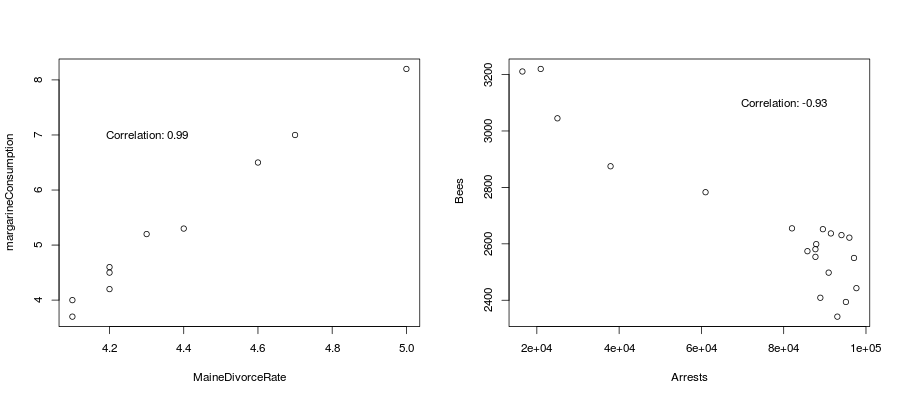
\includegraphics[width=\linewidth]{../plots/spuriousCorr.png}
    The point here is that if you search through lots of variables,
    you can find pairs that increase in the same way, or oppositely.

    Just to show you found the site, what variables are in the first
    plot, and what is their correlation?
\begin{students}
 \vspace{1cm}      
\end{students}

\begin{key}
  {\it  US spending on Science, Space, Technology has correlation 0.99
  with Suicides by hanging, suffocation, and drowning.}
\end{key}

\item Why are the values on that page called ``spurious''?
\begin{students}
 \vspace{1cm}      
\end{students}

\begin{key}
  {\it Because there is no reason that the two variables should be
    correlated. }
\end{key}

\item Correlations in the following plot are either 0.96 or 0.56.
  Which is which?\\
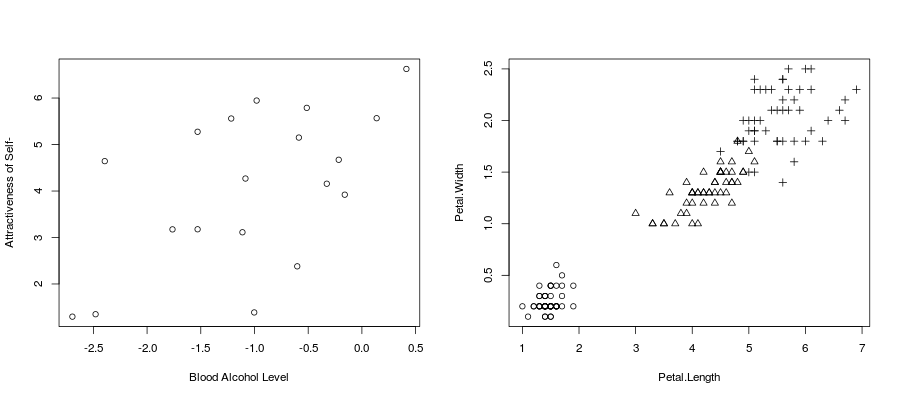
\includegraphics[width=\linewidth]{../plots/realCorr.png}
\begin{students}
 \vspace{1cm}      
\end{students}

\begin{key}
  {\it 0.56 - attractiveness and BAL, and 0.96 - petals}
\end{key}

  The first is data recreated from summary stats given for a study of
  how attractive men felt they were and their blood alcohol level (log
  scale, so negative numbers do make sense).
  The second shows measurements of iris petals. The clusters are for
  three different species. Within
  species correlations are quite different: 0.33, 0.79 and 0.32, but
  with all the data, correlation is higher. 

\item Look back at the Age-Attraction plots from OKcupid.
  Guess what those correlations are for women and for men.
\begin{students}
 \vspace{1cm}
\end{students}

\begin{key}
  {\it 0.98  and 0.28}
\end{key}

\item Correlation contest:\\
  Go to
  \url{http://www.rossmanchance.com/applets/GuessCorrelation.html}.
  Click \fbox{$\surd$} {\sf Track Performance}, then each member of your
  group guesses correlation for 5 \fbox{New Sample}s. (Click \fbox{\sf
    Reset} between each person.)  The first plot
  below {\sf Track Performance} tells you the correlation between your
  guesses and the true values.  What  is it? What's the best one in
  your group? 
\begin{students} 
\vspace{1cm}\newpage
\end{students}



\end{enumerate}

\begin{center}
  {\bf Take Home Messages:}\vspace{-.4cm}
\end{center}
\begin{itemize}
\item It's not right to speak of the correlation between gender (or any
  categorical variable) and age, or between two categorical variables.
\item It only works for linear relationships.  We can have very strong
  nonlinear association with correlation near zero.
\item Positive relationships mean large values in one variable are
  generally  paired  with large values  in  the other variable
  (and small with small).  Negative relationships pair large with small.
\item Correlation has no units and is restricted to the interval
  (-1,1). Both end of the interval indicate very strong
  correlation. Near zero, we say the two variables are uncorrelated.

\item Neither correlation nor slope are resistant to outliers.  A
  change in one point can completely change these values.
\item Slope of the ``Least Squares'' line is given the label
  $\hat{\beta}_1$ because it estimates the true slope, $\beta_1$.  It is
  related to correlation.  
  $$  \hat{\beta}_1 = r \times\frac{s_y}{s_x}$$
  where $s_y$ is the Standard Deviation (SD) of the responses, and $s_x$ is
  the SD of the explanatory variable.
\end{itemize}




\noindent
{\bf Assignment} \vspace{-.2in}
\begin{itemize}
 \item  D2Quiz 7 is due Oct 20.
 \item {\bf D2Box 8} is due Oct 24.
 %%  We strongly encourage you to get help in the Math Learning
 %%  Center.
\item Watch videos assigned on D2L.
\item Fill in the simulation confidence interval box in column 2 of
  the Review Table.
\item Read the next two pages before your next class.
\end{itemize}

  %% slope corr 5 pgs 148-152  Rossman-CHance
 \newpage

\fancyhead[LE,RO]{
   {\it Notes }\\
   {\it Unit \unitNum\   \ Page \thepage }
}
%Intentionally left blank
\phantom{No text here}
\newpage

\fancyhead[LE,RO]{
   {\it \theTopic }\\
   {\it Unit \unitNum\   \ Page \thepage }
}
  \def\theTopic{Reading 16}

\section{Testing Slope}

Watch this video:  \url{??}


\begin{itemize}
 \item What is the usual null hypothesis for a test of slope? Be sure
   to use the right parameter. \vspace{1.5cm}

 \item What is the alternative hypothesis for the example of taxi tips?\vspace{1.5cm}

 \item What is the equation of the least squares line?\vspace{1.5cm}

 \item If you are heading to NYC, what percentage would you expect to give a
   cabbie as a tip?\\
    (These data are for fares paid with credit cards. If we look at
    fares paid with cash, lots of people gave no tip. Apparently
    people doing 'business lunches' tend to use cards more, and they
    can include the tip as part of the expense, so they are more
    generous.  Answer the question as if you are one of them.) \vspace{2cm}

  % \item Why is the p-value so small?  Compare what you see in the
  %   lower left hand plot with the upper left hand plot. Try clicking
  %   on different points in the right hand plot to see what data
  %   generated the slope seen on the right. \vspace{2cm}

  \item What is the usual null hypothesis for a test of correlation? Be sure
   to use the right parameter. \vspace{2cm}
  \item Explain the null hypothesis in your own words.  What does it
    say about the relationship between the two variables?\vspace{2cm}

  \item What is the alternative hypothesis for the example of taxi tips?\vspace{2cm}

\end{itemize}
\normalsize
   %% Test slope pages 153 - 154 buff

  \newpage
\fancyhead[LE,RO]{
   {\it \theTopic }\\
   {\it Unit \unitNum\  Activity \dayNum \ Page \thepage }
}
 \def\theTopic{Testing Slope = 0 }
\def\dayNum{18 }



\section{ Is Correlation Zero?  Is Slope Zero?}

Recall the plots we started with last time of ``most attractive age'':
\vspace{-.5cm}

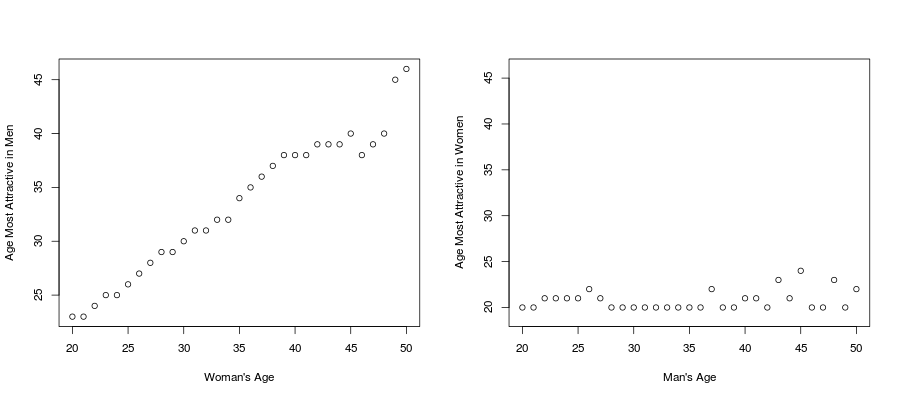
\includegraphics[width=\linewidth]{../plots/attractiveAges.png}

Least squares regression lines:
$$ \mbox{Women: } \hat{y} = 9.02 + 0.70x \mbox{ \hspace{2in}}
   \mbox{Men: } \hat{y} = 19.57 + 0.0343x \mbox{ \vspace{-.7cm}} $$ 
\begin{enumerate}
\item Use the least squares line to estimate what women aged 36.5
  would say is the most attractive age of men?
\begin{students}
 \vspace{1.5cm}      
\end{students}

\begin{key}
  {\it     Plug 36.5 in as the x value and compute $\hat{y} = 34.47$.}
\end{key}

  \item Use the least squares line to estimate what men aged 49.5
    would say is the  most attractive age of women? 
\begin{students}
 \vspace{1.5cm}      
\end{students}

\begin{key}
  {\it     Plug 49.5 in as the x value and compute $\hat{y} = 21.27$.}
\end{key}

\item Discuss this alternative with your group.  Perhaps the age of
  the men really doesn't matter, and we'd be better off estimating
  their preference by using the mean ``most attractive age for women''
  which is $\overline{y} = 20.77$ for all men, just ignoring the men's age.
   Does that seem like a reasonable way to describe the second plot:
   ``men of all ages find 20.8 years to be the most attractive in women''?
  Write down your group's conclusion.
  \begin{students}
 \vspace{2cm}      
\end{students}

\begin{key}
  {\it    I hope they can see some validity in both regression line
    and flat line.}
\end{key}

  BTW: If any of you women over age 23 find this depressing, Rudder
  does say in his book that when men go to search for women on the
  dating site, they do adjust for their own age and ask to see
  profiles of older women if they are older themselves.  % Also, our $y$
  % values are averaged over a bunch of men of the same age. If we used
  % data from individuals, the relationship would be even weaker.


\item Go to the website
  \url{https://jimrc.shinyapps.io/Sp-IntRoStats}
  select \fbox{Two Quant.} and ``Enter Data''. The OKcupid data is
  preloaded as either {\tt WomenRateMen} or {\tt MenRateWomen}. Use
  the men's rating of women for now.

Consider this line:
  {\it  $\widehat{mostAttrWomen} = 20.77 + 0 \times $ mansAge   }


    \begin{enumerate} 
    \item Where have you seen the intercept estimate before (data
      input page)?

      \item If you plug in any age for men, say 18 or 54, what result
        will you get from this line?
\begin{students}
 \vspace{1.cm}      
\end{students}

\begin{key}
  {\it   20.77    }
\end{key}
      \item What does that say about the relationship between $x$ and
        $y$?
\begin{students}
 \vspace{1.cm}      
\end{students}

\begin{key}
  {\it  $y$ does not depend on $x$  }
\end{key}

      \item What will be the true slope for $y$ based on $x$ if there
        is no relationship?  Use    correct notation.
\begin{students}
 \vspace{1cm}      
\end{students}

\begin{key}
  {\it  $\beta_1=0$   }
\end{key}
      \end{enumerate}
      

\item  If we  want to test the null hypothesis ``no linear
  relationship between men's age and the age of women they find most
  attractive'', what is the null value of the true slope?  Use $\beta_1$ as the
  true slope and fill in the hypotheses.  Use a ``right-tailed''
  alternative because we think ages should go up together.\\
  $H_o:$
\begin{students}
 \vspace{1cm}      
\end{students}
\begin{key}
  {\it  $\beta_1 = 0$   }
\end{key}

  $H_a$
\begin{students}
 \vspace{1cm}      
\end{students}
\begin{key}
  {\it  $\beta_1 > 0$   }
\end{key}

\item We need to do a simulation of possible slope values when $H_0$
  is true. If there really is no connection between the two variables,
  $x$, and $y$, what kind of a ``shuffle'' could we do? 
\begin{students}
 \vspace{1cm}      
\end{students}

\begin{key}
  {\it Mix up the pairs in some way. Shuffle all x's and reassign to
    y's or vice versa or shuffle both.  All come out the same.}
\end{key}

\item When you select ``Test'' for these data, a ``Shuffled Data''
  plot appears in the middle of the page. For each $x$ value, there is
  a line from the original (blue) y value to the new shuffled $y$
  value (green).   Does this shuffle follow $H_0$ or $H_a$?  Explain.
\begin{students}
 \vspace{1cm}      
\end{students}

\begin{key}
  {\it  Y's are shuffled. If $H_0$
  is true, then there is no linear association between $x$ and $y$, so
the shuffled data could have occurred just by chance.}
\end{key}

% \item Change Data to Plot. The red line comes from where? 
% \begin{students}
%  \vspace{1cm}      
% \end{students}

% \begin{key}
%   {\it  It's the least squares line from the left-hand plot of the
%     original data.   }
% \end{key}
\item %Run several  shuffles, then several 1000.  
Is the least squares line in the lower plot  flatter or steeper than
the one  in the upper plot?  Is $\hat{\beta}_1$ closer or further
from zero? 
\begin{students}
 \vspace{1cm}      
\end{students}

\begin{key}
  {\it AWV.  generally flatter}
\end{key}

\item  Take at least 1000 shuffles and compute the p-value.  Explain
  which shuffles you are counting based on the plot provided and 
  the original line.
\begin{students}
 \vspace{2cm}      
\end{students}

\begin{key}
  {\it In 10000 shuffles, I had 549 with slope greater than 0.0343, so
  my p--value is 0.055}
\end{key}

\item State your decision and conclusion using $\alpha = 0.05$.
\begin{students}
 \vspace{2cm}      
\end{students}

\begin{key}
  {\it At the $\alpha = 0.05$ significance level we do not reject
    $H_0$, We have only moderate evidence that the true slope between
    men's age and the age of woman they find most attractive is
    greater than zero.  In other words: There is a weak positive
    association between the two variables which is not significant at
    the 0.05 level.}
\end{key}

\item Switch from slope to correlation. What is the sample
  correlation, and what is the p-value for a test of $H_0:\ \rho=0$
  versus $H_a:\ \rho > 0$?.
\begin{students}
 \vspace{1cm}      
\end{students}

\begin{key}
{\it $r = 0.287$ and the p-value is the same.}
\end{key}

\item Now test to see if slope is zero when we compare women's age
  (now this is $x$) to the age of men they find most attractive (our
  new $y$). Again use a ``right-tailed'' alternative.  
  \begin{enumerate}
  \item State the hypotheses.\\
  $H_o:$
\begin{students}
 \vspace{1cm}      
\end{students}
\begin{key}
  {\it  $\beta_1 = 0$   }
\end{key}

  $H_a$
\begin{students}
 \vspace{1cm}      
\end{students}
\begin{key}
  {\it  $\beta_1 > 0$   We don't expect a negative relationship.}
\end{key}

  \item Go back to ``Enter Data'' and load the women's data.  What is
    the equation of the least squares line?
\begin{students}
 \vspace{1cm}      
\end{students}

\begin{key}
  {\it $\widehat{mostAttrMen}$ = 9.02 + 0.6972 x womansAge}
\end{key}


  \item Create 1 random shuffle of the data.  Explain (yes, again --
    it's important)  what is being shuffled. 
\begin{students}
 \vspace{1.8cm}      
\end{students}

\begin{key}
  {\it Use the same woman's ages from 20 to 50. Shuffle the ages of the
    men each woman finds most attractive ($y$)}
\end{key}

  \item Compute the p--value and interpret it.
\begin{students}
 \vspace{1cm}      
\end{students}

\begin{key}
  {\it I get 0. In 10000 shuffles, none was as extreme as the slope we
    observed. The p-value is the probability of seeing a slope this
    far above 0 if, in fact, woman's age ($x$) and most attractive
    man's age ($y$) are really unrelated (true $\beta_1=0$).}
\end{key}


\item State your decision and conclusion using $\alpha = 0.05$.
\begin{students}
 \vspace{2cm}      
\end{students}

\begin{key}
  {\it At the $\alpha = 0.05$ significance level we  reject
    $H_0$, We have super strong evidence that the true slope between
    women's age and the age of man they find most attractive is
    greater than zero.  In other words: There is a very strong positive
    association between the two variables which is significant at
    the 0.05 level.}
\end{key}

 
\item Switch from slope to correlation. What is the sample
  correlation, and what is the p-value for a test of $H_0:\ \rho=0$
  versus $H_a:\ \rho > 0$?.
\begin{students}
 \vspace{1cm}      
\end{students}

\begin{key}
{\it $r = 0.982$ and the p-value is the same.}
\end{key}
  \end{enumerate}

  
\item Are the men and women shown in these plots a random sample from
  a larger population?  Are they representative of some larger population?
\begin{students}
 \vspace{2cm}      
\end{students}

\begin{key}
  {\it No.  The data are averaged across each age, and we can't say
    that the people using this dating site represent a larger
    population of singles.}
\end{key}

\item Was some  treatment  randomly assigned?
\begin{students}
 \vspace{1.5cm}      
\end{students}

\begin{key}
  {\it No.  The ``explanatory'' ages ($x$ values) were observed for
    each person, not assigned.} 
\end{key}

\item What is the scope of inference?
\begin{students}
 \vspace{1.5cm}      
\end{students}

\begin{key}
  {\it We can only say there is ( for women,  is not for men)
    evidence of association in these samples of singles.} 
\end{key}

\item Write a report on the two hypothesis tests we just did. \vfill
\end{enumerate}
 

\begin{center}
  {\bf Take Home Messages:}\vspace{-.4cm}
\end{center}
\begin{itemize}
  \item A slope of zero is very ``special'' in that it says we would
    predict the same value for the response, $\hat{y}$ for all values
    of $x$.  That means that there is no linear relationship between
    the two variables.
  \item The OKCupid data gives us one example where slope is close to
    zero and another where slope is far from zero.  Our conclusions
    should be quite different.
  \item The mechanics of computing p--value have not changed.  We
    assumed $H_0$ was true, and created shuffled data consistent with
    $H_0$.  For each dataset, we computed a slope, and plotted a
    histogram for slopes under $H_0$. P--value counted the number of
    times a slope was as or more extreme as the one we observed
    divided by the number of shuffles.  The only difference is that we
    had the computer find slopes instead of proportions or means.  You
    can easily click the correlation button to get a test of $H_0:\ \
    \rho = 0$. P--values will agree with the test for slope = 0.
  \item How did we shuffle the data under $H_0$ to get other possibles
    slopes or correlations?
  \item What is plotted for one shuffle?
 \item 
 Questions? How would you summarize the lesson? \vspace*{\fill}

\end{itemize}


\noindent
{\bf Assignment} \vspace{-.2in}
\begin{itemize}
% \item  D2Quiz 8 is due March 21.
% \item {\bf D2Box 8} is due March 24.  Turn it in as a pdf file in the
%   Drop Box on D2L. 
 %%  We strongly encourage you to get help in the Math Learning Center.
\item Fill in the top five boxes in the rightmost column   of
  the Review Table.
\item Watch videos assigned on D2L.
\item Instead of a reading for the next class, your assignment is to
  find an example of a simple linear regression model which is
  applicable to an area that interests you.  Be ready to present it to
  your group:  the variables, the estimated coefficients, and the
  meaning of the slope estimate.  Do they provide any evidence that
  the slope is not zero?
\end{itemize}

  %% test slope:  155-160
  \newpage

\fancyhead[LE,RO]{
   {\it Notes }\\
   {\it Unit \unitNum\   \ Page \thepage }
}
%Intentionally left blank
\phantom{No text here}
\newpage

 \newpage
\fancyhead[LE,RO]{
   {\it \theTopic }\\
   {\it Unit \unitNum\  Activity \dayNum \ Page \thepage }
}

           %%  no reading U2-R17 -- they find a regression example.
 \def\theTopic{Regression Examples }
\def\dayNum{19 }

\section{ Regression Examples}

\begin{enumerate}
\item One hundred homes\footnote{Dr. Roger
    Woodard, NCSU } were randomly \vspace{-.24in}\\ 
  \begin{minipage}{.35\linewidth} 
  sampled from a database of all
  homes in Wake County, NC.  We
  have the square footage of each home and an estimated (2008) value of
  the property.  The plot shows 98 homes with value less than \$1
  million.  \vspace*{1in}
  \end{minipage}\hfill
  \begin{minipage}{.60\linewidth}
    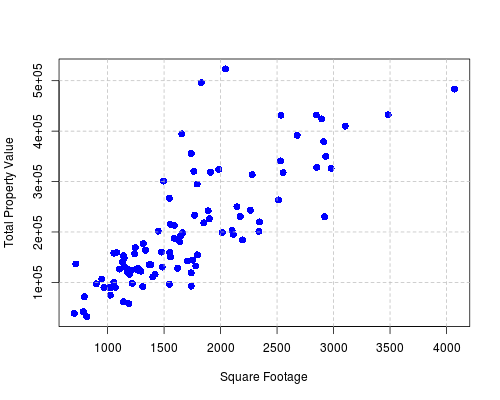
\includegraphics[width = \linewidth]{./plots/WakeCtyHomes.png}
  \end{minipage}
  \item  Describe the relationship (linear or nonlinear? positive or
    negative? strong or weak?) and give a guess at the correlation
    between area and value.
\begin{students}
 \vspace{2cm}\\
\end{students}

\begin{key}
  {\it linear, strong, positive, $r = 0.80$ }
\end{key}

  \item The equation of the least squares line is:
  $$  \widehat{value} =  -30748 + 137\times{sqft}$$
  \begin{enumerate}
  \item Compute the fitted values for homes of size 1000 and 4000 sqft.
\begin{students}
 \vspace{2cm}\\
\end{students}

\begin{key}
  {\it  for 1000: 106252  and for 4000: 517252 }
\end{key}
   \item  Mark the points on the plot and connect them to get the line
     of best fit.  \\
      Note: \verb|1.0+e05| means 1 times $10^5$, or \$100,000.  \vspace{.1in}
   \item The observed value for a 3483 sqft home is  432516.
     Compute predicted price and find the  residual.
\begin{students}
 \vspace{2cm}\\
\end{students}

\begin{key}
  {\it  0.041}
\end{key}
   \item  Two homes in particular do not seem to fit the linear
     relationship very well.  Circle them and theorize: why might they
     have a value other than what the model predicts?  
\begin{students}
 \vspace{2cm}\\
\end{students}

\begin{key}
  {\it Size is only one variable, and it does pretty well by itself,
    but these home might have more amenities or have nicer locations
    than the others.}
\end{key}

\item Interpret the slope estimate. 
\begin{students}
 \vspace{2cm}
\end{students}

\begin{key}
  {\it Each additional square foot of house raises the estimated total
  value by \$137 }
\end{key}


\end{enumerate}


\item Sixteen student volunteers\footnote{ Diez, D.M., Barr, C.D., and
    \c{C}etinkaya-Rundel, M. (2014). {\it Introductory Statistics with
    Randomization and Simulation}
     Exercise 5.28}  at \vspace{-.2in}\\ 
  \begin{minipage}{.35\linewidth}
   Ohio State University were each
  randomly assigned a number of cans of beer to drink.  Thirty minutes
  later, a police officer measured their blood alcohol 
  content (BAC) in grams of alcohol per deciliter of blood. 
  First we'll look at a plot: \vspace*{1in}

  \end{minipage}\hfill
  \begin{minipage}{.60\linewidth}
    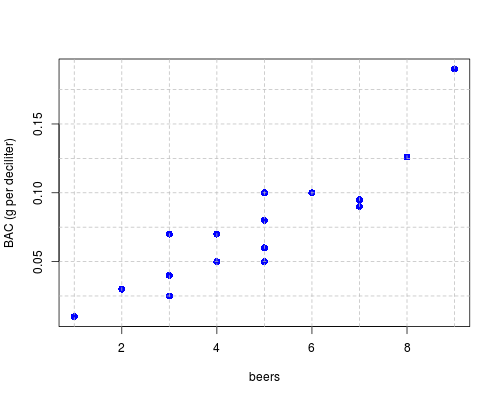
\includegraphics[width = \linewidth]{./plots/beer-BAC.png}
  \end{minipage}
\begin{enumerate}
  \item  Describe the relationship (linear or nonlinear? positive or
    negative? strong or weak?) and give a guess at the correlation
    between beers and BAC. 
\begin{students}
 \vspace{2cm}\\
\end{students}

\begin{key}
  {\it linear, strong, positive, $r = 0.90$ }
\end{key}

  \item The equation of the least squares line is:
  $$  \widehat{BAC} =  -0.013 + 0.018\times{beers}$$
  \begin{enumerate}
  \item Compute the fitted values for 2 and 9 beers.
\begin{students}
 \vspace{2cm}\\
\end{students}

\begin{key}
  {\it  for 2: 0.023  and for 9:  0.149}
\end{key}
   \item  Mark the points on the plot and connect them to get the line
     of best fit. \vspace{.2in}
   \item The observed BAC for the person who drank nine beers was 
     0.190. Compute the residual for the 9 beers person. 
\begin{students}
 \vspace{2cm}\\
\end{students}

\begin{key}
  {\it  0.041}
\end{key}
   \item  The eighth beer drinker had observed BAC of 0.126. Compute
     that residual as well and explain why one residual is negative
     and the other positive.
\begin{students}
 \vspace{2cm}\\
\end{students}

\begin{key}
  {\it  -0.005. This one is negative because it's below the line. The
    9 beers person's point is above the line, so it has a positive residual.}
\end{key}

\end{enumerate}
\item Interpret the slope estimate. 
\begin{students}
 \vspace{2cm}
\end{students}

\begin{key}
  {\it Each beer a person drinks is estimated to increase BAC by 0.018 g/dl}
\end{key}

\item Interpret the intercept estimate. Does its sign make sense?
\begin{students}
 \vspace{2cm}\\
\end{students}

\begin{key}
  {\it A person who has had 0 beers is estimated have BAC of -0.013
    g/dl, which does not make sense. We cannot have negative alcohol
    content in our systems. The SE of this estimate is 0.0123, so it
    is only 1 SE below zero.}
\end{key}
\end{enumerate}\vspace*{\fill}




\end{enumerate}




\noindent
{\bf Assignment} \vspace{-.2in}
\begin{itemize}
\item Check D2L for further assignments. 
\item Review for the exam.
\item Warning: D2Quiz 9 is due Monday, Nov 7. You might not have class
  between the exam and this date, but you will have covered the
  material in a prior class.  Fill it in on D2L.
 %%  We strongly encourage you to get help in the Math Learning Center.
\end{itemize}


  %  beer <- read.csv("beers.csv")
  %  plot(BAC~beers, beer, pch = 16, col = "blue", cex = 1.3, ylab = "BAC (g per deciliter)")
  % abline(h = (1:7)*.025, lty=2, col = "grey")
  % abline(v = 1:9, lty=2, col = "grey")
  % dev.copy(png,file="plots/beer-BAC.png", height = 400, width = 500);dev.off()
  % summary(lm(BAC~beers, beer))
  
 % wakeCty <- read.csv("wakeCtyHomes.csv")
 % names(wakeCty)[c(3,8)] <- c("sqFootage","totalValue")
 % plot(totalValue ~ sqFootage, pch = 16, col = "blue", cex = 1.3, data
 %     = subset(wakeCty, totalValue < 1.0e06), xlab = "Square Footage",
 %     ylab = "Total Property Value") 
 % abline(h=(1:5)*10^5, lty=2, col = "grey")
 % abline(v=(2:8)*500, lty=2, col = "grey")
 % dev.copy(png,file="plots/WakeCtyHomes.png", height = 400, width = 500);dev.off()
 % summary(lm(totalValue ~ sqFootage, data = subset(wakeCty, totalValue
 % < 1.0e06)))
   %% more regression p 161- 163 
 \newpage

\fancyhead[LE,RO]{
   {\it Notes }\\
   {\it Unit \unitNum\   \ Page \thepage }
}
%Intentionally left blank
\phantom{No text here}
\newpage


\fancyhead[LE,RO]{
   {\it \theTopic }\\
   {\it Unit \unitNum\  Activity \dayNum \ Page \thepage }
}

 \def\theTopic{Unit 2 Wrapup }
\def\dayNum{20 }

\section{ Unit 2 Wrapup}

Vocabulary


\begin{itemize}
  \item  Random Sampling
  \item Principles of Designing experiments
  \item  Response and Explanatory variables
  \item  Random Assignment (why do we do it?)
  \item  Lurking Variables
  \item  Causal inference (versus just association)
  \item  Scope of Inference
  \item  Permuting labels, permutation test, randomization test
  \item  Bootstrap process: CI for $\mu$\\
         Percentile method\\
         estimate $\pm t^* SE$
  \item  What points must be included in a statistical report?
  \item  Statistical significance is not the same as importance or practical
    significance.
  \item Interpretation of Confidence Interval
  \item Correlation, Slope. When are they useful? How are they interpreted?
  \item  Type I Error  – probability of this error is limited by
    $\alpha$, the significance level.
  \item  Type II Error.   Power is the probability we (correctly)
    reject the null hypothesis when an alternative is true. Power =  $1-\beta$.
  \item  What settings affect power of a study?
  \end{itemize}
  
  We have built confidence intervals and done hypothesis tests for one
  mean, difference in proportions, difference in two means. And we did
  hypothesis testing for a slope (or correlation) being 0. (Could also
  estimate slope with a CI, but didn't have time).

  \begin{enumerate}
  \item For all studies in Unit 2 consider whether the study was an
    experiment or observational study.  What was the explanatory
    variable? the response?
  \end{enumerate}
  \begin{key}
 \begin{tabular}{|l|c|c|c|}\hline
Study&Experiment?&Explanatory Variable&Response Variable\\ \hline
Study Music &  Exp&  Music or Quiet&  SAT score\\ \hline
Book Cost &  Obs&  None&  Cost of Textbooks\\ \hline
Peanut Allergies &  Exp&  Eat peanut protein or not&  Allergic to peanuts at age 5\\ \hline
Nonideal Weight &  Obs&  Male/Female&  Over/Under ideal weight\\ \hline
Energy Drinks &  Exp&  REDA/Control&  change in RBANS\\ \hline
Arsenic &  Obs& None&  arsenic level \\ \hline
Attraction &  Obs& Age of interviewee& Most attract age in opp sex\\ \hline
 \end{tabular}
\end{key}
\begin{students}
 \begin{tabular}{|l|c|c|c|}\hline
Study&Experiment?&Explanatory Variable&Response Variable\\ \hline
Study Music &  &  &\\ \hline
Book Cost & & & \\ \hline
Peanut Allergies &&&\\ \hline
Nonideal Weight &&&\\ \hline
Energy Drinks &&&\\ \hline
Arsenic &&&\\ \hline
Attraction &&&\\ \hline
 \end{tabular} \vspace{.1in}
\end{students}

{\bf Extensions } 
 
\begin{enumerate}
  \setcounter{enumi}{1}
\item Peanut Allergy Study
  \begin{enumerate}
  \item  Suppose the results of the experiment had been that 4 had
    become allergic in the peanut group (instead of 5) and  36 had
    become allergic in the control group (instead of 35).  Explain how your
    approximate p-value would have been different in this case.  Also
    describe how the strength of evidence for the benefit of peanut protein
    would have changed.
\begin{students}
  \vspace{4cm}
\end{students}  

\begin{key}
  {\it  One fewer allergic kid in the treatment group and one more
     in control make this even stronger evidence against the null
     hypothesis. The difference in proportions becomes -0.125, and in 5000
     randomization trials, I never got one sample with this large a
     difference in sample proportions, so p--value is $< 1/5000 =
     .0002$  Our conclusion is the same.
  }
\end{key}

\item Suppose that all counts were divided by 5, so we had 1 allergy
  in the treatment group and 7 in the controls (out of 49 and 51
  kids).  Explain how your p-value would have been different in this
  case.  Also describe how the strength of evidence for the benefit of
  peanut protein would have changed.  
\begin{students}
  \vspace{2in}
\end{students}

\begin{key}
   {\it A good guess is that the same proportion in the smaller study
     provides weaker evidence. It does.  When I run 5000 trials with
     100 kids, the differences I got 16 values $< -0.117$ for a
     p-value of  $< .003$.}
\end{key}
  \end{enumerate}
\newpage
%% add birthweights here?


  \begin{center}
  {\bf  More Examples}
  \end{center}

The following exercises are adapted from the CATALST curriculum at
\url{https://github.com/zief0002/Statistical-Thinking}. 


\item Teen Hearing Study

  Headlines in August of 2010 trumpeted the alarming news that nearly
  1 in 5 U.S. teens suffers from some degree of hearing loss, a much
  larger percentage than in 1988.\footnote{ Shargorodsky et. al.,
    2010. {\it Journal of the American Medical Association}}.  The
  findings were based on large-scale surveys done with randomly
  selected American teenagers from across the United States: 2928
  teens in 1988-1994 and 1771 teens in 2005-2006.  The researchers
  found that 14.9\% of the teens in the first sample (1988-1994) had
  some hearing loss, compared to 19.5\% of teens in the second
  (2005-2006) sample.
\begin{enumerate}
\item  Describe (in words) the research question. List the explanatory and
  the response variables in this study.   
 \begin{students}
  \vspace{2cm}
\end{students}

\begin{key}
  {\it Question:  Is the proportion of teens in the US with hearing
    loss still 14.9\%, or has it increased?\\
    Explanatory variable: year of survey\\
    Response: Some hearing loss.}
\end{key}
\item  Just as with the peanut protein therapy and sleep deprivation studies,
  this study made use of randomness in collecting the data. But the
  use of randomness was quite different in this study.  Discuss what
  type of conclusions can be made from each type of study and why you
  can make those conclusions for one study but not the other.  
 \begin{students}
  \vspace{3cm}
\end{students} 

\begin{key}
  {\it We can infer association back to the populations of teenagers
    (2004 and 1991), but it is not an experiment, so we cannot make
    causal inference}.
\end{key}

\item  Are the percentages reported above (14.9\% and 19.5\%)
  population values or sample values?  Explain. 
\begin{students}
  \vspace{2cm}
\end{students} 

\begin{key}
  {\it Sample proportions.  We cannot take a census to find the true
    population proportions.}
\end{key}
\item  Write out the null model for this analysis. 
\begin{students}
  \vspace{4cm}
\end{students} 
 
\begin{key}
 $$ H_0: p_1 = p_2$$  
\end{key}
\end{enumerate}


\begin{students}
\newpage
\end{students}

\item Mammography Study

A mammogram is an X-ray of the breast.  Diagnostic mammograms are used
to check for breast cancer after a lump or other sign or symptom of
the disease has been found.  In addition, routine screening is
recommended for women between the ages of 50 and 74, but controversy
exists regarding the benefits of beginning mammography screening at
age 40. The reason for this controversy stems from the large number
of false positives.  Data consistent with mammography screening yields
the following table:\footnote{{\it Annals of Internal Medicine}
  November 2009;151:738-747} 


\begin{tabular}{|l|c|c|c|}\hline
   & \multicolumn{2}{|c|}{Mammogram Results:}& \\
Truth: & Positive & Negative & Total\\\hline
Cancer & 70 & 90 & 160\\ \hline
No Cancer& 700& 9140&9840\\ \hline\hline
Total& 770 & 9230 & 10000\\ \hline
\end{tabular}

\begin{enumerate}
   \item   What percent of women in this study have breast cancer?
\begin{students}
  \vspace{\fill}
\end{students} 

\begin{key}
  $160/10000 = .016 = 1.6\%$
\end{key}
   \item   If the null hypothesis is that a woman is cancer free, what
     would an erroneous test result be?  Is that a false positive or a false
     negative? 
\begin{students}
  \vspace{\fill}
\end{students} 

\begin{key}
  {\it Being told she has cancer}
\end{key}
   \item  Estimate that error rate using these data. 
\begin{students}
  \vspace{\fill}
\end{students}

\begin{key}
  {  $700/9840 = 0.071 = 7.1\%$}
\end{key}
   \item  If a woman really has cancer, what would an error in the
     test be saying? Is that a false positive or a false
     negative? 
\begin{students}
  \vspace{\fill}
\end{students} 

\begin{key}
    {\it That she has no cancer, a false negative.}
\end{key}
   \item  Estimate that error rate using these data. 
\begin{students}
  \vspace{\fill}
\end{students} 

\begin{key}
{$90/160 =  .563 = 56.3\%$ \it That seems poor! }
\end{key}

\item  If a patient tests positive for breast cancer, the patient may
experience extreme anxiety and may have a biopsy of breast tissue for
additional testing.  If patients exhibit the symptoms of the disease
but tests negative for breast cancer, this may result in the patient
being treated for a different condition. Untreated cancer can lead to
the tumor continuing to grow or spread. 

  Given the consequence of a false test result, is the
  false negative or false positive a larger problem in this case? Explain. 
\begin{students}
  \vspace{\fill}
\end{students} 

\begin{key}
  {\it I rate death from a cancer which should have been detected as
    more critical than the anxiety of a false positive, so I think
    false negatives are more important.}
\end{key}

\end{enumerate}

\begin{students}
\newpage
\end{students}

\item Blood Pressure Study
 
In a 2001 study, volunteers with high blood pressure were randomly
assigned to one of two groups. In the first group -- the talking group
-- subjects were asked questions about their medical history in the
minutes before their blood pressure was measured.  In the second group
-- the counting group -- subjects were asked to count aloud from 1 to
100 four times before their blood pressure was measured.  The data
presented here are the diastolic blood pressure (in mm Hg) for the two
groups.  The sample average diastolic blood pressure for the talking
group was 107.25 mm Hg and for the counting group was 104.625 mm Hg. 
            
\begin{tabular}{|l|c|c|c|c|c|c|c|c|}\hline
 Talking & 103& 109& 107& 110& 111& 106& 112& 100\\ \hline
 Counting& 98& 108& 108& 101& 109& 106& 102& 105\\ \hline
\end{tabular}

\begin{enumerate}
     \item  Do the data in this study come from a randomized
       experiment or an observational study?  Explain. 
\begin{students}
  \vspace*{\fill}
\end{students} 

\begin{key}
  {\it Randomized experiment because the treatment (talk or count) was
    assigned randomly.}
\end{key}
     \item  Calculate the difference in the means. 
\begin{students}
  \vspace*{\fill}
\end{students} 

\begin{key}
  {\it 2.625}
\end{key}
     \item  Write out the null model for this study.
\begin{students}
  \vspace*{\fill}
\end{students} 

\begin{key}
  {\it Mean blood pressure is the same for people talking or counting.}
\end{key}
     \item  Use our web app to do the appropriate test to determine if a
       difference this large could reasonably occur just by chance.
       Comment on the strength of evidence against
       the null model.
\begin{students}
  \vspace*{\fill}
\end{students} 


\begin{key}
  {\it Running 5000 trials of a randomization test, I got a p--value of
    .101 which gives only weak evidence against the null hypothesis of
    equal means.}
\end{key}
     \end{enumerate}
     
\begin{students}
\newpage
\end{students}

%    \item Social Fibbing Study

% A student investigated ``social fibbing'' (the tendency of subjects to
% give responses that they think the interviewer wants to hear) by
% asking students ``Would you favor a policy to eliminate smoking from
% all buildings on campus?''  She randomly assigned half the subjects to
% be questioned by an interviewer smoking a cigarette and the other half
% were interviewed by the same student but not while she was smoking.
% The results are displayed in the following table. 

% \begin{tabular}{|l|c|c|c|}\hline
%  & Favor Ban & Not Favoring Ban & Total\\\hline
%  Smoking & 43 & 57 & 100\\ \hline
% Not smoking& 79& 21&100\\ \hline\hline
% Total& 122 & 78 & 200\\ \hline
% \end{tabular}

%  Does the behavior of an interviewer affect the responses of the
%  people being surveyed? Use StatKey to do the appropriate test to
%  determine if a difference this large could reasonably occur just by
%  chance.  Comment on whether the difference in the percents provides
%  strong evidence  against the null model. \\
% \begin{key}
%   {\it Running 5000 trials of a randomization test, I got a p--value of
%     less than .002 which gives very strong evidence against the null
%     hypothesis of equal means.}
% \end{key}

\item Investigators at the UNC Dental School followed the growth of 11
  girls from age 8 until age 14.  Every two years they measured a
  particular distance in the mouth via xray (in mm) .  Assume that
  they want to test ``Is the rate of growth zero?''.  The data are
  preloaded as ``Dental'' under \fbox{Two Quant}.  Note: ages are fixed by
  design, not randomly assigned.
     \begin{enumerate}
     \item Find the estimated least squares line.  Note: be sure that
       ``age'' is the explanatory variable in your plot. You may need
       to click \fbox{Swap Variables (X goes to Y)} to get that ordering.
\begin{students}
  \vspace{1.5cm}
\end{students} 

\begin{key}
  {\it $\widehat{\mbox{distance}} = 17.37 + 0.4795 x \mbox{age}$}
\end{key}

     \item How fast is this measurement changing?
\begin{students}
  \vspace{1.5cm}
\end{students} 

\begin{key}
  {\it It increases by an estimated .48 mm for each year.}
\end{key}

     \item What hypotheses are we testing?

  $H_o:$
\begin{students}
 \vspace{1cm}      
\end{students}
\begin{key}
  {\it  $\beta_1 = 0$   }
\end{key}

  $H_a$
\begin{students}
 \vspace{1cm}      
\end{students}
\begin{key}
  {\it  $\beta_1 > 0$   We don't expect a negative relationship.}
\end{key}

     \item Compute the p-value for the hypothesis test.
\begin{students}
  \vspace{1.5cm}
\end{students} 

\begin{key}
  {\it 0.0009  or 9 in 10,000 for me}
\end{key}

     \item Give the scope of inference.
\begin{students}
  \vspace{1.5cm}
\end{students} 

\begin{key}
  {\it Association in the sample.}
\end{key}

     \end{enumerate}


\end{enumerate}
  %% review   pgs 165 - 170

\newpage
%
\fancyhead[LE,RO]{
   {\it Notes }\\
   {\it Unit \unitNum\   \ Page \thepage }
}
%Intentionally left blank
\phantom{No text here}
\newpage


 % \ \ \ \thispagestyle{empty}%% p 150 blank
 % \newpage


\def\unitNum{3}
 \thispagestyle{empty} 
 \vspace*{\fill}
 \begin{center}
   {\huge Unit 3}                %% p 171-172  blue
 \end{center}
 \vspace*{\fill}
 \newpage
 \ \ \ \thispagestyle{empty}
 \newpage 
\fancyhead[LE,RO]{
   {\it \theTopic }\\
   {\it Unit \unitNum\   \ Page \thepage }
}
  \def\theTopic{Reading 17}

\section{ From Dots to ``Dust''}


Recall the definition of a p-value:

{\sf The probability of observing results this extreme or more extreme
  if $H_0$ is true}

The idea of probability is of great importance in statistics.\\
To compute probabilities, we have run a simulation (assuming $H_0$ is
true), counted dots in the extremes, then divided by the number of
simulations to get an approximate p-value.

Similarly, for confidence intervals:  We have counted from the outside
in to have a certain number of dots outside the interval, and inside,
the number of dots divided by the total number matched the confidence
level.  


We have  seen that we get better accuracy for p-values (and
probabilities in general) if we run large numbers of simulations.
Suppose we are looking at a single mean. What happens as we increase
the number of simulations?
\begin{itemize}
  \item Our dots need to get smaller to fit into the graph.
  \item The outline of the distribution will get smoother.
\end{itemize}

The title of this page comes from the idea that we can increase the
number of dots and decrease their size, until they are like ``dust''. 
The lumpiness of the distribution will also smooth out till we get a
smoother curve across the top of the dots.

In Unit 3 we will use smooth curves instead of dots to
compute probabilities. You need to keep these ideas in mind:
\begin{itemize}
  \item To compute probability for a given interval, take the area
    under the curve over that interval.
  \item The area under the entire curve is exactly 1.
\end{itemize}


As a simple example, we could have a ``curve'' which is zero for
values less than 0 or greater than 10, and jumps up to a constant
value between 0 and 10.  That is not ``curved'', but it does fit the
definition if we pick the right ``y'' value for the constant value
between 0 and 10.  What constant must we use to make the area under
this ``curve'' be 1? 


Label the y axis ticks to show the value at the top. 

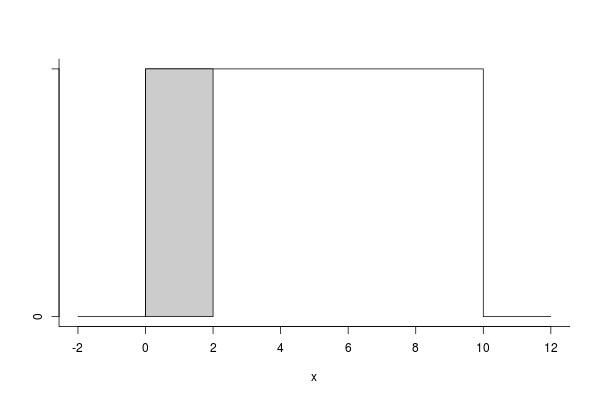
\includegraphics[width=.6\linewidth]{plots/uniformDensity0-10.png}

% x <- c(-2,-0.0001,0,10,10.0001,12)
% plot(x, dunif(x,0,10),  ylab = "", yaxt = "n", type = "l")
% rect(0,0,2,.1, col = grey(.8))
% axis(side=2, at = 0:1/10, labels = c(0,""))
% dev.copy(png, file = "plots/uniformDensity0-10.png",height=400,width = 600);dev.off(

If the area under the whole curve is 1, what is the area of the shaded rectangle?\\

In the plot below is another probability curve. What area is shaded?\\
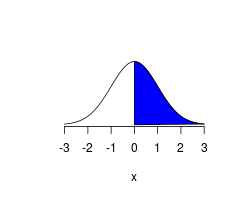
\includegraphics[width=.4\linewidth]{../plots/halfNormal.png}\vspace{-.5in}


\begin{center}
  {\large\bf Important Points}
\end{center}

\begin{itemize}
\item Curves are often used to represent probability
  distributions. The area under the whole curve must be one.
\item The connection between the dots we've been using and the curve
  is to imagine that we sample from the distribution a huge
  number of times. The dots we have been plotting would then have to
  each take up a very tiny space (like a dust mote), and instead of
  counting dots, we could just measure their area.
\item The total area under a probability density curve is one.
\item The probability of drawing a number from some interval is the
  area above the interval and under the curve.  Typically we are
  computing p-values, so we want the area under the curve more extreme
  than some t or z statistic.
\end{itemize}
   %%  pages 173 - 174  buff
  \newpage

\fancyhead[LE,RO]{
   {\it Notes }\\
   {\it Unit \unitNum\   \ Page \thepage }
}
%Intentionally left blank
\phantom{No text here}
\newpage


\fancyhead[LE,RO]{
   {\it \theTopic }\\
   {\it Unit \unitNum\  Activity \dayNum \ Page \thepage }
}
 \def\theTopic{Normal and t Distributions }
\def\dayNum{21 }

\section{ Theoretical Distributions}


  Whatever your field of study, you will need to read  research
  articles which present statistical inference like p-values and or
  confidence intervals.  We hope you now understand how those are
  properly used. In particular:
  \begin{itemize}
  \item Always report p-values. Smaller p-values provide stronger
    evidence against the null hypothesis.
  \item Confidence intervals are a list of ``plausible'' values.
    Our confidence is in the process used to build intervals, not
    in one interval. 
  \end{itemize}

  Many reports you read will refer to tests based on normal
  distributions rather than randomization and simulation.
  Before we had modern computers and the web apps we've been using,
  people had to use tables to look up probabilities to make confidence
  intervals and compute p-values.  We'll now look into these methods
  as a ``short cut'' alternative to simulations.
 % You've learned to use StatKey, and that's a useful skill because
 % it's freely available and you can actually use it to analyze real
 % data in the future.  However, if 
  We encourage you to take more statistics, for example regression 
  is a powerful technique used to describe relationships between
  quantitative variables.    We are happy to visit with you
  about possibilities for more statistics (Stat 217 is a great second
  course).  Part of the motivation for this lesson (and Unit 3 in
  general)  is to make it easier to
  continue your statistical adventures.

 
\subsection{  Shapes of Data Distributions}

  Look at these three different data sets. Each histogram is overlaid
  with a ``curve''. \\
\hspace*{2.6cm}A  \hspace*{5cm}B  \hspace*{4.5cm}C \\
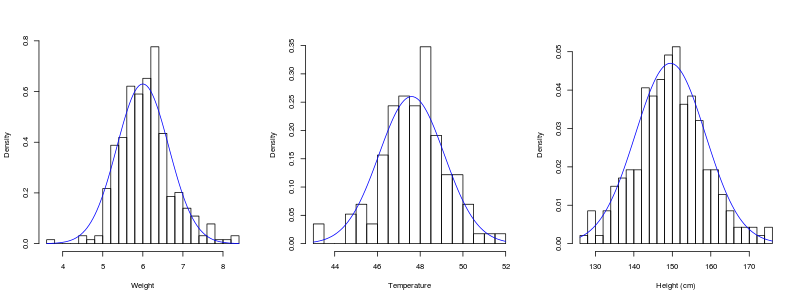
\includegraphics[width=.9\linewidth]{../plots/normals.png}

A) Weights (g) of newly born lab rat pups. 
B) Mean annual temperatures ($^\circ F$) in Ann Arbor, Michigan.
C) Heights (cm) of 14 year old boys in Oxford, England. \vspace{-.1in}


\begin{enumerate}
  \item  In what ways are the three distributions similar and different?
\begin{students}
        \vspace{3cm}        
\end{students}

\begin{key}
{\it Means and spreads all differ, but the shapes are quite
  similar -- sort of bell-shaped. }
\end{key}

  Many distributions we look at have a shape similar to those above.
  Most of the data lies close to the mean, and the left and right
  sides are symmetric.  We call it ``bell-shaped'' and the best example is
  called the ``Normal'' distribution.
\end{enumerate}

{\bf Important fact:}\\
{\sf Statistics vary from sample to sample, and the pattern is
  predictable.  For many statistics, the pattern of the sampling
  distribution resembles a normal distribution with a bell-shaped
  curve. } \\
  Studying the normal distribution will allow us to find
  probabilities for statistical inference which do not require running
  simulations.

 {\bf Normal Distributions all have the same shape.\\
They differ only in mean ($\mu$) and spread ($\sigma$).}  We write $X
\sim N(\mu, \sigma)$ to say that random variable $X$ is normally
distributed with center $\mu$ and spread (officially: standard
deviation) $\sigma$.  This distribution
has two {\bf parameters}, $\mu$ and $\sigma$. 

{\bf Definition:  Random Variable} is a number which comes from some
random process, like randomly selecting one unit from a population and
measuring it.

The  {\bf Standard Normal Distribution} has center $\mu=0$ and spread
$\sigma = 1$.  We can ``standardize'' any normal distribution to make
it have center 0 and $\sigma = 1$ by subtracting $\mu$ and dividing by
$\sigma$. If a random measurement, $X$, has a N$(\mu, \sigma)$
distribution, then $$Z = \frac{X - \mu}\sigma$$ has a N(0,1) distribution. 
We use the standardized versions to say how many standard deviations
($\sigma$'s) an observation is from the mean ($\mu$). 


\begin{enumerate}
\setcounter{enumi}{1}
  \item  When you get back results from standardized tests, they give
    a score and tell you your ``percentile rank'', the percentage
    of test takers who score at your level or below.  The exam scores have
    an approximately normal distribution.  For example, with ACT, $\mu
    = 21$ and $\sigma = 5$. In most cases we don't know these
    parameters, but for standardized tests they are known.
    \begin{enumerate}
    \item What is the standardized $z = (x-\mu)/\sigma$ score for
      Amber who got 27 on the ACT? 
\begin{students}
        \vspace{2cm}        
\end{students}
\begin{key}
  $$ \frac{25 - 21}{5} = 1.20$$
\end{key}
    \item What is Amber's percentile rank?  Select
      \fbox{Normal Distribution} under \fbox{One Categ.} on the 
      \webAppURLFrst\ 
      app and plug her {\bf standardized score}  into
      the first line of this web app.  Explain what
      the number means in terms of other  test takers.  
\begin{students}
        \vspace{1cm}        
\end{students}

\begin{key}
 {\it .885 or 88.5\% of students taking the ACT are at this level or lower.}
\end{key}
   \item Bert took the SAT instead of the ACT, and
      SAT scores are normally distributed with mean $\mu = 1500$
     and spread $\sigma = 300$. Bert's score was  1720. What is Bert's
     standardized score?
\begin{students}
        \vspace{2cm}        
\end{students}
\begin{key}
  $$ z = \frac{1720 - 1500}{300} = 0.733$$
\end{key}
    \item What is Bert's percentile rank? Compare how well he did on
      the SAT with how well Amber did on the ACT. 
\begin{students}
        \vspace{2cm}        
\end{students}

\begin{key}
 {\it .768 or 76.8\% of students taking the SAT are at this level
    or lower.  Amber did better relative to others taking the ACT than
    Bert did relative to SAT takers.}
\end{key} 
  \end{enumerate}
\end{enumerate}

{\bf Definition:  Probability}: the proportion of times -- in the long run
-- that a particular outcome occurs.  For example, the probability of
drawing a ``heart'' from a well-shuffled deck of cards is
0.25. Probabilities must be between 0 and 1. 


\begin{minipage}{.80\linewidth}
{\bf Normal Probabilities} are areas under the normal curve.  Area
under the  {\bf entire} curve is 1.   What area is shaded for this normal
distribution? \vspace*{2cm}
\end{minipage}
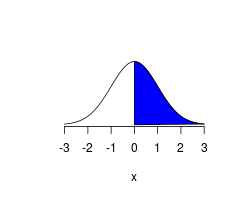
\includegraphics[width=.2\linewidth]{../plots/halfNormal.png}
\vspace{-1.9cm}

We can also go from a percent to a percentile (or, from a probability
between 0 and 1 to a {\bf quantile}) by back--solving the ``Z'' formula for
$X$ like this:  
$$\mbox{Start with } Z = \frac{X-\mu}{\sigma}  \mbox{ and solve for
  $X$ to get }
  X = Z\sigma + \mu $$

What SAT score is needed to be in the top 10\% of SAT takers?\\
In the same web app, put 0.10 in the second box and click upper (or 0.90
and click lower). That returns a $Z$ value of 1.282, so 
$ X = 1.282 \times 300 + 1500 = 1884.5$.  SAT  scores are always
multiples of ten, so a score of 1890 puts a person into the top 10\%,
or above the 90$^{th}$ percentile. 

\begin{enumerate}
\setcounter{enumi}{2}
\item {\bf Your Turn:} Suppose birth weights of full term babies have
  a $N(3000, 700)$ (in grams) distribution. Show your work, that is,
  how you standardize each value, or ``unstandardize'' to get a
  percentile.
\begin{enumerate}
\item 
  How heavy is a baby whose weight is at the  98$^{th}$
  percentile? The 5$^{th}$ percentile? 
\begin{students}
        \vspace{1cm}        
\end{students}

\begin{key}
{\it Standardized percentiles are 2.054 and -1.645.  Converting to
    birth 
    weights( times 700 + 3000): 4438g and 1848.6g. }
\end{key}

\item What is the probability that a randomly chosen baby will weigh
  under 3500g?  Under 2500g?
\begin{students}
        \vspace{1cm}        
\end{students}

\begin{key}
 {\it $Z = \pm 500/700 = \pm 0.714$, Probabilities: 0.762, 0.237}
\end{key}
\item What proportion of birth weights are within one standard deviation of the  mean? Within 2 SD's? within 3 SD's?
\begin{students}
        \vspace{.5cm}        
\end{students}

\begin{key}
 {\it 0.683, 0.955, 0.997 }
\end{key}

  \end{enumerate}
\end{enumerate}

Note: This is called {\bf the empirical rule}.  The probability of being within
2 SD's is often rounded to 95\%.
\begin{students}

\end{students}

\subsection{ t Distributions}


To standardize a normal distribution,  we need to know its true mean,
$\mu$, true standard deviation, $\sigma$. Problem: we seldom know the
true parameter values.  We can work around the unknown
mean pretty easily, but not knowing $\sigma$ causes a bit of a problem.

{\bf Discuss}: Look back to Activity 2 -- estimates of spread. What
can we plug in to estimate the unknown population spread, $\sigma$? 
\begin{students}
        \vspace{2cm}        
\end{students}

\begin{key}
 {\it $s$, the spread in the sample}
\end{key}

In the early 1900's, Mr.~Gossett was working for Guinness Brewery.  He
discovered that using an estimated instead of ``known'' $\sigma$
changes the distribution from regular normal to something called a
$t$-distribution which is more spread out.  Furthermore, there is not
just one $t$-distribution, but many. You have to pick the right t
distribution based on your sample size.

This make sense because as sample size gets big, $s$ becomes a better
and better estimate of $\sigma$.  Here is a picture of several
t-distributions compared to a standard normal distribution.  

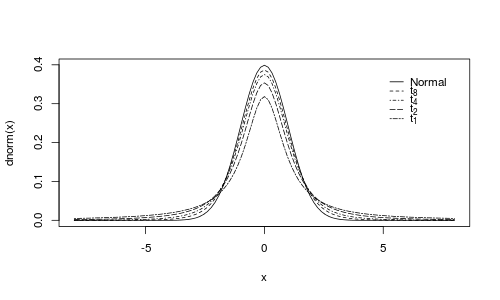
\includegraphics[width=.7\linewidth]{../plots/t-normalDensities.png}
 % curve(from=-8,to=8, dnorm(x))
 % curve(from=-8,to=8, dt(x,1) , lty=6, add=TRUE)
 % curve(from=-8,to=8, dt(x,2) , lty=5, add=TRUE)
 % curve(from=-8,to=8, dt(x,4) , lty=4, add=TRUE)
 % curve(from=-8,to=8, dt(x,8) , lty=2, add=TRUE)
 % legend(5, .38, bty="n", lty=c(1,2,4,5,6), c("Normal",expression(t[8]),expression(t[4]),expression(t[2]),expression(t[1])))
 %  dev.copy(png,"plots/t-normalDensities.png",
 %  height=300,width=500);dev.off()

We can standardize like this:
$$ t = \frac{X - \xb}{s}\mbox{\ \  or go the other way:\ \ } x = \xb
+ t \times s$$
and use the same web app to compute the 
probabilities and quantiles for $t$-distributions just as we did with normal
distributions. The one additional fact needed is that for a one-sample
mean, we use $n-1$ (sample size minus 1) as the {\bf``degrees of
  freedom''} which define the t distribution needed.  When you select
\fbox{t distribution} under \fbox{One Quant.} or \fbox{Two Quant}, you'll be able to set
the degrees of freedom.

Example:\\
Heights for adult men in the US are close to normally distributed.
We'll take 70 inches to be the mean height. From a simple random
sample of 20 men,  we compute a sample standard deviation of $s = 3.3$
inches.  
\begin{enumerate}
\setcounter{enumi}{5}
\item You will use a t-distribution with what degrees of freedom?
\begin{students}
        \vspace{1cm}        
\end{students}

\begin{key}
 {\it 19}
\end{key}

\item Use the appropriate $t$ distribution to determine how unusual it
  is to see a man who is over 76 inches tall. Show your standardized
  value and the probability.
\begin{students}
        \vspace{1cm}        
\end{students}

\begin{key}
 {\it t = 1.818, $P(t_{19} > 2) = 0.042$ }
\end{key}

\item Under 68 inches tall?
\begin{students}
        \vspace{1cm}        
\end{students}

\begin{key}
{\it  t = -1.212, $P(t_{19} < -1.212) = 0.12$ }
\end{key}

\item Between 65 inches and 75 inches? (You have to enter each
  standardized value, selecting ``Lower'', and subtract to get the
  area in between.)
\begin{students}
        \vspace{1cm}        
\end{students}

\begin{key}
 {\it $t$ values are 1.515 and -1.515. subtract 0.073 from 0.927,
    or use the \fbox{Center} choice to get 0.854. }
\end{key}

\end{enumerate}


\begin{center}
  {\large\bf Take Home Message}
\end{center}
 
\begin{itemize}
\item Theoretical distributions are a shortcut method to obtain
  probabilities for p-values and confidence intervals.
\item Normal and t distribution probabilities are areas under a
  curve. We can get them from statistical computing packages.
\item Both normal and t distributions are symmetric and
  bell--shaped. The t-distributions are more spread out because we
  have to estimate the standard deviation.
\item When $\sigma$ is known use a normal distribution. Otherwise, use
  a t-distribution with $n-1$ degrees of freedom for just one
  sample. (This changes for 2 or more samples).
\item To look up normal or t probabilities, we have to standardize by
  subtracting $\mu$ and dividing by $\sigma$ (for normal) or $s$ (for
  t). The standardized score tells us how many standard deviations we
  are from the center.
\item You need to be able to go either way: find a probability from a
  Z or t score, or find the percentile from the
  probability.

\item Empirical Rule for data with a normal distribution:
  \begin{itemize}
  \item 68\% of the values fall within one SD of the mean.
  \item 95\% of the values fall within 2 SD of the mean, and 
  \item 99.7\% of the data fall within 3 SD of the mean.
  \end{itemize}
This does not work with t distributions unless you have really large
degrees of freedom.
\item Use this space for questions or your own summary.\vfill
\end{itemize}




%% 5 pages.  Add CLT or LLN?

 % x<- c(0,seq(0,3,.01))
 % y<- c(0,dnorm(x[-1]))
 % curve(dnorm(x), from = -3, 3, yaxt="n", ylab="", bty="n")
 % polygon(x,y,col="blue")
 % dev.copy(png,file="halfNormal.png", height=200,width=240);dev.off()

%% 5 pages.  Add CLT or LLN?



\begin{center}
  {\large\bf Assignment}
\end{center}

\begin{itemize}
%\item D2Quiz 9 is due Monday, April 4.  Fill it in on D2L.
%\item D2Box 9 is due Thursday, April 7. Turn it in as a pdf in th D2L Dropbox.
 %%  We strongly encourage you to get help in the Math Learning Center.
\item Watch the ``Normal Distributions'' and ``t Distributions''
  videos, \# 1 and 2 under Unit 3.
\item Read the next two pages before your next class.
\end{itemize}

  %%  pgs 175-182

\fancyhead[LE,RO]{
   {\it Notes }\\
   {\it Unit \unitNum\   \ Page \thepage }
}
%Intentionally left blank
\phantom{No text here}
\newpage

 \newpage
\fancyhead[LE,RO]{
   {\it \theTopic }\\
   {\it Unit \unitNum\   \ Page \thepage }
}
  \def\theTopic{Reading 18}


\section{ Data Distribution versus Sampling Distribution }



For the SAT,  ACT, and baby weight examples, we assumed that the
individual data points have a normal distribution.   We said that the
score of one individual test taker or the weight of one baby follows a
normal distribution.  Think of picking one value at random from one of
these distributions:



% par(mfrow=c(1,3))
% curve(dnorm(x, 21,5), 6, 36, xlab = "ACT", bty="l", yaxt="n", ylab = " ")
% curve(dnorm(x, 1500,300), 400, 2400, xlab = "SAT", bty="l", yaxt="n", ylab = " ")
% curve(dnorm(x, 3000,700), 900, 5100, xlab = "Baby Weights", bty="l", yaxt="n", ylab = " ")
% dev.copy(png, "plots/3normals.png", height = 200, width = 600);dev.off()

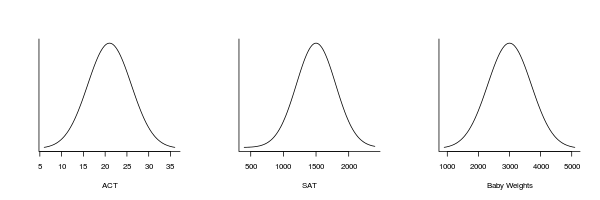
\includegraphics[width=\linewidth]{plots/3normals.png}

Values near the centers of the curves are more likely to get picked
than values out in the tails. 



Another important use of distributions is the {\bf sampling
  distribution} of a {\bf statistic}.  We have already been using sampling
distributions, but have simulated draws to get them and have drawn
them as dot plots.  We'll see in the next lesson that the sampling
distribution of a proportion often is well approximated by a normal
distribution. Before we get there, though, we want to insert a
reminder about just what a sampling distribution is.

The {\bf sampling distribution} of a {\bf statistic} is a description
of all the possible values that statistic can take and the probability
of each.  For example, if we randomly sample weights of 9 full term
babies, each coming from N(3000,700), the sample mean will also be
normally distributed with mean 3000, but the standard deviation will
be 233g instead of 700g.  Think about the sampling distribution this
way: 
\begin{itemize}
\item When we randomly sample and compute a statistic from the sample,
  we don't know what we'll get ahead of time for any one draw, and
  won't know what mean we will get.  The mean ($\xb$) is, then, a random
  variable.
\item We do know quite a bit about the distribution of $\xb$. Because
  the distribution of the individual data points is normal, so is the
  distribution of $\xb$. \\
  Averaging values together does not change the
  center, so the center of the distribution of $\xb$ is also 3000g.  \\
  Averaging pulls in extremes, and the spread of the sampling
  distribution becomes $700/\sqrt{9} = 233.3$g.
\end{itemize}\vspace{1in}



\begin{center}
  {\large\bf Important Points}
\end{center}

\begin{itemize}
\item  It is important to distiguish between the sampling distribution
  of a statistic and the underlying distribution of individual data
  points.  
\item If we start with a normal distribution for individual points,
  then the sample mean will also have a normal distribution with the
  same center.
\item As sample size increases, spread decreases: the standard
  deviation of $\xb$ is  $\frac{\sigma}{\sqrt{n}}$. 
\end{itemize}

   %%  pages 183 - 184 buff
%  \newpage
%  \ \ \ \thispagestyle{empty}
 \newpage 

\fancyhead[LE,RO]{
   {\it \theTopic }\\
   {\it Unit \unitNum\  Activity \dayNum \ Page \thepage }
}

\def\theTopic{Normal Proportions }
\def\dayNum{22 }


\section{  Proportions and the Normal Distribution}


If we mix 40 blue balls and 80 gold balls together in a jar and draw
out 30 at random with replacement, the sampling distribution for the
proportion of blue balls in a sample of size 30 looks like this:

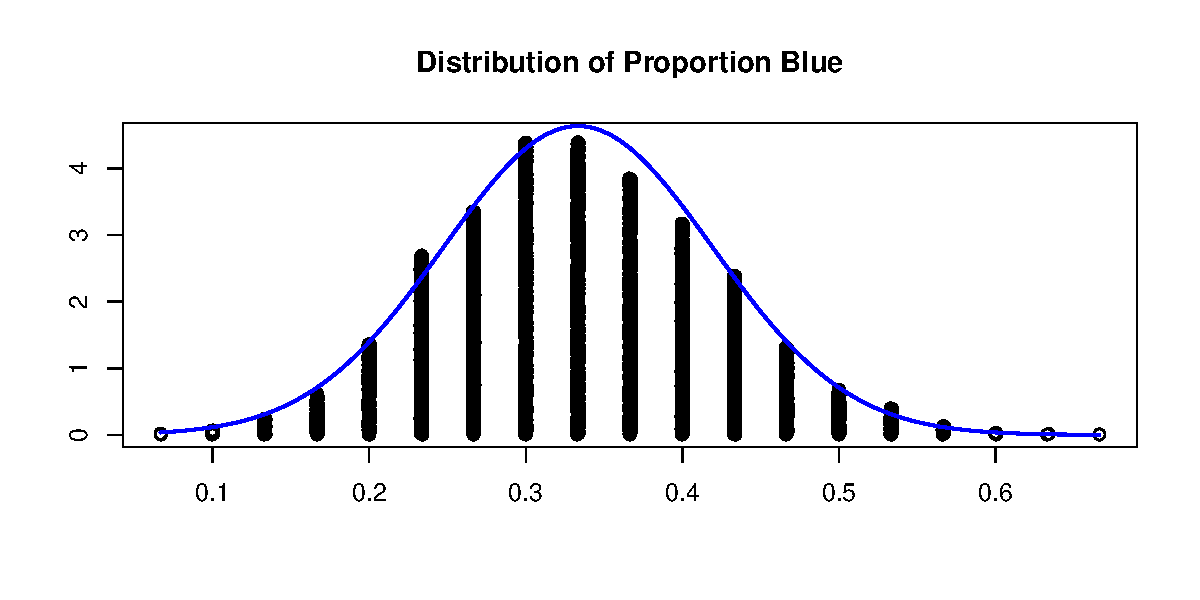
\includegraphics[width=.8\linewidth]{../plots/sample1.pdf}

Each of 5000 dots came from a computer simulation in which we sampled
30 draws from the container at random with replacement, and computed
the proportion of blue balls in the simulated sample.  The density
curve shown on top of the dots is the density of the normal
distribution with the same center and spread as the distribution of
dots.

With modern computers, we can easily simulate random draws five or ten
thousand times, and/or we can easily obtain probabilities from the
normal distribution.  Both are valid tools, and each method can give
us the p-values and confidence intervals that we need.  We did the
simulation approach first because it allowed us to bypass two weeks of
more theoretical probability and quickly get to the meat of this
course -- statistical inference.  Now it's time to see how the other
approach works, and we'll continue to emphasize the interpretation of
p-values and confidence intervals.  


%% <<sample1, echo=FALSE, fig.width=6,fig.height=4,out.width='.75\\linewidth'>>=
%%   reps <- 5000
%%   n <- 30
%%   p <- 1/3
%%   blueProp <- rbinom(reps,n,p) / n
%%   x <- sort(blueProp)
%%   y <- unlist(tapply(x, x, function(z) 1:length(z))) /reps / diff(range(x)) * (length(unique(x))-1.5)
%% ##  rescale to meet normal density
%%   plot(jitter(x, .1), y, main = "Distribution of Proportion Blue", xlab = "", ylab = "")
%%   curve(dnorm(x,p,sqrt(p*(1-p)/n)),add=TRUE,col=4,lwd=2)
 %  dev.copy2pdf(file="plots/sample1.pdf",height=4,width=8)

% # summary(nlme::RatPupWeight$weight)
% #   Min. 1st Qu.  Median    Mean 3rd Qu.    Max. 
% #  3.680   5.650   6.055   6.081   6.398   8.330 
% # sd(nlme::RatPupWeight$weight)
% #[1] 0.6474272
% # locator(1) #$y 0.6190716
 
  %# summary(faraway::aatemp$temp)
 %#   Min. 1st Qu.  Median    Mean 3rd Qu.    Max. 
 %#  43.41   46.78   47.73   47.74   48.64   51.89 
 %# sd(faraway::aatemp$temp) ] 1.526413
 %# locator(1)$y[1] 0.2773441

%# sd(nlme::Oxboys$height)
%#[1] 9.10321
 % #summary(nlme::Oxboys$height)
 % #  Min. 1st Qu.  Median    Mean 3rd Qu.    Max. 
 % # 126.2   143.8   149.5   149.5   155.5   174.8 
 % #locator(1) # 0.04889153
 %
 % par(mfrow=c(1,3))
 % hist(nlme::RatPupWeight$weight,breaks=20,probability=TRUE, main=" ",
 % xlab = "Weight")
 % curve(dnorm((x-6)/0.647)/.3989*.63,col=4,add=TRUE)
 % hist(faraway::aatemp$temp,breaks=18,probability=TRUE, main=" ", xlab
 % = "Temperature")
 % curve(dnorm((x-47.6)/1.526)/.3989*.26,col=4,add=TRUE)
 % hist(nlme::Oxboys$height,breaks=18,probability=TRUE, main=" ", xlab =
 % "Height (cm)")
 % curve(dnorm((x-149.5)/9.1)/.3989*.047,col=4,add=TRUE)
 % dev.copy(png, file="plots/normals.png",height=300,width=800);dev.off()
%% @ 
      
%% 
  
We can use spinners, card shuffles,  and coin flips to simulate the distribution
of a proportion.  From that distribution we use the standard
deviation of the resampled points to get the standard error of
$\phat$.  We added two standard errors 
to -- and subtracted two standard errors from -- the point estimate to build our
confidence interval.  In order to use the normal distribution instead of a
simulation,  we need this formula for standard error of the sample
proportion: 
    $$ SE(\widehat{p}) = \sqrt{\widehat{p}(1-\widehat{p})/n} $$
 We can then multiply $SE(\widehat{p})$ by the appropriate $z^*$
 value from the normal distribution to get whatever confidence
 level we need.  Setting margin of error to $2 SE$ was a good
 approximation for a 95\% confidence interval, but you'll see in
 this web app that a more precise value is 1.96 $SE$'s on each
 side.


{\bf Notation:} We have two ways to describe the same measure
of spread. For any distribution, we can compute the spread, or
standard deviation of the sampled values.  When we talk about the
sampling distribution of a statistic, we can  refer to the
standard deviation of the sampling distribution because it is a
distribution, so it has some ``spread''.   However, we prefer
to talk about the ``Standard Error'' (or SE) of the statistic.  We'll
be able to show the difference better when we look at the mean of a
continuous variable, so we'll come back to this. 

When we write $SE(estimate)$ as in $SE(\phat)$ or $SE(\xb)$, we {\bf
  do not} mean to multiply $SE$ by the estimate. This is notation to
say SE is a function which we apply to the estimate. We read it as
``standard error of $\ldots$'' just like when we take log of $x$ we
write $\log(x)$.  

\subsection{ Confidence Intervals}

The general form is 
$$ \mbox{estimate} \pm z^* SE(\mbox{estimate})$$
or for proportions:
$$ \widehat{p} \pm z^*\sqrt{\widehat{p}(1-\widehat{p})/n}$$

To build confidence intervals, we use the same $z^*$ values over and
over again.  Go to the web app
\webAppURLFrst , select
\fbox{Normal Distribution} under \fbox{One Categ} and  put
confidence levels 0.80, 0.90, $\ldots$, 0.99 into the probability box
(one at a time).  Change \fbox{Lower} to
\fbox{Center} to get the confidence limits. Write them into this
table.  \vspace{1cm}
 
\begin{students}
   \begin{tabular}{l|rrrrr}
    Confidence level: &  \hspace{1cm}80\% &  \hspace{1cm}90\% &  \hspace{1cm}95\% & \hspace{1cm} 98\% & \hspace{1cm} 99\% \\ \hline
    $z^*$ cutoff  &  &  & 1.96 &  & 
  \end{tabular}
\end{students}
\begin{key}
   \begin{tabular}{l|rrrrr}
    Confidence level: &  \hspace{1cm}80\% &  \hspace{1cm}90\% &  \hspace{1cm}95\% & \hspace{1cm} 98\% & \hspace{1cm} 99\% \\ \hline
    $z^*$ cutoff  &1.282  &1.645  & 1.96 &2.326& 2.575
  \end{tabular}
\end{key}


Let's try it out:  
 \begin{enumerate}
   \item 
     In a survey of  2142 American adults, 1221 gave the opinion that
     college is a ``poor to fair'' value.  We want to estimate the
     proportion of all American adults with that opinion using a 99\%
     confidence interval.  
     \begin{enumerate}
     \item Compute $\widehat{p}$ for these data. 
\begin{students}
        \vspace{1cm}        
\end{students}

\begin{key}
  {\it 0.57 }
\end{key}
     \item \label{propSE} Compute the standard error of the estimate.
\begin{students}
        \vspace{1cm}        
\end{students}

\begin{key}
  {\it $ \sqrt{0.57\times 0.43/2142} = 0.0107$ }
\end{key}

     \item Find the margin of error and compute a 99\% CI using the
       multiplier you found   above.
\begin{students}
        \vspace{1cm}        
\end{students}

\begin{key}
  {\it ME = $ 2.575 \times 0.0107 = 0.02755$, CI: $0.57 \pm  0.0276 = (0.542, 0.598 )$ }
\end{key}

     \item If we use resampling to create a 99\% bootstrap percentile
       confidence interval, it is $(0.542, 0.597)$ and the {\sf SE} in
       the plot is 0.011.  Which interval is narrower? 
\begin{students}
        \vspace{1cm}        
\end{students}

\begin{key}
  {\it Bootstrap is a hair narrower.}
\end{key}

     How similar is the standard error from \ref{propSE} to the
     bootstrap SE?        
\begin{students}
        \vspace{2cm}         
\end{students}

\begin{key}
  {\it Very close. Off just by round off error?}
\end{key}

\item Interpret the interval in the context of this problem.  What do
  we mean by the word ``confidence''?    
\begin{students}
        \vspace{3cm}        
\end{students}

\begin{key}
  {\it We are 99\% confident that the true proportion of US adults
  who thought that college was a poor to fair investment is within the
interval (0.542, 0.597). Our confidence is in the process: when we use
this method over and over take a sample and compute a 99\% CI from it,
in the long run, 99\% of those intervals will contain the true parameter.}
\end{key}
     \end{enumerate}
   \end{enumerate}
 

\subsection{ Assumptions}


  To do any statistical analysis, we must make some assumptions.  We
  should always check to see if the data indicate a violation of an
  assumption. For the methods used before today we need:
     \begin{itemize}
     % \item A population of size at least $10n$. 
     %   (If a sample is a really large part of the population, our
     %   methods over-estimate sampling variation.) 
     \item Representative sample. 
     \item Independent trials (one outcome has no effect on another).  
     \end{itemize}
   
  Using normal distributions adds another assumption:
   \begin{itemize}
     \item Large enough sample size to expect at least 10
       successes   and  at least 10  failures.  If you are building a
       confidence interval, just make sure the counts are over 10. If
       you are conducting a hypothesis test, we need $np_0\geq 10$ and
       $n(1-p_0) \geq 10$. 
     \end{itemize}\vspace{1cm}


   \begin{enumerate}
     \setcounter{enumi}{1}
   \item We'll check the assumptions for the survey in \#1.  Assume
     these adults were selected via random phone number dialing.
     \begin{enumerate}
%         \item Is population size at least $10n$ ($n = 2142$)? 
% \begin{students}
%         \vspace{.7cm}        
% \end{students}
% \begin{key}
%   {\it  Yes, there are more than 22,000 US adults. }
% \end{key}
        \item Representative sample?   
\begin{students}
        \vspace{.7cm}        
\end{students}

\begin{key}
  {\it Yes, the participants were randomly selected.}
\end{key}
        \item Independent trials?   
\begin{students}
        \vspace{.7cm}        
\end{students}

\begin{key}
  {\it Yes, by random selection.}
\end{key}
        \item At least 10 successes? at least 10 failures?   
\begin{students}
        \vspace{.7cm}        
\end{students}

\begin{key}
  {\it  Yes, 1221 successes and $2142-1221 = 921$ failures.}
\end{key}
\end{enumerate}

\item In an earlier assignment  you checked to see if a roulette wheel was
     fair.  Were these assumptions met? The
     observer saw 3 ``Greens'' in 30 spins, and the  chance of
     green for a fair wheel is $2/38$. 
     \begin{enumerate}
%         \item Is population size at least $10n$ ($n = 30$)? 
%           Hint: How many spins are possible?    
% \begin{students}
%         \vspace{.7cm}        
% \end{students}
% \begin{key}
%   {\it  An almost infinite number, so assumption is met.}
% \end{key}
        \item Representative sample?   
\begin{students}
        \vspace{.7cm}        
\end{students}

\begin{key}
  {\it  One spin should be like another, so I don't question this  assumption.}
\end{key}
        \item Independent trials?   
\begin{students}
        \vspace{.7cm}        
\end{students}

\begin{key}
  {\it  If there is no cheating, this assumption is met.}
\end{key}
        \item At least 10 successes? at least 10 failures?   
\begin{students}
        \vspace{.7cm}        
\end{students}

\begin{key}
  {\it  Not met. 27 ``Failures'' and only 3 ``Successes''.}
\end{key}
     \end{enumerate}


    \item In the Unit 1 Review you estimated the probability
      a kissing couple leans to the right from data in which 80 of 124
      couples did lean to the right. Let's check assumptions. 
  
     \begin{itemize}
%         \item Is population size at least $10n$ ($n = 124$)? 
% \begin{students}
%         \vspace{.7cm}        
% \end{students}

% \begin{key}
%   {\it  All couples, so assumption is met.}
% \end{key}
        \item Representative sample?   
\begin{students}
        \vspace{1cm}        
\end{students}

\begin{key}
  {\it  Sort of random observations, so I hope this   assumption is met.}
\end{key}
        \item Independent trials?   
\begin{students}
        \vspace{1cm}        
\end{students}

\begin{key}
  {\it  Couple should act independently, so this assumption is met.}
\end{key}
        \item At least 10 successes? at least 10 failures?   
\begin{students}
        \vspace{1cm}        
\end{students}

\begin{key}
  {\it  Yes, $80>10$ and $44 > 10$}
\end{key}
     \end{itemize}
     \begin{enumerate}
     \item Now we'll build a 99\% confidence interval for the true
       proportion of couples leaning right when kissing using normal
       procedures. 
       \begin{enumerate}
       \item What is the sample statistic?  
\begin{students}
        \vspace{1cm}        
\end{students}

\begin{key}
  {\it  0.645}
\end{key}
       \item What is the standard error of $\widehat{p}$ for these
         data?   
\begin{students}
        \vspace{.7cm}        
\end{students}

\begin{key}
  {\it  $\sqrt{0.645 * 0.355 / 124} = 0.0430 $}
\end{key}
       \item From the table about two pages back, what $z^*$ values
         goes with 99\% confidence?   
       \end{enumerate}
\begin{students}
        \vspace{.7cm}        
\end{students}

\begin{key}
  {\it  2.576}
\end{key}
       \item Build the interval and interpret its meaning. 
\begin{students}
        \vspace{2in}
\end{students}

\begin{key}
 {\it $(0.534, 0.756)$.  We are 99\% confident that the true
    proportion of couples who lean right when kissing is between 53.4
    and 75.6\%. }
\end{key}
     \end{enumerate}
   \end{enumerate}

\subsection{   Hypothesis testing }

 Reminder:  when we do hypothesis testing, we give the benefit
 of the doubt to: \underline{\hspace{1in}}.

 Our assumption of ``innocent until proven guilty'' changes the
 formula for standard error.  We plug in the null hypothesis value
 instead of the sample proportion, so when hypothesis testing: $
 SE(\widehat{p}) = \sqrt{p_0(1-p_0)/n}$. Secondly, instead of counting
 points as or more extreme than the observed statistic, we will use
 the normal distribution to compute the probabilities.  To do that, we
 need to convert the distance between $p_0$ and $\widehat{p}$ to ``standard
 deviation'' units by dividing by $SE(\widehat{p})$.  The complete
 formula is:
  $$ z = \frac{\widehat{p} - p_0}{SE(\widehat{p})} = 
         \frac{\widehat{p} - p_0}{\sqrt{p_0(1-p_0)/n}}$$
   
 We will illustrate with the ``Kissing on the Right'' data. As we did
 before, we will not assume which direction the alternative will
 take, but the null is that couples are equally likely to lean
 left or right. 
 
    \begin{enumerate}
\setcounter{enumi}{3}
    \item State null and alternative hypotheses in symbols and
      words.\\
      $H_0:$ 
\begin{students}
    \vspace{1.2cm}    \\
\end{students}
\begin{key} 
{\it $p = .5$.  Half of all couples lean right when kissing.}
\end{key}
$H_a:$
\begin{students}
    \vspace{.7cm}    \\
\end{students}

\begin{key} 
{\it $p \neq .5$.  The true proportion of couples leaning right when
  kissing is not one half.}
\end{key}
\item Compute the $SE(\widehat{p})$ using the null hypothesis value
  for $p$. 
\begin{students}
    \vspace{1cm}    \\
\end{students}

\begin{key} 
{\it $SE(\widehat{p}) = \sqrt{.5(.5)/124} = 0.0449$}
\end{key}

  \item Build the $z$ statistic by dividing the difference between
    $\widehat{p}$ and $p_0$ by $SE(\widehat{p})$. 
\begin{students}
    \vspace{1cm}    \\
\end{students}

\begin{key} 
{\it $z = \frac{.645 - .5}{0.0499} = 3.23$}
\end{key}

  \item Put the standardized $z$ value into the web app 
    \webAppURLFrst \ 
    \fbox{One Categ} -- \fbox{Normal Distribution} and ask for
    the \fbox{Extremes}.  What part of the plot is shaded?  What is
    the (total) p-value and how strong is this evidence against $H_0$?  
\begin{students}
    \vspace{1cm}    \\
\end{students}

\begin{key} 
{\it $2 \times .001 = .002$  This is  very strong evidence against the
  null. }
\end{key}


\item Report the strength of evidence.  At the $\alpha = .01$ level of
  significance, what do you decide to do with $H_0$?  What is your
  conclusion?
\begin{students}
 \vspace{3cm}
\end{students}

\begin{key} 
{\it We  reject $H_0$
  at the 1\% significance level.  We conclude that the true proportion of
  couples who lean right when kissing is over 0.50.}
\end{key}

\end{enumerate}

\begin{center}
  {\large \bf Rock, Paper, Scissors}
\end{center}

A student played a game of ``Rock, Paper, Scissors'' with each of 120
inexperienced players and found that 55 of his opponents first chose
``Rock''.  We want to test to see if the three options are equally
likely and to build a confidence interval for the true proportion to
pick ``Rock''.

\begin{enumerate}
 \setcounter{enumi}{8}
 \item  Check the assumptions.
\begin{students}
\\   \vspace{2cm}    
\end{students}

\begin{key} 
 {\it % There is a huge population of potential first time players, so
  % we have less than 10\% of the population.  
   We'd like to know how the
  opponents were selected. We can't assume they are representative,
  and if they watched some of his earlier games, they might be
  influenced in their 
  choices. We cannot assume independence from the data provided. We do
have large enough sample size to use normality because $55 > 10$ and
$120-55 = 65>0$ (for CI) and $np_0 = 120\times 1/3 = 40>10$ (for
hypothesis test).}
\end{key}
\item Although you should have identified some possible problems with
  the assumptions, we will go ahead with the normal theory based
  inference. Compute $\widehat{p}$ and its SE for a confidence
  interval.
\begin{students}
    \vspace{1cm}    \\
\end{students}

\begin{key} 
{\it $\widehat{p} = 55/120 = 0.458$ with SE = $\sqrt{.458(.542)/120} =
  0.0455$}
\end{key}
\item Build a 90\% confidence interval for the true mean proportion of
  first time players who pick ``Rock''.
\begin{students}
    \vspace{1cm}    \\
\end{students}

\begin{key} 
{\it $0.458 \pm 1.645 \times 0.0455 = (0.383, 0.533)$}
\end{key}
\item Now switch to thinking of a hypothesis test using ``random
  guessing'' as the null model.  What are the null and alternative
  hypotheses? 
\begin{students}
    \vspace{2cm}    \\
\end{students}

\begin{key} 
{\it $H_0: p = 1/3$, versus $H_a:  p \neq 1/3$}
\end{key}
 
\item Compute the SE under $H_0$ and the test statistic.
\begin{students}
    \vspace{1cm}    \\
\end{students}

\begin{key} 
{\it $SE = \sqrt{1/3 \times 2/3 \times 1/120} =0.0430$, $z = \frac{0.455 - 0.333}{0.043} = 2.84$}
\end{key}


\item What is the strength of evidence (from the web app) against   $H_0$?  
\begin{students}
       \vspace{3.5cm}
\end{students}

\begin{key} 
{\it Very strong.  The p-value is $2 \times 0.002$. }
\end{key}

\item Write a short report on the hypothesis test. Include the 5 main
  points:\\
  Type of test, null hypothesis, observed result, strength of
  evidence, and scope of inference. 
  \begin{enumerate}
  \item First write it up assuming that no subject could see what anyother
subject  chose.\vfill
\item Now assume that players got to watch others and could keep track of
what others chose. What would change in the writeup (go back to our assumptions).\vspace{1in}
 \end{enumerate}


\end{enumerate}



\begin{center}
  {\large\bf Take Home Message}
\end{center}
 
\begin{itemize}
\item To use any statistical method, our assumptions must be met. We
  need representative samples and independent trials.%, and a sample size
  %less than one tenth of the population size.  
  To use the normal
  probabilities we also need at least ten successes and ten failures
  (for a CI) or $np_0 \geq 10$ and $n(1-p_0) \geq 10$.  
\item The only change to our writeups is that we describe the test as
  a ``z'' test instead of a permutation test, and the confidence
  interval is also ``z based''.
\item Write your questions and summary here.

\end{itemize}\vspace*{1in}



%% 6 pages

\begin{center}
  {\large\bf Assignment}
\end{center}

\begin{itemize}
\item Fill in the bottom 3 boxes in column 1 of the Review Table. 
\item D2Quiz 10 is due Monday Nov 14.  Take it on D2L.
\item D2Box 10 is due Thursday Nov 17. 
%%  We strongly encourage you to get help in the Math Learning Center.
%\item Watch  videos 10 and 11 under Unit 3 Examples.
\item Watch videos assigned on D2L.
\item Read the next two pages about comparing two proportions before your next class.
\end{itemize}
  %%  pgs 185-192
 \newpage 
%
\fancyhead[LE,RO]{
   {\it Notes }\\
   {\it Unit \unitNum\   \ Page \thepage }
}
%Intentionally left blank
\phantom{No text here}
\newpage


\fancyhead[LE,RO]{
   {\it \theTopic }\\
   {\it Unit \unitNum\   \ Page \thepage } 
}
 \def\theTopic{Reading 19}

\section{ Smell of Baking Bread}


\begin{center}
\vspace*{.1in}
{\bf {\large Are we better people in a pleasant environment?}}
\end{center}
\vspace{-.1in}

A study from the {\it Journal of Social Psychology}\footnote{ Nicolas Gu\'eguen, 2012.  The Sweet Smell of \ldots Implicit Helping:
 Effects of Pleasant Ambient Fragrance on Spontaneous Help in Shopping
 Malls .  {\it Journal of Social Psychology} {\bf152}:4, 397-400 }
 reports on a study of
people's behavior under two different conditions. The researchers gave
this description of their methods: 
   \quotation{ \small
``The participants were 200 men and 200 women (between the ages of
approximately 20 and 50) chosen at random while they were walking in a
large shopping mall. The participant was tested while walking near
areas containing pleasant ambient odors (e.g.: bakeries, pastries) or
not (e.g. clothing stores). Four young women (M = 20.3 years) and
four young men (M = 21.3 years) served as confederates in this
study. They were dressed in clothing typically worn by people of this
age (jeans/T-shirt/boat shoes). The confederate chose a participant
walking in his/her direction while standing in front of a store
apparently looking for something in his/her bag. The confederate was
carefully instructed to approach men and women walking alone,
apparently aged from 20 to 50, and to avoid children, adolescent, and
elderly people. The confederate was also instructed to avoid people
who stopped near a store. Once a participant was identified, the
confederate began walking in the same direction as the participant
about three meters ahead. The confederate held a handbag and
accidentally lost a glove. The confederate continued, apparently not
aware of his/her loss. Two observers placed approximately 50 meters
ahead noted the reaction of the passer-by, his/her gender, and
estimated, approximately, his/her age. Responses were recorded if the
subject warned the confederate within 10 seconds after losing the
object. If not, the confederate acted as if he/she was searching for
something in his/her hand-bag, looked around in surprise, and
returned to pick up the object without looking at the
participant.''\footnote{ibid}} 
  
Assume that when the confederate saw a person who fit the qualifications, a
coin was flipped. If it came up Heads, the subject was picked to be in
the study, if Tails, they were skipped.

Data summary:\\
 In the bakery group of 200 subjects, 154 people stopped the ``confederate'' to tell
 them they had dropped something.\\
 Outside the clothing store, 104 of the subjects stopped the
 ``confederate''.  
\begin{center}
  {\large\bf Important Points}
\end{center}


\begin{itemize}
\item  What question did the researchers want to answer?
\begin{students}
 \vspace{.8cm}
\end{students}

\begin{key}
{\it Does the smell of baking bread influence people to be more altruistic?}
\end{key}


\item Who were the subjects?
\begin{students}
 \vspace{.8cm}
\end{students}

\begin{key}
{\it 400 people in a mall}
\end{key}


\item Were they randomly selected?
\begin{students}
 \vspace{.8cm}
\end{students}

\begin{key}
{\it Yes, by coin flip to be in or not.}
\end{key}



\item Were treatments applied at random?
\begin{students}
 \vspace{.8cm}
\end{students}

\begin{key}
 {\it No. subjects were either by the clothing store or by the bakery.}
\end{key}

\item What two measurements do we have for each subject in the study?
  Which variable is the response?  
\begin{students}
 \vspace{.8cm}
\end{students}

\begin{key}
 {\it Bakery/clothing setting and helped/didn't help (the resposne)}
\end{key}

\item Thinking back to Unit 2, which situation (on the review table)
  are we using?
\begin{students}
 \vspace{.8cm}
\end{students}

\begin{key}
 {\it Two proportions.}
\end{key}




\end{itemize}



  %%  Baking bread  pages  193-194 buff
 
 \newpage
\fancyhead[LE,RO]{
   {\it \theTopic }\\
   {\it Unit \unitNum\  Activity \dayNum \ Page \thepage }
}
 \newpage
 \def\theTopic{Difference in Proportions - Z }
\def\dayNum{23 }


\section{Normal Inference - Difference in Proportions}



When we did a hypothesis test to see if the difference in  two true
proportions was zero,  for example when evaluating the effectiveness
of peanut protein, we shuffled cards and relabeled the two groups many
times. Now we'll use the normal distribution instead.  
  

 To make the switch from simulations to a theoretical distribution,
 we need, just as for a single proportion, a formula for the standard
 error of our statistic.  In the last activity our statistic was
 $\widehat{p}$ and our formula was $SE(\widehat{p}) =
 \sqrt{\widehat{p}(1-\widehat{p})/n}$.  To compare two groups, our 
statistic is $\widehat{p}_1 - \widehat{p}_2$ and we need a formula for
$SE(\widehat{p}_1 - \widehat{p}_2)$. As with a single proportion, the
form of this standard error depends on whether we are doing a
hypothesis test (assuming some $H_0$ is true) or building a confidence
interval.  We'll start with the hypothesis test which is typically
testing to see if the two groups have the same true proportion, that
is:  $H_0:\ p_1 = p_2$.
 \begin{itemize}
 \item If $H_0$ is true, the two groups are really the same, and we
   should combine them to get a better estimate of the overall
   proportion of successes. We'll call estimate $\widehat{p}_T$ where
   the ``T'' stands for ``{\bf total}'' or ``{\bf marginal}'' because it's
   based on totals which appear in the outer margin of a table.  We
   find it by combining all successes from both 
   groups, then dividing by the sum of the sample sizes. 
  $$\widehat{p}_T = \frac{x_1 + x_2}{n_1+n_2} = \frac{n_1\widehat{p}_1
    + n_2\widehat{p}_2}{n_1 + n_2}$$ 
  Recall:  we used the same combined estimate when simulating draws
  from $H_0$ earlier in Activity 12.
 \end{itemize}

 The {\bf hypothesis testing} formula for standard error of the
 difference in sample proportions is: 
 $$SE(\widehat{p}_1 - \widehat{p}_2) =
 \sqrt{\frac{\widehat{p}_T(1-\widehat{p}_T)}{n_1} +
   \frac{\widehat{p}_T(1-\widehat{p}_T)}{n_2}} =
  \sqrt{\widehat{p}_T(1-\widehat{p}_T)\left(\frac{1}{n_1} +
   \frac{1}{n_2}\right)}$$


\begin{center}
\vspace*{.1in}
{\bf {\large Are we better people in a pleasant environment?}}
\end{center}
\vspace{-.1in}

For class today, you read an article abstract about a study involving
the smell of baking bread.  Answer these questions about it:


 \begin{enumerate}
   \item  Was a random mechanism used to select the person studied?
     Explain. 
\begin{students}
 \vspace{1cm}\\
\end{students}
\begin{key}
\\ {\it Yes, if the coin flip was performed, it would randomly select
  about half of the people walking by. }
\end{key}
   \item  What was the “treatment” and how was it applied to a
     subject? 
\begin{students}
 \vspace{1cm}\\
\end{students}
\begin{key}
 \\{\it The ``treatment'' was the location: either near a bakery or
   near another type of store. It was ``set'', but not for each
   subject. Choice of treatment filtered out the potential subjects.
   It was not applied at random.}
\end{key}
   \item  Does this study fit the definition of an experiment, or is
     it observational? Explain. 
\begin{students}
 \vspace{1cm}\\
\end{students}
\begin{key}
 \\ {\it I'd say it's observational, since a given passerby probably
   was a possible subject for just one of the treatments, not both.}
\end{key}
   \item  Name three or more possible lurking variables. 
\begin{students}
 \vspace{1cm}\\
\end{students}
\begin{key}
 \\ {\it Reason for visiting the mall (need bread? or need
   clothing?).  Gender. Socio-economic status. Tendency to lose things.}

\end{key}
   \item  What is the scope of inference for this study? 
\begin{students}
 \vspace{1cm}\\
\end{students}
\begin{key}
 \\ {\it  We can only infer association within this sample because the
   subjects where only haphazardly selected, and treatments were not
   randomly applied.}
\end{key}

\item \label{Bake-hypotheses}What are null and alternative hypotheses
  for this study? Assume that researchers were not willing to state
  ahead of time whether a good smell makes people ``better'' or ``worse''. \\
  $H_0:$\
\begin{students}
 \vspace{1cm}\\
\end{students}
\begin{key}
 $p_1 = p_2$ \\
\end{key}
   $H_a: $
\begin{students}
     \vspace{1cm}\\
\end{students}
\begin{key}
   $ p_1 \neq p_2$ \\
\end{key}   

     Check you  answers just above with other groups at your table.
     Do we all agree about the direction of the alternative?  
\item Compute the following proportions:\\
    Bakery group:  $\widehat{p}_1 = $
\begin{students}
 \vspace{1cm}\\
\end{students}
\begin{key}
  $154/200 = 0.752$ \\
\end{key}
Clothing store: $\widehat{p}_2 = $
\begin{students}
 \vspace{1cm}\\
\end{students}
\begin{key}
  $104/200 = 0.52$ \\
\end{key}
    Overall: $\widehat{p}_T = $
\begin{students}
 \vspace{1cm}\\
\end{students}
\begin{key}
  $258/400 = 0.645$ \\
\end{key}

\item When testing one proportion, we created a $z$ statistic with
$z = \frac{\widehat{p} - p_0}{SE(\widehat{p})}$.  In general, we use
$$ z = \frac{\mbox{statistic - null value}}{SE(\mbox{statistic})}$$
Now our statistic is $\widehat{p}_1 - \widehat{p}_2$.  
\begin{itemize}
\item What value do we expect it to have if $H_0$ is true?
\begin{students}
 \vspace{1cm}\\
\end{students}
\begin{key}
  $0$ \\
\end{key}
\item What is the standard error of the statistic under $H_0$?
\begin{students}
 \vspace{1cm}\\
\end{students}

\begin{key}
  $SE(\widehat{p}_1 - \widehat{p}_2 ) = \sqrt{ 0.645\times 0.355
    (\frac{1}{200} +  \frac{1}{200})} = \sqrt{.002281} = 0.045$ 
\end{key}

\item Compute our $z$ statistic.
\begin{students}
 \vspace{1cm}\\
\end{students}
\begin{key}
 $z = \frac{ 0.752 - 0.52}{0.04776} = \frac{0.25}{0.045} = 5.1$ \\
\end{key}  
\end{itemize}
\item Use the web app to find the probability.  
How strong is the evidence against $H_0$?
\begin{students}
 \vspace{1cm}\\
\end{students}
\begin{key}
  \\ {\it p-value $ \leq 2 \times(0.00001) = 0.00002$ This is very, very
    strong evidence refuting the null hypothesis that people act just
    as helpfully in the two situations.  In fact, the people close to
    the bakery were much more helpful than those by the clothing
    store.  }
\end{key}

\item Write up the results as a statistical report on your own paper.
  (Suggestion:  finish the activity, then come back to this.) 
\begin{students}
 \vspace{1cm}
\end{students}

  \end{enumerate}

\subsection{ Confidence Interval for the Difference in True Proportions}

Next we want to get an interval estimate of the difference in true
proportions.  We'll use the same data to ask: ``How much more helpful
are people near a bakery than near a clothing store?''

Again, looking back to a single proportion we used $\widehat{p} \pm
z^*SE(\widehat{p})$ which is a special case of the general rule:
$$ \mbox{estimate} \pm \mbox{multiplier} \times SE(\mbox{estimate})$$

All we need to do is to find the $SE(\widehat{p}_1 - \widehat{p}_2)$.
We {\bf do not assume the two are equal}, so no $\widehat{p}_T$ is
needed. The formula is:
  $$ SE(\widehat{p}_1 - \widehat{p}_2) = \sqrt{ 
      \frac{\widehat{p}_1(1 - \widehat{p}_1)}{n_1} + 
      \frac{\widehat{p}_2(1 - \widehat{p}_2)}{n_2}} $$
You might ask why there is a plus sign between the two terms inside
the square root, but a minus sign in the estimator.  It's because each
sample  proportion has some variability, and $\widehat{p}_1 - \widehat{p}_2 $ 
can vary due to changes in $\widehat{p}_1$ or in $\widehat{p}_2$.  Subtracting
would imply that having a second sample  makes the difference {\bf
  less} variable, when really it makes our statistic {\bf more}
variable. 

OK, we are now ready to build a confidence interval.

\begin{enumerate}
  \setcounter{enumi}{11}
  \item Use $ \widehat{p}_1$ and $\widehat{p}_2$ to compute the standard
    error of the difference in sample proportions.
\begin{students}
  \vspace{2cm}\\
\end{students}
\begin{key}
$ SE(\widehat{p}_1 - \widehat{p}_2) = \sqrt{ 0.752\times(1- 0.752)/200
  + 0.502\times(1-  0.502)/200} =  0.046 $
\end{key}

\item In this case, a 90\% confidence interval is needed.  Refer back
  to your table from last class, or use the web app
 % (\url{http://shiny.math.montana.edu/prob}) 
  to find $z^*$.  Find the margin of error and   build the interval.
\begin{students}
 \vspace{1cm}\\
\end{students}
\begin{key}
ME = $ 1.645 \times 0.046 = 0.076 $ 90\% CI =  $0.752 - 0.502 \pm
0.076 = 0.25 \pm 0.076 = (0.174, 0.326)$
\end{key}

\item Interpret the CI in the context of this research question.
\begin{students}
 \vspace{1cm}\\
\vspace{1in}
\end{students}
\begin{key}
 {\it We are 90\% confident that the true proportion of helpful people
   near a bakery is 17.4 to 32.6\% higher than near a clothing store.}
\end{key}
\end{enumerate}

\begin{center}
  {\large\bf Assumptions?}
\end{center}

  We need basically the same assumptions when working with two samples
  as with one sample proportion.  The first two apply to any method
  of doing hypothesis tests or confidence intervals.  The last is
  particular for normal-theory based methods with proportions. 
  \begin{itemize}
     % \item The size of each sample must be less than a tenth the size
     %   of its population.
     \item Each sample must be representative of its population. 
     \item {\bf Independent} responses.  Definition: responses are
       independent if knowing one response does not help us guess the
       value of the other.  Sampling multiple people from the same
       household gives {\bf dependent} responses.  If we have a random
       sample, we can assume observations are independent.
     \item To use normality for a confidence interval: at least 5
       successes and 5 failures in each group.  To use normality for
       hypothesis testing, take the smaller of $n_1$ and $n_2$ times
       the smaller of $\widehat{p}_T$ or ($1-\widehat{p}_T$) and this
       value should be at least 5.\vspace{1in}
     \item Groups must be independent -- no units are included in both
       groups. 
  \end{itemize}



\begin{center}
  {\large\bf Take Home Messages}
\end{center}

\begin{itemize}
 \item  To do hypothesis testing we needed the ``overall'' estimated
   success proportion -- forgetting about the two groups. 
 \item Our estimate of spread, the $SE$, changes depending on whether
   we assumed $p_1=p_2$, as in hypothesis testing, or not (confidence
   intervals). Know both versions.
 \item  The general form of a standardized statistic for hypothesis
   testing is:
     $$z = \frac{\mbox{statistic - null value}}{SE(\mbox{statistic})}$$
in this case that is
$$ z = \frac{\widehat{p}_1 - \widehat{p}_2 -0}{ SE(\widehat{p}_1 -
  \widehat{p}_2)} = \frac{\widehat{p}_1 - \widehat{p}_2} 
   {\sqrt{\frac{\widehat{p}_T(1-\widehat{p}_T)}{n_1} +
    \frac{\widehat{p}_T(1-\widehat{p}_T)}{n_2}}}$$
\item To build a confidence interval, we do not assume ${p}_1 ={p}_2$.
\item The general form of a CI is
$$ \mbox{estimate} \pm \mbox{multiplier} \times SE(\mbox{estimate})$$
    which in this case is
  $$ \widehat{p}_1 - \widehat{p}_2 \pm z^* SE(\widehat{p}_1 -
  \widehat{p}_2) = \widehat{p}_1 - \widehat{p}_2 \pm z^* 
\sqrt{\frac{\widehat{p}_1(1 - \widehat{p}_1)}{n_1} + 
      \frac{\widehat{p}_2(1 - \widehat{p}_2)}{n_2}}$$
\end{itemize}\vfill




\begin{center}
  {\large\bf Assignment}
\end{center}

\begin{itemize}
\item Fill in the bottom 3 boxes in column 3 of the Review Table. 
% \item D2Box 10 is due April 14.   Turn it in as a pdf file to the
%   DropBox on D2L.
 %%  We strongly encourage you to get help in the Math Learning Center.
\item Watch  videos 12 and 13 under Unit 3 Examples.
\item Read the next two pages before your next class.
\end{itemize}
 %%  Normal -- 2 proportions pgs 195-200 


\fancyhead[LE,RO]{
   {\it Notes }\\
   {\it Unit \unitNum\   \ Page \thepage }
}
%Intentionally left blank
\phantom{No text here}
\newpage

\newpage

\fancyhead[LE,RO]{
   {\it \theTopic }\\
   {\it Unit \unitNum\   \ Page \thepage }
}
  \def\theTopic{Reading 20 }

\section{ Combining Lots of ``Small'' Choices}

Watch this video:\\
\url{https://www.youtube.com/watch?v=6YDHBFVIvIs}


Questions:
\begin{itemize}
\item What happens (and with what probability) when a ball hits a
  nail?  \vspace{2cm}
\item Is the path of one ball predictable?  \vspace{2cm}
\item What does the narrator say ``is predictable''?  \vspace{2cm}
\item Why do more balls end up in the middle than at the edges?   \vspace{2cm}
\item What is the pattern we get after dropping many balls?  \vspace{2cm}
\item What examples from nature follow that pattern?  \vspace{2cm}
\end{itemize}

The process of averaging numbers together is similar to watching one
ball drop through Galton's board.

Instead of nails pushing the ball left or right, each nail represents
one unit in the sample.   If the individual is ``large'' (in whatever
scale we are measuring), the ball is pushed to the right.  If the unit
is ``small'', then the sample mean gets a little smaller as well --
moving to the left. The amount the ball moves is not exactly one unit,
like in the demo, because a really big or really small unit could pull
quite a bit farther. 

\begin{itemize}
\item What type of units would force the ``averaging ball'' to end up
  at the far left?  or far right?  \vspace{2cm}
\item Are there still more paths to the middle than to the extremes?
  \vspace{2cm} 
\end{itemize}

Watch the ``Wisdom of the crowd'' video:\\
\url{https://www.youtube.com/watch?v=uz5AeHqUtRs }

\begin{itemize}
\item The Galton's Board video talked about two things:
  \begin{itemize}
  \item         that balls tend to end up in the middle and
  \item         that we get a particular pattern from dropping many balls.
  \end{itemize}
The second video illustrates only one of those points.  Which one? \vspace{1cm}

\item How could we find the pattern of crowd guesses?\vspace{2cm}
\end{itemize}


   %% Galtons Board  p 201 -202 buff

\fancyhead[LE,RO]{
   {\it Notes }\\
   {\it Unit \unitNum\   \ Page \thepage }
}
%Intentionally left blank
\phantom{No text here}
\newpage

\newpage  

\fancyhead[LE,RO]{
   {\it \theTopic }\\
   {\it Unit \unitNum\  Activity \dayNum \ Page \thepage }
}
 \def\theTopic{t Procedures for a Single Mean }
\def\dayNum{24 }


\section{t-Distributions - Inference for One Mean}



In a previous semester, we asked STAT216 students to estimate how much they were
spending on textbooks during that semester.  We had sample size 319
with mean $\xb = 329.44$ and spread $s = 202.93$ (both in
dollars). Here is a histogram of 
the individual data and another of 5000 resampled means.

% bookCost <- read.csv("../../data/Cost of Books.csv")
%  sd(bookCost$cost)##[1] 202.9328 
% summary(bookCost$cost)
% #    Min.  1st Qu.   Median     Mean  3rd Qu.     Max. 
% #   0.001  200.000  300.000  329.400  450.000 1000.000 
%  dim(bookCost)  # [1] 319   3 

%  stackPlot <- function(x, breaks, slant = FALSE){
%     ## function to plot stacks of dots
%     cutGroups <- cut(x, breaks)
%     x <- sort(x)
%     if (!slant){
%       levels(cutGroups) <- round(tapply(x, cutGroups, mean))
%       x <- as.numeric(as.character(cutGroups ))
%     }
%     y <- unlist(tapply(x, cutGroups, function(z) 1:length(z)))
%     plot(x, y, main = paste("Distribution of Resampled Means"), xlab = "", ylab = "Frequency")
%      }
% #stackPlot(bootMeans, 20)
% par(mfrow=c(1,2), mar = c(4,1,1,1))
%  hist(bookCost$cost,breaks = 15,xlab="Textbook Cost for 1 Semester at MSU", main ="Individual Book Costs", yaxt="n", ylab = '')
% bootMeans <- apply(matrix(sample(bookCost$cost, 5000*319,
% replace=TRUE),5000, 319),1,mean)
% hist(bootMeans, main = "Bootstrap Means With t(318)", xlab="Resampled Means", yaxt="n", ylab = '', probability=TRUE)
%  curve(dt((x-329.4)/ 11.2, 318)/11.2,add=TRUE)
% dev.copy(png,file="plots/bookCostDistns.png", height = 300, width =
% 650);dev.off()
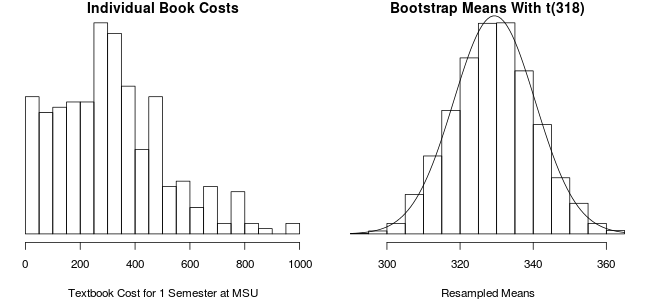
\includegraphics[width=\linewidth]{../plots/bookCostDistns.png}
The second plot is overlaid with a $t_{318}$ density curve.  Note how
it gives a very similar distribution to the bootstrap resampled means,
even though the original data is not symmetric.

We needed many bootstrap samples to get  the
``standard deviation'' of the resampling distribution.  Now we will use a
formula for the standard error (SE) of the sample mean, $\xb$ based on
sample size and the standard deviation of the raw data.  
$$SE(\xb) = \frac{s}{\sqrt{n}}$$
In the left-hand plot above, the spread of the individual points is $s
= 202.93$. The resampled means have spread of 11.20 which is quite
close to $SE(\xb) = 202.93/\sqrt{319} = 11.36$.  
\begin{itemize}
\item {\bf Standard Deviation} has several meanings:
  \begin{itemize}
    \item the spread of some  distribution, especially: the spread of
      individual  measurements.
    \item Population standard deviation with  Greek letter: $\sigma$,
    \item Sample standard deviation, $s$ from the formula: $s =
      \sqrt{\frac{1}{n-1}\sum(x_i - \xb)^2}$
    \item  Standard deviation of a statistic, for instance  $SD(\xb)
      =\sigma/\sqrt{n}$, is the true spread of the statistic.
  \end{itemize}

\item {\bf Standard error} is the estimated standard deviation of a
  statistic. Below is a table of the  standard deviations and standard
  errors we  are using.  Note how the SE just plugs an estimated value
  in to the SD formula.\\
  \begin{center}
  \begin{tabular}{|c|c|c|c|}\hline
    Statistic: & Standard Deviation & Test Std Error& CI Std Error\\ \hline
    $\phat$ & $\sqrt{\frac{p(1-p)}{n}}$ & $\sqrt{\frac{\phat(1-\phat)}{n}}$& $\sqrt{\frac{\phat(1-\phat)}{n}}$\\
    \hline
    $\phat_1 - \phat_2$&  $\sqrt{\frac{p_1(1-p_1)}{n_1}
      +\frac{p_2(1-p_2)}{n_2} }$ &
       $\sqrt{\frac{\phat_T(1-\phat_T)}(\frac{1}{n_1} + \frac{1}{n_2} )}$
       & $\sqrt{\frac{\phat_1(1-\phat_1)}{n_1}
          +\frac{\phat_2(1-\phat_2)}{n_2} }$ \\ \hline
     $\xb$ & $\frac{\sigma}{\sqrt{n}}$ & $\frac{s}{\sqrt{n}}$& $\frac{s}{\sqrt{n}}$ \\\hline
     $\xb_1 - \xb_2$ & $\sqrt{\frac{\sigma_1^2}{n_1} +\frac{\sigma_2^2}{n_2}} $
      & $\sqrt{\frac{s_1^2}{n_1} +\frac{s_2^2}{n_2}} $  
      & $\sqrt{\frac{s_1^2}{n_1} +\frac{s_2^2}{n_2}} $  \\ \hline
  \end{tabular}\vspace{.1in}    
  \end{center}
\end{itemize}

  Each of these $SD$'s and $SE$'s has sample size (square
  rooted) in the denominator.  As sample size gets big, $SD$ and $SE$ get
  smaller. More information leads to less variation.

  Add to this the fact that sample mean is an {\bf unbiased} estimator
  of the true population mean, and sample proportion is an {\bf
  unbiased} estimator of the true population proportion, and we see
  the power of using statistics to estimate parameters: larger sample
  sizes provide more information, less variation, and we can close in
  on the true parameter values. Here are two big ideas in statistics:

\subsection{  Law of Large Numbers}

\begin{center}
 \begin{fmpage}{.9\linewidth}
  In the long run, the sample mean $\xb$ will get closer and closer to the
   population mean, $\mu$, and the sample proportion $\phat$ will get
   closer and closer to the true proportion of successes, $p$.  You can define
   ``close'' as you wish -- the more precision needed, the greater the
   sample size.
 \end{fmpage}
\end{center}

  The {\bf LLN} addresses the width, or spread of the sampling
  distribution. The second important idea addresses the {\bf shape} of
  the sampling distribution, and was more of a surprise when it was
  discovered about 200 years ago (and proven, in general only 100
  years ago).


\subsection{  Central Limit Theorem} 

\begin{center}
\begin{fmpage}{.9\linewidth}
  As the sample size gets big, the shape
  of the sampling distribution of sample mean, $\xb$ gets closer and
  closer to a normal distribution.
\end{fmpage}
  \end{center}

The {\bf CLT} explains why the normal distribution is so useful.  Even if we
start with skewed data, like in the case of book costs, when we
average together 100 or more random values, the distribution of the
sample mean, $\xb$,  will approach a normal distribution.  It also
applies to proportions because if we record success as 1 and failure as
0, then $\phat$ is just the sample mean of the zeroes and ones.


%% Galton's Board here?


\subsection{ Assumptions for t-Procedures}


  Just as with proportions, all means methods require 
  \begin{itemize}
%%     \item The size of each sample must be less than a tenth the size
%%       of its population.
     \item Each sample must be representative of its population. 
     \item Independent samples and independent subjects within each
       sample.
  \end{itemize}
   In addition, we do need to examine the sample size {\bf and} shape
   of the sample data to determine if we can use $t$ procedures.
   \begin{itemize}
   \item For small sample sizes, we need distributions to be close to
     normally distributed: symmetric with no outliers.
   \item If sample size is 30 or more, we can use $t$ procedures
     unless the data are heavily skewed.
   \item If sample size is over 100, the Central Limit Theorem lets us
     use $t$ distributions even for heavily skewed data.
   \end{itemize}

   \begin{center}
     {\large\bf True or False:}
   \end{center}
   \begin{enumerate}
   \item \underline{\hspace{.5in}} The Law of Large Numbers says that the
     distribution of $\xb$  gets close to normal as $n$ gets big. 
   \item \underline{\hspace{.5in}} As degrees of freedom get big,
     $t$-distributions get 
     closer and closer to the standard normal distribution.
   \item \underline{\hspace{.5in}} The Central Limit Theorem gives us the shape of
     the distribution of $\xb$ for large $n$.
   \item \underline{\hspace{.5in}}  With larger sample size, we have better
     information about population parameters.
   \item \underline{\hspace{.5in}} Statistics from larger samples are less biased
     than those from smaller samples.
   \end{enumerate}

\begin{center}
  {\large\bf Confidence Interval for $\mu$}
\end{center}

With text book costs, we had:
$$ n = 319, \mbox{\hspace{1in}} \xb = 329.44, \mbox{ and\hspace{1in}}  s = 202.93 $$

With one sample, we use $n-1$ as the ``degrees of freedom'' for the t
distribution.  
\begin{enumerate}
  \setcounter{enumi}{5}
\item In the web app
  \url{http://shiny.math.montana.edu/jimrc/IntroStatShinyApps} select
  \fbox{t distribution} under \fbox{One Quant}. Change the degrees of
  freedom to \fbox{318}, then enter the probabilities for the
  \fbox{center} to find the $t^*_{318}$ multipliers to use in the
  formula for confidence interval:
     $$  \mbox{estimate} \pm t^*_{df} SE(\mbox{estimate}) $$
\begin{students}
   \begin{tabular}{l|rrrrr}
    Confidence level: &  \hspace{1cm}80\% &  \hspace{1cm}90\% &  \hspace{1cm}95\% & \hspace{1cm} 98\% & \hspace{1cm} 99\% \\ \hline
    $t_{318}^*$ cutoff  &  &  & 1.967 &  & 
  \end{tabular}\vspace{.2cm}
\end{students}
\begin{key}
   \begin{tabular}{l|rrrrr}
    Confidence level: &  \hspace{1cm}80\% &  \hspace{1cm}90\% &  \hspace{1cm}95\% & \hspace{1cm} 98\% & \hspace{1cm} 99\% \\ \hline
    $t_{318}^*$ cutoff  &1.284  &1.65  & 1.967 &2.338& 2.591
  \end{tabular}\vspace{.2cm}
\end{key}

 \item 
   How different are these from the values you found for the z
   distribution last week?
\begin{students}
  \vspace{1cm}
\end{students}
\begin{key}
\\ {\it Just a touch wider}
\end{key}
\item Find the margin of error and build a 90\% confidence interval
  for the true book cost.   
\begin{students}
  \vspace{1cm}
\end{students}
\begin{key}
\\ ME = $ 1.65 \times 202.93\sqrt{319} =18.747$ the 90\% CI is $
329.44 \pm 18.747 = (310.69, 348.19)$
\end{key}
\item Interpret the interval. 
\begin{students}
  \vspace{1cm}
\end{students}
\begin{key}
\\ {\it We are 90\% confident that the true mean amount spent on
  textbooks by some group of students is between \$310.69 and \$348.19.}
\end{key}
\item To what group of students does this inference apply? 
\begin{students}
  \vspace{1cm}
\end{students}
\begin{key}
\\ {\it Trick question: This was not a random sample of MSU
  students. It really just applies to the students in the sample.}
\end{key}

\end{enumerate}


\begin{center}
  {\large\bf Hypothesis Test}
\end{center}
We do not have a hypothesized value to use for true mean textbook
cost, so let's look at a different situation to do a hypothesis test
on one mean.  An article in the {\it Journal of American Medical
  Association} in 1992 provided data to challenge the long held belief
that ``normal'' human body temperature is $98.6^o$F.\footnote{
Mackowiak, P. A., Wasserman, S. S., \& Levine, M. M. (1992). A
critical appraisal of 98.6 F, the upper limit of the normal body
temperature, and other legacies of Carl Reinhold August
Wunderlich. {\it JAMA}, 268(12), 1578-1580.}  Research before this study was
published led the researchers to believe that ``normal'' for most
people is lower than $98.6^o$.


\begin{enumerate}
\setcounter{enumi}{10}
\item  What are the null and alternative hypotheses?  
\begin{students}
\\$H_0$:  \vspace{1cm}\\
$H_a$:  \vspace{1cm}
\end{students}
\begin{key}
\\ $H_0:\ \ \mu = 98.6$\\
$H_a:\ \ \mu<98.6$
\end{key}

Check these with another group, because being off on
direction will mess us up later.

\item  
Go to the same web app we've been using and choose the pre-loaded
\fbox{bodytemp} data under \fbox{One Quant} which contains these values:
\begin{verbatim}
temp
97.3 97.3 97.7 97.8 98.4 99.8 96.7 98.1 98.7 97.5
97.9 98.1 97.8 98.5 98.8 98.7 99.4 97.8 98.6 98.7
\end{verbatim}
 Obtain the mean and standard deviation ($s$). Use 3 decimal
  place accuracy throughout.
\begin{students}
  \vspace{1cm}
\end{students}
\begin{key}
\\ $\xb = 98.18$,  $s = 0.747$
\end{key}

\item Compute $SE(\xb)$.
\begin{students}
  \vspace{1cm}
\end{students}
\begin{key}
\\ {\it $0.747/\sqrt{20} = 0.167$}
\end{key}

\item How many standard errors is $\xb$ from $\mu_0$?  Compute the
  test statistic. 
\begin{students}
  \vspace{1cm}
\end{students}
\begin{key}
\\ {\it $ \frac{98.180 - 98.6}{0.167} = -2.514$}
\end{key}


\item Which $t$ distribution should we use?
\begin{students}
  \vspace{1cm}
\end{students}
\begin{key}
\\ {\it $t$ with 19 df}
\end{key}



\item Pull up the t-distribution web app and put the t-statistic into
  the top box and set the degrees of freedom you found just
  above. Check the direction of your alternative hypothesis and give
  the p-value for the test.
\begin{students}
  \vspace{1cm}
\end{students}
\begin{key}
\\ {\it 0.011}
\end{key}
\item  How strong is the evidence against $H_0$?  State your
  conclusion at the $\alpha = 0.04$ significance level.
\begin{students}
  \vspace{1cm}
\end{students}
\begin{key}
\\ {\it Very strong. We reject $H_0$ and conclude that true mean
  ``normal'' body temperature is less than $98.6^o$ F}
\end{key}

\item Based on your p-value, will a 96\% confidence interval for true
  mean body temperature contain 98.6?
\begin{students}
  \vspace{1cm}
\end{students}
\begin{key}
\\ {\it No. It is not a plausible value based on this sample.}
\end{key}

\item Build the 96\% CI.  Be sure to show which $t^*$ you use.
\begin{students}
  \vspace{1cm}
\end{students}
\begin{key}
 {\it $t^*_{19} = 2.2047$, 96\% CI $= 98.18 \pm 2.2047 \times 0.167 =
   (97.81, 98.55)$} 
\end{key}

\item Write up a report on  your hypothesis test of ``Normal'' body
  temperature.  You 
  may assume that these temperatures are from a random sample of US
  men and women aged 20 to 40 years old. (With one only group we do not make
  comparisons in the report.)
\begin{students}
  \newpage
\end{students}
\end{enumerate}



\begin{center}
  {\large\bf Take Home Message}
\end{center}
 
\begin{itemize}
\item Larger sample sizes are generally better than smaller ones --
   as long as they are representative.  If we are using a biased
   sampling method, no amount of increasing sample size will fix the
   bias problem.
 \item As sample size, $n$ gets big:
   \begin{itemize}
   \item statistics get closer to their respective parameters.
   \item distributions of means get closer to normal in shape.
   \item t-distributions get closer to Z (N(0,1)) because degrees of
     freedom are related to sample size.
   \end{itemize}
 \item Generic confidence interval:
  $$ \mbox{estimate} \pm \mbox{multiplier} SE(\mbox{estimate})$$
    for a single mean:
  $$ \xb \pm t^*_{n-1} SE(\xb)$$
  \item Test statistic:
   $$ t = \frac{\xb - \mu_0}{SE(\xb)};\ \ SE(\xb) =
   \frac{s}{\sqrt{n}}$$
    Compare to a $t_{n-1}$ distribution to get p-values.

 \item What questions do you have?  Write them here.\vfill

\end{itemize}




%% 4 pages. Too short? Add Galton's bd? est assumptions.
\begin{center}
  {\large\bf Assignment}
\end{center}

\begin{itemize}
\item Fill in the bottom 3 boxes in column 2 of the Review Table. 
%\item D2Quiz 11 is due April 18.  Take it on D2L.
 %%  We strongly encourage you to get help in the Math Learning Center.
\item Watch videos assigned on D2L.
%\item Watch the videos 14 \& 15 under Unit 3 Examples.
\item Read the next four pages before your next class.
\end{itemize}
  %%  t-distn for 1 mean  pgs  203-210


 \newpage

\fancyhead[LE,RO]{
   {\it Notes }\\
   {\it Unit \unitNum\   \ Page \thepage }
}
%Intentionally left blank
\phantom{No text here}
\newpage

\fancyhead[LE,RO]{
   {\it \theTopic }\\
   {\it Unit \unitNum\   \ Page \thepage }
}
  \def\theTopic{Reading 21 }

\section{  Which tool to use?}


In Unit 3 so far we have used the following tools:
\begin{enumerate}
\item Normal-based tests on a single proportion.
\item Normal-based confidence interval estimates of a single proportion.
\item Normal-based tests for equivalence of two proportions.
\item Normal-based confidence intervals to estimate the difference
  between two proportions.
\item t-based tests on a single mean
\item t-based CI's to estimate a single mean
\item t-based tests for the equality of two means  (coming up next)
\item t-based CI's to estimate a difference in means (coming up next)
\end{enumerate}

Below are reports of three studies. You will be asked to find the
appropriate tool for each situation.

\begin{alist}
\item ``Effects of Insulin in Relatives of Patients with Type 1
  Diabetes Mellitus'' by the Diabetes Prevention Trial–Type 1 Diabetes
  Study Group published in {\it N Engl J Med} 2002; 346:1685-1691

  \begin{list}{}{}
  \item [\bf Background]
    It is unknown whether insulin therapy can delay or prevent
    diabetes in nondiabetic relatives of patients with diabetes. 
  \item [\bf Methods]
    In a randomized, controlled, nonblinded clinical trial, we
    screened 84,228 first-degree and second-degree relatives of
    patients with diabetes for islet-cell antibodies and identified
    339 who had a projected five-year risk of becoming diabetic of
    more than 50 percent; they were randomly assigned to undergo
    either close observation (n = 170) or an intervention (n = 169)
    that consisted of low-dose subcutaneous ultralente insulin,
    administered twice daily for a total dose of 0.25 unit per
    kilogram of body weight per day, plus annual four-day continuous
    intravenous infusions of insulin. Oral glucose-tolerance tests
    were performed every six months. Median follow-up was 3.7 years.
  \item [\bf Results]
    Diabetes was diagnosed in 69 subjects in the intervention group
    and 70 subjects in the observation group. 
  \end{list}
  \begin{enumerate}
   \item What is the researchers' question?\vspace{1cm}
   \item What two variables will be used in the analysis?\vspace{1cm}
   \item What is the parameter of interest?\vspace{1cm}
   \item Which two of the tools listed above are appropriate for these
     data? Explain why.\vspace{2cm}
   \item Just based on the reported results, do you expect a test to
     give a large or small p-value?  Why?\vspace{1cm}
   \item Again, without doing the analysis, we would expect a 90\%
     confidence interval for some parameter to contain zero.  What
     parameter? \vspace{1cm}
  \end{enumerate}
% \item [Debunking the Myths Commonly Believed to Affect Test Performance
%   among College Students]
\item ``The Effects of Text Messaging During Dual-Task Driving Simulation on Cardiovascular and Respiratory Responses and Reaction Time''
  by:  	Park, Andrew; Salsbury, Joshua; Corbett, Keira; Aiello,
  Jennifer. 
  from: {\it Ohio J Sci} 111 (2-5): 42-44 

  \begin{list}{}{}
  \item [\bf Abstract]
    Research over the past decade has shown the potentially harmful
    effects of distracted driving, particularly on reaction time of
    the driver to external stimuli. With the recent surge in frequency
    of the use of cell phones for text messaging in nearly all
    situations, including during driving, it is important to
    understand the impact of texting on driver reaction time and the
    body’s physiological response. This study attempts to replicate
    the effects of text messaging distractions on reaction times found
    in previous studies.
  \item [\bf Methods]
    The 40 subjects in this IRB approved study were students at Ohio
    Northern University between the ages of 18 and 22 who used their
    cell phones daily for texting purposes. All subjects refrained
    from caffeine and alcohol consumption for a minimum of 24 hours
    prior to testing.

    ST (single task): Each was seated with both hands next to but not
    touching the 
    computer mouse and forearms resting on the desk. The subject would
    click the mouse each time the stoplight changed from red to
    green. Subjects would then reposition their arms to the original
    position. The test allowed for five reaction time (RT) trials to be taken
    consecutively over the course of approximately one minute with
    random rest intervals as determined by the test.  The test then
    automatically calculated mean RT in seconds (s).

    DT (dual task): After a five-minute rest period, subjects repeated
    the RT test with dual-task conditions. Each participant was seated
    with forearms resting in the same manner, but with both hands
    holding their phone next to but not touching the mouse. A typed
    sheet of paper with questions asking for the participant’s full
    name, age, address, and contents of last meal was taped to the top
    of the computer screen, but not obstructing the participant’s view
    of the stoplight.  This position simulated the shift in visual
    attention a driver would experience while attempting to text and
    drive. Participants were not allowed to read the questions prior
    to testing. Once the test began, subjects were to read the
    questions and respond to as many as possible in a texted message
    while maintaining visual focus on his or her phone while
    texting. This was done while simultaneously completing the
    reaction test, requiring participants to remove one hand from the
    phone to click the mouse in response to stimuli. Again, five
    trials were taken and the mean recorded as his/her dual-task (DT)
    reaction time.  Means for all participants in ST and DT conditions
    were compared using an unpaired two-tailed test (N=40).
  \item [\bf  Results]\ \ \\
   ST mean = 0.51 sec, SD = 0.41 sec\\
   DT mean = 1.22 sec, SD = 0.36 sec
 \end{list}
   \begin{enumerate}
   \item What is the researchers' question?\vspace{1cm}
   \item What two variables will be used in the analysis?\vspace{1cm}
   \item What is the parameter of interest?\vspace{1cm}
   \item Which two of the tools listed above are appropriate for these
     data? Explain why.\vspace{2cm}
   \item Just based on the reported results, do you expect a test to
     give a large or small p-value?  Why?\vspace{1cm}
   \item Again, without doing the analysis, we would guess that a 90\%
     confidence interval for some parameter would not contain zero.  What
     parameter? \vspace{1cm}
  \end{enumerate}

\item ``Texting while driving using Google Glass$^{TM}$: Promising but not
  distraction-free.'' by: He, Jibo, et al. in: {\it Accident Analysis
    \& Prevention} {\bf 81} (2015): 218-229.\\
  \begin{list}{}{}
  \item [\bf Abstract] Texting while driving is risky but common. This
    study evaluated how texting using a Head-Mounted Display, Google
    Glass, impacts driving performance. Experienced drivers performed
    a classic car-following task while using three different
    interfaces to text: fully manual interaction with a head-down
    smartphone, vocal interaction with a smartphone, and vocal
    interaction with Google Glass. Fully manual interaction produced
    worse driving performance than either of the other interaction
    methods, leading to more lane excursions and variable vehicle
    control, and higher workload. Compared to texting vocally with a
    smartphone, texting using Google Glass produced fewer lane
    excursions, more braking responses, and lower workload. All forms
    of texting impaired driving performance compared to undistracted
    driving. These results imply that the use of Google Glass for
    texting impairs driving, but its Head-Mounted Display
    configuration and speech recognition technology may be safer than
    texting using a smartphone.
  \item [\bf Highlights]
    \begin{itemize}
    \item Texting using Head-Mounted and Head-Down Displays both
      impair driving performance.
    \item Texting vocally is less disruptive to driving than texting manually.
    \item Texting using Head-Mounted Display is less distracting than Head-Down Display.
    \item Speech recognition and Head-Mounted Display can potentially reduce distractions.
    \end{itemize}
  \item [\bf Methods] Twenty-five students (12 males and 13 females; M
    = 20.48 years, SD = 2.14 years, ages range from 18 to 25 years)
    from Wichita State University participated in the driving
    experiment for course credit.
  
    This study used a classic car following task on a driving
    simulator. One recorded response was how well the driver stayed in
    the lane as measured by the number of incursions into another lane.
  \end{list}
  Suppose that you are a researcher in driving safety and already have
  lots of data about how well people perform this task when not
  texting. In fact, we will assume the mean for the non-texting
  population is 3.1.  You want to know if this mean also holds for
  people who are texting through Google Glass.
   \begin{enumerate}
   \item What one variable will be used in the analysis?\vspace{1cm}
   \item What is the unknown parameter of interest?\vspace{1cm}
   \item Which two of the tools listed above are appropriate for these
     data? Explain why.\vspace{2cm}
   \item Of the two possible tools, Which will more directly answer
     the research question? Why? \vspace{1cm}
  \end{enumerate}

\end{alist}






   %%   t-distn examples & practice 
                                %%   p 211-214 buff  
\newpage


\fancyhead[LE,RO]{
   {\it Notes }\\
   {\it Unit \unitNum\   \ Page \thepage }
}
%Intentionally left blank
\phantom{No text here}
\newpage

\fancyhead[LE,RO]{
   {\it \theTopic }\\
   {\it Unit \unitNum\  Activity \dayNum \ Page \thepage }
}
 \def\theTopic{Energy Drinks II}
\def\dayNum{25 }


\section{More Energy Drinks with t-tests}


Back on Activity 14 we compared an energy drink with
alcohol, REDA, to a control.  Our conclusion that ``change in RBANS''
was lower in the REDA group did not allow us to say whether that was
due to the alcohol 
or the stimulant in REDA.  The two  explanatory variables were
``confounded'' meaning that we can't separate the effects.  The
researchers knew this would be a problem, so they included a third
group in the study: 9 randomly assigned women got RED, an energy drink
with no alcohol.  Today we'll compare RED and control means using
confidence intervals and hypothesis tests based on a $t$
distribution. 

  The research question is: 

  {\sf
    Does neuropsychological performance (as measured on the RBANS
    test) change after drinking an energy drink? }

   Higher RBANs scores indicate better memory skills.

 Go to the usual website and use the pre-loaded {\tt REDvsControl}
 data set under \fbox{One of Each}.

  \begin{enumerate}
  \item  Obtain ``Actual'' Mean and Std dev for each group. 
\begin{students}
    \vspace{4cm}    
\end{students}

\begin{key}
  {\it Means:  control: 1.219, RED: -2.44 \\%, REDA:  -8.39\\
       Std.dev.: control: 3.919, RED: 6.425}%, REDA, 10.02} 
\end{key}

\item Using t-based methods requires that we either have ``near
  normal'' data or  large sample sizes.  Do you see extreme outliers
  in the plots?  Are the data skewed?

\begin{students}
    \vspace{2cm}    
\end{students}

\begin{key}
  {\it  These look OK to me, though the spreads do not look equal.}
\end{key}

\end{enumerate}


There are no really obvious problems with the assumptions, so we will
proceed to compare RED to Control  using a hypothesis test.

%\newpage
\begin{enumerate}
\setcounter{enumi}{2}

\item  What are the null and alternative hypotheses when comparing RED
  to Control? Use notation, and write them out with words.
  Do not assume they knew ahead of time which  mean would be
  larger. \\
\begin{students}
 $H_0:$    \vspace{1cm}    \\ $H_a:$    \vspace{1cm}
\end{students}
\begin{key}
  {\it   $H_0:\ \mu_1 = \mu_2$ The mean change in RBANS is the same
    for treatment (RED) and Control.    \\ $H_a: \mu_1 \neq \mu_2$ The
    mean change in RBANS is not the same for treatment (RED) and control.  }
\end{key}

   Check with another group to be sure we have the correct
   direction for $H_a$.

\item  Let group 1 be Control and group 2 be RED. Compute $SE(\xb_1 -
  \xb_2) = \sqrt{\frac{s_1^2}{n_1} +     \frac{s_2^2}{n_2}}$. 
\begin{students}
    \vspace{2cm}    
\end{students}

\begin{key}
  {\it  $ \sqrt{\frac{3.92^2}{9} +    \frac{6.43^2}{9}} = \sqrt{1.707
    +4.594} = 2.5102$.} 
\end{key}
\item As with a single mean, our test statistic is called $t$ and is
  found by dividing  the difference between sample statistic and its
  value under $H_0$ by its $SE.$  Find t. \\
\begin{students}
  $ t = \frac{\xb_1 - \xb_2 - (\mu_1 - \mu_2)}{SE(\xb_1-\xb_2)} = $
    \vspace{2cm}    
\end{students}

\begin{key}
   $ t = \frac{\xb_1 - \xb_2 - \mu_1 - \mu_2}{SE(\xb_1-\xb_2)} = 
          \frac{ 1.219-( -2.44)}{2.5102} = 1.458 $
\end{key}

\item We need to figure out which degrees of freedom for our t
  test. When working with two means, we take the smaller sample size
  and subtract one from it. What is that for the Energy Drinks study?
  ({\small This is a conservative approach. Other books or software
    programs might use a different number.})
\begin{students}
    \vspace{2.6cm}    
\end{students}

\begin{key}
  {\it  8}
\end{key}

 \item  Go to the t distribution part of the applet and put your t
   test statistic in the top box, 
   set its degrees of freedom, and select the correct direction for the
   alternative.  What is our p-value?  State your decision and 
   conclusion about these two drinks. 
\begin{students}
    \vspace{5cm}    
\end{students}

\begin{key}
  {\it 0.182. At any of the commonly used $\alpha$ levels, we fail to
    reject the null hypothesis that mean change in RBANS score is the
    same for control and RED groups.  There is not sufficient evidence
    to say that they differ.}
\end{key}


 \item  Next we want to compare RED drinkers to REDA drinkers (group 2
   to group 3). 

   \begin{enumerate}
     \item Your null and alternative hypotheses are the same, but we
       need to use subscripts 2 and 3 instead of 1 and 2.  Copy them
       here. 
\begin{students}
    \vspace{2cm}    
\end{students}

\begin{key}
  {\it   $H_0:\ \mu_2 = \mu_3$ The mean change in RBANS is the same
    for RED and REDA.    \\ $H_a: \mu_2 \neq \mu_3$ The
    mean change in RBANS is not the same for RED and REDA.  }
\end{key}
 

      \item Compute the difference in means.
\begin{students}
    \vspace{1cm}    
\end{students}

\begin{key}
  {\it  $ -2.44 -( -8.329) = 5.889$}
\end{key}

      \item Compute the $SE$ of the estimator.
\begin{students}
    \vspace{1cm}    
\end{students}

\begin{key}
  {\it  $ \sqrt{ \frac{6.43^2}{9} + \frac{10.02^2}{9}} = \sqrt{
    4.594 + 11.1566 } = 3.969$ }
\end{key}

      \item Compute the $t$ test statistic.
\begin{students}
    \vspace{1cm}    
\end{students}

\begin{key}
  {\it   $ 5.889 / 3.969 = 1.484$}
\end{key}

      \item What degrees of freedom will you use?  Find the p-value.
\begin{students}
    \vspace{1cm}    
\end{students}

\begin{key}
  {\it  8 df.  The p-value is $2 \times 0.088 = 0.172 $}
\end{key}

      \item What is your decision? your conclusion? 
\begin{students}
    \vspace{2cm}    
\end{students}

\begin{key}
  {\it  Again, we do not have much evidence against the null
    hypothesis that the two groups have the same mean. We fail to
    reject $H_0$ at all commonly used $\alpha$ levels. }
\end{key}

     \end{enumerate}

     \begin{center}
       {\large\bf Confidence Interval}

 Reminder. The general form of a t-based CI is:
     \end{center}
  $$ \mbox{estimate} \pm t^*_{df} \times SE(\mbox{estimate}) $$ 

 \item Finally, we'll go back to the original comparison between REDA
   and Control means. However, we'll set this one up as a confidence
   interval instead of a t-test. 
   \begin{enumerate}
   \item Compute the difference in means between REDA and control.
\begin{students}
    \vspace{.5cm}    
\end{students}

\begin{key}
  {\it  $1.219-( -8.329) = 9.548 $}
\end{key}

   \item Compute  $SE(\xb_1-\xb_3)$
\begin{students}
    \vspace{.5cm}    
\end{students}

\begin{key}
  {\it $\sqrt{ \frac{3.919^2}{9} + \frac{10.02^2}{9}}= 3.587$}
\end{key}

   \item What degrees of freedom do we need?\\ 
\begin{students}
    \vspace{.5cm}    
\end{students}

\begin{key}
  {\it  8 df.   $t^* = 2.306 $}
\end{key}
     Use the web app to find the $t^*$ multiplier for a 95\% 
     confidence interval.
\begin{students}
    \vspace{.5cm}    
\end{students}

\begin{key}
  {\it  8 df.   $t^* = 2.306 $}
\end{key}

   \item Find the margin of error and construct the 95\% CI.  Does it
     contain zero?  If testing 
     $H_0: \mu_1 = \mu_3$ versus a two-sided alternative at the
     $\alpha = 0.05$ level, would you reject $H_0$?  Explain.
\begin{students}
    \vspace{3cm}    
\end{students}

\begin{key}
  {\it  ME $=2.306 \times 3.587 =8.272 $, 95\% CI:   $9.548 \pm  
    8.272 = ( 1.28, 17.82)$ Zero is not in the interval, so it is not
    a ``plausible value'' for the difference in means.  We would
    reject the null in favor of the alternative at $\alpha = 0.05$.  }
\end{key}

   \end{enumerate}

 \item   How do you explain the fact that two of the three
   t-tests we've done gave large p-values and another gave a small p-value? Is
   that inconsistent? 
\begin{students}
    \vspace{3cm}    
\end{students}

\begin{key}
  {\it  The confidence interval shows that we have
    fairly strong evidence that the mean for control change in RBANs is
    larger than the mean for REDA change in RBANS. We do not have very
    large sample sizes in this study, so it is not surprising that two
    comparisons found that the middle mean (RED) was not very
    different from either extreme (Control or REDA), yet the two
    extreme values were far enough apart to detect a fairly strong
    difference. }
\end{key}

\item Could the difference in REDA and Control means be just due to
  random chance?  Explain.
\begin{students}
    \vspace{2cm}    
\end{students}

\begin{key}
  {\it Yes.  Our conclusions do not change just because we've used a
    different method to compute the p-value.  It's still possible that
  one group was higher just due to random assignment of treatment.}
\end{key}
\begin{students}
    \vspace{2cm}    
\end{students}

\begin{key}
  {\it Yes.  Our conclusions do not change just because we've used a
    different method to compute the p-value.  It's still possible that
  one group was higher just due to random assignment of treatment.}
\end{key}
\item Can we make causal inference about the effects of energy drinks
  and alcohol?
\begin{students}
    \vspace{2cm}    
\end{students}

\begin{key}
  {\it  Yes.  Because treatments were randomly assigned, it is very
    unlikely that we would see such large differences just by chance,
    so the observed differences (or lack thereof) are attributable to
    the treatments.  }
\end{key}


\item Write up the hypothesis test results as a report.  Include all
  three comparisons we've made. \vfill
   
 \end{enumerate}
 \newpage

\begin{center}
  {\large\bf Take Home Message}
\end{center}

\begin{itemize}
  \item Interpretation of results does not change just because we
    switched from permutation testing to t-tests.  We still ask ``Was
    this a random sample of subjects?'' to obtain inference back to a
    population, and we still ask ``Were treatments assigned at
    random?'' to conclude that change in one variable caused changes
    in the other. 
  \item The t-test approach uses formulas for standard errors, while
    the permutation test relies on repeated permutations or resampling
    to get the same information about the spread of the sampling
    distribution under $H_0$.  Both work!
  \item We can use t-tests to compare two means, but do have to be
    careful with small sample sizes.  We should not use t-tests with
    sample sizes less than 15 unless the data look symmetric with no
    outliers.
  \item With large sample sizes, t methods are robust to outliers and
    skewness.
  \item When sample sizes are small, only {\em large} differences will
    be flagged as having ``strong evidence''.  We'll look at this
    later in more detail.
  \item What questions do you have?  Write them here.  \vfill
\end{itemize}



\begin{center}
  {\large\bf Assignment}
\end{center}

\begin{itemize}
\item Fill in the bottom 3 boxes in column 4 of the Review Table. 
% \item D2Box 11 is due April 21. (The last D2Box assignment.)  Turn in
%   a pdf file to the DropBox on D2L.
 %%  We strongly encourage you to get help in the Math Learning Center.
\item Watch   videos 16 and 17 under Unit 3 Examples.
\item Read the next two pages before your next class.
\end{itemize}
   %% more REDs  pg  215 - 220
  \newpage


\fancyhead[LE,RO]{
   {\it \theTopic }\\
   {\it Unit \unitNum\   \ Page \thepage }
}
  \def\theTopic{Reading 22 }

\section{ Seeing Double}


One of the assumptions for doing any statistical inference in this
course is that we have independent observations.  
We have also seen situations in which researchers obtained two
measurements on one unit:
\begin{enumerate}
  \item  When assessing the effect of energy drinks and alcohol on
    people, researchers measured each subject before and after they
    drank the beverage.  The two measurements on the same person are
    not independent because some people will tend to score high each
    time and others will tend to score low.
  \item Texting study ``B'' on page 191 of the last reading used each
    subject for the ST  condition and for DT condition.  
    \begin{enumerate}
    \item Are the two  observations independent?\vspace{1cm}
    \item If not, what characteristics of the person would affect both
      observations? \vspace{1cm}
    \end{enumerate}
  \item Similarly, study ``C'' on page 192-193 observed drivers on a
    driving simulator under several conditions (no texting, texting
    manually, texting with Google Glass).  The same issues with
    independence occur for this study as well.
  \end{enumerate}

It might sound like we don't recommend measuring people multiple
times, but actually, \vspace{.4cm}

{\bf it's a good idea to take multiple measurements on people.}\vspace{.4cm}
  

If you read the ``Energy Drinks'' study carefully, you'll see that we
did not analyze the RBANS scores individually, but subtracted post
score minus pre-score and analyzed ``Change in RBANS''.
\begin{itemize}
\item How many ``change in RBANS'' scores did we have for each
  person?\vspace{.5cm}
\item Are the ``change in RBANS'' measurements independent?\vspace{.5cm}
\end{itemize}

{\bf Take differences to get a single difference or change for each
  subject.} Then we have just one ``change'' per subject, and, as long
as one subject doesn't influence another, we can assume observations
are independent.  


Simple example:\\
  In the texting study ``B'' on page 191, each subject was tested
  under both DT (while texting) and ST (no texting) conditions.  We
  don't know why the authors specifically stated that they used an
  ``unpaired'' t-test, because this seems to be a situation where
  pairing should be used.  

  One should subtract one average reaction time from the other and
  analyze the differences as a one-sample t-test (or compute a
  one-sample t-based confidence interval) to make a statement about
  the mean difference, which can extend our inference to answer
  questions about the impact of texting while doing another task in a
  whole population of students.\vspace{.4cm}

The {\bf Paired T test} is really nothing new. 
\begin{itemize}
\item Take differences for each subject or unit.
\item Analyze the differences using one-sample t procedures. Degrees
  of freedom will be $n-1$, sample size minus one.
\end{itemize}
One caution: do be careful in stating results. 
Talk about the mean change or the mean difference, not the difference
in means (because we are using one sample methods, there is only one
mean, but it's the mean of the change in scores or the mean of the differences.)


{\bf Blocking}\\
  One of the principles of experimental design from page 73 is
  ``blocking'' which means that we like to compare treatments on units
  which are as alike as possible.  The paired t-test uses each subject
  as one block, then condenses two observations per person down to a
  single difference.
 
{\bf Randomization}, another principle of experimental design, is
still important.  We wish that the texting study ``B'' had randomly
assigned  subjects to either ST or DT for their first experience
 instead of giving them all in the same order.  What lurking
variable  might change reaction times under the two conditions, but
could be ``evened out'' by randomly changing the order?\vspace{1cm}

A local company selling diet aides likes to advertise in the newspaper
showing pictures of someone who lost 75 pounds while using their
products.  
\begin{itemize}
 \item Should a person who would like to lose weight be heavily
   influenced by stories of one person's weight loss?\vspace{1cm}
 \item What evidence would be more impressive?\vspace{1cm}
 \item How would the ideas above be used to demonstrate the
   effectiveness of a dieting product?\vspace{.2cm}
\end{itemize}



\begin{center}
  {\large\bf Important Points}\vspace{-.5cm}
\end{center}
   
\begin{itemize}
  \item Know the assumptions for using $z$ and $t$ methods. \vfill
  \item It is a good idea to collect multiple observations on
    individuals under different treatment conditions, but before
    analyzing them, we should reduce them down to a single number per
    subject.\vfill
  \item We use one-sample t procedures to analyze differences. DF =
    $n-1$. \vspace*{1cm}
\end{itemize}

   %%  Intro 2 pairs?  p 221 -222 buff  


\fancyhead[LE,RO]{
   {\it Notes }\\
   {\it Unit \unitNum\   \ Page \thepage }
}
%Intentionally left blank
\phantom{No text here}
\newpage


\fancyhead[LE,RO]{
   {\it \theTopic }\\
   {\it Unit \unitNum\  Activity \dayNum \ Page \thepage }
}
 \newpage
 \def\theTopic{Pairing }
\def\dayNum{26 }


\section{ Are You Two Together?  -- Pairing}


  % When we want to make comparisons, and the data include lots of
  % excess noise, {\bf pairing} is a way to get ``cleaner'' or more
  % precise comparisons.

   In the ``Energy Drinks'' study we've looked at
  several times, each participant took a test  before the
  experiment really began. She  returned about 10 days later, and was
  randomly assigned a treatment (RED, REDA or Control) and was again
  given a very similar test.  The response variable we looked at
  was her ``change in RBANS'', meaning we subtracted the first test
  score from the second.   
  \begin{enumerate}
  \item The ``Repeatable Battery for the Assessment of
    Neuropsychological Status'' outputs scores for immediate memory,
    visuospatial/construction, language, attention, and delayed
    memory.  Discuss: What attributes of a person would make her score
    higher or lower?  Write down two or three of your best guesses.
\begin{students}
    \vspace{2cm}    
\end{students}

\begin{key}
  {\it Intellect, sleepiness, memory, motivation.}
\end{key}


%   \item Write down an estimate of how much a person's attribute will
%     change in 10 days for each of the attributes above.  Think of how
%     much one person changes relative to differences between different
%     people (take $\sigma = 4$ to be the spread from person to person). \begin{students}
%     \vspace{2cm}    
% \end{students}

% \begin{key}
%   {\it Intellect and memory do not change much from day to day
%     motivation could change a fair amount, and  sleepiness could
%     change a lot.}
% \end{key}


The ``Repeatable'' part of RBANS means that it comes in several
different versions which are all supposed to give the same scores to
the same people.  If the researchers had used exactly the same
questions, subjects might have learned from the first attempt and done
better the second time.


  \item  For each of the following situations, write ``paired'' if
    there is one sample measured twice or ``two samples'' otherwise.
    Ask your self: ``Does it make sense to take differences and
    analyze those? (paired) Or do we compute means from each of two groups?''
     Another clue: If sample sizes might be different, it's not
     paired. 
 
    \begin{enumerate}
    \item To study the effect of exercise on brain activity
      researchers recruited sets of identical twins in middle age.
      One twin was randomly assigned to engage in regular
      exercise and the other didn't exercise. 
\begin{students}
 \vspace{1cm}
\end{students}

\begin{key} Paired -- a pair of twins is the ``unit''
\end{key}


    \item To see if curriculum changes are effective, researchers took
      a sample of 100 eighth graders' standardized test scores from
      this year and compared them to a sample of 100 scores of last
      year's eighth graders (on the same exam).
\begin{students}
 \vspace{1cm}
\end{students}

\begin{key} Not paired -- 2 samples.
\end{key}


    \item In a study to determine whether the color red increases how
      attractive men find women, one group of men rated the
      attractiveness of a woman after seeing her picture on a red
      background and another group of men rated the same woman after
      seeing her picture on a white background.  
\begin{students}
 \vspace{1cm}
\end{students}

\begin{key} Not paired. The men form two samples - or treatment groups.
\end{key}


    \item To measure the effectiveness of a new teaching method for
      math in elementary school, each student in a class getting the
      new instructional method is matched with a student in a separate
      class on IQ, family income, math ability level the previous
      year, reading level, and all demographic characteristics.  At
      the end of the year, math ability levels are measured.
\begin{students}
 \vspace{1cm}
\end{students}

\begin{key} Paired -- artificially by matching case to control.
\end{key}
  

\item Each student in an intro stat class walked 100 yards twice. Once
  with arms down at his/her sides, another time while ``pumping'' arms
  up and down with each stride. The order of ``pumping'' or ``not''
  was randomized for each student.  Pulse (beats per second) was
  measured after each walk.
\begin{students}
 \vspace{1cm}
\end{students}

\begin{key} Paired. Two measurements on each student.
\end{key}


    \end{enumerate}
  \end{enumerate}
  {\bf Being Careful With Wording}:\\
  With paired data, we are making inference about the ``true mean of
  the differences.''  This is different from the wording we used with
  two independent samples. There we looked at the ``difference in true
  means'' -- which makes sense because we had two populations to
  compare. With paired data, we have a single sample of
  differences. The observations subtracted to get the differences were
  not independent because they came from the same subject, but the
  sample of all differences can be independent as long as one subject
  (or unit) did not influence another. 



   Now we'll analyze some paired data.

   \begin{center}
     {\large\bf Tears and Testosterone}
   \end{center}
    Do pheromones (subconscious chemical signals) in female
      tears {\bf change}  testosterone levels in men?\\
    Cotton pads had either real female tears or a salt solution
      that had been dripped down the same woman's face.
    Fifty men (a convenience sample) had a pad attached to their upper
    lip twice, once 
      with tears and once without, in random order.
    Response variable: testosterone level measured in
      picograms/milliliter, pg/ml.

    Take differences: Saline T--level minus Tears T--level.\\
    The mean of the differences is  $\overline{x}_D = -21.7$, and
    the spread of the differences is  $s_D = 46.5$ pg/ml.
    \begin{enumerate}
  \setcounter{enumi}{3}
        \item Test: ``Is the mean difference 0?''
          \begin{enumerate}
            \item Check the assumptions. If the differences are
              fairly symmetrically distributed, can we use t-procedures?
              Explain. 
\begin{students}
    \vspace{2.8cm}    
\end{students}

\begin{key}
  {\it  Yes. $n=50 > 30$ so we're OK. We have random ordering, and 
     subjects' responses should be independent.} 
\end{key}

        \item State hypotheses in terms of parameter $\mu_D$, the
              true mean of differences.
\begin{students}
    \vspace{2cm}    
\end{students}

\begin{key}
  {\it  $H_0: \mu_D = 0$ versus $H_a: \mu_D \neq 0$}
\end{key}

    {\bf STOP.  Check} the direction of the alternative with another group.
    \item Compute t statistic as for  testing $H_0:\ \mu_D=0$.
\begin{students}
    \vspace{1.5cm}    
\end{students}

\begin{key}
  {\it  $t^* = \frac{ -21.7}{46.5/\sqrt{50}} = -3.30 $}
\end{key}

            \item Do we use Normal  or t distribution? 
              If t how many df?
\begin{students}
    \vspace{1cm}    
\end{students}

\begin{key}
  {\it     $t$ with 49 df}
\end{key}

            \item Look up the p-value in a web app and give the
              strength of evidence.
\begin{students}
    \vspace{1.7cm}    
\end{students}

\begin{key}
  {\it  $2 \times .0009 = 0.0018$ This is very strong evidence against
  the null hypothesis.}
\end{key}

   \item At the $\alpha = .02$ level, what is your decision?
\begin{students}
    \vspace{1cm}    
\end{students}

\begin{key}
  {\it  Reject $H_0$.}
\end{key}


            \item Explain what we've learned in context. (Give scope
              of inference.  If outside observers would say the men
              studied were representative of all US men, how could the
              scope be extended?)
\begin{students}
    \vspace{1cm}    
\end{students}

\begin{key}
  {\it  We've found causal evidence that exposure to womens' tears
    does reduce testosterone levels in men. (p-value = 0.002). If this
  is a representative sample, then we can extend the inference back to
the population of US adult males.}
\end{key}

          \end{enumerate}
        \item Build a 90\% CI for the true mean difference, $\mu_D$.
          \begin{enumerate}
          \item Find the correct multiplier.
\begin{students}
    \vspace{1cm}    
\end{students}

\begin{key}
  {\it     $t^*_{49}  = 1.677 $ }
\end{key}
   \item  Compute the margin of error and build the interval.
\begin{students}
    \vspace{2cm}    
\end{students}

\begin{key}
$$ME = 1.677\times 46.5/\sqrt{50} = 1.677\times 6.58 = 11.03;
    \mbox{\hspace{.4in} CI: } -21.7 \pm 11.03 = (-32.7, -10.7) pg/ml$$
\end{key}

 \item Interpret the interval in context. What do you mean by ``confidence''?
\begin{students}
    \vspace{5cm}    
\end{students}

\begin{key}
  {\it  We are 90\% confident that the true mean difference in
    testosterone levels for men without and with exposure to womens'
    tears is in the interval (-32.7, -10.7) pg/ml. This says that the
    tears really did cause a decrease in T--levels in this group of
    men. Our confidence is in the process by which we built the
    interval.  When the procedure is used over and over, 90\% of
    intervals built this way (in the long run) will include their true
    mean.  }
\end{key}
          \end{enumerate}

   \item Designing a study: Researchers at the Western Transportation
     Institute (just south of the football stadium) use a driving
     simulator to test driver distractions (among other things). It is
     the front end of a car with large projection screens.  Suppose 
     they want to assess how distracting it is to read text messages
     on a phone while driving. The response they measure will be
     response time when a child suddenly runs out onto the road in
     front of the car.
     \begin{enumerate}
      \item How would they set this up to use  paired measurements?
\begin{students}
    \vspace{1cm}    
\end{students}

\begin{key}
  {\it Each driver does the same course twice -- once while reading a
    text and again without the phone.}
\end{key}
\item How could randomization be used?
\begin{students}
    \vspace{1cm}    
\end{students}

\begin{key}
  {\it Randomly (flip a coin?) select whether each driver gets the
    text reading first or second.}
\end{key}
\item Alternately, they could just test half their subjects
        while reading a text and half without the texting.  Which
        study design do you recommend?  Explain why.
\begin{students}
\vspace{4cm}
\end{students}

\begin{key}
  {\it Pairing seems like a good idea because some people have faster
    reaction times than others. By subtracting two reaction times you
    get rid of other effects such as age or sleepiness. }
\end{key}
\end{enumerate}

\item A study of the effects of drinking diet soda versus
  sugar--sweetened soda on weights of 32 adults used a ``cross--over''
  design in which each adult was given diet soda to drink for one six
  week period, and given sugar--sweetened soda to drink in another six
  week period.  The order of assignment was randomized for each
  participant.  The response measurement was ``weight gain'' over the
  six weeks.
  \begin{enumerate}
  \item It the parameter of interest the difference in true means or
    the true mean difference?  Explain.
\begin{students}
\vspace{3cm}
\end{students}

\begin{key}
  {\it True mean difference. This is a case of one sample measured
    twice.  We subtract weight gains (say sugar minus diet) so that
    our observations are independent of each other.}
\end{key}
\item How would you process the data in order to analyze it? 
\begin{students}
\vspace{2cm}
\end{students}

\begin{key}
  {\it Take difference in weight gain (diet minus sugar) for each person.}
\end{key}
\item What distribution would you use to find p-values or
    a confidence interval multiplier?
\begin{students}
\vspace{2cm}\newpage
\end{students}

\begin{key}
  {\it $t_{31}$}
\end{key}
\end{enumerate}

\end{enumerate}


\begin{center}
  {\large\bf Take Home Message}
\end{center}
\begin{itemize}
\item Taking two measurements on the same subjects is quite different
  from taking two samples or assigning two treatments. You need to
  read carefully to see how data were collected.  We do not have
  independent measures if they are on the same units.

  \item With two independent samples the parameter of interest was
    ``difference in true means.''  With a single sample measured
    twice, the parameter is ``true mean difference''.

  \item To analyze paired measures, take differences first (before
    averaging) and use the one-sample t procedures.

  \item Pairing is a good strategy for reducing variability.

  \item The Energy Drinks study has a lot going on.  They took
    differences first, to get ``change in RBANS'', but they also had
    three independent groups to compare: Control, RED, and REDA.

  \item What  questions do you have?  Write them here.\vfill
\end{itemize}


%% need more -- only 2 pages.

\begin{center}
  {\large\bf Assignment}
\end{center}

\begin{itemize}
\item Review for the final exam.
%\item D2Box 11 (last one) is due April 21st Turn in a pdf on D2L.
%\item D2Quiz 12 (last one) is due April 25.  Fill in your answers on D2L.
 %%  We strongly encourage you to get help in the Math Learning Center.
\item Read the next three pages before your next class.
\item Check D2L for videos and other assignemnts.
\end{itemize}
 %% Paired  %%   pgs 223 - 228
 \newpage


\fancyhead[LE,RO]{
   {\it \theTopic }\\
   {\it Unit \unitNum\   \ Page \thepage }
}
  \def\theTopic{Reading 23 }

\section{ Concussions in the News}



\begin{enumerate}
\item   Read the abstract from this  article.

Petraglia AL, Plog BA, Dayawansa S, Chen M, Dashnaw ML, Czerniecka K,
Walker CT, Viterise T, Hyrien O, Iliff JJ, Deane R, Nedergaard M,
Huang JH. (2014). ``The spectrum of neurobehavioral consequences after repetitive mild traumatic brain injury: a novel mouse model of chronic traumatic encephalopathy.''
{\bf J Neurotrauma} Jul 1; {\bf 31}(13):1211-24. 
\url{http://www.ncbi.nlm.nih.gov/pubmed/24766454}
{\footnotesize
\begin{quotation}
Abstract\\
There has been an increased focus on the neurological consequences of
repetitive mild traumatic brain injury (TBI), particularly
neurodegenerative syndromes, such as chronic traumatic encephalopathy
(CTE); however, no animal model exists that captures the behavioral
spectrum of this phenomenon. We sought to develop an animal model of
CTE. Our novel model is a modification and fusion of two of the most
popular models of TBI and allows for controlled closed-head impacts to
unanesthetized mice. Two-hundred and eighty 12-week-old mice were
divided into control, single mild TBI (mTBI), and repetitive mTBI
groups. Repetitive mTBI mice received six concussive impacts daily for
7 days. Behavior was assessed at various time points. Neurological
Severity Score (NSS) was computed and vestibulomotor function tested
with the wire grip test (WGT). Cognitive function was assessed with
the Morris water maze (MWM), anxiety/risk-taking behavior with the
elevated plus maze, and depression-like behavior with the forced
swim/tail suspension tests. Sleep
electroencephalogram/electromyography studies were performed at 1
month. NSS was elevated, compared to controls, in both TBI groups and
improved over time. Repetitive mTBI mice demonstrated transient
vestibulomotor deficits on WGT. Repetitive mTBI mice also demonstrated
deficits in MWM testing. Both mTBI groups demonstrated increased
anxiety at 2 weeks, but repetitive mTBI mice developed increased
risk-taking behaviors at 1 month that persist at 6 months. Repetitive
mTBI mice exhibit depression-like behavior at 1 month. Both groups
demonstrate sleep disturbances. We describe the neurological consequenses
of repetitive mTBI in a novel mouse model, which resemble several of
the neuropsychiatric behaviors observed clinically in patients
sustaining repetitive mild head injury.
\end{quotation}
}
 Be prepared to answer questions about 
\begin{enumerate}
\item  The questions researchers wanted to answer.
\begin{students}
 \vspace{1in}
\end{students}

\begin{key}
  What happens to mice after repeated brain injury?
\end{key}


\item Who/what were the subjects?
\begin{students}
 \vspace{1cm}
\end{students}

\begin{key}
 mice
\end{key}



\item Were treatments applied at random?
\begin{students}
\newpage
\end{students}

\begin{key}
Yes
\end{key}

\end{enumerate}

  \item And read this abstract:

Lin, Ramadan, Stern, Box, Nowinski, Ross, Mountford. (2015).
``Changes in the neurochemistry of athletes with repetitive brain trauma: preliminary results using localized correlated spectroscopy.''
{\bf Alzheimers Research \& Therapy}. 2015 Mar 15;7(1):13
\url{http://www.ncbi.nlm.nih.gov/pubmed/25780390}
{\footnotesize
\begin{quotation}
  Abstract\\
INTRODUCTION:\\
The goal was to identify which neurochemicals differ in professional
athletes with repetitive brain trauma (RBT) when compared to healthy
controls using a relatively new technology, in vivo Localized
COrrelated SpectroscopY (L-COSY).\\ 
METHODS:\\
To achieve this, L-COSY was used to examine five former professional
male athletes with 11 to 28 years of exposure to contact sports. Each
athlete who had had multiple symptomatic concussions and repetitive
sub concussive trauma during their career was assessed by an
experienced neuropsychologist. All athletes had clinical symptoms
including headaches, memory loss, confusion, impaired judgment,
impulse control problems, aggression, and depression. Five healthy
men, age and weight matched to the athlete cohort and with no history
of brain trauma, were recruited as controls. Data were collected from
the posterior cingulate gyrus using a 3 T clinical magnetic resonance
scanner equipped with a 32 channel head  coil.\\
RESULTS:\\
The variation of the method was calculated by repeated examination of
a healthy control and phantom and found to be 10\% and 5\%,
respectively, or less. The L-COSY measured large and statistically
significant differences (P $<=$0.05), between healthy controls and
those athletes with RBT. Men with RBT showed higher levels of
glutamine/glutamate (31\%), choline (65\%), fucosylated molecules
(60\%) and phenylalanine (46\%). The results were evaluated and the
sample size of five found to achieve a significance level P = 0.05.  Differences in N-acetyl aspartate and myo-inositol
between RBT and controls were small and were not statistically
significance.\\ 
CONCLUSIONS:\\
A study of a small cohort of professional athletes, with a history of
RBT and symptoms of chronic traumatic encephalopathy when compared
with healthy controls using 2D L-COSY, showed elevations in brain
glutamate/glutamine and choline as recorded previously for early
traumatic brain injury. For the first time increases in phenylalanine
and fucose are recorded in the brains of athletes with RBT. Larger
studies utilizing the L-COSY method may offer an in-life method of
diagnosis and personalized approach for monitoring the acute effects
of mild traumatic brain injury and the chronic effects of RBT. 
\end{quotation}
}
 Be prepared to answer questions about 
\begin{enumerate}
\item  The questions researchers wanted to answer.
\begin{students}
 \vspace{1in}
\end{students}

\begin{key}
  Do brain chemicals differ in athletes exposed to brain trauma?
\end{key}


\item Who/what were the subjects?
\begin{students}
 \vspace{1cm}
\end{students}

\begin{key}
 5 athletes and 5 non-athlete men.
\end{key}



\item Were treatments applied at random?
\begin{students}
 \vspace{1cm}
\end{students}

\begin{key}
No
\end{key}

\end{enumerate}


\item Here's a quote from a news report in 2013:
{\footnotesize
  \begin{quotation}
    ``We need to figure out what's making some people more vulnerable
    than others,'' says Michelle Mielke, an Alzheimer's researcher at
    the Mayo Clinic who led the study. It was published online
    Thursday in the journal Neurology. 

``Just because you have a head trauma doesn't mean you're going to
develop memory problems or significant amyloid levels," Mielke told
Shots. And it doesn't mean you're going to get Alzheimer's. "But it
does suggest to us that there's a mechanism with head trauma that does
increase your risk.''

Mielke and her colleagues did PET scans on 589 people who are
participating in a long-term study of aging and memory. That's a lot
of people for a brain imaging study, which makes it more likely that
the findings are accurate. 
  \end{quotation}
}
\url{http://www.npr.org/blogs/health/2013/12/27/257552665/concussions-may-increase-}
\url{alzheimers-risk-but-only-for-some}

 Be prepared to answer questions about 
\begin{enumerate}
\item  The questions researchers wanted to answer.
\begin{students}
 \vspace{1in}
\end{students}

\begin{key}
  Are athletes exposed to brain trauma more at risk of Altzeimer's disease?
\end{key}


\item What were the subjects?
\begin{students}
 \vspace{1cm}
\end{students}

\begin{key}
 589 people involved in a long term brain study
\end{key}



\item Were treatments applied at random?
\begin{students}
 \vspace{1cm}
\end{students}

\begin{key}
No
\end{key}

\end{enumerate}
\end{enumerate}


   %% Concussions   p 229 - 232 buff &
                                

\fancyhead[LE,RO]{
   {\it Notes }\\
   {\it Unit \unitNum\   \ Page \thepage }
}
%Intentionally left blank
\phantom{No text here}
\newpage

  \newpage
\fancyhead[LE,RO]{
   {\it \theTopic }\\
   {\it Unit \unitNum\  Activity \dayNum \ Page \thepage }
} 
 \def\theTopic{Effects of Concussion }
\def\dayNum{27 }

\section{ Concussions in the News}


\begin{itemize}
\item 
Chris Borland, age 24,  retired from the 49ers after one year of
NFL play, because he fears his brain might be permanently injured by
concussions.
\item In 2013 the NFL agreed to pay \$765 million to fund exams,
  research and for compensation of former players.
\item High school coaches are now advised to make their
  players sit out if they sustain a blow to the head. 
\item The Congressional Brain Injury Task Force is looking into 
  the prevalence of brain trauma in troops deployed in recent wars and
  at how VA hospitals are treating the condition.
\end{itemize}

\begin{center}
  {\large\bf Applying What We've Learned}
\end{center}


 Some have argued that blows to the head -- for instance on the
    high school football field -- are getting too much attention.
    They point out that of many kids taking similar hits, only a few
    show lasting decrease in cognitive abilities, and suggest that the
    effects are as  much due to genetics as to the blow to the head.
    \begin{enumerate}
    \item Your group is asked to design a study to
      determine how large a risk the ``hits'' taken by high school
      athletes are to their future cognitive abilities. Write down
      a plan for your study.  Include:
      \begin{itemize}
      \item Who will your subjects be?  How will you find them? How
        many will you need? 
      \item What will you measure? (Brain scans like MRI?  Cognitive
        tests of memory and reasoning?  Some measure of emotional
        states like anger?) Include the timing of measurements.
      \item Will your study be observational or an experiment?
      \item Is your study ethical in its treatment of subjects?
      \end{itemize}
      %%  15 minutes?
   \newpage
      \vspace*{2.5in}

    \item Trade papers with another group and read their study over
      carefully. Address the bullet points above  (gently --
      remember someone is doing this to your proposal as well).
      Provide suggestions as to what might be improved.
      \begin{itemize}
      \item Subjects?
      \item Measurements?
      \item Observational? Experiment?
      \item Ethical issues?
      \end{itemize}
      \vspace{5in}
       %% 10 minutes?  

  


\item   For today's class you read the abstract from this  article.

Petraglia AL, Plog BA, Dayawansa S, Chen M, Dashnaw ML, Czerniecka K,
Walker CT, Viterise T, Hyrien O, Iliff JJ, Deane R, Nedergaard M,
Huang JH. (2014). ``The spectrum of neurobehavioral consequences after repetitive mild traumatic brain injury: a novel mouse model of chronic traumatic encephalopathy.''
{\bf J Neurotrauma} Jul 1; {\bf 31}(13):1211-24. 
\url{http://www.ncbi.nlm.nih.gov/pubmed/24766454}

\begin{enumerate}
\item  What are the advantages of this study design?
\begin{students}
 \vfill
\end{students}

\begin{key}
  Replication, control, random assignment, very similar subjects.
\end{key}


\item Disadvantages?
\begin{students}
 \vfill
\end{students}

\begin{key}
 Does not extend to humans directly -- only if we assume some linkage.
\end{key}



\item Does the design allow us to make causal inferences? Explain.
\begin{students}
 \vspace{2cm}
\end{students}

\begin{key}
Yes
\end{key}



\item Inferences to high school students? Explain.

\begin{students}
\vspace*{1.6cm}
\newpage
\end{students}

\begin{key}  No. Sample was just mice, not high schoolers.
\end{key}



\end{enumerate}

  \item And you read this abstract:

Lin, Ramadan, Stern, Box, Nowinski, Ross, Mountford. (2015).
``Changes in the neurochemistry of athletes with repetitive brain trauma: preliminary results using localized correlated spectroscopy.''
{\bf Alzheimers Research \& Therapy}. 2015 Mar 15;7(1):13
\url{http://www.ncbi.nlm.nih.gov/pubmed/25780390}

\begin{enumerate}
\item  What are the advantages of this study design?
\begin{students}
 \vfill
\end{students}

\begin{key}
 Ethically-- they didn't hurt anyone.
\end{key}

\item Disadvantages?
\begin{students}
 \vfill
\end{students}

\begin{key}
No random assignment.  Small samples.
\end{key}

\item Does the design allow us to make causal    inferences?  Explain.
\begin{students}
 \vspace{.6cm}
\end{students}

\begin{key} No.  It was observational.
\end{key}

\item Inferences to high school students? Explain.
\begin{students}
\vspace*{.6cm}
\newpage
\end{students}

\begin{key} No. They observed only adults.
\end{key}

\end{enumerate}

\item Here's a quote from a news report in 2013:
{\footnotesize
  \begin{quotation}
Mielke and her colleagues did PET scans on 589 people who are
participating in a long-term study of aging and memory. That's a lot
of people for a brain imaging study, which makes it more likely that
the findings are accurate. 
  \end{quotation}
}
\url{http://www.npr.org/blogs/health/2013/12/27/257552665/concussions-may-increase-}
\url{alzheimers-risk-but-only-for-some}

Explain the last sentence.  In what sense does a large sample increase accuracy?

\begin{students}
 \vspace{4cm}
\end{students}

\begin{key}
   Larger sample sizes give smaller variance estimates to $\xb$ and
   $\phat$.  That tends to shrink p--values and increase power, so we
   are less likely to make Type I or Type II errors. Larger samples do
   not decrease bias, so we'd still like to have random samples from
   the population.
\end{key}


\end{enumerate}


\begin{center}
  {\large\bf Take Home Message}
\end{center}

\begin{itemize}
\item  In reading a research article, carefully read what they say
  about selection of subjects (or units of study) so we know how far
  we can extend our inference.
\item Similarly, evaluate the assignment of any treatments (at random,
  we hope) so that we know if causal inference is appropriate.
\item In designing a study, we'd like to get a large sample, but
  expense might prevent that.
\item You might see names of tests we've not covered, but the idea of
  a p-value is the same for any test, and the null hypothesis is
  generally ``No change'', or ``No effect''.
\item What's not clear?  Write your questions here.
  \vfill
\end{itemize}


\begin{center}
  {\large\bf Assignment}
\end{center}

\begin{itemize}
%\item D2Quiz 12 (last one) is due April 25.  Fill in your answers on D2L.
 %%  We strongly encourage you to get help in the Math Learning Center.
\item Study for the exam.
\item Check D2L for more information.
\end{itemize}


  %% Concussions  pgs  233 - 238

\fancyhead[LE,RO]{
   {\it Notes }\\
   {\it Unit \unitNum\   \ Page \thepage }
}
%Intentionally left blank
\phantom{No text here}
\newpage

 \newpage

\fancyhead[LE,RO]{
   {\it \theTopic }\\
   {\it Unit \unitNum\  Activity \dayNum \ Page \thepage }
} 

 \def\theTopic{Unit 3 Wrapup }
\def\dayNum{28 }

\section{ Unit 3 Wrapup }

\begin{center}
  {\bf Vocabulary} \vspace{-.3cm}
\end{center}

We have used these methods: \vspace{-.3cm}
\begin{itemize}
\item  Z-test for single proportion
\item  Z-based CI for one  proportion
\item  Z-test for difference in two  proportions
\item  Z-based CI for difference in two  proportions
\item  t-test for a single mean
\item  t-based CI for a single mean
\item  t-test for difference in two means
\item  t-based CI for a difference in two means
\item  t-test for mean difference in paired data
\item  t-based CI for mean difference in paired data
\end{itemize}
Know when to use $z$ versus $t$, and know what degrees of
freedom to use with the $t$'s.\\
Know the assumptions needed to use these methods.  

Important ideas:
\begin{itemize}
\item With random events we cannot predict a single outcome, but 
  we can know patterns we see with many repetitions.\vspace{.2cm}
\item  Interpretation of  confidence intervals -- they work in the
  ``long run''.\vspace{.2cm}
\item  Strength of evidence in Hypothesis Tests\vspace{.2cm}
\item  Assumptions to use z procedures on proportions\vspace{.2cm}
\item  Assumptions to use $t$ procedures on means \vspace{.2cm}
\end{itemize}
\begin{center}
  {\bf Practice Problems}
\end{center}
\begin{enumerate}
  \item What does the Law of Large Numbers (LLN) tell us about the
    distribution of the sample mean $\xb$ as $n$ gets big?\\
\begin{key}
 {\it  It gets tighter and tighter around the true mean, $\mu$.}      
\end{key}
  \item What does the Central Limit Theorem (CLT) tell us about the
    distribution of the sample mean $\xb$ as $n$ gets big?\\

\begin{key}
 {\it  It becomes normally distributed.  }      
\end{key}
   \item Which of  LLN and the CLT apply to sample
    proportions as $n$ gets big? \\
\begin{key}
 {\it Both, $\phat$ is just a mean of zero = failure and 1 = success
   random variates. }      
\end{key}
   \item How do we determine what to use as degrees of freedom for a
    $t$ distribution when we are conducting a one-sample $t$ test?\\
     a two-sample t-test?\\

\begin{key}
 {\it 1 sample: $n-1$, 2 sample: $\min(n_1, n_2) -1$. }      
\end{key}

The following exercises are adapted from the CATALST curriculum at
\url{https://github.com/zief0002/Statistical-Thinking}. 

   \item Rating Chain Restaurants\footnote{ Rossman, A. J., Chance,
      B. L., \& Lock, R. H., (2009). {\it Workshop Statistics:
        Discovery with Data and Fathom}  (3rd ed.). Emeryville, CA:
      Key College Publishing. } 

    The July 2006 issue of Consumer Reports included ratings of 103
    chain restaurants. The ratings were based on surveys that Consumer
    Reports readers sent in after eating at one of the
    restaurants. The article said, ``The survey is based on 148,599
    visits to full-service restaurant chains between April 2004 and
    April 2005, and reflects the experiences of our readers, not
    necessarily those of the general population.''

    \begin{enumerate}
    \item  Do you think that the sample here was chosen randomly
        from the population of Consumer Report readers? Explain.
\begin{students}
       \vspace{2cm}
\end{students}
\begin{key}
 {\it No, it relies on voluntary response. }      
\end{key}
      \item  Why do the authors of the article make this disclaimer
        about not necessarily representing the general population?
\begin{students}
          \vspace{2cm}
\end{students}
\begin{key}
 {\it Because Consumer Reports readers are different in some ways --
   perhaps education level, perhaps, from the general population.}
\end{key}


      \item  To what group of people would you feel comfortable
        generalizing the results of this study? Explain. 
\begin{students}
          \vspace{2cm}
\end{students}
\begin{key}
 {\it Readers of Consumer Reports with enough time to answer the
   survey.  }      
\end{key}
  \item  What is the response?  
\begin{students}
          \vspace{2cm}
\end{students}
\begin{key}
 {\it People's satisfaction with the restaurant's food and service.  }      
\end{key}

\item What type of inference do people want when they look at ratings
  of a store or restaurant?
\begin{students}
          \vspace{1cm}
\end{students}
\begin{key}
 {\it We commonly look at ``number of stars'', which is an estimated
   quality on a 1 to 5 scale.  }      
\end{key}
\end{enumerate}
 \item Emotional Support\footnote{Hite, S. (1976). {\it The Hite
       Report: A nationwide survey of female sexuality}. London:
     Bloomsbury.} 

   Shere Hite undertook a study of women’s attitudes toward
   relationships, love, and sex by distributing 100,000 questionnaires
   in women’s groups. Of the 4500 women who returned the
   questionnaires, 96\% said that they gave more emotional support
   than they received from their husbands or boyfriends.
   \begin{enumerate}
     \item  Comment on whether Hite's sampling method is likely to be
       biased in a particular direction. Specifically, do you think
       that the 96\% figure overestimates or underestimates the
       proportion who give more support in the population of all
       American women?  (In a voluntary response survey, those who do
       respond tend to have stronger and generally more negative
       opinions.) 
\begin{students}
       \    \vspace*{2.5cm}\\  \ 
\end{students}
\begin{key}
 {\it Again, it relies on voluntary response so it's likely to be
   biased against men. }      
\end{key}
     \item ABC News/Washington Post poll surveyed a random sample of
       767 women, finding that 44\% claimed to give more emotional
       support than they received.   Which poll’s result do you think
       are more representative of the population of all American
       women? Explain. 
\begin{students}
          \vspace{2cm}
\end{students}
\begin{key}
 {\it The ABC poll because it used random selection.}
\end{key}
     \end{enumerate}

     
   \item Balsa Wood

     Student researchers investigated whether balsa wood is less
     elastic after it has been immersed in water.  They took 44 pieces
     of balsa wood and randomly assigned half to be immersed in water
     and the other half not to be immersed in water.  They measured
     the elasticity by seeing how far (in inches) the piece of wood
     would project a dime into the air. Use the data file located on
     D2L.
     \begin{enumerate}
     \item  Before opening the data file, which applet should be used
       to create an interval estimate for the difference in elasticity
       (single proportion, single mean, two-sample proportion,
       two-sample mean)?  Explain. 
\begin{students}
          \vspace{1.5cm}
\end{students}
\begin{key}
 {\it StatKey two-sample means }      
\end{key}
\item What distribution would be used to obtain the right multiplier
  for the CI above?
\begin{students}
          \vspace{1cm}
\end{students}
\begin{key}
 {\it $t_{43}$}      
\end{key}

     \item  The observed difference in mean elasticity between the two
       groups is 4.16 inches.  Explain why a confidence interval is a
       better summary of the data than just this difference in sample
       means. 
\begin{students}
\vspace{2cm}
\end{students}
\begin{key}
 {\it The point estimate does not include any information about how
   good an estimate it is.  The confidence interval has a length, so
   we can see that it is not exact, but has built in variability. }
\end{key}
     \item  Produce a 95\% bootstrap interval for estimating the
       actual size of the treatment effect of immersing balsa wood in
       water.  Describe the process by which you produce this
       interval, and also interpret what the interval means in the
       context of this study. 
\begin{students}
       \newpage
\end{students}
\begin{key}
 {\it  }      
\end{key}
     \end{enumerate}
   


   \item MicroSort$^{\textregistered}$ Study

     The Genetics and IVF Institute is currently studying methods to
     change the probability of having a
     girl. MicroSort$^{\textregistered}$ is a method used to sort
     sperm with X- and Y-chromosomes. The method is currently going
     through clinical trials. Women who plan to get pregnant and
     prefer to have a girl can go through a process called
     X-Sort$^{\textregistered}$. As of 2008, 945 have participated and
     879 have given birth to girls\footnote{Genetics \& IVF Institute,
       (2011). MicroSort. Genetics \& IVF Institute. Retrieved from
       \url{http://www.microsort.net/}. }
       \begin{enumerate}
       \item  Compute a 95\% interval to estimate the percentage of
         girl births for women that undergo X-Sort$^{\textregistered}$
         using a bootstrap method. 
\begin{students}
          \vspace{2cm}
\end{students}
\begin{key}
 {\it  ( 0.913 , 0.946 )}      
\end{key} 

       \item  Interpret your interval. 
\begin{students}
          \vspace{4cm}
\end{students}
\begin{key}
 {\it  We are 95\% confident that the true proportion of girls bornto
   women who undergo MicroSort is between 91.3 and 94.6\%. }      
\end{key}

       \item Compute a 95\% interval estimate using a theoretical
         distribution.
         \begin{enumerate}
           \item Should you use a $z$ or a $t$ multiplier? 
\begin{students}
          \vspace{.5cm}
\end{students}
\begin{key}
 {\it z multiplier  $0.93 \pm 1.96 \sqrt{.93(.07)/945} = 0.93 \pm 0.0163 = (0.914, 0.946)$ }      
\end{key}
           \item What is the multiplier that should be used? 
\begin{students}
          \vspace{.5cm}
\end{students}
\begin{key}
 {\it  1.96}      
\end{key}
           \item What is the standard error of the sample proportion?
\begin{students}
          \vspace{1cm}
\end{students}
\begin{key}
 {\it  .0083}      
\end{key}
           \item What is the margin of error of the interval estimate? \vspace{.5cm}
           \item Give the interval estimate.
\begin{students}
          \vspace{.5cm}
\end{students}
\begin{key}
 {\it  .0163}      
\end{key}          
           \item Compare the interval estimate using the theoretical
             distribution to the interval estimate using Bootstrap
             method.  Are they similar in center?  Width? 
\begin{students}
          \vspace*{2cm} \newpage
\end{students}
\begin{key}
 {\it  Right on!}      
\end{key}
           \end{enumerate}

         \item  Suppose more data has been collected since 2008. If
           the number of women had increased to 3000 but the observed
           percent of girls stayed the same, what would you expect to
           happen to your interval? 
\begin{students}
          \vspace{2cm}
\end{students}
\begin{key}
 {\it It should get narrower, because SE will get smaller as $n$ gets bigger. }      
\end{key}

         \item  Test out your conjecture by creating a new interval
           using a sample size of 3000. Report your new interval
           estimate. Was your expectation in question 13 correct?

\begin{students}
          \vspace{2cm}
\end{students}
\begin{key}
 {\it Use the web app two-sample means }      
\end{key} 

         \item  How many resamples (trials) did you run in your bootstrap
           simulation? 
\begin{students}
          \vspace{3cm}
\end{students}
\begin{key}
 {\it ( 0.921 , 0.939 ) }      
\end{key}

         \item  What is the difference between sample size and number
           of trials? 
\begin{students}
        \vspace{4cm}
\end{students}
\begin{key}
 {\it  Sample size is the number of women who use MicroSort -- the
   size of our data set.  The number of trials is just the number of
   simulations we run, which is rather arbitrary as long as we have
   several 1000 runs.}      
\end{key}

         \end{enumerate}
         
       \item 
         Anorexia nervosa is an eating disorder characterized by
         the irrational fear of gaining weight and a distorted body
         self-perception.  Several 
         psycho-therapy methods have been tested as  ways to treat
         individuals suffering from anorexia.  The data set available
         on D2L gives the results of a study using cognitive
         behavioral therapy (CBT) and the pre-and post-treatment
         weights of 29 patients, along with the change in weight. 
         Get the data from D2L and load it into the web app.
         \begin{enumerate}
         \item\label{int1}  Build a 99\% confidence interval for the
           difference in true means.   
            Should we use the single or two-sample mean
           formula for SE?  Explain, then give the confidence
           interval. 
\begin{students}
          \vspace{2cm}
\end{students}
\begin{key}
 {\it  }      
\end{key}


         \item Would a 95\% confidence interval be wider or narrower?
           Explain. 
\begin{students}
          \vspace{2cm}
\end{students}
\begin{key}
 {\it Narrower. It has less probability in the center, so that moves
   the cutoffs in closer to 0. }      
\end{key}

         \item  Based on the confidence intervals, do the patients
           seem to improve (where improvement is based on increasing
           weight)?  What significance level is being used?
\begin{students}
          \vspace{2cm}
\end{students}
\begin{key}
 {\it  }      
\end{key}
           

         \item  Using the theoretical distributions, do a hypothesis
           test to answer this question.  Write the null and
           alternative hypotheses, calculate the standard error and
           the test statistic, and find the p-value.  Does the
           hypothesis test agree with the results for the confidence
           interval?  Explain. 
\begin{students}
          \vspace{4cm}
\end{students}
\begin{key}
 {\it  }      
\end{key}

         \end{enumerate}
       \item As mentioned in the last class, sports related
         concussions are a big concern.    One study
         investigated whether concussions are more common among male
         or female soccer players.  The study took a random sample of
         college soccer players from 1997 – 1999.  Of 75,082 exposures
         (practices or games) for female soccer players, 158 resulted
         in a concussion while 75,734 exposures for men resulted in
         101 concussions.  Does this show a gender difference in
         concussions rates among collegiate soccer players?  
         \begin{enumerate}
         \item  Write the null and alternative hypotheses. 
\begin{students}
          \vspace{2cm}
\end{students}
\begin{key}
 {\it  $H_0: p_M = p_W$,   $H_a: p_M \neq p_W$,  }      
\end{key}

         \item  We would like to use a theoretical distribution to
           conduct this  test. 
          \begin{enumerate}
           \item List the  assumptions for a hypothesis test
             (Activity 22).  Is  each one met?  
\begin{students}
          \vspace{3cm}
\end{students}
\begin{key}
 {\it  }      
\end{key}
           \item  Calculate the standard error of the difference in
             sample proportions. 
\begin{students}
          \vspace{1cm}
\end{students}
\begin{key}
 {\it  }      
\end{key}
           \item  Calculate the z test statistic.
\begin{students}
          \vspace{1.52cm}
\end{students}
\begin{key}
 {\it  }      
\end{key}

           \item  Find the p-value.
\begin{students}
          \vspace{1cm}
\end{students}
\begin{key}
 {\it  }      
\end{key}

           \item  Write-up your results using all five components
             required.  Use a 10\% significance level to make your
             decision.  
\begin{students}
          \vspace{2cm}
\end{students}
\begin{key}
 {\it  }      
\end{key}
\end{enumerate}

         \item  Instead of performing a two-proportion z-test, create
           a confidence interval to estimate the difference
           in the concussion rates between male and female soccer
           players.
           \begin{enumerate}
           \item  What confidence level should be used to mach the
             test just above? 
\begin{students}
          \vspace{1cm}
\end{students}
\begin{key}
 {\it 90\% }      
\end{key}
           \item  Give and interpret the interval.
\begin{students}
          \vspace{3cm}
\end{students}
\begin{key}
 {\it  }      
\end{key}

           \item  Does the interval agree with your conclusion from
             the hypothesis test?  Explain. 
\begin{students}
          \vspace{2cm}
\end{students}
\begin{key}
 {\it  }      
\end{key}

\item Write-up the results of your confidence interval (including
  method 
  used (and number of trials if appropriate), interval estimate,
  interpretation of the interval estimate, and conclusion regarding
  the null hypothesis).
\begin{students}
          \vspace{2cm}
\end{students}
\begin{key}
 {\it  }      
\end{key}

    \end{enumerate}

  \end{enumerate}

\end{enumerate}


 %%   wrapup  pgs 239 - 246


\fancyhead[LE,RO]{
   {\it Notes }\\
   {\it Unit \unitNum\   \ Page \thepage }
}
%Intentionally left blank
\phantom{No text here}
\newpage


  \newpage
\fancyhead[LE,RO]{
   {\it \theTopic }\\
   {\it Unit \unitNum\  Activity \dayNum \ Page \thepage }
} 
 
\def\theTopic{Glossary }
\def\dayNum{  }

\section{Glossary}

\begin{center}
 {\large\bf  Unit 1 Definitions:}
\end{center}
\begin{description}
\item [Cases:] subjects or units that information is collected on (Descriptive Statistics Video)
\item [Variable:] the characteristics that are recorded for each case
  (Reading 1 and Activity 1; Descriptive Stats Video)
\item [Categorical Variables:] tells us some attribute of the case
  which is not numeric; data falls into one of two or more categories;
  summarized with tables and proportions (Reading 1 and Activity 1;
  Descriptive Stats Video)
\item [Quantitative Variables:] numbers that can be average together;
  summarized with the mean or median and spread (Reading 1 and
  Activity 1; Descriptive Stats Video)
\item [Measures of Center:]  (Reading 1)
  \begin{list}{}{}
  \item [Mean:] the average of the sample; found for symmetric
    distributions
  \item [Median:] the center data point; found for skewed
    distributions or for distributions with outliers; the measure of
    center is resistant to outliers 
  \end{list}

\item [Measure of Spread:] (Reading 1)
  \begin{list}{}{}
  \item [Standard deviation:] measures the spread of each data point
    from the mean
  \item [Interquartile Range (IQR):] Q3-Q1 – measures the spread of
    the data from the median 
  \end{list}

\item[Population:] all the cases (units) of interest (Reading 2) 
\item [Sample:] a subset of the population that gets measured or
  observed in our study; sample size is denoted by n (Reading 2)
\item [Convenience Sample:] a sample that is made up of units which
  are easy to measure; does not represent the population (Reading 2)
\item [Non-response bias:] occurs when people do not respond to a
  survey (Reading 2)
\item [Simple Random Sample:] a sample method in which every sample of
  size n has the same chance of being selected (Reading 2) 
\item [Stratified Sample:] a sample method in which the population is
  divided into strata before simple random sampling is employed
  (Reading 2)
\item [Statistical Inference:] making a statement about a population
  parameter based on a sample statistic (Reading 2)
\item [Parameter:] describes the characteristics of the population (Reading 2)
\item [Statistic:] describes the characteristic of the sample and is
  computed from the sample; also called the observed result or the
  point estimate (Reading 2)
\item [Parameter of interest for single categorical variable:]  the
  true proportion of (context)\\
  {\bf Example:} $p$ – the true proportion of MSU students who drive
  FORD vehicles
\item [Unbiased:] a sample that is representative of the population or
  a statistic with sampling distribution centered at the parameter of interest. 
\item [Precision:]  the larger the sample size the less variability
  within the sample (more precise)
\item [Strength of Evidence (p-value):] the probability of seeing the
  observed result or more extreme if the null hypothesis is true
  (Activity 4)\\
   {\bf Interpretation of a p-value:} There is a (\_\_p-value)\_\_\% chance
   of the observed result of \_(statistic)\_ or more extreme occurring
   if the null hypothesis is true (in context) (Activity 4)
 \item [Hypothesis Test:] test to show evidence based on the sample
   statistic against the null hypothesis (Activity 4) \\
    {\bf Null hypothesis for a single proportion:} the true proportion
    of  (context)  is equal to  (null hypothesized value)
    $$ H_0: p = p_0$$
    {\bf Null Distribution:} distribution created based on the
    assumption that the null hypothesis is true; centered at the null
    value (Activity 4)
  \item [Confidence Interval:] provides an estimate of the true
    parameter (Activity 6)
  \item [Bootstrapping:] resample with replacement from the original
    statistic (Activity 6) \\
    {\bf Bootstrap Distribution:} distribution created by resampling
    with replacement from the original statistic; centered at the
    original statistic (Activity 6)
  \item [Percentile Method:] method to create confidence intervals
    where the middle \_(level of confidence)\_\_\% is included in the
    interval and the remaining \% is excluded (Activity 6)
  \item [2SE Method:]  point estimate plus or minus 2 times the SE of
    the statistic where 2 is the multiplier for the 95\% confidence
    interval; only used for categorical data
  \item [Margin of Error:] multiplier times the SE of the statistic;
    the amount we add to and subtract from our estimate.
  \item [Confidence Interval formula for 2SE Method for a single
    proportion:] $$ \phat \pm 2\times SE(\phat)$$
  \item [Plausible Value:]  A possible value for the parameter which
    is close enough to the estimate to be included 
    within the confidence interval.
  \item [Interpretation of a Confidence Interval (one categorical):]
    We are \_(level of confidence)\_\_\% confident the true proportion
    of \_\_(context)\_\_ is between \_\_(interval)\_\_. (Activity 7)
  \item [Meaning of Confidence (one categorical):] Approximately
    \_(level of confidence)\_\% of random samples will create a
    \_(level of confidence)\_\% confidence interval that contains the
    true \_\_(parameter of interest in context)\_\_. (Activity 7)
  \end{description}\vspace{1cm}
  
  \begin{center}
    {\large\bf Unit 2}
  \end{center}
  \begin{description}
  \item[Experiment:] studies in which treatments are assigned to the
  cases (units) of the study (Reading 8)
\item [Randomized Experiments:] those in which treatments are randomly
  assigned to cases (units) (Reading 8)
\item [Observational Study:] studies in which no variables are set,
  but each is simply observed or measured on the cases (units)
  (Reading 8)
\item [Four Principles of Experimental Design:] (Reading 8)
  \begin{itemize}
  \item Control
  \item Randomize
  \item Replication
  \item Blocking
  \end{itemize}

\item [Explanatory Variable:] any factor that can influence the
  response variable.  In an experiment this is the variable in the
  study that the researcher can manipulate and vary (Activity 10 and
  Experiments and Observational Studies Video)
\item [Response Variable:] The outcome variable we observe (our data)
  (Activity 10 and ``Experiments and Observational Studies Video'')
\item [Random Assignment:] when cases are randomly assigned to the
  treatment groups (Activity 10)
\item [Causal Inference:] when the cases are randomly assigned to the
  treatment we can say that the explanatory variable caused the change
  in the response variable (Scope of Inference Video)
\item [Lurking Variable:] a variable not measured in the study that
  may affect the response variable; random assignment of cases to
  treatment evens out the lurking variable between groups and
  eliminates the effects of the lurking variable on the response
  (Activity 10)
\item [Scope of Inference:] the extent to which study results apply to
  other situations. \\
  \begin{tabular}{|l|l|l|}
    & \multicolumn{2}{|c|}{Randomly Assigned?} \\ 
Randomly Selected?& Yes& No\\ \hline
 Yes              & Causal Inference to Population & Association to
 the Population\\ \hline
No &    Causal Inference to Sample & Association to
 the Sample\\ \hline
\end{tabular}
\item [Sampling Distribution:] a description of all possible outcomes
  and the probabilities of obtaining each outcome (Reading 9)
\item [Two Categorical Variables:] Activity 12 and 13\\

  \item [Parameter of interest for difference in proportions:] the
    difference in true proportions of \_\_(context)\_\_
  \item [Null hypothesis for difference in proportions:] there is no
    difference in the true proportion of  \_\_(context group 1)\_\_  and the
    true proportion of   \_\_(context group 2)\_\_ $$ H_0: p_1 = p_2$$
  \item [Confidence Interval formula for 2SE Method for a difference
    in proportions:] $$\phat_1 - \phat_2 \pm 2 \times SE(\phat_1 - phat_2)$$

  \item [Interpretation of a Confidence Interval (two categorical variables):]
  We are \_\_(level of confidence)\_\_\%  confident the true
  proportion of \_\_(context group 1)\_\_ is \_\_(lower CI value )  to
  \_\_(upper CI value)\_\_  \_\_(lower/higher)\_\_ than the true
  proportion of \_\_(context group 2)\_\_.
  \item [Meaning of Confidence (two categorical variables):]
       Approximately \_\_(level of confidence)\_\_\% of random samples
       will create a \_\_(level of confidence)\_\_\% confidence
       interval that contains the difference in true proportion of
       \_\_(context group 1)\_\_ minus the true proportion of \_\_(context
       group 2)\_\_.
     \item [One Categorical and One Quantitative Variable:] Activity
       14
     \item [Parameter of interest for difference in means:] the
       difference in true means (in context)
     \item [Null hypothesis for difference in means:] there is no
       difference in the true mean  \_\_(context group 1)\_\_  and the true
       mean of   \_\_(context group 2)\_\_.
                   $$H_0:\  \mu_1 = \mu_2$$
     \item [Confidence Interval formula for $t^* \times SE$ Method for
       a difference in means:] $$ \xbar_1 -\xbar_2 \pm t^* \times
       SE(\xbar_1 - \xbar_2) $$ 
     \item [Interpretation of a Confidence Interval (one categorical
       and one quantitative variable):] 
       We are \_(level of confidence)\_\%  confident the true mean of
       \_\_(context group 1)\_\_ is \_\_(lower CI value to upper CI
       value)\_\_   \_\_(lower/higher)\_\_ than the true mean
       \_\_(context group 2)\_\_. 
     \item [Meaning of Confidence (one categorical and one
       quantitative variable):] 
       Approximately \_\_(level of confidence)\_\_\% of random samples
       will create a \_(level of confidence)\_\% confidence interval
       that  contains the difference of true mean \_\_(context group
       1)\_\_ minus true mean  \_\_(context group 2)\_\_.
     \item [Single Quantitative Variable:] Activity 11 and 15
       Parameter of interest for single quantitative variable: the
       true mean (context)
     \item [Null hypothesis for single mean:] the true mean  (context)
       is equal to  (null hypothesized value) $ H_0: \mu = \mu_0$
     \item [Confidence Interval formula for $t^*\times SE$ Method for
       a single mean:]$$ \xbar \pm t^* \times SE(\xbar) $$ 

     \item [Interpretation of a Confidence Interval (single quantitative):]
       We are \_\_(level of confidence)\_\_\%  confident the true mean
       \_\_(context)\_\_  is between \_\_(lower endpoint and upper
       endpoint of interval)\_\_.
     \item [Meaning of Confidence (single quantitative):]
       Approximately \_\_(level of confidence)\_\_\% of random samples
       will create a \_\_(level of confidence)\_\_\% confidence
       interval that contains the true mean \_\_(context)\_\_.
     \item [Statistical Significance:] statistical test results that
       provide a p-value less than a cutoff level $\alpha$ are considered
       statistically significant at the $\alpha$ level. (Reading 11) 
     \item [Type I Error:]  probability of rejecting a true null
       hypothesis (Activity 16)
       \begin{itemize}
       \item Reject $H_0$  when in fact $H_0$ is true.
       \end{itemize}
     \item [Type II Error:]  probability of failing to reject a false
       null hypothesis (Activity 16) 
       \begin{itemize}
       \item Fail to reject $H_0$  when in fact $H_0$ is false.
       \end{itemize}
     \item [Power:] probability of rejecting a false null hypothesis
       (Activity 16) 
       \begin{itemize}
       \item How often will we reject $H_0$ when in fact $H_a$ is
         true? (Depends of a particular alternative.)
       \end{itemize}
     \item [Correlation:] measures the strength and direction of the
       linear relationship between two quantitative variables; the
       closer correlation is to $\pm 1$ the stronger the linear
       relationship (Activity 17)
       \begin{itemize}
       \item Notation: $\rho$ for true correlation, $r$ for its estimate.
       \end{itemize}
     \item [Least Squares line:] an estimate of the true relationship
       between predictor $x$ and response $y$.
         $$ \widehat{y} = \widehat{\beta}_0 + \widehat{\beta}_1 x$$
     \item [Slope:] For every 1 increase in the
       predictor ($x$),  the  response $y$
       \_\_(increases/decreases)\_\_   by the slope. State
       $x$ and $y$ in context. (Activity 17)
       \begin{itemize}
       \item Notation: $\beta_1$ for true slope, $\widehat{\beta}_1$
         for its estimate. 
       \end{itemize}
     \item [$y$ intercept:]  The predicted $y$ value
       when our $x$ variable is  .$0$      (Activity 17).
       \begin{itemize}
       \item Notation: $\beta_0$ for true intercept, $\widehat{\beta}_0$
         for its estimate. 
       \end{itemize}
     \item [Residual:]   the difference from the observed y value to
       the predicted y value (Activity 17) 
          $$e = y - \widehat{y} = y - (  \widehat{\beta}_0 +
          \widehat{\beta}_1 x)$$
        \item [Two Quantitative Variables] (Activity 18)\\
          {\bf Null hypothesis for slope:} there is no true linear
            relationship between  (x variable)  and  (y variable) ;
            $H_0:\ \beta_1 = 0$  \\
          {\bf Null hypothesis for correlation:} there is no true
            linear relationship between  (x variable)  and  (y
            variable) ; $H_0:\  \rho = 0$  
        \end{description}
\newpage
        
\begin{center}
  {\large\bf Unit 3}
\end{center}

\begin{description}
\item [Normal Distribution:] theoretical distribution; symmetric,
  bell-shaped,  with  known mean, $\mu$ and standard deviation,
  $\sigma$ (Activity 21)  
  \begin{itemize}
  \item to standardize a random variable, $X$, when $\mu$ and $\sigma$
    are known use $Z = \frac{X-\mu}{\sigma}$.
  \item To find a percentile, solve for $X$:  $ X = Z\times\sigma +
    \mu$.
  \end{itemize}

\item [t-distribution:] theoretical distribution, used in place of
  normal when $\sigma$ is unknown and is estimted by $s$ (Activity 21)
  \begin{itemize}
  \item df distinguish one $t$ distribution from another.
  \item larger sample size gets us closer to normal
  \item to standardize a random variable, X, when  σ is unknown use $t_{df}
    = \frac{X-\xbar}{s}$. 
  \end{itemize}
\item [Theoretical Test for Single Categorical Variable] (Activity 22)
  \begin{itemize}
  \item $z = \frac{\phat - p_0}{SE(\phat)}$ where $SE(\phat) =
    \sqrt{\frac{p_0(1-p_0)}{n}}$ under $H_0$.
  \end{itemize}
\item [Confidence Interval for Single Categorical Variable]
  \begin{itemize}
  \item $\phat \pm z^*\times{SE(\phat)}$ where the $SE(\phat) =
    \sqrt{\frac{\phat(1-\phat)}{n}}$ 
  \end{itemize}

\item [Theoretical Test for Two Categorical Variables] (Activity 23)
  \begin{itemize}
  \item $z = \frac{\phat_1 - \phat_2}{SE(\phat_1-\phat_2)}$ where 
    $SE(\phat_1 - \phat_2) =
    \sqrt{\phat_T(1-\phat_T)(\frac{1}{n_1} + \frac{1}{n_2})}$ under $H_0$.
  \end{itemize}
\item [Confidence Interval for Two Categorical Variables]
   \begin{itemize}
  \item $\phat_1 - \phat_2 \pm z^*\times SE(\phat_1-\phat_2)$ where
    $SE(\phat_1 - \phat_2) = \sqrt{\frac{\phat_1(1-\phat_1)}{n_1} + \frac{\phat_2(1-\phat_2)}{n_2})}$ 
  \end{itemize}
\item [Theoretical Test for Single Quantitative Variable] (Activity
  24)
  \begin{itemize}
  \item $t_{n-1} = \frac{\xbar -\mu_o}{SE(\xbar)} $ where $SE(\xbar) = \frac{s}{\sqrt{n}}$
  \end{itemize}
\item [Confidence Interval for Single Quantitative Variable]
  \begin{itemize}
  \item $\xbar \pm t^*_{n-1} SE(\xbar)$ where $SE(\xbar) = \frac{s}{\sqrt{n}}$
  \end{itemize}

\item [Theoretical Test for One Categorical and One Quantitative
  Variable] (Activity 25)
  \begin{itemize}
  \item $t_{df} = \frac{\xbar_1 -\xbar_2}{SE(\xbar_1-\xbar_2)} $ where
    $SE(\xbar_1-\xbar_2) = \sqrt{\frac{s_1^2}{n_1} +
      \frac{s_2^2}{n_2}}$ and $df$ is the 
      smaller of $n_1-1$ and $n_2-1$
  \end{itemize}

\item [Confidence Interval for One Categorical and One Quantitative
  Variable]
  \begin{itemize}
  \item $\xbar_1 -\xbar_2 \pm t_{df}\times SE(\xbar_1-\xbar_2) $ where
    $SE(\xbar_1-\xbar_2) = \sqrt{\frac{s_1^2}{n_1} +
      \frac{s_2^2}{n_2}}$ and $df$ is the smaller of $n_1-1$ and $n_2-1$
  \end{itemize}


\item [Paired Data:] when two samples are not independent the data is
  paired (Act. 26) 
  \begin{itemize}
  \item Find the differences for each case and then find the mean and
    SD of the differences 
  \item Analyze the differences using one-sample t-procedures
  \end{itemize}
\end{description}
\newpage

\thispagestyle{empty}
\fancyhead{}
%\newpage
%\ \ \ \thispagestyle{empty}
\begin{figure}[p]
    \vspace*{-1in}
    \makebox[\linewidth]{
        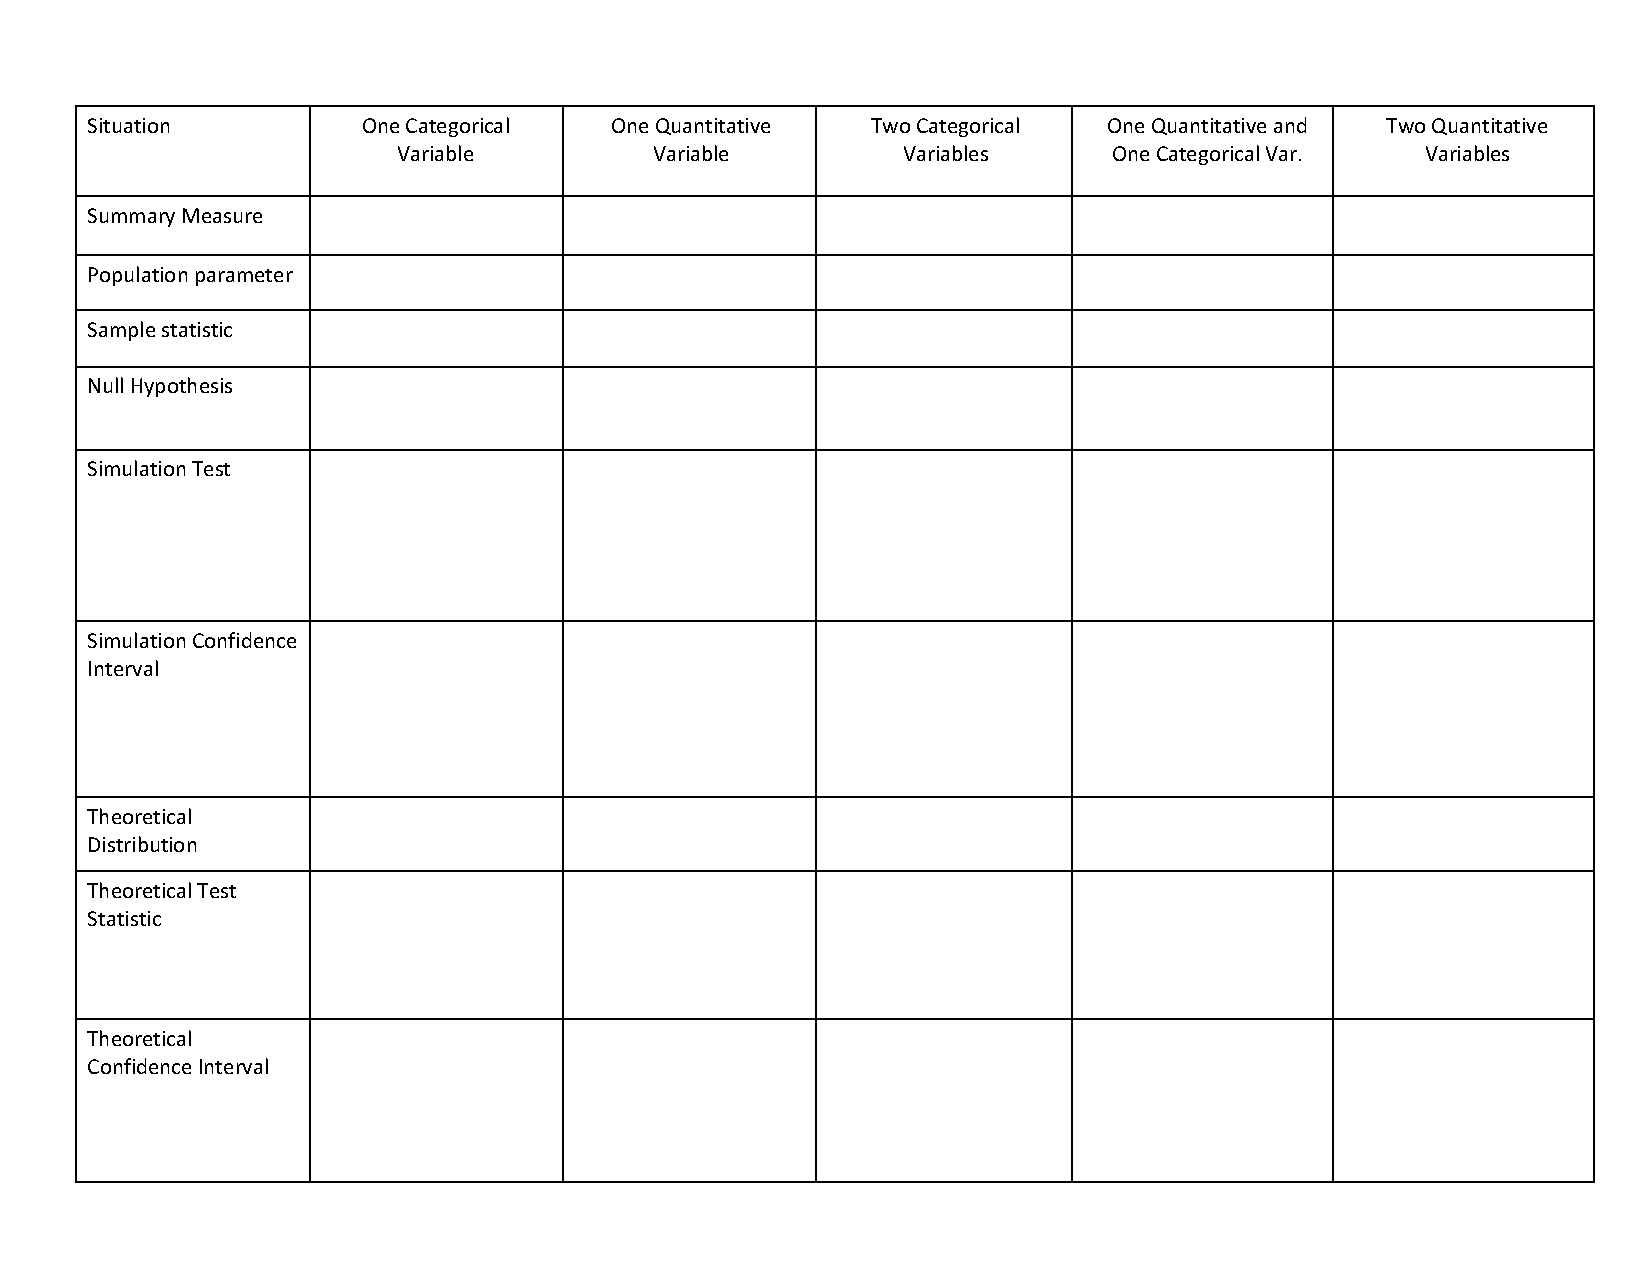
\includegraphics[angle = 90]{plots/ReviewTable.pdf}  %% p 253
    }
\end{figure}
\thispagestyle{empty}  %% Glossary  p  247 - 252
\fancyhead{}
%\newpage
%\ \ \ \thispagestyle{empty}
% \begin{figure}[p]
%     \vspace*{-1in}
%     \makebox[\linewidth]{
%         \includegraphics[angle = 90]{plots/ReviewTable.pdf}  %% p 253
%     }
% \end{figure}
\ \ \ \thispagestyle{empty}
\newpage
 \end{document}
